%&preformat-disser
\RequirePackage[l2tabu,orthodox]{nag} % Раскомментировав, можно в логе получать рекомендации относительно правильного использования пакетов и предупреждения об устаревших и нерекомендуемых пакетах
% Формат А4, 14pt (ГОСТ Р 7.0.11-2011, 5.3.6)
\documentclass[a4paper,14pt,oneside,openany]{memoir}

%%%%%%%%%%%%%%%%%%%%%%%%%%%%%%%%%%%%%%%%%%%%%%%%%%%%%%%%%%%%%%%%%%%%%%%%%%%%%%%%
%%%% Файл упрощённых настроек шаблона, общих для диссертации и автореферата %%%%
%%%%%%%%%%%%%%%%%%%%%%%%%%%%%%%%%%%%%%%%%%%%%%%%%%%%%%%%%%%%%%%%%%%%%%%%%%%%%%%%

%%% Режим черновика %%%
\makeatletter
\@ifundefined{c@draft}{
  \newcounter{draft}
  \setcounter{draft}{0}  % 0 --- чистовик (максимальное соблюдение ГОСТ)
                         % 1 --- черновик (отклонения от ГОСТ, но быстрая
                         %       сборка итоговых PDF)
}{}
\makeatother

%%% Пометки в тексте %%%
\makeatletter
\@ifundefined{c@showmarkup}{
  \newcounter{showmarkup}
  \setcounter{showmarkup}{0}  % 0 --- скрыть пометки
                              % 1 --- показывать пометки
}{}
\makeatother

%%% Использование в pdflatex шрифтов не по-умолчанию %%%
\makeatletter
\@ifundefined{c@usealtfont}{
  \newcounter{usealtfont}
  \setcounter{usealtfont}{1}    % 0 --- шрифты на базе Computer Modern
                                % 1 --- использовать пакет pscyr, при его
                                %       наличии
                                % 2 --- использовать пакет XCharter, при наличии
                                %       подходящей версии
}{}
\makeatother

%%% Использование в xelatex и lualatex семейств шрифтов %%%
\makeatletter
\@ifundefined{c@fontfamily}{
  \newcounter{fontfamily}
  \setcounter{fontfamily}{1}  % 0 --- CMU семейство. Используется как fallback;
                              % 1 --- Шрифты от MS (Times New Roman и компания)
                              % 2 --- Семейство Liberation
}{}
\makeatother

%%% Библиография %%%
\makeatletter
\@ifundefined{c@bibliosel}{
  \newcounter{bibliosel}
  \setcounter{bibliosel}{1}   % 0 --- встроенная реализация с загрузкой файла
                              %       через движок bibtex8;
                              % 1 --- реализация пакетом biblatex через движок
                              %       biber
}{}
\makeatother

%%% Вывод типов ссылок в библиографии %%%
\makeatletter
\@ifundefined{c@mediadisplay}{
  \newcounter{mediadisplay}
  \setcounter{mediadisplay}{2}   % 0 --- не делать ничего; надписи [Текст] и
                                 %       [Эл. ресурс] будут выводиться только в ссылках с
                                 %       заполненным полем `media`;
                                 % 1 --- автоматически добавлять надпись [Текст] к ссылкам с
                                 %       незаполненным полем `media`; таким образом, у всех
                                 %       источников будет указан тип, что соответствует
                                 %       требованиям ГОСТ
                                 % 2 --- автоматически удалять надписи [Текст], [Эл. Ресурс] и др.;
                                 %       не соответствует ГОСТ
                                 % 3 --- автоматически удалять надпись [Текст];
                                 %       не соответствует ГОСТ
                                 % 4 --- автоматически удалять надпись [Эл. Ресурс];
                                 %       не соответствует ГОСТ
}{}
\makeatother

%%% Предкомпиляция tikz рисунков для ускорения работы %%%
\makeatletter
\@ifundefined{c@imgprecompile}{
  \newcounter{imgprecompile}
  \setcounter{imgprecompile}{0}   % 0 --- без предкомпиляции;
                                  % 1 --- пользоваться предварительно
                                  %       скомпилированными pdf вместо генерации
                                  %       заново из tikz
}{}
\makeatother
            % общие настройки шаблона
%%% Проверка используемого TeX-движка %%%
\newif\ifxetexorluatex   % определяем новый условный оператор (http://tex.stackexchange.com/a/47579)
\ifxetex
    \xetexorluatextrue
\else
    \ifluatex
        \xetexorluatextrue
    \else
        \xetexorluatexfalse
    \fi
\fi

\newif\ifsynopsis           % Условие, проверяющее, что документ --- автореферат

\usepackage{etoolbox}[2015/08/02]   % Для продвинутой проверки разных условий
\providebool{presentation}

\usepackage{comment}    % Позволяет убирать блоки текста (добавляет
                        % окружение comment и команду \excludecomment)

%%% Поля и разметка страницы %%%
\usepackage{pdflscape}  % Для включения альбомных страниц
\usepackage{geometry}   % Для последующего задания полей

%%% Математические пакеты %%%
\usepackage{amsthm,amsmath,amscd}   % Математические дополнения от AMS
\usepackage{amsfonts,amssymb}       % Математические дополнения от AMS
\usepackage{mathtools}              % Добавляет окружение multlined
\usepackage{xfrac}                  % Красивые дроби
\usepackage[
    locale = DE,
    list-separator       = {;\,},
    list-final-separator = {;\,},
    list-pair-separator  = {;\,},
    list-units           = single,
    range-units          = single,
    range-phrase={\text{\ensuremath{-}}},
    % quotient-mode        = fraction, % красивые дроби могут не соответствовать ГОСТ
    fraction-function    = \sfrac,
    separate-uncertainty,
    ]{siunitx}[=v2]                 % Размерности SI
\sisetup{inter-unit-product = \ensuremath{{}\cdot{}}}

% Кириллица в нумерации subequations
% Для правильной работы требуется выполнение сразу после загрузки пакетов
\patchcmd{\subequations}{\def\theequation{\theparentequation\alph{equation}}}
{\def\theequation{\theparentequation\asbuk{equation}}}
{\typeout{subequations patched}}{\typeout{subequations not patched}}

%%%% Установки для размера шрифта 14 pt %%%%
%% Формирование переменных и констант для сравнения (один раз для всех подключаемых файлов)%%
%% должно располагаться до вызова пакета fontspec или polyglossia, потому что они сбивают его работу
\newlength{\curtextsize}
\newlength{\bigtextsize}
\setlength{\bigtextsize}{13.9pt}

\makeatletter
%\show\f@size    % неплохо для отслеживания, но вызывает стопорение процесса,
                 % если документ компилируется без команды  -interaction=nonstopmode
\setlength{\curtextsize}{\f@size pt}
\makeatother

%%% Кодировки и шрифты %%%
\ifxetexorluatex
    \ifpresentation
        \providecommand*\autodot{} % quick fix for polyglossia 1.50
    \fi
    \PassOptionsToPackage{no-math}{fontspec}    % https://tex.stackexchange.com/a/26295/104425
    \usepackage{polyglossia}[2014/05/21]        % Поддержка многоязычности
                                        % (fontspec подгружается автоматически)
\else
   %%% Решение проблемы копирования текста в буфер кракозябрами
    \ifnumequal{\value{usealtfont}}{0}{}{
        \input glyphtounicode.tex
        \input glyphtounicode-cmr.tex %from pdfx package
        \pdfgentounicode=1
    }
    \usepackage{cmap}   % Улучшенный поиск русских слов в полученном pdf-файле
    \ifnumequal{\value{usealtfont}}{2}{}{
        \defaulthyphenchar=127  % Если стоит до fontenc, то переносы
                                % не впишутся в выделяемый текст при
                                % копировании его в буфер обмена
    }
    \usepackage{textcomp}
    \usepackage[T1,T2A]{fontenc}                    % Поддержка русских букв
    \ifnumequal{\value{usealtfont}}{1}{% Используется pscyr, при наличии
        \IfFileExists{pscyr.sty}{\usepackage{pscyr}}{}  % Подключение pscyr
    }{}
    \usepackage[utf8]{inputenc}[2014/04/30]         % Кодировка utf8
    \usepackage[english, russian]{babel}[2014/03/24]% Языки: русский, английский
    \makeatletter\AtBeginDocument{\let\@elt\relax}\makeatother % babel 3.40 fix
    \ifnumequal{\value{usealtfont}}{2}{
        % http://dxdy.ru/post1238763.html#p1238763
        \usepackage[scaled=0.914]{XCharter}[2017/12/19] % Подключение русифицированных шрифтов XCharter
        \usepackage[charter, vvarbb, scaled=1.048]{newtxmath}[2017/12/14]
        \ifpresentation
        \else
            \setDisplayskipStretch{-0.078}
        \fi
    }{}
\fi

%%% Оформление абзацев %%%
\ifpresentation
\else
    \indentafterchapter     % Красная строка после заголовков типа chapter
    \usepackage{indentfirst}
\fi

%%% Цвета %%%
\ifpresentation
\else
    \usepackage[dvipsnames, table, hyperref]{xcolor} % Совместимо с tikz
\fi

%%% Таблицы %%%
\usepackage{longtable} % Длинные таблицы
\usepackage{multirow,makecell}   % Улучшенное форматирование таблиц
\usepackage{tabulary,tabularray} % Таблицы с автоматически подбирающейся
                                 % шириной столбцов
\UseTblrLibrary{booktabs}
\ExplSyntaxOn% define \IfTokenListEmpty to use \captionof with tabularray
\prg_generate_conditional_variant:Nnn \tl_if_empty:n { e } { TF }
\let \IfTokenListEmpty = \tl_if_empty:eTF
\ExplSyntaxOff

\usepackage{threeparttable}      % автоматический подгон ширины подписи таблицы

%%% Общее форматирование
%\usepackage{soul}% Поддержка переносоустойчивых подчёркиваний и зачёркиваний
\usepackage{icomma}  % Запятая в десятичных дробях

%%% Оптимизация расстановки переносов и длины последней строки абзаца
\IfFileExists{impnattypo.sty}{% проверка установленности пакета impnattypo
    \ifluatex
        \ifnumequal{\value{draft}}{1}{% Черновик
            \usepackage[hyphenation, lastparline, nosingleletter, homeoarchy,
            rivers, draft]{impnattypo}
        }{% Чистовик
            \usepackage[hyphenation, lastparline, nosingleletter]{impnattypo}
        }
    \else
        \usepackage[hyphenation, lastparline]{impnattypo}
    \fi
}{}

%% Векторная графика

\usepackage{tikz}                   % Продвинутый пакет векторной графики
\usetikzlibrary{chains}             % Для примера tikz рисунка
\usetikzlibrary{shapes.geometric}   % Для примера tikz рисунка
\usetikzlibrary{shapes.symbols}     % Для примера tikz рисунка
\usetikzlibrary{arrows}             % Для примера tikz рисунка

\usepackage[european,cuteinductors]{circuitikz} % Электрические схемы
\usepackage{pgfplots}                           % Графики
\pgfplotsset{compat=newest}
\usepgfplotslibrary{groupplots,units}
\pgfkeys{/pgf/number format/.cd,use comma,1000 sep={}} % форматирование чисел в графиках

%%% Гиперссылки %%%
\ifxetexorluatex
    \let\CYRDZE\relax
\fi
\usepackage{hyperref}[2012/11/06]

%%% Изображения %%%
\usepackage{graphicx}[2014/04/25]   % Подключаем пакет работы с графикой
\usepackage{caption}                % Подписи рисунков и таблиц
\usepackage{subcaption}             % Подписи подрисунков и подтаблиц
\usepackage{pdfpages}               % Добавление внешних pdf файлов

%%% Счётчики %%%
\usepackage{aliascnt}
\usepackage[figure,table]{totalcount}   % Счётчик рисунков и таблиц
\usepackage{totcount}   % Пакет создания счётчиков на основе последнего номера
                        % подсчитываемого элемента (может требовать дважды
                        % компилировать документ)
\usepackage{totpages}   % Счётчик страниц, совместимый с hyperref (ссылается
                        % на номер последней страницы). Желательно ставить
                        % последним пакетом в преамбуле

%%% Продвинутое управление групповыми ссылками (пока только формулами) %%%
\ifpresentation
\else
    \usepackage[russian]{cleveref} % cleveref имеет сложности со считыванием
    % языка из babel. Такое решение русификации вывода выбрано вместо
    % определения в documentclass из опасности что-то лишнее передать во все
    % остальные пакеты, включая библиографию.

    % Добавление возможности использования пробелов в \labelcref
    % https://tex.stackexchange.com/a/340502/104425
    \usepackage{kvsetkeys}
    \makeatletter
    \let\org@@cref\@cref
    \renewcommand*{\@cref}[2]{%
        \edef\process@me{%
            \noexpand\org@@cref{#1}{\zap@space#2 \@empty}%
        }\process@me
    }
    \makeatother
\fi

\usepackage{placeins} % для \FloatBarrier

\ifnumequal{\value{draft}}{1}{% Черновик
    \usepackage[firstpage]{draftwatermark}
    \SetWatermarkText{DRAFT}
    \SetWatermarkFontSize{14pt}
    \SetWatermarkScale{15}
    \SetWatermarkAngle{45}
}{}

%%% Цитата, не приводимая в автореферате:
% возможно, актуальна только для biblatex
%\newcommand{\citeinsynopsis}[1]{\ifsynopsis\else ~\cite{#1} \fi}

% если текущий процесс запущен библиотекой tikz-external, то прекомпиляция должна быть включена
\ifdefined\tikzexternalrealjob
    \setcounter{imgprecompile}{1}
\fi

\ifnumequal{\value{imgprecompile}}{1}{% Только если у нас включена предкомпиляция
    \usetikzlibrary{external}   % подключение возможности предкомпиляции
    \tikzexternalize[prefix=images/cache/,optimize command away=\includepdf] % activate! % здесь можно указать отдельную папку для скомпилированных файлов
    \ifxetex
        \tikzset{external/up to date check={diff}}
    \fi
}{}
         % Пакеты общие для диссертации и автореферата
\synopsisfalse                      % Этот документ --- не автореферат
\input{Dissertation/dispackages}    % Пакеты для диссертации
\usepackage{fr-longtable}    %ради \endlasthead

% Листинги с исходным кодом программ
\usepackage{fancyvrb}
\usepackage{listings}
\lccode`\~=0\relax %Без этого хака из-за особенностей пакета listings перестают работать конструкции с \MakeLowercase и т. п. в (xe|lua)latex

% Русская традиция начертания греческих букв
\usepackage{upgreek} % прямые греческие ради русской традиции

\usepackage{amssymb,amsmath,amsthm, amsfonts}

\newtheorem{thm}{Theorem}[section]
\newtheorem{proposition}[thm]{Утверждение}
\newtheorem{corollary}[thm]{Следствие}
\newtheorem{lemma}[thm]{Лемма}
\newtheorem{remark}[thm]{Замечание}
\newtheorem{example}[thm]{Пример}
\newtheorem{definition}[thm]{Определение}
\newtheorem{theorem}[thm]{Теорема}

%%% Микротипографика
%\ifnumequal{\value{draft}}{0}{% Только если у нас режим чистовика
%    \usepackage[final, babel, shrink=45]{microtype}[2016/05/14] % улучшает представление букв и слов в строках, может помочь при наличии отдельно висящих слов
%}{}

% Отметка о версии черновика на каждой странице
% Чтобы работало надо в своей локальной копии по инструкции
% https://www.ctan.org/pkg/gitinfo2 создать небходимые файлы в папке
% ./git/hooks
% If you’re familiar with tweaking git, you can probably work it out for
% yourself. If not, I suggest you follow these steps:
% 1. First, you need a git repository and working tree. For this example,
% let’s suppose that the root of the working tree is in ~/compsci
% 2. Copy the file post-xxx-sample.txt (which is in the same folder of
% your TEX distribution as this pdf) into the git hooks directory in your
% working copy. In our example case, you should end up with a file called
% ~/compsci/.git/hooks/post-checkout
% 3. If you’re using a unix-like system, don’t forget to make the file executable.
% Just how you do this is outside the scope of this manual, but one
% possible way is with commands such as this:
% chmod g+x post-checkout.
% 4. Test your setup with “git checkout master” (or another suitable branch
% name). This should generate copies of gitHeadInfo.gin in the directories
% you intended.
% 5. Now make two more copies of this file in the same directory (hooks),
% calling them post-commit and post-merge, and you’re done. As before,
% users of unix-like systems should ensure these files are marked as
% executable.
\ifnumequal{\value{draft}}{1}{% Черновик
   \IfFileExists{.git/gitHeadInfo.gin}{
      \usepackage[mark,pcount]{gitinfo2}
      \renewcommand{\gitMark}{rev.\gitAbbrevHash\quad\gitCommitterEmail\quad\gitAuthorIsoDate}
      \renewcommand{\gitMarkFormat}{\rmfamily\color{Gray}\small\bfseries}
   }{}
}{}   % Пакеты для специфических пользовательских задач

%%%%%%%%%%%%%%%%%%%%%%%%%%%%%%%%%%%%%%%%%%%%%%%%%%%%%%%
%%%% Файл упрощённых настроек шаблона автореферата %%%%
%%%%%%%%%%%%%%%%%%%%%%%%%%%%%%%%%%%%%%%%%%%%%%%%%%%%%%%

%%% Инициализирование переменных, не трогать!  %%%
\newcounter{showperssign}
\newcounter{showsecrsign}
\newcounter{showopplead}
%%%%%%%%%%%%%%%%%%%%%%%%%%%%%%%%%%%%%%%%%%%%%%%%%%%%%%%

%%% Список публикаций %%%
\makeatletter
\@ifundefined{c@usefootcite}{
  \newcounter{usefootcite}
  \setcounter{usefootcite}{0} % 0 --- два списка литературы;
                              % 1 --- список публикаций автора + цитирование
                              %       других работ в сносках
}{}
\makeatother

\makeatletter
\@ifundefined{c@bibgrouped}{
  \newcounter{bibgrouped}
  \setcounter{bibgrouped}{0}  % 0 --- единый список работ автора;
                              % 1 --- сгруппированные работы автора
}{}
\makeatother

%%% Область упрощённого управления оформлением %%%

%% Управление зазором между подрисуночной подписью и основным текстом %%
\setlength{\belowcaptionskip}{10pt plus 20pt minus 2pt}


%% Подпись таблиц %%

% смещение строк подписи после первой
\newcommand{\tabindent}{0cm}

% тип форматирования таблицы
% plain --- название и текст в одной строке
% split --- название и текст в разных строках
\newcommand{\tabformat}{plain}

%%% настройки форматирования таблицы `plain'

% выравнивание по центру подписи, состоящей из одной строки
% true  --- выравнивать
% false --- не выравнивать
\newcommand{\tabsinglecenter}{false}

% выравнивание подписи таблиц
% justified   --- выравнивать как обычный текст
% centering   --- выравнивать по центру
% centerlast  --- выравнивать по центру только последнюю строку
% centerfirst --- выравнивать по центру только первую строку
% raggedleft  --- выравнивать по правому краю
% raggedright --- выравнивать по левому краю
\newcommand{\tabjust}{justified}

% Разделитель записи «Таблица #» и названия таблицы
\newcommand{\tablabelsep}{~\cyrdash\ }

%%% настройки форматирования таблицы `split'

% положение названия таблицы
% \centering   --- выравнивать по центру
% \raggedleft  --- выравнивать по правому краю
% \raggedright --- выравнивать по левому краю
\newcommand{\splitformatlabel}{\raggedleft}

% положение текста подписи
% \centering   --- выравнивать по центру
% \raggedleft  --- выравнивать по правому краю
% \raggedright --- выравнивать по левому краю
\newcommand{\splitformattext}{\raggedright}

%% Подпись рисунков %%
%Разделитель записи «Рисунок #» и названия рисунка
\newcommand{\figlabelsep}{~\cyrdash\ }  % (ГОСТ 2.105, 4.3.1)
                                        % "--- здесь не работает

%Демонстрация подписи диссертанта на автореферате
\setcounter{showperssign}{1}  % 0 --- не показывать;
                              % 1 --- показывать
%Демонстрация подписи учёного секретаря на автореферате
\setcounter{showsecrsign}{0}  % 0 --- не показывать;
                              % 1 --- показывать
%Демонстрация информации об оппонентах и ведущей организации на автореферате
\setcounter{showopplead}{1}   % 0 --- не показывать;
                              % 1 --- показывать

%%% Цвета гиперссылок %%%
% Latex color definitions: http://latexcolor.com/
\definecolor{linkcolor}{rgb}{0.9,0,0}
\definecolor{citecolor}{rgb}{0,0.6,0}
\definecolor{urlcolor}{rgb}{0,0,1}
%\definecolor{linkcolor}{rgb}{0,0,0} %black
%\definecolor{citecolor}{rgb}{0,0,0} %black
%\definecolor{urlcolor}{rgb}{0,0,0} %black
      % Упрощённые настройки шаблона

% Новые переменные, которые могут использоваться во всём проекте
% ГОСТ 7.0.11-2011
% 9.2 Оформление текста автореферата диссертации
% 9.2.1 Общая характеристика работы включает в себя следующие основные структурные
% элементы:
% актуальность темы исследования;
\newcommand{\actualityTXT}{Актуальность и степень разработанности темы.}
% степень ее разработанности;
\newcommand{\progressTXT}{Степень разработанности темы.}
% цели и задачи;
\newcommand{\aimTXT}{Целью}
\newcommand{\tasksTXT}{задачи}
% научную новизну;
\newcommand{\noveltyTXT}{Научная новизна:}
% теоретическую и практическую значимость работы;
\newcommand{\influenceTXT}{Теоретическая и практическая значимость.}
% или чаще используют просто
%\newcommand{\influenceTXT}{Практическая значимость}
% методологию и методы исследования;
\newcommand{\methodsTXT}{Методология и методы исследования.}
% положения, выносимые на защиту;
\newcommand{\defpositionsTXT}{Основные положения, выносимые на~защиту:}
% степень достоверности и апробацию результатов.
\newcommand{\reliabilityTXT}{Достоверность}
\newcommand{\probationTXT}{Апробация работы.}

\newcommand{\contributionTXT}{Личный вклад.}
\newcommand{\publicationsTXT}{Публикации.}


% актуальность темы исследования;
\newcommand{\actualityTXTEng}{PhD Dissertation Relevance.}
% степень ее разработанности;
%\newcommand{\progressTXTEng}{Степень разработанности темы.}
% цели и задачи;
\newcommand{\aimTXTEng}{aim}
\newcommand{\tasksTXTEng}{tasks}
% научную новизну;
\newcommand{\noveltyTXTEng}{Novelty:}
% теоретическую и практическую значимость работы;
\newcommand{\influenceTXTEng}{Theoretical and Practical Value.}
% или чаще используют просто
%\newcommand{\influenceTXT}{Практическая значимость}
% методологию и методы исследования;
\newcommand{\methodsTXTEng}{Methodology and Research Methods.}
% положения, выносимые на защиту;
\newcommand{\defpositionsTXTEng}{Key aspects that are submitted for defence:}
% степень достоверности и апробацию результатов.
\newcommand{\reliabilityTXTEng}{reliability}
\newcommand{\probationTXTEng}{Aprobation of the work.}

\newcommand{\contributionTXTEng}{Personal Contribution.}
\newcommand{\publicationsTXTEng}{Publications.}


%%% Заголовки библиографии:

% для автореферата:
\newcommand{\bibtitleauthor}{Публикации автора по теме диссертации}
\newcommand{\bibtitleauthorEng}{Publications}

% для стиля библиографии `\insertbiblioauthorgrouped`
\newcommand{\bibtitleauthorvak}{В изданиях из списка ВАК РФ}
\newcommand{\bibtitleauthorscopus}{В изданиях, входящих в международную базу цитирования Scopus}
\newcommand{\bibtitleauthorwos}{В изданиях, входящих в международную базу цитирования Web of Science}
\newcommand{\bibtitleauthorother}{В прочих изданиях}
\newcommand{\bibtitleauthorconf}{В сборниках трудов конференций}
\newcommand{\bibtitleauthorpatent}{Зарегистрированные патенты}
\newcommand{\bibtitleauthorprogram}{Зарегистрированные программы для ЭВМ}

% для стиля библиографии `\insertbiblioauthorimportant`:
\newcommand{\bibtitleauthorimportant}{Наиболее значимые \protect\MakeLowercase\bibtitleauthor}

% для списка литературы в диссертации и списка чужих работ в автореферате:
\newcommand{\bibtitlefull}{Список литературы} % (ГОСТ Р 7.0.11-2011, 4)
\newcommand{\bibtitlefullEng}{Bibliography} % (ГОСТ Р 7.0.11-2011, 4)
         % Новые переменные, для всего проекта

%%% Основные сведения %%%
\newcommand{\thesisAuthorLastName}{Алексеев}
\newcommand{\thesisAuthorOtherNames}{Владислав Владимирович}
\newcommand{\thesisAuthorInitials}{В.\,В.}
\newcommand{\thesisAuthor}             % Диссертация, ФИО автора
{%
    \texorpdfstring{% \texorpdfstring takes two arguments and uses the first for (La)TeX and the second for pdf
        \thesisAuthorLastName~\thesisAuthorOtherNames% так будет отображаться на титульном листе или в тексте, где будет использоваться переменная
    }{%
        \thesisAuthorLastName, \thesisAuthorOtherNames% эта запись для свойств pdf-файла. В таком виде, если pdf будет обработан программами для сбора библиографических сведений, будет правильно представлена фамилия.
    }
}
\newcommand{\thesisAuthorShort}        % Диссертация, ФИО автора инициалами
{\thesisAuthorInitials~\thesisAuthorLastName}
%\newcommand{\thesisUdk}                % Диссертация, УДК
%{\fixme{xxx.xxx}}
\newcommand{\thesisTitle}              % Диссертация, название
{Анализ сходимости периодического решения уравнения Мэки--Гласса к решению предельного уравнения}
\newcommand{\thesisSpecialtyNumber}    % Диссертация, специальность, номер
{01.01.02}
\newcommand{\thesisSpecialtyTitle}     % Диссертация, специальность, название (название взято с сайта ВАК для примера)
{Дифференциальные уравнения, динамические системы и оптимальное управление}
%% \newcommand{\thesisSpecialtyTwoNumber} % Диссертация, вторая специальность, номер
%% {\fixme{XX.XX.XX}}
%% \newcommand{\thesisSpecialtyTwoTitle}  % Диссертация, вторая специальность, название
%% {\fixme{Теория и~методика физического воспитания, спортивной тренировки,
%% оздоровительной и~адаптивной физической культуры}}
\newcommand{\thesisDegree}             % Диссертация, ученая степень
{кандидата физико-математических наук}
\newcommand{\thesisDegreeShort}        % Диссертация, ученая степень, краткая запись
{канд. физ.-мат. наук}
\newcommand{\thesisCity}               % Диссертация, город написания диссертации
{Семинар по КТДУ, \newline МГУ, Москва}
\newcommand{\thesisYear}               % Диссертация, год написания диссертации
{29 ноября 2024 г.}
\newcommand{\thesisOrganization}       % Диссертация, организация
{Федеральное государственное бюджетное образовательное учреждение высшего образования <<Ярославский государственный университет им. П.Г. Демидова>>}
\newcommand{\thesisOrganizationShort}  % Диссертация, краткое название организации для доклада
{Периодические решения уравнения Мэки--Гласса}

\newcommand{\thesisInOrganization}     % Диссертация, организация в предложном падеже: Работа выполнена в ...
{Федеральном государственном бюджетном образовательном учреждении высшего образования <<Ярославский государственный университет им. П.Г. Демидова>>}

%% \newcommand{\supervisorDead}{}           % Рисовать рамку вокруг фамилии
\newcommand{\supervisorFio}              % Научный руководитель, ФИО
{Глызин Сергей Дмитриевич}
\newcommand{\supervisorRegalia}          % Научный руководитель, регалии
{доктор физ.-мат. наук, профессор}
\newcommand{\supervisorFioShort}         % Научный руководитель, ФИО
{С.\,Д.~Глызин}
\newcommand{\supervisorRegaliaShort}     % Научный руководитель, регалии
{д.~ф.-м.~н.,~проф.}

%% \newcommand{\supervisorTwoDead}{}        % Рисовать рамку вокруг фамилии
\newcommand{\supervisorTwoFio}           % Второй научный руководитель, ФИО
{Преображенская Маргарита Михайловна}
\newcommand{\supervisorTwoRegalia}       % Второй научный руководитель, регалии
{кандидат физ.-мат. наук}
\newcommand{\supervisorTwoFioShort}      % Второй научный руководитель, ФИО
{М.\,М.~Преображенская}
\newcommand{\supervisorTwoRegaliaShort}  % Второй научный руководитель, регалии
{к.~ф.-м.~н.}

\newcommand{\opponentOneFio}           % Оппонент 1, ФИО
{\fixme{Фамилия Имя Отчество}}
\newcommand{\opponentOneRegalia}       % Оппонент 1, регалии
{\fixme{доктор физико-математических наук, профессор}}
\newcommand{\opponentOneJobPlace}      % Оппонент 1, место работы
{\fixme{Не очень длинное название для места работы}}
\newcommand{\opponentOneJobPost}       % Оппонент 1, должность
{\fixme{старший научный сотрудник}}

\newcommand{\opponentTwoFio}           % Оппонент 2, ФИО
{\fixme{Фамилия Имя Отчество}}
\newcommand{\opponentTwoRegalia}       % Оппонент 2, регалии
{\fixme{кандидат физико-математических наук}}
\newcommand{\opponentTwoJobPlace}      % Оппонент 2, место работы
{\fixme{Основное место работы c длинным длинным длинным длинным названием}}
\newcommand{\opponentTwoJobPost}       % Оппонент 2, должность
{\fixme{старший научный сотрудник}}

%% \newcommand{\opponentThreeFio}         % Оппонент 3, ФИО
%% {\fixme{Фамилия Имя Отчество}}
%% \newcommand{\opponentThreeRegalia}     % Оппонент 3, регалии
%% {\fixme{кандидат физико-математических наук}}
%% \newcommand{\opponentThreeJobPlace}    % Оппонент 3, место работы
%% {\fixme{Основное место работы c длинным длинным длинным длинным названием}}
%% \newcommand{\opponentThreeJobPost}     % Оппонент 3, должность
%% {\fixme{старший научный сотрудник}}

\newcommand{\leadingOrganizationTitle} % Ведущая организация, дополнительные строки. Удалить, чтобы не отображать в автореферате
{\fixme{Федеральное государственное бюджетное образовательное учреждение высшего
профессионального образования с~длинным длинным длинным длинным названием}}

\newcommand{\defenseDate}              % Защита, дата
{\fixme{DD mmmmmmmm YYYY~г.~в~XX часов}}
\newcommand{\defenseCouncilNumber}     % Защита, номер диссертационного совета
{\fixme{Д\,123.456.78}}
\newcommand{\defenseCouncilTitle}      % Защита, учреждение диссертационного совета
{\fixme{Название учреждения}}
\newcommand{\defenseCouncilAddress}    % Защита, адрес учреждение диссертационного совета
{\fixme{Адрес}}
\newcommand{\defenseCouncilPhone}      % Телефон для справок
{\fixme{+7~(0000)~00-00-00}}

\newcommand{\defenseSecretaryFio}      % Секретарь диссертационного совета, ФИО
{\fixme{Фамилия Имя Отчество}}
\newcommand{\defenseSecretaryRegalia}  % Секретарь диссертационного совета, регалии
{\fixme{д-р~физ.-мат. наук}}            % Для сокращений есть ГОСТы, например: ГОСТ Р 7.0.12-2011 + http://base.garant.ru/179724/#block_30000

\newcommand{\synopsisLibrary}          % Автореферат, название библиотеки
{\fixme{Название библиотеки}}
\newcommand{\synopsisDate}             % Автореферат, дата рассылки
{\fixme{DD mmmmmmmm}\the\year~года}

% To avoid conflict with beamer class use \providecommand
\providecommand{\keywords}%            % Ключевые слова для метаданных PDF диссертации и автореферата
{}
             % Основные сведения
\input{common/fonts}            % Определение шрифтов (частичное)
%%% Шаблон %%%
\DeclareRobustCommand{\fixme}{\textcolor{red}}  % решаем проблему превращения
                                % названия цвета в результате \MakeUppercase,
                                % http://tex.stackexchange.com/a/187930,
                                % \DeclareRobustCommand protects \fixme
                                % from expanding inside \MakeUppercase
\AtBeginDocument{%
    \setlength{\parindent}{2.5em}                   % Абзацный отступ. Должен быть одинаковым по всему тексту и равен пяти знакам (ГОСТ Р 7.0.11-2011, 5.3.7).
}

%%% Таблицы %%%
\DeclareCaptionLabelSeparator{tabsep}{\tablabelsep} % нумерация таблиц
\DeclareCaptionFormat{split}{\splitformatlabel#1\par\splitformattext#3}

\captionsetup[table]{
        format=\tabformat,                % формат подписи (plain|hang)
        font=normal,                      % нормальные размер, цвет, стиль шрифта
        skip=.0pt,                        % отбивка под подписью
        parskip=.0pt,                     % отбивка между параграфами подписи
        position=above,                   % положение подписи
        justification=\tabjust,           % центровка
        indent=\tabindent,                % смещение строк после первой
        labelsep=tabsep,                  % разделитель
        singlelinecheck=\tabsinglecenter, % не выравнивать по центру, если умещается в одну строку
}

%%% Рисунки %%%
\DeclareCaptionLabelSeparator{figsep}{\figlabelsep} % нумерация рисунков

\captionsetup[figure]{
        format=plain,                     % формат подписи (plain|hang)
        font=normal,                      % нормальные размер, цвет, стиль шрифта
        skip=.0pt,                        % отбивка под подписью
        parskip=.0pt,                     % отбивка между параграфами подписи
        position=below,                   % положение подписи
        singlelinecheck=true,             % выравнивание по центру, если умещается в одну строку
        justification=centerlast,         % центровка
        labelsep=figsep,                  % разделитель
		width=0.9\textwidth				  % ширина подписи
}

%%% Подписи подрисунков %%%
\DeclareCaptionSubType{figure}
\renewcommand\thesubfigure{\asbuk{subfigure}} % нумерация подрисунков
\ifsynopsis
\DeclareCaptionFont{norm}{\fontsize{10pt}{11pt}\selectfont}
\newcommand{\subfigureskip}{2.pt}
\else
\DeclareCaptionFont{norm}{\fontsize{14pt}{16pt}\selectfont}
\newcommand{\subfigureskip}{0.pt}
\fi

\captionsetup[subfloat]{
        labelfont=norm,                 % нормальный размер подписей подрисунков
        textfont=norm,                  % нормальный размер подписей подрисунков
        labelsep=space,                 % разделитель
        labelformat=brace,              % одна скобка справа от номера
        justification=centering,        % центровка
        singlelinecheck=true,           % выравнивание по центру, если умещается в одну строку
        skip=\subfigureskip,            % отбивка над подписью
        parskip=.0pt,                   % отбивка между параграфами подписи
        position=below,                 % положение подписи
}

%%% Настройки ссылок на рисунки, таблицы и др. %%%
% команды \cref...format отвечают за форматирование при помощи команды \cref
% команды \labelcref...format отвечают за форматирование при помощи команды \labelcref

\ifpresentation
\else
    \crefdefaultlabelformat{#2#1#3}

    % Уравнение
    \crefformat{equation}{(#2#1#3)} % одиночная ссылка с приставкой
    \labelcrefformat{equation}{(#2#1#3)} % одиночная ссылка без приставки
    \crefrangeformat{equation}{(#3#1#4) \cyrdash~(#5#2#6)} % диапазон ссылок с приставкой
    \labelcrefrangeformat{equation}{(#3#1#4) \cyrdash~(#5#2#6)} % диапазон ссылок без приставки
    \crefmultiformat{equation}{(#2#1#3)}{ и~(#2#1#3)}{, (#2#1#3)}{ и~(#2#1#3)} % перечисление ссылок с приставкой
    \labelcrefmultiformat{equation}{(#2#1#3)}{ и~(#2#1#3)}{, (#2#1#3)}{ и~(#2#1#3)} % перечисление без приставки

    % Подуравнение
    \crefformat{subequation}{(#2#1#3)} % одиночная ссылка с приставкой
    \labelcrefformat{subequation}{(#2#1#3)} % одиночная ссылка без приставки
    \crefrangeformat{subequation}{(#3#1#4) \cyrdash~(#5#2#6)} % диапазон ссылок с приставкой
    \labelcrefrangeformat{subequation}{(#3#1#4) \cyrdash~(#5#2#6)} % диапазон ссылок без приставки
    \crefmultiformat{subequation}{(#2#1#3)}{ и~(#2#1#3)}{, (#2#1#3)}{ и~(#2#1#3)} % перечисление ссылок с приставкой
    \labelcrefmultiformat{subequation}{(#2#1#3)}{ и~(#2#1#3)}{, (#2#1#3)}{ и~(#2#1#3)} % перечисление без приставки

    % Глава
    \crefformat{chapter}{#2#1#3} % одиночная ссылка с приставкой
    \labelcrefformat{chapter}{#2#1#3} % одиночная ссылка без приставки
    \crefrangeformat{chapter}{#3#1#4 \cyrdash~#5#2#6} % диапазон ссылок с приставкой
    \labelcrefrangeformat{chapter}{#3#1#4 \cyrdash~#5#2#6} % диапазон ссылок без приставки
    \crefmultiformat{chapter}{#2#1#3}{ и~#2#1#3}{, #2#1#3}{ и~#2#1#3} % перечисление ссылок с приставкой
    \labelcrefmultiformat{chapter}{#2#1#3}{ и~#2#1#3}{, #2#1#3}{ и~#2#1#3} % перечисление без приставки

    % Параграф
    \crefformat{section}{#2#1#3} % одиночная ссылка с приставкой
    \labelcrefformat{section}{#2#1#3} % одиночная ссылка без приставки
    \crefrangeformat{section}{#3#1#4 \cyrdash~#5#2#6} % диапазон ссылок с приставкой
    \labelcrefrangeformat{section}{#3#1#4 \cyrdash~#5#2#6} % диапазон ссылок без приставки
    \crefmultiformat{section}{#2#1#3}{ и~#2#1#3}{, #2#1#3}{ и~#2#1#3} % перечисление ссылок с приставкой
    \labelcrefmultiformat{section}{#2#1#3}{ и~#2#1#3}{, #2#1#3}{ и~#2#1#3} % перечисление без приставки

    % Приложение
    \crefformat{appendix}{#2#1#3} % одиночная ссылка с приставкой
    \labelcrefformat{appendix}{#2#1#3} % одиночная ссылка без приставки
    \crefrangeformat{appendix}{#3#1#4 \cyrdash~#5#2#6} % диапазон ссылок с приставкой
    \labelcrefrangeformat{appendix}{#3#1#4 \cyrdash~#5#2#6} % диапазон ссылок без приставки
    \crefmultiformat{appendix}{#2#1#3}{ и~#2#1#3}{, #2#1#3}{ и~#2#1#3} % перечисление ссылок с приставкой
    \labelcrefmultiformat{appendix}{#2#1#3}{ и~#2#1#3}{, #2#1#3}{ и~#2#1#3} % перечисление без приставки

    % Рисунок
    \crefformat{figure}{#2#1#3} % одиночная ссылка с приставкой
    \labelcrefformat{figure}{#2#1#3} % одиночная ссылка без приставки
    \crefrangeformat{figure}{#3#1#4 \cyrdash~#5#2#6} % диапазон ссылок с приставкой
    \labelcrefrangeformat{figure}{#3#1#4 \cyrdash~#5#2#6} % диапазон ссылок без приставки
    \crefmultiformat{figure}{#2#1#3}{ и~#2#1#3}{, #2#1#3}{ и~#2#1#3} % перечисление ссылок с приставкой
    \labelcrefmultiformat{figure}{#2#1#3}{ и~#2#1#3}{, #2#1#3}{ и~#2#1#3} % перечисление без приставки

    % Таблица
    \crefformat{table}{#2#1#3} % одиночная ссылка с приставкой
    \labelcrefformat{table}{#2#1#3} % одиночная ссылка без приставки
    \crefrangeformat{table}{#3#1#4 \cyrdash~#5#2#6} % диапазон ссылок с приставкой
    \labelcrefrangeformat{table}{#3#1#4 \cyrdash~#5#2#6} % диапазон ссылок без приставки
    \crefmultiformat{table}{#2#1#3}{ и~#2#1#3}{, #2#1#3}{ и~#2#1#3} % перечисление ссылок с приставкой
    \labelcrefmultiformat{table}{#2#1#3}{ и~#2#1#3}{, #2#1#3}{ и~#2#1#3} % перечисление без приставки

    % Листинг
    \crefformat{lstlisting}{#2#1#3} % одиночная ссылка с приставкой
    \labelcrefformat{lstlisting}{#2#1#3} % одиночная ссылка без приставки
    \crefrangeformat{lstlisting}{#3#1#4 \cyrdash~#5#2#6} % диапазон ссылок с приставкой
    \labelcrefrangeformat{lstlisting}{#3#1#4 \cyrdash~#5#2#6} % диапазон ссылок без приставки
    \crefmultiformat{lstlisting}{#2#1#3}{ и~#2#1#3}{, #2#1#3}{ и~#2#1#3} % перечисление ссылок с приставкой
    \labelcrefmultiformat{lstlisting}{#2#1#3}{ и~#2#1#3}{, #2#1#3}{ и~#2#1#3} % перечисление без приставки

    % Листинг
    \crefformat{ListingEnv}{#2#1#3} % одиночная ссылка с приставкой
    \labelcrefformat{ListingEnv}{#2#1#3} % одиночная ссылка без приставки
    \crefrangeformat{ListingEnv}{#3#1#4 \cyrdash~#5#2#6} % диапазон ссылок с приставкой
    \labelcrefrangeformat{ListingEnv}{#3#1#4 \cyrdash~#5#2#6} % диапазон ссылок без приставки
    \crefmultiformat{ListingEnv}{#2#1#3}{ и~#2#1#3}{, #2#1#3}{ и~#2#1#3} % перечисление ссылок с приставкой
    \labelcrefmultiformat{ListingEnv}{#2#1#3}{ и~#2#1#3}{, #2#1#3}{ и~#2#1#3} % перечисление без приставки
\fi

%%% Настройки гиперссылок %%%
\ifluatex
    \hypersetup{
        unicode,                % Unicode encoded PDF strings
    }
\fi

\hypersetup{
    linktocpage=true,           % ссылки с номера страницы в оглавлении, списке таблиц и списке рисунков
    plainpages=false,           % Forces page anchors to be named by the Arabic form  of the page number, rather than the formatted form
    colorlinks,                 % ссылки отображаются раскрашенным текстом, а не раскрашенным прямоугольником, вокруг текста
    linkcolor={linkcolor},      % цвет ссылок типа ref, eqref и подобных
    citecolor={citecolor},      % цвет ссылок-цитат
    urlcolor={urlcolor},        % цвет гиперссылок
    pdftitle={\thesisTitle},    % Заголовок
    pdfauthor={\thesisAuthor},  % Автор
    pdfsubject={\thesisSpecialtyNumber\ \thesisSpecialtyTitle},      % Тема
    pdfkeywords={\keywords},    % Ключевые слова
    pdflang={ru},
}
\ifnumequal{\value{draft}}{1}{% Черновик
    \hypersetup{
        draft,
    }
}{}

%%% Списки %%%
% Используем короткое тире (endash) для ненумерованных списков (ГОСТ 2.105-95, пункт 4.1.7, требует дефиса, но так лучше смотрится)
\renewcommand{\labelitemi}{\normalfont\bfseries{--}}

% Перечисление строчными буквами латинского алфавита (ГОСТ 2.105-95, 4.1.7)
%\renewcommand{\theenumi}{\alph{enumi}}
%\renewcommand{\labelenumi}{\theenumi)}

% Перечисление строчными буквами русского алфавита (ГОСТ 2.105-95, 4.1.7)
\makeatletter
\AddEnumerateCounter{\asbuk}{\russian@alph}{щ}      % Управляем списками/перечислениями через пакет enumitem, а он 'не знает' про asbuk, потому 'учим' его
\makeatother
%\renewcommand{\theenumi}{\asbuk{enumi}} %первый уровень нумерации
%\renewcommand{\labelenumi}{\theenumi)} %первый уровень нумерации
\renewcommand{\theenumii}{\asbuk{enumii}} %второй уровень нумерации
\renewcommand{\labelenumii}{\theenumii)} %второй уровень нумерации
\renewcommand{\theenumiii}{\arabic{enumiii}} %третий уровень нумерации
\renewcommand{\labelenumiii}{\theenumiii)} %третий уровень нумерации

\setlist{nosep,%                                    % Единый стиль для всех списков (пакет enumitem), без дополнительных интервалов.
    labelindent=\parindent,leftmargin=*%            % Каждый пункт, подпункт и перечисление записывают с абзацного отступа (ГОСТ 2.105-95, 4.1.8)
}

%%% Правильная нумерация приложений, рисунков и формул %%%
%% По ГОСТ 2.105, п. 4.3.8 Приложения обозначают заглавными буквами русского алфавита,
%% начиная с А, за исключением букв Ё, З, Й, О, Ч, Ь, Ы, Ъ.
%% Здесь также переделаны все нумерации русскими буквами.
\ifxetexorluatex
    \makeatletter
    \def\russian@Alph#1{\ifcase#1\or
       А\or Б\or В\or Г\or Д\or Е\or Ж\or
       И\or К\or Л\or М\or Н\or
       П\or Р\or С\or Т\or У\or Ф\or Х\or
       Ц\or Ш\or Щ\or Э\or Ю\or Я\else\xpg@ill@value{#1}{russian@Alph}\fi}
    \def\russian@alph#1{\ifcase#1\or
       а\or б\or в\or г\or д\or е\or ж\or
       и\or к\or л\or м\or н\or
       п\or р\or с\or т\or у\or ф\or х\or
       ц\or ш\or щ\or э\or ю\or я\else\xpg@ill@value{#1}{russian@alph}\fi}
    \def\cyr@Alph#1{\ifcase#1\or
        А\or Б\or В\or Г\or Д\or Е\or Ж\or
        И\or К\or Л\or М\or Н\or
        П\or Р\or С\or Т\or У\or Ф\or Х\or
        Ц\or Ш\or Щ\or Э\or Ю\or Я\else\xpg@ill@value{#1}{cyr@Alph}\fi}
    \def\cyr@alph#1{\ifcase#1\or
        а\or б\or в\or г\or д\or е\or ж\or
        и\or к\or л\or м\or н\or
        п\or р\or с\or т\or у\or ф\or х\or
        ц\or ш\or щ\or э\or ю\or я\else\xpg@ill@value{#1}{cyr@alph}\fi}
    \makeatother
\else
    \makeatletter
    \if@uni@ode
      \def\russian@Alph#1{\ifcase#1\or
        А\or Б\or В\or Г\or Д\or Е\or Ж\or
        И\or К\or Л\or М\or Н\or
        П\or Р\or С\or Т\or У\or Ф\or Х\or
        Ц\or Ш\or Щ\or Э\or Ю\or Я\else\@ctrerr\fi}
    \else
      \def\russian@Alph#1{\ifcase#1\or
        \CYRA\or\CYRB\or\CYRV\or\CYRG\or\CYRD\or\CYRE\or\CYRZH\or
        \CYRI\or\CYRK\or\CYRL\or\CYRM\or\CYRN\or
        \CYRP\or\CYRR\or\CYRS\or\CYRT\or\CYRU\or\CYRF\or\CYRH\or
        \CYRC\or\CYRSH\or\CYRSHCH\or\CYREREV\or\CYRYU\or
        \CYRYA\else\@ctrerr\fi}
    \fi
    \if@uni@ode
      \def\russian@alph#1{\ifcase#1\or
        а\or б\or в\or г\or д\or е\or ж\or
        и\or к\or л\or м\or н\or
        п\or р\or с\or т\or у\or ф\or х\or
        ц\or ш\or щ\or э\or ю\or я\else\@ctrerr\fi}
    \else
      \def\russian@alph#1{\ifcase#1\or
        \cyra\or\cyrb\or\cyrv\or\cyrg\or\cyrd\or\cyre\or\cyrzh\or
        \cyri\or\cyrk\or\cyrl\or\cyrm\or\cyrn\or
        \cyrp\or\cyrr\or\cyrs\or\cyrt\or\cyru\or\cyrf\or\cyrh\or
        \cyrc\or\cyrsh\or\cyrshch\or\cyrerev\or\cyryu\or
        \cyrya\else\@ctrerr\fi}
    \fi
    \makeatother
\fi


%%http://www.linux.org.ru/forum/general/6993203#comment-6994589 (используется totcount)
\makeatletter
\def\formtotal#1#2#3#4#5{%
    \newcount\@c
    \@c\totvalue{#1}\relax
    \newcount\@last
    \newcount\@pnul
    \@last\@c\relax
    \divide\@last 10
    \@pnul\@last\relax
    \divide\@pnul 10
    \multiply\@pnul-10
    \advance\@pnul\@last
    \multiply\@last-10
    \advance\@last\@c
    #2%
    \ifnum\@pnul=1#5\else%
    \ifcase\@last#5\or#3\or#4\or#4\or#4\else#5\fi
    \fi
}
\makeatother

\newcommand{\formbytotal}[5]{\total{#1}~\formtotal{#1}{#2}{#3}{#4}{#5}}

%%% Команды рецензирования %%%
\ifboolexpr{ (test {\ifnumequal{\value{draft}}{1}}) or (test {\ifnumequal{\value{showmarkup}}{1}})}{
        \newrobustcmd{\todo}[1]{\textcolor{red}{#1}}
        \newrobustcmd{\note}[2][]{\ifstrempty{#1}{#2}{\textcolor{#1}{#2}}}
        \newenvironment{commentbox}[1][]%
        {\ifstrempty{#1}{}{\color{#1}}}%
        {}
}{
        \newrobustcmd{\todo}[1]{}
        \newrobustcmd{\note}[2][]{}
        \excludecomment{commentbox}
}
           % Стили общие для диссертации и автореферата
\input{Dissertation/disstyles}  % Стили для диссертации
% для вертикального центрирования ячеек в tabulary
\def\zz{\ifx\[$\else\aftergroup\zzz\fi}
%$ \] % <-- чиним подсветку синтаксиса в некоторых редакторах
\def\zzz{\setbox0\lastbox
\dimen0\dimexpr\extrarowheight + \ht0-\dp0\relax
\setbox0\hbox{\raise-.5\dimen0\box0}%
\ht0=\dimexpr\ht0+\extrarowheight\relax
\dp0=\dimexpr\dp0+\extrarowheight\relax
\box0
}

\lstdefinelanguage{Renhanced}%
{keywords={abbreviate,abline,abs,acos,acosh,action,add1,add,%
        aggregate,alias,Alias,alist,all,anova,any,aov,aperm,append,apply,%
        approx,approxfun,apropos,Arg,args,array,arrows,as,asin,asinh,%
        atan,atan2,atanh,attach,attr,attributes,autoload,autoloader,ave,%
        axis,backsolve,barplot,basename,besselI,besselJ,besselK,besselY,%
        beta,binomial,body,box,boxplot,break,browser,bug,builtins,bxp,by,%
        c,C,call,Call,case,cat,category,cbind,ceiling,character,char,%
        charmatch,check,chol,chol2inv,choose,chull,class,close,cm,codes,%
        coef,coefficients,co,col,colnames,colors,colours,commandArgs,%
        comment,complete,complex,conflicts,Conj,contents,contour,%
        contrasts,contr,control,helmert,contrib,convolve,cooks,coords,%
        distance,coplot,cor,cos,cosh,count,fields,cov,covratio,wt,CRAN,%
        create,crossprod,cummax,cummin,cumprod,cumsum,curve,cut,cycle,D,%
        data,dataentry,date,dbeta,dbinom,dcauchy,dchisq,de,debug,%
        debugger,Defunct,default,delay,delete,deltat,demo,de,density,%
        deparse,dependencies,Deprecated,deriv,description,detach,%
        dev2bitmap,dev,cur,deviance,off,prev,,dexp,df,dfbetas,dffits,%
        dgamma,dgeom,dget,dhyper,diag,diff,digamma,dim,dimnames,dir,%
        dirname,dlnorm,dlogis,dnbinom,dnchisq,dnorm,do,dotplot,double,%
        download,dpois,dput,drop,drop1,dsignrank,dt,dummy,dump,dunif,%
        duplicated,dweibull,dwilcox,dyn,edit,eff,effects,eigen,else,%
        emacs,end,environment,env,erase,eval,equal,evalq,example,exists,%
        exit,exp,expand,expression,External,extract,extractAIC,factor,%
        fail,family,fft,file,filled,find,fitted,fivenum,fix,floor,for,%
        For,formals,format,formatC,formula,Fortran,forwardsolve,frame,%
        frequency,ftable,ftable2table,function,gamma,Gamma,gammaCody,%
        gaussian,gc,gcinfo,gctorture,get,getenv,geterrmessage,getOption,%
        getwd,gl,glm,globalenv,gnome,GNOME,graphics,gray,grep,grey,grid,%
        gsub,hasTsp,hat,heat,help,hist,home,hsv,httpclient,I,identify,if,%
        ifelse,Im,image,\%in\%,index,influence,measures,inherits,install,%
        installed,integer,interaction,interactive,Internal,intersect,%
        inverse,invisible,IQR,is,jitter,kappa,kronecker,labels,lapply,%
        layout,lbeta,lchoose,lcm,legend,length,levels,lgamma,library,%
        licence,license,lines,list,lm,load,local,locator,log,log10,log1p,%
        log2,logical,loglin,lower,lowess,ls,lsfit,lsf,ls,machine,Machine,%
        mad,mahalanobis,make,link,margin,match,Math,matlines,mat,matplot,%
        matpoints,matrix,max,mean,median,memory,menu,merge,methods,min,%
        missing,Mod,mode,model,response,mosaicplot,mtext,mvfft,na,nan,%
        names,omit,nargs,nchar,ncol,NCOL,new,next,NextMethod,nextn,%
        nlevels,nlm,noquote,NotYetImplemented,NotYetUsed,nrow,NROW,null,%
        numeric,\%o\%,objects,offset,old,on,Ops,optim,optimise,optimize,%
        options,or,order,ordered,outer,package,packages,page,pairlist,%
        pairs,palette,panel,par,parent,parse,paste,path,pbeta,pbinom,%
        pcauchy,pchisq,pentagamma,persp,pexp,pf,pgamma,pgeom,phyper,pico,%
        pictex,piechart,Platform,plnorm,plogis,plot,pmatch,pmax,pmin,%
        pnbinom,pnchisq,pnorm,points,poisson,poly,polygon,polyroot,pos,%
        postscript,power,ppoints,ppois,predict,preplot,pretty,Primitive,%
        print,prmatrix,proc,prod,profile,proj,prompt,prop,provide,%
        psignrank,ps,pt,ptukey,punif,pweibull,pwilcox,q,qbeta,qbinom,%
        qcauchy,qchisq,qexp,qf,qgamma,qgeom,qhyper,qlnorm,qlogis,qnbinom,%
        qnchisq,qnorm,qpois,qqline,qqnorm,qqplot,qr,Q,qty,qy,qsignrank,%
        qt,qtukey,quantile,quasi,quit,qunif,quote,qweibull,qwilcox,%
        rainbow,range,rank,rbeta,rbind,rbinom,rcauchy,rchisq,Re,read,csv,%
        csv2,fwf,readline,socket,real,Recall,rect,reformulate,regexpr,%
        relevel,remove,rep,repeat,replace,replications,report,require,%
        resid,residuals,restart,return,rev,rexp,rf,rgamma,rgb,rgeom,R,%
        rhyper,rle,rlnorm,rlogis,rm,rnbinom,RNGkind,rnorm,round,row,%
        rownames,rowsum,rpois,rsignrank,rstandard,rstudent,rt,rug,runif,%
        rweibull,rwilcox,sample,sapply,save,scale,scan,scan,screen,sd,se,%
        search,searchpaths,segments,seq,sequence,setdiff,setequal,set,%
        setwd,show,sign,signif,sin,single,sinh,sink,solve,sort,source,%
        spline,splinefun,split,sqrt,stars,start,stat,stem,step,stop,%
        storage,strstrheight,stripplot,strsplit,structure,strwidth,sub,%
        subset,substitute,substr,substring,sum,summary,sunflowerplot,svd,%
        sweep,switch,symbol,symbols,symnum,sys,status,system,t,table,%
        tabulate,tan,tanh,tapply,tempfile,terms,terrain,tetragamma,text,%
        time,title,topo,trace,traceback,transform,tri,trigamma,trunc,try,%
        ts,tsp,typeof,unclass,undebug,undoc,union,unique,uniroot,unix,%
        unlink,unlist,unname,untrace,update,upper,url,UseMethod,var,%
        variable,vector,Version,vi,warning,warnings,weighted,weights,%
        which,while,window,write,\%x\%,x11,X11,xedit,xemacs,xinch,xor,%
        xpdrows,xy,xyinch,yinch,zapsmall,zip},%
    otherkeywords={!,!=,~,$,*,\%,\&,\%/\%,\%*\%,\%\%,<-,<<-},%$
    alsoother={._$},%$
    sensitive,%
    morecomment=[l]\#,%
    morestring=[d]",%
    morestring=[d]'% 2001 Robert Denham
}%

%решаем проблему с кириллицей в комментариях (в pdflatex) https://tex.stackexchange.com/a/103712
\lstset{extendedchars=true,keepspaces=true,literate={Ö}{{\"O}}1
    {Ä}{{\"A}}1
    {Ü}{{\"U}}1
    {ß}{{\ss}}1
    {ü}{{\"u}}1
    {ä}{{\"a}}1
    {ö}{{\"o}}1
    {~}{{\textasciitilde}}1
    {а}{{\selectfont\char224}}1
    {б}{{\selectfont\char225}}1
    {в}{{\selectfont\char226}}1
    {г}{{\selectfont\char227}}1
    {д}{{\selectfont\char228}}1
    {е}{{\selectfont\char229}}1
    {ё}{{\"e}}1
    {ж}{{\selectfont\char230}}1
    {з}{{\selectfont\char231}}1
    {и}{{\selectfont\char232}}1
    {й}{{\selectfont\char233}}1
    {к}{{\selectfont\char234}}1
    {л}{{\selectfont\char235}}1
    {м}{{\selectfont\char236}}1
    {н}{{\selectfont\char237}}1
    {о}{{\selectfont\char238}}1
    {п}{{\selectfont\char239}}1
    {р}{{\selectfont\char240}}1
    {с}{{\selectfont\char241}}1
    {т}{{\selectfont\char242}}1
    {у}{{\selectfont\char243}}1
    {ф}{{\selectfont\char244}}1
    {х}{{\selectfont\char245}}1
    {ц}{{\selectfont\char246}}1
    {ч}{{\selectfont\char247}}1
    {ш}{{\selectfont\char248}}1
    {щ}{{\selectfont\char249}}1
    {ъ}{{\selectfont\char250}}1
    {ы}{{\selectfont\char251}}1
    {ь}{{\selectfont\char252}}1
    {э}{{\selectfont\char253}}1
    {ю}{{\selectfont\char254}}1
    {я}{{\selectfont\char255}}1
    {А}{{\selectfont\char192}}1
    {Б}{{\selectfont\char193}}1
    {В}{{\selectfont\char194}}1
    {Г}{{\selectfont\char195}}1
    {Д}{{\selectfont\char196}}1
    {Е}{{\selectfont\char197}}1
    {Ё}{{\"E}}1
    {Ж}{{\selectfont\char198}}1
    {З}{{\selectfont\char199}}1
    {И}{{\selectfont\char200}}1
    {Й}{{\selectfont\char201}}1
    {К}{{\selectfont\char202}}1
    {Л}{{\selectfont\char203}}1
    {М}{{\selectfont\char204}}1
    {Н}{{\selectfont\char205}}1
    {О}{{\selectfont\char206}}1
    {П}{{\selectfont\char207}}1
    {Р}{{\selectfont\char208}}1
    {С}{{\selectfont\char209}}1
    {Т}{{\selectfont\char210}}1
    {У}{{\selectfont\char211}}1
    {Ф}{{\selectfont\char212}}1
    {Х}{{\selectfont\char213}}1
    {Ц}{{\selectfont\char214}}1
    {Ч}{{\selectfont\char215}}1
    {Ш}{{\selectfont\char216}}1
    {Щ}{{\selectfont\char217}}1
    {Ъ}{{\selectfont\char218}}1
    {Ы}{{\selectfont\char219}}1
    {Ь}{{\selectfont\char220}}1
    {Э}{{\selectfont\char221}}1
    {Ю}{{\selectfont\char222}}1
    {Я}{{\selectfont\char223}}1
    {і}{{\selectfont\char105}}1
    {ї}{{\selectfont\char168}}1
    {є}{{\selectfont\char185}}1
    {ґ}{{\selectfont\char160}}1
    {І}{{\selectfont\char73}}1
    {Ї}{{\selectfont\char136}}1
    {Є}{{\selectfont\char153}}1
    {Ґ}{{\selectfont\char128}}1
}

% Ширина текста минус ширина надписи 999
\newlength{\twless}
\newlength{\lmarg}
\setlength{\lmarg}{\widthof{999}}   % ширина надписи 999
\setlength{\twless}{\textwidth-\lmarg}

\lstset{ %
%    language=R,                     %  Язык указать здесь, если во всех листингах преимущественно один язык, в результате часть настроек может пойти только для этого языка
    numbers=left,                   % where to put the line-numbers
    numberstyle=\fontsize{12pt}{14pt}\selectfont\color{Gray},  % the style that is used for the line-numbers
    firstnumber=1,                  % в этой и следующей строках задаётся поведение нумерации 5, 10, 15...
    stepnumber=5,                   % the step between two line-numbers. If it's 1, each line will be numbered
    numbersep=5pt,                  % how far the line-numbers are from the code
    backgroundcolor=\color{white},  % choose the background color. You must add \usepackage{color}
    showspaces=false,               % show spaces adding particular underscores
    showstringspaces=false,         % underline spaces within strings
    showtabs=false,                 % show tabs within strings adding particular underscores
    frame=leftline,                 % adds a frame of different types around the code
    rulecolor=\color{black},        % if not set, the frame-color may be changed on line-breaks within not-black text (e.g. commens (green here))
    tabsize=2,                      % sets default tabsize to 2 spaces
    captionpos=t,                   % sets the caption-position to top
    breaklines=true,                % sets automatic line breaking
    breakatwhitespace=false,        % sets if automatic breaks should only happen at whitespace
%    title=\lstname,                 % show the filename of files included with \lstinputlisting;
    % also try caption instead of title
    basicstyle=\fontsize{12pt}{14pt}\selectfont\ttfamily,% the size of the fonts that are used for the code
%    keywordstyle=\color{blue},      % keyword style
    commentstyle=\color{ForestGreen}\emph,% comment style
    stringstyle=\color{Mahogany},   % string literal style
    escapeinside={\%*}{*)},         % if you want to add a comment within your code
    morekeywords={*,...},           % if you want to add more keywords to the set
    inputencoding=utf8,             % кодировка кода
    xleftmargin={\lmarg},           % Чтобы весь код и полоска с номерами строк была смещена влево, так чтобы цифры не вылезали за пределы текста слева
}

%http://tex.stackexchange.com/questions/26872/smaller-frame-with-listings
% Окружение, чтобы листинг был компактнее обведен рамкой, если она задается, а не на всю ширину текста
\makeatletter
\newenvironment{SmallListing}[1][]
{\lstset{#1}\VerbatimEnvironment\begin{VerbatimOut}{VerbEnv.tmp}}
{\end{VerbatimOut}\settowidth\@tempdima{%
        \lstinputlisting{VerbEnv.tmp}}
    \minipage{\@tempdima}\lstinputlisting{VerbEnv.tmp}\endminipage}
\makeatother

\DefineVerbatimEnvironment% с шрифтом 12 пт
{Verb}{Verbatim}
{fontsize=\fontsize{12pt}{14pt}\selectfont}

\newfloat[chapter]{ListingEnv}{lol}{Листинг}

\renewcommand{\lstlistingname}{Листинг}

%Общие счётчики окружений листингов
%http://tex.stackexchange.com/questions/145546/how-to-make-figure-and-listing-share-their-counter
% Если смешивать плавающие и не плавающие окружения, то могут быть проблемы с нумерацией
\makeatletter
\AfterEndPreamble{% https://tex.stackexchange.com/a/252682
    \let\c@ListingEnv\relax % drop existing counter "ListingEnv"
    \newaliascnt{ListingEnv}{lstlisting} % команда требует пакет aliascnt
    \let\ftype@lstlisting\ftype@ListingEnv % give the floats the same precedence
}
\makeatother

% значок С++ — используйте команду \cpp
\newcommand{\cpp}{%
    C\nolinebreak\hspace{-.05em}%
    \raisebox{.2ex}{+}\nolinebreak\hspace{-.10em}%
    \raisebox{.2ex}{+}%
}

%%% Ради примера во второй главе
\let\originalepsilon\epsilon
\let\originalphi\phi
\let\originalkappa\kappa
\let\originalle\le
\let\originalleq\leq
\let\originalge\ge
\let\originalgeq\geq
\let\originalemptyset\emptyset
\let\originaltan\tan
\let\originalcot\cot
\let\originalcsc\csc

%%% Русская традиция начертания математических знаков
\renewcommand{\le}{\ensuremath{\leqslant}}
\renewcommand{\leq}{\ensuremath{\leqslant}}
\renewcommand{\ge}{\ensuremath{\geqslant}}
\renewcommand{\geq}{\ensuremath{\geqslant}}
\renewcommand{\emptyset}{\varnothing}

%%% Русская традиция начертания математических функций (на случай копирования из зарубежных источников)
\renewcommand{\tan}{\operatorname{tg}}
\renewcommand{\cot}{\operatorname{ctg}}
\renewcommand{\csc}{\operatorname{cosec}}

%%% Русская традиция начертания греческих букв (греческие буквы вертикальные, через пакет upgreek)
\renewcommand{\epsilon}{\ensuremath{\upvarepsilon}}   %  русская традиция записи
\renewcommand{\phi}{\ensuremath{\upvarphi}}
%\renewcommand{\kappa}{\ensuremath{\varkappa}}
\renewcommand{\alpha}{\upalpha}
\renewcommand{\beta}{\upbeta}
\renewcommand{\gamma}{\upgamma}
\renewcommand{\delta}{\updelta}
\renewcommand{\varepsilon}{\upvarepsilon}
\renewcommand{\zeta}{\upzeta}
\renewcommand{\eta}{\upeta}
\renewcommand{\theta}{\uptheta}
\renewcommand{\vartheta}{\upvartheta}
\renewcommand{\iota}{\upiota}
\renewcommand{\kappa}{\upkappa}
\renewcommand{\lambda}{\uplambda}
\renewcommand{\mu}{\upmu}
\renewcommand{\nu}{\upnu}
\renewcommand{\xi}{\upxi}
\renewcommand{\pi}{\uppi}
\renewcommand{\varpi}{\upvarpi}
\renewcommand{\rho}{\uprho}
%\renewcommand{\varrho}{\upvarrho}
\renewcommand{\sigma}{\upsigma}
%\renewcommand{\varsigma}{\upvarsigma}
\renewcommand{\tau}{\uptau}
\renewcommand{\upsilon}{\upupsilon}
\renewcommand{\varphi}{\upvarphi}
\renewcommand{\chi}{\upchi}
\renewcommand{\psi}{\uppsi}
\renewcommand{\omega}{\upomega}
 % Стили для специфических пользовательских задач

%%% Библиография. Выбор движка для реализации %%%
% Здесь только проверка установленного ключа. Сама настройка выбора движка
% размещена в common/setup.tex
%\ifnumequal{\value{bibliosel}}{0}{%
%    \input{biblio/predefined}   % Встроенная реализация с загрузкой файла через движок bibtex8
%}{
%    %%% Реализация библиографии пакетами biblatex и biblatex-gost с использованием движка biber %%%

\usepackage{csquotes} % biblatex рекомендует его подключать. Пакет для оформления сложных блоков цитирования.
%%% Загрузка пакета с основными настройками %%%
\makeatletter
\ifnumequal{\value{draft}}{0}{% Чистовик
\usepackage[%
backend=biber,% движок
bibencoding=utf8,% кодировка bib файла
sorting=none,% настройка сортировки списка литературы
style=gost-numeric,% стиль цитирования и библиографии (по ГОСТ)
language=autobib,% получение языка из babel/polyglossia, default: autobib % если ставить autocite или auto, то цитаты в тексте с указанием страницы, получат указание страницы на языке оригинала
autolang=other,% многоязычная библиография
clearlang=true,% внутренний сброс поля language, если он совпадает с языком из babel/polyglossia
defernumbers=true,% нумерация проставляется после двух компиляций, зато позволяет выцеплять библиографию по ключевым словам и нумеровать не из большего списка
sortcites=true,% сортировать номера затекстовых ссылок при цитировании (если в квадратных скобках несколько ссылок, то отображаться будут отсортированно, а не абы как)
movenames=false, % не перемещать имена авторов в конец, если их много
doi=false,% Показывать или нет ссылки на DOI
isbn=false,% Показывать или нет ISBN, ISSN, ISRN
maxnames=3,
]{biblatex}[2016/09/17]
\ltx@iffilelater{biblatex-gost.def}{2017/05/03}%
{
%{\toggletrue{bbx:gostbibliography}%
\renewcommand*{\revsdnamepunct}{\addcomma}}{}
}{%Черновик
\usepackage[%
backend=biber,% движок
bibencoding=utf8,% кодировка bib файла
sorting=none,% настройка сортировки списка литературы
defernumbers=true, % откомментируйте, если требуется правильная нумерация ссылок на литературу в режиме черновика. Замедляет сборку
]{biblatex}[2016/09/17]%
}
\makeatother

\providebool{blxmc} % biblatex version needs and has MakeCapital workaround
\boolfalse{blxmc} % setting our new boolean flag to default false
\ifxetexorluatex
\else
% Исправление случая неподдержки знака номера в pdflatex
    \DefineBibliographyStrings{russian}{number={\textnumero}}

% Исправление случая отсутствия прописных букв в некоторых случаях
% https://github.com/plk/biblatex/issues/960#issuecomment-596658282
    \ifdefmacro{\ExplSyntaxOn}{}{\usepackage{expl3}}
    \makeatletter
    \ltx@ifpackagelater{biblatex}{2020/02/23}{
    % Assuming this version of biblatex defines MakeCapital correctly
    }{
        \ltx@ifpackagelater{biblatex}{2019/12/01}{
            % Assuming this version of biblatex defines MakeCapital incorrectly
            \usepackage{expl3}[2020/02/25]
            \@ifpackagelater{expl3}{2020/02/25}{
                \booltrue{blxmc} % setting our new boolean flag to true
            }{}
        }{}
    }
    \makeatother
    \ifblxmc
        \typeout{Assuming this version of biblatex defines MakeCapital
        incorrectly}
        \usepackage{xparse}
        \makeatletter
        \ExplSyntaxOn
        \NewDocumentCommand \blx@maketext@lowercase {m}
          {
            \text_lowercase:n {#1}
          }

        \NewDocumentCommand \blx@maketext@uppercase {m}
          {
            \text_uppercase:n {#1}
          }

        \RenewDocumentCommand \MakeCapital {m}
          {
            \text_titlecase_first:n {#1}
          }
        \ExplSyntaxOff

        \protected\def\blx@biblcstring#1#2#3{%
          \blx@begunit
          \blx@hyphenreset
          \blx@bibstringsimple
          \lowercase{\edef\blx@tempa{#3}}%
          \ifcsundef{#2@\blx@tempa}
            {\blx@warn@nostring\blx@tempa
             \blx@endnounit}
            {#1{\blx@maketext@lowercase{\csuse{#2@\blx@tempa}}}%
             \blx@endunit}}

        \protected\def\blx@bibucstring#1#2#3{%
          \blx@begunit
          \blx@hyphenreset
          \blx@bibstringsimple
          \lowercase{\edef\blx@tempa{#3}}%
          \ifcsundef{#2@\blx@tempa}
            {\blx@warn@nostring\blx@tempa
             \blx@endnounit}
            {#1{\blx@maketext@uppercase{\csuse{#2@\blx@tempa}}}%
             \blx@endunit}}
        \makeatother
    \fi
\fi

\ifsynopsis
\ifnumgreater{\value{usefootcite}}{0}{
    \ExecuteBibliographyOptions{autocite=footnote}
    \newbibmacro*{cite:full}{%
        \printtext[bibhypertarget]{%
            \usedriver{%
                \DeclareNameAlias{sortname}{default}%
            }{%
                \thefield{entrytype}%
            }%
        }%
        \usebibmacro{shorthandintro}%
    }
    \DeclareCiteCommand{\smartcite}[\mkbibfootnote]{%
        \usebibmacro{prenote}%
    }{%
        \usebibmacro{citeindex}%
        \usebibmacro{cite:full}%
    }{%
        \multicitedelim%
    }{%
        \usebibmacro{postnote}%
    }
}{}
\fi

%%% Подключение файлов bib %%%
\addbibresource[label=bl-external]{biblio/external.bib}
\addbibresource[label=bl-author]{biblio/author.bib}
\addbibresource[label=bl-registered]{biblio/registered.bib}

% \addbibresource{biblio/external.bib}
% \addbibresource{biblio/author.bib}
% \addbibresource{biblio/registered.bib}


% \addbibresource[label=bl-external]{external.bib}
% \addbibresource[label=bl-author]{author.bib}
% \addbibresource[label=bl-registered]{registered.bib}


%http://tex.stackexchange.com/a/141831/79756
%There is a way to automatically map the language field to the langid field. The following lines in the preamble should be enough to do that.
%This command will copy the language field into the langid field and will then delete the contents of the language field. The language field will only be deleted if it was successfully copied into the langid field.
\DeclareSourcemap{ %модификация bib файла перед тем, как им займётся biblatex
    \maps{
        \map{% перекидываем значения полей language в поля langid, которыми пользуется biblatex
            \step[fieldsource=language, fieldset=langid, origfieldval, final]
            \step[fieldset=language, null]
        }
        \map{% перекидываем значения полей numpages в поля pagetotal, которыми пользуется biblatex
            \step[fieldsource=numpages, fieldset=pagetotal, origfieldval, final]
            \step[fieldset=numpages, null]
        }
        \map{% перекидываем значения полей pagestotal в поля pagetotal, которыми пользуется biblatex
            \step[fieldsource=pagestotal, fieldset=pagetotal, origfieldval, final]
            \step[fieldset=pagestotal, null]
        }
        \map[overwrite]{% перекидываем значения полей shortjournal, если они есть, в поля journal, которыми пользуется biblatex
            \step[fieldsource=shortjournal, final]
            \step[fieldset=journal, origfieldval]
            \step[fieldset=shortjournal, null]
        }
        \map[overwrite]{% перекидываем значения полей shortbooktitle, если они есть, в поля booktitle, которыми пользуется biblatex
            \step[fieldsource=shortbooktitle, final]
            \step[fieldset=booktitle, origfieldval]
            \step[fieldset=shortbooktitle, null]
        }
        \map{% если в поле medium написано "Электронный ресурс", то устанавливаем поле media, которым пользуется biblatex, в значение eresource.
            \step[fieldsource=medium,
            match=\regexp{Электронный\s+ресурс},
            final]
            \step[fieldset=media, fieldvalue=eresource]
            \step[fieldset=medium, null]
        }
        \map[overwrite]{% стираем значения всех полей issn
            \step[fieldset=issn, null]
        }
        \map[overwrite]{% стираем значения всех полей abstract, поскольку ими не пользуемся, а там бывают "неприятные" латеху символы
            \step[fieldsource=abstract]
            \step[fieldset=abstract,null]
        }
        \map[overwrite]{ % переделка формата записи даты
            \step[fieldsource=urldate,
            match=\regexp{([0-9]{2})\.([0-9]{2})\.([0-9]{4})},
            replace={$3-$2-$1$4}, % $4 вставлен исключительно ради нормальной работы программ подсветки синтаксиса, которые некорректно обрабатывают $ в таких конструкциях
            final]
        }
        \map[overwrite]{ % стираем ключевые слова
            \step[fieldsource=keywords]
            \step[fieldset=keywords,null]
        }
        % реализация foreach различается для biblatex v3.12 и v3.13.
        % Для версии v3.13 эта конструкция заменяет последующие 7 структур map
        % \map[overwrite,foreach={authorvak,authorscopus,authorwos,authorconf,authorother,authorparent,authorprogram}]{ % записываем информацию о типе публикации в ключевые слова
        %     \step[fieldsource=$MAPLOOP,final=true]
        %     \step[fieldset=keywords,fieldvalue={,biblio$MAPLOOP},append=true]
        % }
        \map[overwrite]{ % записываем информацию о типе публикации в ключевые слова
            \step[fieldsource=authorvak,final=true]
            \step[fieldset=keywords,fieldvalue={,biblioauthorvak},append=true]
        }
        \map[overwrite]{ % записываем информацию о типе публикации в ключевые слова
            \step[fieldsource=authorscopus,final=true]
            \step[fieldset=keywords,fieldvalue={,biblioauthorscopus},append=true]
        }
        \map[overwrite]{ % записываем информацию о типе публикации в ключевые слова
            \step[fieldsource=authorwos,final=true]
            \step[fieldset=keywords,fieldvalue={,biblioauthorwos},append=true]
        }
        \map[overwrite]{ % записываем информацию о типе публикации в ключевые слова
            \step[fieldsource=authorconf,final=true]
            \step[fieldset=keywords,fieldvalue={,biblioauthorconf},append=true]
        }
        \map[overwrite]{ % записываем информацию о типе публикации в ключевые слова
            \step[fieldsource=authorother,final=true]
            \step[fieldset=keywords,fieldvalue={,biblioauthorother},append=true]
        }
        \map[overwrite]{ % записываем информацию о типе публикации в ключевые слова
            \step[fieldsource=authorpatent,final=true]
            \step[fieldset=keywords,fieldvalue={,biblioauthorpatent},append=true]
        }
        \map[overwrite]{ % записываем информацию о типе публикации в ключевые слова
            \step[fieldsource=authorprogram,final=true]
            \step[fieldset=keywords,fieldvalue={,biblioauthorprogram},append=true]
        }
        \map[overwrite]{ % добавляем ключевые слова, чтобы различать источники
            \perdatasource{biblio/external.bib}
            \step[fieldset=keywords, fieldvalue={,biblioexternal},append=true]
        }
        \map[overwrite]{ % добавляем ключевые слова, чтобы различать источники
            \perdatasource{biblio/author.bib}
            \step[fieldset=keywords, fieldvalue={,biblioauthor},append=true]
        }
        \map[overwrite]{ % добавляем ключевые слова, чтобы различать источники
            \perdatasource{biblio/registered.bib}
            \step[fieldset=keywords, fieldvalue={,biblioregistered},append=true]
        }
        \map[overwrite]{ % добавляем ключевые слова, чтобы различать источники
            \step[fieldset=keywords, fieldvalue={,bibliofull},append=true]
        }
%        \map[overwrite]{% стираем значения всех полей series
%            \step[fieldset=series, null]
%        }
        \map[overwrite]{% перекидываем значения полей howpublished в поля organization для типа online
            \step[typesource=online, typetarget=online, final]
            \step[fieldsource=howpublished, fieldset=organization, origfieldval]
            \step[fieldset=howpublished, null]
        }
    }
}

\ifnumequal{\value{mediadisplay}}{1}{
    \DeclareSourcemap{
        \maps{%
            \map{% использование media=text по умолчанию
                \step[fieldset=media, fieldvalue=text]
            }
        }
    }
}{}
\ifnumequal{\value{mediadisplay}}{2}{
    \DeclareSourcemap{
        \maps{%
            \map[overwrite]{% удаление всех записей media
                \step[fieldset=media, null]
            }
        }
    }
}{}
\ifnumequal{\value{mediadisplay}}{3}{
    \DeclareSourcemap{
        \maps{
            \map[overwrite]{% стираем значения всех полей media=text
                \step[fieldsource=media,match={text},final]
                \step[fieldset=media, null]
            }
        }
    }
}{}
\ifnumequal{\value{mediadisplay}}{4}{
    \DeclareSourcemap{
        \maps{
            \map[overwrite]{% стираем значения всех полей media=eresource
                \step[fieldsource=media,match={eresource},final]
                \step[fieldset=media, null]
            }
        }
    }
}{}

\ifsynopsis
\else
\DeclareSourcemap{ %модификация bib файла перед тем, как им займётся biblatex
    \maps{
        \map[overwrite]{% стираем значения всех полей addendum
            \perdatasource{biblio/author.bib}
            \step[fieldset=addendum, null] %чтобы избавиться от информации об объёме авторских статей, в отличие от автореферата
        }
    }
}
\fi

\ifpresentation
% удаляем лишние поля в списке литературы презентации
% их названия можно узнать в файле presentation.bbl
\DeclareSourcemap{
    \maps{
    \map[overwrite,foreach={%
        % {{{ Список лишних полей в презентации
        address,%
        chapter,%
        edition,%
        editor,%
        eid,%
        howpublished,%
        institution,%
        key,%
        month,%
        note,%
        number,%
        organization,%
        pages,%
        publisher,%
        school,%
        series,%
        type,%
        media,%
        url,%
        doi,%
        location,%
        volume,%
        % Список лишних полей в презентации }}}
    }]{
        \perdatasource{biblio/author.bib}
        \step[fieldset=$MAPLOOP,null]
    }
    }
}
\fi

\defbibfilter{vakscopuswos}{%
    keyword=biblioauthorvak or keyword=biblioauthorscopus or keyword=biblioauthorwos
}

\defbibfilter{scopuswos}{%
    keyword=biblioauthorscopus or keyword=biblioauthorwos
}

\defbibfilter{papersregistered}{%
    keyword=biblioauthor or keyword=biblioregistered
}

%%% Убираем неразрывные пробелы перед двоеточием и точкой с запятой %%%
%\makeatletter
%\ifnumequal{\value{draft}}{0}{% Чистовик
%    \renewcommand*{\addcolondelim}{%
%      \begingroup%
%      \def\abx@colon{%
%        \ifdim\lastkern>\z@\unkern\fi%
%        \abx@puncthook{:}\space}%
%      \addcolon%
%      \endgroup}
%
%    \renewcommand*{\addsemicolondelim}{%
%      \begingroup%
%      \def\abx@semicolon{%
%        \ifdim\lastkern>\z@\unkern\fi%
%        \abx@puncthook{;}\space}%
%      \addsemicolon%
%      \endgroup}
%}{}
%\makeatother

%%% Правка записей типа thesis, чтобы дважды не писался автор
%\ifnumequal{\value{draft}}{0}{% Чистовик
%\DeclareBibliographyDriver{thesis}{%
%  \usebibmacro{bibindex}%
%  \usebibmacro{begentry}%
%  \usebibmacro{heading}%
%  \newunit
%  \usebibmacro{author}%
%  \setunit*{\labelnamepunct}%
%  \usebibmacro{thesistitle}%
%  \setunit{\respdelim}%
%  %\printnames[last-first:full]{author}%Вот эту строчку нужно убрать, чтобы автор диссертации не дублировался
%  \newunit\newblock
%  \printlist[semicolondelim]{specdata}%
%  \newunit
%  \usebibmacro{institution+location+date}%
%  \newunit\newblock
%  \usebibmacro{chapter+pages}%
%  \newunit
%  \printfield{pagetotal}%
%  \newunit\newblock
%  \usebibmacro{doi+eprint+url+note}%
%  \newunit\newblock
%  \usebibmacro{addendum+pubstate}%
%  \setunit{\bibpagerefpunct}\newblock
%  \usebibmacro{pageref}%
%  \newunit\newblock
%  \usebibmacro{related:init}%
%  \usebibmacro{related}%
%  \usebibmacro{finentry}}
%}{}

%\newbibmacro{string+doi}[1]{% новая макрокоманда на простановку ссылки на doi
%    \iffieldundef{doi}{#1}{\href{http://dx.doi.org/\thefield{doi}}{#1}}}

%\ifnumequal{\value{draft}}{0}{% Чистовик
%\renewcommand*{\mkgostheading}[1]{\usebibmacro{string+doi}{#1}} % ссылка на doi с авторов. стоящих впереди записи
%\renewcommand*{\mkgostheading}[1]{#1} % только лишь убираем курсив с авторов
%}{}
%\DeclareFieldFormat{title}{\usebibmacro{string+doi}{#1}} % ссылка на doi с названия работы
%\DeclareFieldFormat{journaltitle}{\usebibmacro{string+doi}{#1}} % ссылка на doi с названия журнала
%%% Тире как разделитель в библиографии традиционной руской длины:
\renewcommand*{\newblockpunct}{\addperiod\addnbspace\cyrdash\space\bibsentence}
%%% Убрать тире из разделителей элементов в библиографии:
%\renewcommand*{\newblockpunct}{%
%    \addperiod\space\bibsentence}%block punct.,\bibsentence is for vol,etc.
%%% Изменение точки с запятой на запятую в перечислении библиографических
%%% ссылок:
%\renewcommand*{\multicitedelim}{\addcomma\space}

%%% Возвращаем запись «Режим доступа» %%%
%\DefineBibliographyStrings{english}{%
%    urlfrom = {Mode of access}
%}
%\DeclareFieldFormat{url}{\bibstring{urlfrom}\addcolon\space\url{#1}}

%%% В списке литературы обозначение одной буквой диапазона страниц англоязычного источника %%%
\DefineBibliographyStrings{english}{%
    pages = {p\adddot} %заглавность буквы затем по месту определяется работой самого biblatex
}

%%% В ссылке на источник в основном тексте с указанием конкретной страницы обозначение одной большой буквой %%%
%\DefineBibliographyStrings{russian}{%
%    page = {C\adddot}
%}

%%% Исправление длины тире в диапазонах %%%
% \cyrdash --- тире «русской» длины, \textendash --- en-dash
\DefineBibliographyExtras{russian}{%
  \protected\def\bibrangedash{%
    \cyrdash\penalty\value{abbrvpenalty}}% almost unbreakable dash
  \protected\def\bibdaterangesep{\bibrangedash}%тире для дат
}
\DefineBibliographyExtras{english}{%
  \protected\def\bibrangedash{%
    \cyrdash\penalty\value{abbrvpenalty}}% almost unbreakable dash
  \protected\def\bibdaterangesep{\bibrangedash}%тире для дат
}

%Set higher penalty for breaking in number, dates and pages ranges
\setcounter{abbrvpenalty}{10000} % default is \hyphenpenalty which is 12

%Set higher penalty for breaking in names
\setcounter{highnamepenalty}{10000} % If you prefer the traditional BibTeX behavior (no linebreaks at highnamepenalty breakpoints), set it to ‘infinite’ (10 000 or higher).
\setcounter{lownamepenalty}{10000}

%%% Set low penalties for breaks at uppercase letters and lowercase letters
%\setcounter{biburllcpenalty}{500} %управляет разрывами ссылок после маленьких букв RTFM biburllcpenalty
%\setcounter{biburlucpenalty}{3000} %управляет разрывами ссылок после больших букв, RTFM biburlucpenalty

%%% Список литературы с красной строки (без висячего отступа) %%%
%\defbibenvironment{bibliography} % переопределяем окружение библиографии из gost-numeric.bbx пакета biblatex-gost
%  {\list
%     {\printtext[labelnumberwidth]{%
%       \printfield{prefixnumber}%
%       \printfield{labelnumber}}}
%     {%
%      \setlength{\labelwidth}{\labelnumberwidth}%
%      \setlength{\leftmargin}{0pt}% default is \labelwidth
%      \setlength{\labelsep}{\widthof{\ }}% Управляет длиной отступа после точки % default is \biblabelsep
%      \setlength{\itemsep}{\bibitemsep}% Управление дополнительным вертикальным разрывом между записями. \bibitemsep по умолчанию соответствует \itemsep списков в документе.
%      \setlength{\itemindent}{\bibhang}% Пользуемся тем, что \bibhang по умолчанию принимает значение \parindent (абзацного отступа), который переназначен в styles.tex
%      \addtolength{\itemindent}{\labelwidth}% Сдвигаем правее на величину номера с точкой
%      \addtolength{\itemindent}{\labelsep}% Сдвигаем ещё правее на отступ после точки
%      \setlength{\parsep}{\bibparsep}%
%     }%
%      \renewcommand*{\makelabel}[1]{\hss##1}%
%  }
%  {\endlist}
%  {\item}

%%% Макросы автоматического подсчёта количества авторских публикаций.
% Печатают невидимую (пустую) библиографию, считая количество источников.
% http://tex.stackexchange.com/a/66851/79756
%
\makeatletter
    \newtotcounter{citenum}
    \defbibenvironment{counter}
        {\setcounter{citenum}{0}\renewcommand{\blx@driver}[1]{}} % begin code: убирает весь выводимый текст
        {} % end code
        {\stepcounter{citenum}} % item code: cчитает "печатаемые в библиографию" источники

    \newtotcounter{citeauthorvak}
    \defbibenvironment{countauthorvak}
        {\setcounter{citeauthorvak}{0}\renewcommand{\blx@driver}[1]{}}
        {}
        {\stepcounter{citeauthorvak}}

    \newtotcounter{citeauthorscopus}
    \defbibenvironment{countauthorscopus}
        {\setcounter{citeauthorscopus}{0}\renewcommand{\blx@driver}[1]{}}
        {}
        {\stepcounter{citeauthorscopus}}

    \newtotcounter{citeauthorwos}
    \defbibenvironment{countauthorwos}
        {\setcounter{citeauthorwos}{0}\renewcommand{\blx@driver}[1]{}}
        {}
        {\stepcounter{citeauthorwos}}

    \newtotcounter{citeauthorother}
    \defbibenvironment{countauthorother}
        {\setcounter{citeauthorother}{0}\renewcommand{\blx@driver}[1]{}}
        {}
        {\stepcounter{citeauthorother}}

    \newtotcounter{citeauthorconf}
    \defbibenvironment{countauthorconf}
        {\setcounter{citeauthorconf}{0}\renewcommand{\blx@driver}[1]{}}
        {}
        {\stepcounter{citeauthorconf}}

    \newtotcounter{citeauthor}
    \defbibenvironment{countauthor}
        {\setcounter{citeauthor}{0}\renewcommand{\blx@driver}[1]{}}
        {}
        {\stepcounter{citeauthor}}

    \newtotcounter{citeauthorvakscopuswos}
    \defbibenvironment{countauthorvakscopuswos}
        {\setcounter{citeauthorvakscopuswos}{0}\renewcommand{\blx@driver}[1]{}}
        {}
        {\stepcounter{citeauthorvakscopuswos}}

    \newtotcounter{citeauthorscopuswos}
    \defbibenvironment{countauthorscopuswos}
        {\setcounter{citeauthorscopuswos}{0}\renewcommand{\blx@driver}[1]{}}
        {}
        {\stepcounter{citeauthorscopuswos}}

    \newtotcounter{citeregistered}
    \defbibenvironment{countregistered}
        {\setcounter{citeregistered}{0}\renewcommand{\blx@driver}[1]{}}
        {}
        {\stepcounter{citeregistered}}

    \newtotcounter{citeauthorpatent}
    \defbibenvironment{countauthorpatent}
        {\setcounter{citeauthorpatent}{0}\renewcommand{\blx@driver}[1]{}}
        {}
        {\stepcounter{citeauthorpatent}}

    \newtotcounter{citeauthorprogram}
    \defbibenvironment{countauthorprogram}
        {\setcounter{citeauthorprogram}{0}\renewcommand{\blx@driver}[1]{}}
        {}
        {\stepcounter{citeauthorprogram}}

    \newtotcounter{citeexternal}
    \defbibenvironment{countexternal}
        {\setcounter{citeexternal}{0}\renewcommand{\blx@driver}[1]{}}
        {}
        {\stepcounter{citeexternal}}
\makeatother

\defbibheading{nobibheading}{} % пустой заголовок, для подсчёта публикаций с помощью невидимой библиографии
\defbibheading{pubgroup}{\section*{#1}} % обычный стиль, заголовок-секция
\defbibheading{pubsubgroup}{\noindent\textbf{#1}} % для подразделов "по типу источника"

%%%Сортировка списка литературы Русский-Английский (предварительно удалить dissertation.bbl) (начало)
%%%Источник: https://github.com/odomanov/biblatex-gost/wiki/%D0%9A%D0%B0%D0%BA-%D1%81%D0%B4%D0%B5%D0%BB%D0%B0%D1%82%D1%8C,-%D1%87%D1%82%D0%BE%D0%B1%D1%8B-%D1%80%D1%83%D1%81%D1%81%D0%BA%D0%BE%D1%8F%D0%B7%D1%8B%D1%87%D0%BD%D1%8B%D0%B5-%D0%B8%D1%81%D1%82%D0%BE%D1%87%D0%BD%D0%B8%D0%BA%D0%B8-%D0%BF%D1%80%D0%B5%D0%B4%D1%88%D0%B5%D1%81%D1%82%D0%B2%D0%BE%D0%B2%D0%B0%D0%BB%D0%B8-%D0%BE%D1%81%D1%82%D0%B0%D0%BB%D1%8C%D0%BD%D1%8B%D0%BC
%\DeclareSourcemap{
%    \maps[datatype=bibtex]{
%        \map{
%            \step[fieldset=langid, fieldvalue={tempruorder}]
%        }
%        \map[overwrite]{
%            \step[fieldsource=langid, match=russian, final]
%            \step[fieldsource=presort,
%            match=\regexp{(.+)},
%            replace=\regexp{aa$1}]
%        }
%        \map{
%            \step[fieldsource=langid, match=russian, final]
%            \step[fieldset=presort, fieldvalue={az}]
%        }
%        \map[overwrite]{
%            \step[fieldsource=langid, notmatch=russian, final]
%            \step[fieldsource=presort,
%            match=\regexp{(.+)},
%            replace=\regexp{za$1}]
%        }
%        \map{
%            \step[fieldsource=langid, notmatch=russian, final]
%            \step[fieldset=presort, fieldvalue={zz}]
%        }
%        \map{
%            \step[fieldsource=langid, match={tempruorder}, final]
%            \step[fieldset=langid, null]
%        }
%    }
%}
%Сортировка списка литературы (конец)

%%% Создание команд для вывода списка литературы %%%
\newcommand*{\insertbibliofull}{
    % \printbibliography[keyword=bibliofull,section=0,title=\bibtitlefull]
    \printbibliography[section=0,title=\bibtitlefull]
    \ifnumequal{\value{draft}}{0}{
      \printbibliography[heading=nobibheading,env=counter,keyword=bibliofull,section=0]
    }{}
}
\newcommand*{\insertbiblioauthor}{
    \printbibliography[heading=pubgroup, section=0, filter=papersregistered, title=\bibtitleauthor]
}
\newcommand*{\insertbiblioauthorimportant}{
    \printbibliography[heading=pubgroup, section=2, filter=papersregistered, title=\bibtitleauthorimportant]
}

% Вариант вывода печатных работ автора, с группировкой по типу источника.
% Порядок команд `\printbibliography` должен соответствовать порядку в файле common/characteristic.tex
\newcommand*{\insertbiblioauthorgrouped}{
    \section*{\bibtitleauthor}
    \ifsynopsis
    \printbibliography[heading=pubsubgroup, section=0, keyword=biblioauthorvak,    title=\bibtitleauthorvak,resetnumbers=true] % Работы автора из списка ВАК (сброс нумерации)
    \else
    \printbibliography[heading=pubsubgroup, section=0, keyword=biblioauthorvak,    title=\bibtitleauthorvak,resetnumbers=false] % Работы автора из списка ВАК (сквозная нумерация)
    \fi
    \printbibliography[heading=pubsubgroup, section=0, keyword=biblioauthorwos,    title=\bibtitleauthorwos,resetnumbers=false]% Работы автора, индексируемые Web of Science
    \printbibliography[heading=pubsubgroup, section=0, keyword=biblioauthorscopus, title=\bibtitleauthorscopus,resetnumbers=false]% Работы автора, индексируемые Scopus
    \printbibliography[heading=pubsubgroup, section=0, keyword=biblioauthorpatent, title=\bibtitleauthorpatent,resetnumbers=false]% Патенты
    \printbibliography[heading=pubsubgroup, section=0, keyword=biblioauthorprogram,title=\bibtitleauthorprogram,resetnumbers=false]% Программы для ЭВМ
    \printbibliography[heading=pubsubgroup, section=0, keyword=biblioauthorconf,   title=\bibtitleauthorconf,resetnumbers=false]% Тезисы конференций
    \printbibliography[heading=pubsubgroup, section=0, keyword=biblioauthorother,  title=\bibtitleauthorother,resetnumbers=false]% Прочие работы автора
}

\newcommand*{\insertbiblioexternal}{
    \printbibliography[heading=pubgroup,    section=0, keyword=biblioexternal,     title=\bibtitlefull]
}
     % Реализация пакетом biblatex через движок biber
%}
%%% Реализация библиографии пакетами biblatex и biblatex-gost с использованием движка biber %%%

\usepackage{csquotes} % biblatex рекомендует его подключать. Пакет для оформления сложных блоков цитирования.
%%% Загрузка пакета с основными настройками %%%
\makeatletter
\ifnumequal{\value{draft}}{0}{% Чистовик
\usepackage[%
backend=biber,% движок
bibencoding=utf8,% кодировка bib файла
sorting=none,% настройка сортировки списка литературы
style=gost-numeric,% стиль цитирования и библиографии (по ГОСТ)
language=autobib,% получение языка из babel/polyglossia, default: autobib % если ставить autocite или auto, то цитаты в тексте с указанием страницы, получат указание страницы на языке оригинала
autolang=other,% многоязычная библиография
clearlang=true,% внутренний сброс поля language, если он совпадает с языком из babel/polyglossia
defernumbers=true,% нумерация проставляется после двух компиляций, зато позволяет выцеплять библиографию по ключевым словам и нумеровать не из большего списка
sortcites=true,% сортировать номера затекстовых ссылок при цитировании (если в квадратных скобках несколько ссылок, то отображаться будут отсортированно, а не абы как)
movenames=false, % не перемещать имена авторов в конец, если их много
doi=false,% Показывать или нет ссылки на DOI
isbn=false,% Показывать или нет ISBN, ISSN, ISRN
maxnames=3,
]{biblatex}[2016/09/17]
\ltx@iffilelater{biblatex-gost.def}{2017/05/03}%
{
%{\toggletrue{bbx:gostbibliography}%
\renewcommand*{\revsdnamepunct}{\addcomma}}{}
}{%Черновик
\usepackage[%
backend=biber,% движок
bibencoding=utf8,% кодировка bib файла
sorting=none,% настройка сортировки списка литературы
defernumbers=true, % откомментируйте, если требуется правильная нумерация ссылок на литературу в режиме черновика. Замедляет сборку
]{biblatex}[2016/09/17]%
}
\makeatother

\providebool{blxmc} % biblatex version needs and has MakeCapital workaround
\boolfalse{blxmc} % setting our new boolean flag to default false
\ifxetexorluatex
\else
% Исправление случая неподдержки знака номера в pdflatex
    \DefineBibliographyStrings{russian}{number={\textnumero}}

% Исправление случая отсутствия прописных букв в некоторых случаях
% https://github.com/plk/biblatex/issues/960#issuecomment-596658282
    \ifdefmacro{\ExplSyntaxOn}{}{\usepackage{expl3}}
    \makeatletter
    \ltx@ifpackagelater{biblatex}{2020/02/23}{
    % Assuming this version of biblatex defines MakeCapital correctly
    }{
        \ltx@ifpackagelater{biblatex}{2019/12/01}{
            % Assuming this version of biblatex defines MakeCapital incorrectly
            \usepackage{expl3}[2020/02/25]
            \@ifpackagelater{expl3}{2020/02/25}{
                \booltrue{blxmc} % setting our new boolean flag to true
            }{}
        }{}
    }
    \makeatother
    \ifblxmc
        \typeout{Assuming this version of biblatex defines MakeCapital
        incorrectly}
        \usepackage{xparse}
        \makeatletter
        \ExplSyntaxOn
        \NewDocumentCommand \blx@maketext@lowercase {m}
          {
            \text_lowercase:n {#1}
          }

        \NewDocumentCommand \blx@maketext@uppercase {m}
          {
            \text_uppercase:n {#1}
          }

        \RenewDocumentCommand \MakeCapital {m}
          {
            \text_titlecase_first:n {#1}
          }
        \ExplSyntaxOff

        \protected\def\blx@biblcstring#1#2#3{%
          \blx@begunit
          \blx@hyphenreset
          \blx@bibstringsimple
          \lowercase{\edef\blx@tempa{#3}}%
          \ifcsundef{#2@\blx@tempa}
            {\blx@warn@nostring\blx@tempa
             \blx@endnounit}
            {#1{\blx@maketext@lowercase{\csuse{#2@\blx@tempa}}}%
             \blx@endunit}}

        \protected\def\blx@bibucstring#1#2#3{%
          \blx@begunit
          \blx@hyphenreset
          \blx@bibstringsimple
          \lowercase{\edef\blx@tempa{#3}}%
          \ifcsundef{#2@\blx@tempa}
            {\blx@warn@nostring\blx@tempa
             \blx@endnounit}
            {#1{\blx@maketext@uppercase{\csuse{#2@\blx@tempa}}}%
             \blx@endunit}}
        \makeatother
    \fi
\fi

\ifsynopsis
\ifnumgreater{\value{usefootcite}}{0}{
    \ExecuteBibliographyOptions{autocite=footnote}
    \newbibmacro*{cite:full}{%
        \printtext[bibhypertarget]{%
            \usedriver{%
                \DeclareNameAlias{sortname}{default}%
            }{%
                \thefield{entrytype}%
            }%
        }%
        \usebibmacro{shorthandintro}%
    }
    \DeclareCiteCommand{\smartcite}[\mkbibfootnote]{%
        \usebibmacro{prenote}%
    }{%
        \usebibmacro{citeindex}%
        \usebibmacro{cite:full}%
    }{%
        \multicitedelim%
    }{%
        \usebibmacro{postnote}%
    }
}{}
\fi

%%% Подключение файлов bib %%%
\addbibresource[label=bl-external]{biblio/external.bib}
\addbibresource[label=bl-author]{biblio/author.bib}
\addbibresource[label=bl-registered]{biblio/registered.bib}

% \addbibresource{biblio/external.bib}
% \addbibresource{biblio/author.bib}
% \addbibresource{biblio/registered.bib}


% \addbibresource[label=bl-external]{external.bib}
% \addbibresource[label=bl-author]{author.bib}
% \addbibresource[label=bl-registered]{registered.bib}


%http://tex.stackexchange.com/a/141831/79756
%There is a way to automatically map the language field to the langid field. The following lines in the preamble should be enough to do that.
%This command will copy the language field into the langid field and will then delete the contents of the language field. The language field will only be deleted if it was successfully copied into the langid field.
\DeclareSourcemap{ %модификация bib файла перед тем, как им займётся biblatex
    \maps{
        \map{% перекидываем значения полей language в поля langid, которыми пользуется biblatex
            \step[fieldsource=language, fieldset=langid, origfieldval, final]
            \step[fieldset=language, null]
        }
        \map{% перекидываем значения полей numpages в поля pagetotal, которыми пользуется biblatex
            \step[fieldsource=numpages, fieldset=pagetotal, origfieldval, final]
            \step[fieldset=numpages, null]
        }
        \map{% перекидываем значения полей pagestotal в поля pagetotal, которыми пользуется biblatex
            \step[fieldsource=pagestotal, fieldset=pagetotal, origfieldval, final]
            \step[fieldset=pagestotal, null]
        }
        \map[overwrite]{% перекидываем значения полей shortjournal, если они есть, в поля journal, которыми пользуется biblatex
            \step[fieldsource=shortjournal, final]
            \step[fieldset=journal, origfieldval]
            \step[fieldset=shortjournal, null]
        }
        \map[overwrite]{% перекидываем значения полей shortbooktitle, если они есть, в поля booktitle, которыми пользуется biblatex
            \step[fieldsource=shortbooktitle, final]
            \step[fieldset=booktitle, origfieldval]
            \step[fieldset=shortbooktitle, null]
        }
        \map{% если в поле medium написано "Электронный ресурс", то устанавливаем поле media, которым пользуется biblatex, в значение eresource.
            \step[fieldsource=medium,
            match=\regexp{Электронный\s+ресурс},
            final]
            \step[fieldset=media, fieldvalue=eresource]
            \step[fieldset=medium, null]
        }
        \map[overwrite]{% стираем значения всех полей issn
            \step[fieldset=issn, null]
        }
        \map[overwrite]{% стираем значения всех полей abstract, поскольку ими не пользуемся, а там бывают "неприятные" латеху символы
            \step[fieldsource=abstract]
            \step[fieldset=abstract,null]
        }
        \map[overwrite]{ % переделка формата записи даты
            \step[fieldsource=urldate,
            match=\regexp{([0-9]{2})\.([0-9]{2})\.([0-9]{4})},
            replace={$3-$2-$1$4}, % $4 вставлен исключительно ради нормальной работы программ подсветки синтаксиса, которые некорректно обрабатывают $ в таких конструкциях
            final]
        }
        \map[overwrite]{ % стираем ключевые слова
            \step[fieldsource=keywords]
            \step[fieldset=keywords,null]
        }
        % реализация foreach различается для biblatex v3.12 и v3.13.
        % Для версии v3.13 эта конструкция заменяет последующие 7 структур map
        % \map[overwrite,foreach={authorvak,authorscopus,authorwos,authorconf,authorother,authorparent,authorprogram}]{ % записываем информацию о типе публикации в ключевые слова
        %     \step[fieldsource=$MAPLOOP,final=true]
        %     \step[fieldset=keywords,fieldvalue={,biblio$MAPLOOP},append=true]
        % }
        \map[overwrite]{ % записываем информацию о типе публикации в ключевые слова
            \step[fieldsource=authorvak,final=true]
            \step[fieldset=keywords,fieldvalue={,biblioauthorvak},append=true]
        }
        \map[overwrite]{ % записываем информацию о типе публикации в ключевые слова
            \step[fieldsource=authorscopus,final=true]
            \step[fieldset=keywords,fieldvalue={,biblioauthorscopus},append=true]
        }
        \map[overwrite]{ % записываем информацию о типе публикации в ключевые слова
            \step[fieldsource=authorwos,final=true]
            \step[fieldset=keywords,fieldvalue={,biblioauthorwos},append=true]
        }
        \map[overwrite]{ % записываем информацию о типе публикации в ключевые слова
            \step[fieldsource=authorconf,final=true]
            \step[fieldset=keywords,fieldvalue={,biblioauthorconf},append=true]
        }
        \map[overwrite]{ % записываем информацию о типе публикации в ключевые слова
            \step[fieldsource=authorother,final=true]
            \step[fieldset=keywords,fieldvalue={,biblioauthorother},append=true]
        }
        \map[overwrite]{ % записываем информацию о типе публикации в ключевые слова
            \step[fieldsource=authorpatent,final=true]
            \step[fieldset=keywords,fieldvalue={,biblioauthorpatent},append=true]
        }
        \map[overwrite]{ % записываем информацию о типе публикации в ключевые слова
            \step[fieldsource=authorprogram,final=true]
            \step[fieldset=keywords,fieldvalue={,biblioauthorprogram},append=true]
        }
        \map[overwrite]{ % добавляем ключевые слова, чтобы различать источники
            \perdatasource{biblio/external.bib}
            \step[fieldset=keywords, fieldvalue={,biblioexternal},append=true]
        }
        \map[overwrite]{ % добавляем ключевые слова, чтобы различать источники
            \perdatasource{biblio/author.bib}
            \step[fieldset=keywords, fieldvalue={,biblioauthor},append=true]
        }
        \map[overwrite]{ % добавляем ключевые слова, чтобы различать источники
            \perdatasource{biblio/registered.bib}
            \step[fieldset=keywords, fieldvalue={,biblioregistered},append=true]
        }
        \map[overwrite]{ % добавляем ключевые слова, чтобы различать источники
            \step[fieldset=keywords, fieldvalue={,bibliofull},append=true]
        }
%        \map[overwrite]{% стираем значения всех полей series
%            \step[fieldset=series, null]
%        }
        \map[overwrite]{% перекидываем значения полей howpublished в поля organization для типа online
            \step[typesource=online, typetarget=online, final]
            \step[fieldsource=howpublished, fieldset=organization, origfieldval]
            \step[fieldset=howpublished, null]
        }
    }
}

\ifnumequal{\value{mediadisplay}}{1}{
    \DeclareSourcemap{
        \maps{%
            \map{% использование media=text по умолчанию
                \step[fieldset=media, fieldvalue=text]
            }
        }
    }
}{}
\ifnumequal{\value{mediadisplay}}{2}{
    \DeclareSourcemap{
        \maps{%
            \map[overwrite]{% удаление всех записей media
                \step[fieldset=media, null]
            }
        }
    }
}{}
\ifnumequal{\value{mediadisplay}}{3}{
    \DeclareSourcemap{
        \maps{
            \map[overwrite]{% стираем значения всех полей media=text
                \step[fieldsource=media,match={text},final]
                \step[fieldset=media, null]
            }
        }
    }
}{}
\ifnumequal{\value{mediadisplay}}{4}{
    \DeclareSourcemap{
        \maps{
            \map[overwrite]{% стираем значения всех полей media=eresource
                \step[fieldsource=media,match={eresource},final]
                \step[fieldset=media, null]
            }
        }
    }
}{}

\ifsynopsis
\else
\DeclareSourcemap{ %модификация bib файла перед тем, как им займётся biblatex
    \maps{
        \map[overwrite]{% стираем значения всех полей addendum
            \perdatasource{biblio/author.bib}
            \step[fieldset=addendum, null] %чтобы избавиться от информации об объёме авторских статей, в отличие от автореферата
        }
    }
}
\fi

\ifpresentation
% удаляем лишние поля в списке литературы презентации
% их названия можно узнать в файле presentation.bbl
\DeclareSourcemap{
    \maps{
    \map[overwrite,foreach={%
        % {{{ Список лишних полей в презентации
        address,%
        chapter,%
        edition,%
        editor,%
        eid,%
        howpublished,%
        institution,%
        key,%
        month,%
        note,%
        number,%
        organization,%
        pages,%
        publisher,%
        school,%
        series,%
        type,%
        media,%
        url,%
        doi,%
        location,%
        volume,%
        % Список лишних полей в презентации }}}
    }]{
        \perdatasource{biblio/author.bib}
        \step[fieldset=$MAPLOOP,null]
    }
    }
}
\fi

\defbibfilter{vakscopuswos}{%
    keyword=biblioauthorvak or keyword=biblioauthorscopus or keyword=biblioauthorwos
}

\defbibfilter{scopuswos}{%
    keyword=biblioauthorscopus or keyword=biblioauthorwos
}

\defbibfilter{papersregistered}{%
    keyword=biblioauthor or keyword=biblioregistered
}

%%% Убираем неразрывные пробелы перед двоеточием и точкой с запятой %%%
%\makeatletter
%\ifnumequal{\value{draft}}{0}{% Чистовик
%    \renewcommand*{\addcolondelim}{%
%      \begingroup%
%      \def\abx@colon{%
%        \ifdim\lastkern>\z@\unkern\fi%
%        \abx@puncthook{:}\space}%
%      \addcolon%
%      \endgroup}
%
%    \renewcommand*{\addsemicolondelim}{%
%      \begingroup%
%      \def\abx@semicolon{%
%        \ifdim\lastkern>\z@\unkern\fi%
%        \abx@puncthook{;}\space}%
%      \addsemicolon%
%      \endgroup}
%}{}
%\makeatother

%%% Правка записей типа thesis, чтобы дважды не писался автор
%\ifnumequal{\value{draft}}{0}{% Чистовик
%\DeclareBibliographyDriver{thesis}{%
%  \usebibmacro{bibindex}%
%  \usebibmacro{begentry}%
%  \usebibmacro{heading}%
%  \newunit
%  \usebibmacro{author}%
%  \setunit*{\labelnamepunct}%
%  \usebibmacro{thesistitle}%
%  \setunit{\respdelim}%
%  %\printnames[last-first:full]{author}%Вот эту строчку нужно убрать, чтобы автор диссертации не дублировался
%  \newunit\newblock
%  \printlist[semicolondelim]{specdata}%
%  \newunit
%  \usebibmacro{institution+location+date}%
%  \newunit\newblock
%  \usebibmacro{chapter+pages}%
%  \newunit
%  \printfield{pagetotal}%
%  \newunit\newblock
%  \usebibmacro{doi+eprint+url+note}%
%  \newunit\newblock
%  \usebibmacro{addendum+pubstate}%
%  \setunit{\bibpagerefpunct}\newblock
%  \usebibmacro{pageref}%
%  \newunit\newblock
%  \usebibmacro{related:init}%
%  \usebibmacro{related}%
%  \usebibmacro{finentry}}
%}{}

%\newbibmacro{string+doi}[1]{% новая макрокоманда на простановку ссылки на doi
%    \iffieldundef{doi}{#1}{\href{http://dx.doi.org/\thefield{doi}}{#1}}}

%\ifnumequal{\value{draft}}{0}{% Чистовик
%\renewcommand*{\mkgostheading}[1]{\usebibmacro{string+doi}{#1}} % ссылка на doi с авторов. стоящих впереди записи
%\renewcommand*{\mkgostheading}[1]{#1} % только лишь убираем курсив с авторов
%}{}
%\DeclareFieldFormat{title}{\usebibmacro{string+doi}{#1}} % ссылка на doi с названия работы
%\DeclareFieldFormat{journaltitle}{\usebibmacro{string+doi}{#1}} % ссылка на doi с названия журнала
%%% Тире как разделитель в библиографии традиционной руской длины:
\renewcommand*{\newblockpunct}{\addperiod\addnbspace\cyrdash\space\bibsentence}
%%% Убрать тире из разделителей элементов в библиографии:
%\renewcommand*{\newblockpunct}{%
%    \addperiod\space\bibsentence}%block punct.,\bibsentence is for vol,etc.
%%% Изменение точки с запятой на запятую в перечислении библиографических
%%% ссылок:
%\renewcommand*{\multicitedelim}{\addcomma\space}

%%% Возвращаем запись «Режим доступа» %%%
%\DefineBibliographyStrings{english}{%
%    urlfrom = {Mode of access}
%}
%\DeclareFieldFormat{url}{\bibstring{urlfrom}\addcolon\space\url{#1}}

%%% В списке литературы обозначение одной буквой диапазона страниц англоязычного источника %%%
\DefineBibliographyStrings{english}{%
    pages = {p\adddot} %заглавность буквы затем по месту определяется работой самого biblatex
}

%%% В ссылке на источник в основном тексте с указанием конкретной страницы обозначение одной большой буквой %%%
%\DefineBibliographyStrings{russian}{%
%    page = {C\adddot}
%}

%%% Исправление длины тире в диапазонах %%%
% \cyrdash --- тире «русской» длины, \textendash --- en-dash
\DefineBibliographyExtras{russian}{%
  \protected\def\bibrangedash{%
    \cyrdash\penalty\value{abbrvpenalty}}% almost unbreakable dash
  \protected\def\bibdaterangesep{\bibrangedash}%тире для дат
}
\DefineBibliographyExtras{english}{%
  \protected\def\bibrangedash{%
    \cyrdash\penalty\value{abbrvpenalty}}% almost unbreakable dash
  \protected\def\bibdaterangesep{\bibrangedash}%тире для дат
}

%Set higher penalty for breaking in number, dates and pages ranges
\setcounter{abbrvpenalty}{10000} % default is \hyphenpenalty which is 12

%Set higher penalty for breaking in names
\setcounter{highnamepenalty}{10000} % If you prefer the traditional BibTeX behavior (no linebreaks at highnamepenalty breakpoints), set it to ‘infinite’ (10 000 or higher).
\setcounter{lownamepenalty}{10000}

%%% Set low penalties for breaks at uppercase letters and lowercase letters
%\setcounter{biburllcpenalty}{500} %управляет разрывами ссылок после маленьких букв RTFM biburllcpenalty
%\setcounter{biburlucpenalty}{3000} %управляет разрывами ссылок после больших букв, RTFM biburlucpenalty

%%% Список литературы с красной строки (без висячего отступа) %%%
%\defbibenvironment{bibliography} % переопределяем окружение библиографии из gost-numeric.bbx пакета biblatex-gost
%  {\list
%     {\printtext[labelnumberwidth]{%
%       \printfield{prefixnumber}%
%       \printfield{labelnumber}}}
%     {%
%      \setlength{\labelwidth}{\labelnumberwidth}%
%      \setlength{\leftmargin}{0pt}% default is \labelwidth
%      \setlength{\labelsep}{\widthof{\ }}% Управляет длиной отступа после точки % default is \biblabelsep
%      \setlength{\itemsep}{\bibitemsep}% Управление дополнительным вертикальным разрывом между записями. \bibitemsep по умолчанию соответствует \itemsep списков в документе.
%      \setlength{\itemindent}{\bibhang}% Пользуемся тем, что \bibhang по умолчанию принимает значение \parindent (абзацного отступа), который переназначен в styles.tex
%      \addtolength{\itemindent}{\labelwidth}% Сдвигаем правее на величину номера с точкой
%      \addtolength{\itemindent}{\labelsep}% Сдвигаем ещё правее на отступ после точки
%      \setlength{\parsep}{\bibparsep}%
%     }%
%      \renewcommand*{\makelabel}[1]{\hss##1}%
%  }
%  {\endlist}
%  {\item}

%%% Макросы автоматического подсчёта количества авторских публикаций.
% Печатают невидимую (пустую) библиографию, считая количество источников.
% http://tex.stackexchange.com/a/66851/79756
%
\makeatletter
    \newtotcounter{citenum}
    \defbibenvironment{counter}
        {\setcounter{citenum}{0}\renewcommand{\blx@driver}[1]{}} % begin code: убирает весь выводимый текст
        {} % end code
        {\stepcounter{citenum}} % item code: cчитает "печатаемые в библиографию" источники

    \newtotcounter{citeauthorvak}
    \defbibenvironment{countauthorvak}
        {\setcounter{citeauthorvak}{0}\renewcommand{\blx@driver}[1]{}}
        {}
        {\stepcounter{citeauthorvak}}

    \newtotcounter{citeauthorscopus}
    \defbibenvironment{countauthorscopus}
        {\setcounter{citeauthorscopus}{0}\renewcommand{\blx@driver}[1]{}}
        {}
        {\stepcounter{citeauthorscopus}}

    \newtotcounter{citeauthorwos}
    \defbibenvironment{countauthorwos}
        {\setcounter{citeauthorwos}{0}\renewcommand{\blx@driver}[1]{}}
        {}
        {\stepcounter{citeauthorwos}}

    \newtotcounter{citeauthorother}
    \defbibenvironment{countauthorother}
        {\setcounter{citeauthorother}{0}\renewcommand{\blx@driver}[1]{}}
        {}
        {\stepcounter{citeauthorother}}

    \newtotcounter{citeauthorconf}
    \defbibenvironment{countauthorconf}
        {\setcounter{citeauthorconf}{0}\renewcommand{\blx@driver}[1]{}}
        {}
        {\stepcounter{citeauthorconf}}

    \newtotcounter{citeauthor}
    \defbibenvironment{countauthor}
        {\setcounter{citeauthor}{0}\renewcommand{\blx@driver}[1]{}}
        {}
        {\stepcounter{citeauthor}}

    \newtotcounter{citeauthorvakscopuswos}
    \defbibenvironment{countauthorvakscopuswos}
        {\setcounter{citeauthorvakscopuswos}{0}\renewcommand{\blx@driver}[1]{}}
        {}
        {\stepcounter{citeauthorvakscopuswos}}

    \newtotcounter{citeauthorscopuswos}
    \defbibenvironment{countauthorscopuswos}
        {\setcounter{citeauthorscopuswos}{0}\renewcommand{\blx@driver}[1]{}}
        {}
        {\stepcounter{citeauthorscopuswos}}

    \newtotcounter{citeregistered}
    \defbibenvironment{countregistered}
        {\setcounter{citeregistered}{0}\renewcommand{\blx@driver}[1]{}}
        {}
        {\stepcounter{citeregistered}}

    \newtotcounter{citeauthorpatent}
    \defbibenvironment{countauthorpatent}
        {\setcounter{citeauthorpatent}{0}\renewcommand{\blx@driver}[1]{}}
        {}
        {\stepcounter{citeauthorpatent}}

    \newtotcounter{citeauthorprogram}
    \defbibenvironment{countauthorprogram}
        {\setcounter{citeauthorprogram}{0}\renewcommand{\blx@driver}[1]{}}
        {}
        {\stepcounter{citeauthorprogram}}

    \newtotcounter{citeexternal}
    \defbibenvironment{countexternal}
        {\setcounter{citeexternal}{0}\renewcommand{\blx@driver}[1]{}}
        {}
        {\stepcounter{citeexternal}}
\makeatother

\defbibheading{nobibheading}{} % пустой заголовок, для подсчёта публикаций с помощью невидимой библиографии
\defbibheading{pubgroup}{\section*{#1}} % обычный стиль, заголовок-секция
\defbibheading{pubsubgroup}{\noindent\textbf{#1}} % для подразделов "по типу источника"

%%%Сортировка списка литературы Русский-Английский (предварительно удалить dissertation.bbl) (начало)
%%%Источник: https://github.com/odomanov/biblatex-gost/wiki/%D0%9A%D0%B0%D0%BA-%D1%81%D0%B4%D0%B5%D0%BB%D0%B0%D1%82%D1%8C,-%D1%87%D1%82%D0%BE%D0%B1%D1%8B-%D1%80%D1%83%D1%81%D1%81%D0%BA%D0%BE%D1%8F%D0%B7%D1%8B%D1%87%D0%BD%D1%8B%D0%B5-%D0%B8%D1%81%D1%82%D0%BE%D1%87%D0%BD%D0%B8%D0%BA%D0%B8-%D0%BF%D1%80%D0%B5%D0%B4%D1%88%D0%B5%D1%81%D1%82%D0%B2%D0%BE%D0%B2%D0%B0%D0%BB%D0%B8-%D0%BE%D1%81%D1%82%D0%B0%D0%BB%D1%8C%D0%BD%D1%8B%D0%BC
%\DeclareSourcemap{
%    \maps[datatype=bibtex]{
%        \map{
%            \step[fieldset=langid, fieldvalue={tempruorder}]
%        }
%        \map[overwrite]{
%            \step[fieldsource=langid, match=russian, final]
%            \step[fieldsource=presort,
%            match=\regexp{(.+)},
%            replace=\regexp{aa$1}]
%        }
%        \map{
%            \step[fieldsource=langid, match=russian, final]
%            \step[fieldset=presort, fieldvalue={az}]
%        }
%        \map[overwrite]{
%            \step[fieldsource=langid, notmatch=russian, final]
%            \step[fieldsource=presort,
%            match=\regexp{(.+)},
%            replace=\regexp{za$1}]
%        }
%        \map{
%            \step[fieldsource=langid, notmatch=russian, final]
%            \step[fieldset=presort, fieldvalue={zz}]
%        }
%        \map{
%            \step[fieldsource=langid, match={tempruorder}, final]
%            \step[fieldset=langid, null]
%        }
%    }
%}
%Сортировка списка литературы (конец)

%%% Создание команд для вывода списка литературы %%%
\newcommand*{\insertbibliofull}{
    % \printbibliography[keyword=bibliofull,section=0,title=\bibtitlefull]
    \printbibliography[section=0,title=\bibtitlefull]
    \ifnumequal{\value{draft}}{0}{
      \printbibliography[heading=nobibheading,env=counter,keyword=bibliofull,section=0]
    }{}
}
\newcommand*{\insertbiblioauthor}{
    \printbibliography[heading=pubgroup, section=0, filter=papersregistered, title=\bibtitleauthor]
}
\newcommand*{\insertbiblioauthorimportant}{
    \printbibliography[heading=pubgroup, section=2, filter=papersregistered, title=\bibtitleauthorimportant]
}

% Вариант вывода печатных работ автора, с группировкой по типу источника.
% Порядок команд `\printbibliography` должен соответствовать порядку в файле common/characteristic.tex
\newcommand*{\insertbiblioauthorgrouped}{
    \section*{\bibtitleauthor}
    \ifsynopsis
    \printbibliography[heading=pubsubgroup, section=0, keyword=biblioauthorvak,    title=\bibtitleauthorvak,resetnumbers=true] % Работы автора из списка ВАК (сброс нумерации)
    \else
    \printbibliography[heading=pubsubgroup, section=0, keyword=biblioauthorvak,    title=\bibtitleauthorvak,resetnumbers=false] % Работы автора из списка ВАК (сквозная нумерация)
    \fi
    \printbibliography[heading=pubsubgroup, section=0, keyword=biblioauthorwos,    title=\bibtitleauthorwos,resetnumbers=false]% Работы автора, индексируемые Web of Science
    \printbibliography[heading=pubsubgroup, section=0, keyword=biblioauthorscopus, title=\bibtitleauthorscopus,resetnumbers=false]% Работы автора, индексируемые Scopus
    \printbibliography[heading=pubsubgroup, section=0, keyword=biblioauthorpatent, title=\bibtitleauthorpatent,resetnumbers=false]% Патенты
    \printbibliography[heading=pubsubgroup, section=0, keyword=biblioauthorprogram,title=\bibtitleauthorprogram,resetnumbers=false]% Программы для ЭВМ
    \printbibliography[heading=pubsubgroup, section=0, keyword=biblioauthorconf,   title=\bibtitleauthorconf,resetnumbers=false]% Тезисы конференций
    \printbibliography[heading=pubsubgroup, section=0, keyword=biblioauthorother,  title=\bibtitleauthorother,resetnumbers=false]% Прочие работы автора
}

\newcommand*{\insertbiblioexternal}{
    \printbibliography[heading=pubgroup,    section=0, keyword=biblioexternal,     title=\bibtitlefull]
}
     % Реализация пакетом biblatex через движок biber

% Вывести информацию о выбранных опциях в лог сборки
\typeout{Selected options:}
\typeout{Draft mode: \arabic{draft}}
\typeout{Font: \arabic{fontfamily}}
\typeout{AltFont: \arabic{usealtfont}}
\typeout{Bibliography backend: \arabic{bibliosel}}
\typeout{Precompile images: \arabic{imgprecompile}}
% Вывести информацию о версиях используемых библиотек в лог сборки
\listfiles

%%% Управление компиляцией отдельных частей диссертации %%%
% Необходимо сначала иметь полностью скомпилированный документ, чтобы все
% промежуточные файлы были в наличии
% Затем, для вывода отдельных частей можно воспользоваться командой \includeonly
% Ниже примеры использования команды:
%
%\includeonly{Dissertation/part1,Dissertation/part2,Dissertation/references}
%\includeonly{Dissertation/contents,Dissertation/appendix,Dissertation/conclusion}
%
% Если все команды закомментированы, то документ будет выведен в PDF файл полностью

\begin{document}
%%% Переопределение именований типовых разделов
% https://tex.stackexchange.com/a/156050
\gappto\captionsrussian{\input{common/renames}} % for polyglossia and babel
\input{common/renames}

%%% Структура диссертации (ГОСТ Р 7.0.11-2011, 4)
\thispagestyle{empty}

\noindent%
\begin{tabularx}{\textwidth}{@{}lXr@{}}%
    & & \large{На правах рукописи}\\
    \IfFileExists{images/logo.pdf}{\includegraphics[height=2.5cm]{logo}}{\rule[0pt]{0pt}{2.5cm}}  & &
    \ifnumequal{\value{showperssign}}{0}{%
        \rule[0pt]{0pt}{1.5cm}
    }{
        \includegraphics[height=1.5cm]{personal-signature.png}
    }\\
\end{tabularx}

\vspace{0pt plus1fill} %число перед fill = кратность относительно некоторого расстояния fill, кусками которого заполнены пустые места
\begin{center}
\textbf {\large \thesisAuthor}
\end{center}

\vspace{0pt plus3fill} %число перед fill = кратность относительно некоторого расстояния fill, кусками которого заполнены пустые места
\begin{center}
\textbf {\Large %\MakeUppercase
\thesisTitle}

\vspace{0pt plus3fill} %число перед fill = кратность относительно некоторого расстояния fill, кусками которого заполнены пустые места
{\large Специальность \thesisSpecialtyNumber\ "---\par <<\thesisSpecialtyTitle>>}

\ifdefined\thesisSpecialtyTwoNumber
{\large Специальность \thesisSpecialtyTwoNumber\ "---\par <<\thesisSpecialtyTwoTitle>>}
\fi

\vspace{0pt plus1.5fill} %число перед fill = кратность относительно некоторого расстояния fill, кусками которого заполнены пустые места
\Large{Автореферат}\par
\large{диссертации на соискание учёной степени\par \thesisDegree}
\end{center}

\vspace{0pt plus4fill} %число перед fill = кратность относительно некоторого расстояния fill, кусками которого заполнены пустые места
{\centering\thesisCity~--- \thesisYear\par}

\newpage
% оборотная сторона обложки
\thispagestyle{empty}
\noindent Работа выполнена в {\thesisInOrganization}.

\vspace{0.008\paperheight plus1fill}
\noindent%
\begin{tabularx}{\textwidth}{@{}lX@{}}
    \ifdefined\supervisorTwoFio
    Научные руководители:   & \supervisorRegalia\par
                              \ifdefined\supervisorDead
                              \framebox{\textbf{\supervisorFio}}
                              \else
                              \textbf{\supervisorFio}
                              \fi
                              \par
                              \vspace{0.013\paperheight}
                              \supervisorRegalia\par
                              \ifdefined\supervisorTwoDead
                              \framebox{\textbf{\supervisorTwoFio}}
                              \else
                              \textbf{\supervisorTwoFio}
                              \fi
                              \vspace{0.013\paperheight}\\
    \else
    Научный руководитель:   & \supervisorRegalia\par
                              \ifdefined\supervisorDead
                              \framebox{\textbf{\supervisorFio}}
                              \else
                              \textbf{\supervisorFio}
                              \fi
                              \vspace{0.013\paperheight}\\
    \fi
    Официальные оппоненты:  &
    \ifnumequal{\value{showopplead}}{0}{\vspace{13\onelineskip plus1fill}}{%
        \textbf{\opponentOneFio,}\par
        \opponentOneRegalia,\par
        \opponentOneJobPlace,\par
        \opponentOneJobPost\par
        \vspace{0.01\paperheight}
        \textbf{\opponentTwoFio,}\par
        \opponentTwoRegalia,\par
        \opponentTwoJobPlace,\par
        \opponentTwoJobPost
    \ifdefined\opponentThreeFio
        \par
        \vspace{0.01\paperheight}
        \textbf{\opponentThreeFio,}\par
        \opponentThreeRegalia,\par
        \opponentThreeJobPlace,\par
        \opponentThreeJobPost
    \fi
     \ifdefined\opponentFourFio
    \par
    \vspace{0.01\paperheight}
    \textbf{\opponentFourFio,}\par
    \opponentFourRegalia,\par
    \opponentFourJobPlace,\par
    \opponentFourJobPost
    \fi
    \ifdefined\opponentFiveFio
    \par
    \vspace{0.01\paperheight}
    \textbf{\opponentFiveFio,}\par
    \opponentFiveRegalia,\par
    \opponentFiveJobPlace,\par
    \opponentFiveJobPost
    \fi
    }%
    \vspace{0.013\paperheight} \\
    \ifdefined\leadingOrganizationTitle
    Ведущая организация:    &
    \ifnumequal{\value{showopplead}}{0}{\vspace{6\onelineskip plus1fill}}{%
        \leadingOrganizationTitle
    }%
    \fi
\end{tabularx}
\vspace{0.008\paperheight plus1fill}

%\noindent Защита состоится \defenseDate~на~заседании диссертационного совета \defenseCouncilNumber~при \defenseCouncilTitle~по адресу: \defenseCouncilAddress.

%\vspace{0.008\paperheight plus1fill}
%\noindent С диссертацией можно ознакомиться в библиотеке \synopsisLibrary.

%\vspace{0.008\paperheight plus1fill}
%\noindent Отзывы на автореферат в двух экземплярах, заверенные печатью учреждения, просьба направлять по адресу: \defenseCouncilAddress, ученому секретарю диссертационного совета~\defenseCouncilNumber.

%\vspace{0.008\paperheight plus1fill}
%\noindent{Автореферат разослан \synopsisDate.}

%\noindent Телефон для справок: \defenseCouncilPhone.

%\vspace{0.008\paperheight plus1fill}
%\noindent%
%\begin{tabularx}{\textwidth}{@{}%
%>{\raggedright\arraybackslash}b{18em}@{}
%>{\centering\arraybackslash}X
%r
%@{}}
%    Ученый секретарь\par
%    диссертационного совета\par
%    \defenseCouncilNumber,\par
%    \defenseSecretaryRegalia
%    &
%    \ifnumequal{\value{showsecrsign}}{0}{}{%
%        \includegraphics[width=2cm]{secretary-signature.png}%
%    }%
%    &
%    \defenseSecretaryFio
%\end{tabularx}
           % Титульный лист
\include{Dissertation/contents}        % Оглавление
\ifnumequal{\value{contnumfig}}{1}{}{\counterwithout{figure}{chapter}}
\ifnumequal{\value{contnumtab}}{1}{}{\counterwithout{table}{chapter}}
\chapter*{Введение}                         % Заголовок
\addcontentsline{toc}{chapter}{Введение}    % Добавляем его в оглавление

\newcommand{\actuality}{{\textbf\actualityTXT}}
\newcommand{\progress}{}
\newcommand{\aim}{{\textbf\aimTXT}}
\newcommand{\tasks}{\textbf{\tasksTXT}}
\newcommand{\novelty}{\textbf{\noveltyTXT}}
\newcommand{\influence}{\textbf{\influenceTXT}}
\newcommand{\methods}{\textbf{\methodsTXT}}
\newcommand{\defpositions}{\textbf{\defpositionsTXT}}
\newcommand{\reliability}{\textbf{\reliabilityTXT}}
\newcommand{\probation}{\textbf{\probationTXT}}
\newcommand{\contribution}{\textbf{\contributionTXT}}
\newcommand{\publications}{\textbf{\publicationsTXT}}


В диссертационной работе изучаются периодические режимы систем осцилляторов, функционирование каждого из которых описывается уравнением Мэки--Гласса. Для исследования релаксационных колебаний одиночного осциллятора используется метод малого параметра. Исследование периодических режимов проводится для систем осцилляторов релейного типа. %TODO: закончить мысль

{\actuality} Уравнениями Мэки--Гласса называют две модели с запаздыванием \cite{Mackey1977, Glass1988}:
\begin{equation}
	\label{eq:mg_equation_1:intro}
	\dot{u} = -\gamma u + \beta \dfrac{\theta^n u(t - \tau)}{\theta^n + u^n(t - \tau)},
\end{equation}
\begin{equation}
	\label{eq:mg_equation_2:intro}
	\dot{u} = -\gamma u + \beta \dfrac{\theta^n }{\theta^n + u^n(t - \tau)}.
\end{equation}

Данные модели были предложены для описания регуляторной функции в процессах кроветворения: здесь $u(t)$ имеет смысл концентрации кровяных телец, а запаздывание $\tau$ означает разницу во времени между сигналом к запуску процессов кроветворения и выпуском взрослых кровяных телец в кровь. Уравнения \eqref{eq:mg_equation_1:intro} и \eqref{eq:mg_equation_2:intro} отличаются функцией обратной связи: в уравнении \eqref{eq:mg_equation_2:intro} эта функция монотонно убывает, а в уравнении \eqref{eq:mg_equation_1:intro} имеет форму <<горба>> (\emph{hump function}). В данной работе под уравнением Мэки--Гласса будет пониматься уравнение \eqref{eq:mg_equation_1:intro}.

Уравнение Мэки--Гласса исследовалось во множестве работ \cite{Junges2012, Berezansky2006, Su2011, Liz2002, Wu2007, Kubyshkin2016}. Так, в оригинальном исследовании \cite{Mackey1977} приводятся численные решения как в форме периодических, так и непериодических колебаний. В работах \cite{Berezansky2006, Liz2002} исследуются условия, при которых решение уравнения отделено от нуля (англ. \emph{persistence}), либо стремится к нулю при $t \to +\infty$ (англ. \emph{extinction}). В \cite{Berezansky2006, Kubyshkin2016} проводится анализ устойчивости постоянного решения $v \equiv  \theta \left(\frac{a}{b} - 1\right)^{1/\gamma}$. Также в \cite{Kubyshkin2016} исследуются решения, бифурцирующие из постоянного решения. 

Уравнение Мэки--Гласса и различные его модификации широко использовалось при моделировании функционирования электрогенераторов \cite{Tateno2012, Namajunas1995, Glyzin2018, Glyzin2018a}, а также для симуляции хаотического сигнала \cite{Grassberger1983, Amil2015, Amil2015a, Shahverdiev2006}. В работах \cite{Bartha2021, Krisztin2020} изучаются периодические решения уравнения Мэки--Гласса, в частности, в работе \cite{Bartha2021} при некоторых ограничениях на параметры доказывается существование и единственность предельного цикла, который является экспоненциально орбитально устойчивым.

Интерес представляет исследование систем, отвечающих цепям генераторов Мэки--Гласса \cite{Preobrazhenskaia2021, Tateno2012, Sano2007, Wan2009}. В статье \cite{Sano2007} численно и экспериментально изучалась система из четырех генераторов Мэки--Гласса, два из которых были вещательными, а два --- принимающими. Система обладала петлей обратной связи. В работе приведена подробная схема электрической цепи, а также описан эксперимент, в результате которого установлена двойная синхронизация хаотического сигнала. В работе \cite{Wan2009} для той же системы исследовалась колебательная потеря устойчивости состояния равновесия.

Подобная система генераторов Мэки--Гласса, но для двух уравнений и с несколько иным способом связи, рассматривалась в работе \cite{Tateno2012}. В исследуемой цепи генераторы также были двух типов: один вещатель и одно принимающее устройство. В модели было две петли обратной связи с запаздыванием по времени. Для нее экспериментально и численно исследовалась генерация хаоса. Показано, что соотношение двух запаздываний имеет решающую роль для усиления или подавления хаотической динамики. Также в данной работе показано, что качественная синхронизация хаоса может быть достигнута при высокой силе связи и условиях согласования параметров между двумя электронными схемами.

Пусть в распоряжении имеется произвольное (фиксированное) число генераторов. Выделим две естественные структуры для связи генераторов: кольцо (рис. \ref{fig:ring:intro}) и полносвязная цепь, где каждый связан с каждым (рис. \ref{fig:full_mesh:intro}). В том и другом случае можно поставить вопрос о поиске дискретных бегущих волн --- таких решений, что все компоненты представлены одной и той же функцией с кратными сдвигами (строгое описание таких решений будет приведено в следующем пункте). Методика поиска бегущих волн и доказательства устойчивости в кольцевых цепях описана в работе \cite{Glyzin2012}, а для полносвязной цепи --- в \cite{Глызин2022}.

\begin{figure}[ht]
	\begin{minipage}[b]{0.45\linewidth}
		\centering
		\includegraphics[width=\textwidth]{mg_generator_ring.eps}
		\caption{Кольцо генераторов. Каждый генератор является принимающим для предыдущего, и передающим для следующего в кольце генератора.}
		\label{fig:ring:intro}
	\end{minipage}
	\hspace{0.5cm}
	\begin{minipage}[b]{0.45\linewidth}
		\centering
		\includegraphics[width=\textwidth]{mg_generator_full.eps}
		\caption{Полносвязная цепь генераторов. Каждый генератор является передающим и принимающим для всех остальных генераторов в цепи.}
		\label{fig:full_mesh:intro}
	\end{minipage}
\end{figure}



Обзор, введение в тему, обозначение места данной работы в
мировых исследованиях и~т.\:п., можно использовать ссылки на~другие
работы~(если их~нет, то~в~автореферате
автоматически пропадёт раздел <<Список литературы>>). Внимание! Ссылки
на~другие работы в~разделе общей характеристики работы можно
использовать только при использовании \verb!biblatex! (из-за технических
ограничений \verb!bibtex8!. Это связано с тем, что одна
и~та~же~характеристика используются и~в~тексте диссертации, и в
автореферате. В~последнем, согласно ГОСТ, должен присутствовать список
работ автора по~теме диссертации, а~\verb!bibtex8! не~умеет выводить в~одном
файле два списка литературы).
При использовании \verb!biblatex! возможно использование исключительно
в~автореферате подстрочных ссылок
для других работ командой \verb!\autocite!, а~также цитирование
собственных работ командой \verb!\cite!. Для этого в~файле
\verb!common/setup.tex! необходимо присвоить положительное значение
счётчику \verb!\setcounter{usefootcite}{1}!.

Для генерации содержимого титульного листа автореферата, диссертации
и~презентации используются данные из файла \verb!common/data.tex!. Если,
например, вы меняете название диссертации, то оно автоматически
появится в~итоговых файлах после очередного запуска \LaTeX. Согласно
ГОСТ 7.0.11-2011 <<5.1.1 Титульный лист является первой страницей
диссертации, служит источником информации, необходимой для обработки и
поиска документа>>. Наличие логотипа организации на~титульном листе
упрощает обработку и~поиск, для этого разметите логотип вашей
организации в папке images в~формате PDF (лучше найти его в векторном
варианте, чтобы он хорошо смотрелся при печати) под именем
\verb!logo.pdf!. Настроить размер изображения с логотипом можно
в~соответствующих местах файлов \verb!title.tex!  отдельно для
диссертации и автореферата. Если вам логотип не~нужен, то просто
удалите файл с~логотипом.

\ifsynopsis
Этот абзац появляется только в~автореферате.
Для формирования блоков, которые будут обрабатываться только в~автореферате,
заведена проверка условия \verb!\!\verb!ifsynopsis!.
Значение условия задаётся в~основном файле документа (\verb!synopsis.tex! для
автореферата).
\else
Этот абзац появляется только в~диссертации.
Через проверку условия \verb!\!\verb!ifsynopsis!, задаваемого в~основном файле
документа (\verb!dissertation.tex! для диссертации), можно сделать новую
команду, обеспечивающую появление цитаты в~диссертации, но~не~в~автореферате.
\fi

% {\progress}
% Этот раздел должен быть отдельным структурным элементом по
% ГОСТ, но он, как правило, включается в описание актуальности
% темы. Нужен он отдельным структурынм элемементом или нет ---
% смотрите другие диссертации вашего совета, скорее всего не нужен.

{\aim} данной работы является \ldots

Для~достижения поставленной цели необходимо было решить следующие {\tasks}:
\begin{enumerate}[beginpenalty=10000] % https://tex.stackexchange.com/a/476052/104425
  \item Исследовать, разработать, вычислить и~т.\:д. и~т.\:п.
  \item Исследовать, разработать, вычислить и~т.\:д. и~т.\:п.
  \item Исследовать, разработать, вычислить и~т.\:д. и~т.\:п.
  \item Исследовать, разработать, вычислить и~т.\:д. и~т.\:п.
\end{enumerate}


{\novelty}
\begin{enumerate}[beginpenalty=10000] % https://tex.stackexchange.com/a/476052/104425
  \item Впервые \ldots
  \item Впервые \ldots
  \item Было выполнено оригинальное исследование \ldots
\end{enumerate}

{\influence} \ldots

{\methods} \ldots

{\defpositions}
\begin{enumerate}[beginpenalty=10000] % https://tex.stackexchange.com/a/476052/104425
  \item Первое положение
  \item Второе положение
  \item Третье положение
  \item Четвертое положение
\end{enumerate}
В папке Documents можно ознакомиться с решением совета из Томского~ГУ
(в~файле \verb+Def_positions.pdf+), где обоснованно даются рекомендации
по~формулировкам защищаемых положений.

{\reliability} полученных результатов обеспечивается \ldots \ Результаты находятся в соответствии с результатами, полученными другими авторами.


{\probation}
Основные результаты работы докладывались~на:
перечисление основных конференций, симпозиумов и~т.\:п.

{\contribution} Автор принимал активное участие \ldots

\ifnumequal{\value{bibliosel}}{0}
{%%% Встроенная реализация с загрузкой файла через движок bibtex8. (При желании, внутри можно использовать обычные ссылки, наподобие `\cite{vakbib1,vakbib2}`).
    {\publications} Основные результаты по теме диссертации изложены
    в~XX~печатных изданиях,
    X из которых изданы в журналах, рекомендованных ВАК,
    X "--- в тезисах докладов.
}%
{%%% Реализация пакетом biblatex через движок biber
    \begin{refsection}[bl-author, bl-registered]
        % Это refsection=1.
        % Процитированные здесь работы:
        %  * подсчитываются, для автоматического составления фразы "Основные результаты ..."
        %  * попадают в авторскую библиографию, при usefootcite==0 и стиле `\insertbiblioauthor` или `\insertbiblioauthorgrouped`
        %  * нумеруются там в зависимости от порядка команд `\printbibliography` в этом разделе.
        %  * при использовании `\insertbiblioauthorgrouped`, порядок команд `\printbibliography` в нём должен быть тем же (см. biblio/biblatex.tex)
        %
        % Невидимый библиографический список для подсчёта количества публикаций:
        \printbibliography[heading=nobibheading, section=1, env=countauthorvak,          keyword=biblioauthorvak]%
        \printbibliography[heading=nobibheading, section=1, env=countauthorwos,          keyword=biblioauthorwos]%
        \printbibliography[heading=nobibheading, section=1, env=countauthorscopus,       keyword=biblioauthorscopus]%
        \printbibliography[heading=nobibheading, section=1, env=countauthorconf,         keyword=biblioauthorconf]%
        \printbibliography[heading=nobibheading, section=1, env=countauthorother,        keyword=biblioauthorother]%
        \printbibliography[heading=nobibheading, section=1, env=countregistered,         keyword=biblioregistered]%
        \printbibliography[heading=nobibheading, section=1, env=countauthorpatent,       keyword=biblioauthorpatent]%
        \printbibliography[heading=nobibheading, section=1, env=countauthorprogram,      keyword=biblioauthorprogram]%
        \printbibliography[heading=nobibheading, section=1, env=countauthor,             keyword=biblioauthor]%
        \printbibliography[heading=nobibheading, section=1, env=countauthorvakscopuswos, filter=vakscopuswos]%
        \printbibliography[heading=nobibheading, section=1, env=countauthorscopuswos,    filter=scopuswos]%
        %
        \nocite{*}%
        %
        {\publications} Основные результаты по теме диссертации изложены в~\arabic{citeauthor}~печатных изданиях,
        \arabic{citeauthorvak} из которых изданы в журналах, рекомендованных ВАК\sloppy%
        \ifnum \value{citeauthorscopuswos}>0%
            , \arabic{citeauthorscopuswos} "--- в~периодических научных журналах, индексируемых Web of~Science и Scopus\sloppy%
        \fi%
        \ifnum \value{citeauthorconf}>0%
            , \arabic{citeauthorconf} "--- в~тезисах докладов.
        \else%
            .
        \fi%
        \ifnum \value{citeregistered}=1%
            \ifnum \value{citeauthorpatent}=1%
                Зарегистрирован \arabic{citeauthorpatent} патент.
            \fi%
            \ifnum \value{citeauthorprogram}=1%
                Зарегистрирована \arabic{citeauthorprogram} программа для ЭВМ.
            \fi%
        \fi%
        \ifnum \value{citeregistered}>1%
            Зарегистрированы\ %
            \ifnum \value{citeauthorpatent}>0%
            \formbytotal{citeauthorpatent}{патент}{}{а}{}\sloppy%
            \ifnum \value{citeauthorprogram}=0 . \else \ и~\fi%
            \fi%
            \ifnum \value{citeauthorprogram}>0%
            \formbytotal{citeauthorprogram}{программ}{а}{ы}{} для ЭВМ.
            \fi%
        \fi%
        % К публикациям, в которых излагаются основные научные результаты диссертации на соискание учёной
        % степени, в рецензируемых изданиях приравниваются патенты на изобретения, патенты (свидетельства) на
        % полезную модель, патенты на промышленный образец, патенты на селекционные достижения, свидетельства
        % на программу для электронных вычислительных машин, базу данных, топологию интегральных микросхем,
        % зарегистрированные в установленном порядке.(в ред. Постановления Правительства РФ от 21.04.2016 N 335)
    \end{refsection}%
    \begin{refsection}[bl-author, bl-registered]
        % Это refsection=2.
        % Процитированные здесь работы:
        %  * попадают в авторскую библиографию, при usefootcite==0 и стиле `\insertbiblioauthorimportant`.
        %  * ни на что не влияют в противном случае
        \nocite{vakbib2}%vak
        \nocite{patbib1}%patent
        \nocite{progbib1}%program
        \nocite{bib1}%other
        \nocite{confbib1}%conf
    \end{refsection}%
        %
        % Всё, что вне этих двух refsection, это refsection=0,
        %  * для диссертации - это нормальные ссылки, попадающие в обычную библиографию
        %  * для автореферата:
        %     * при usefootcite==0, ссылка корректно сработает только для источника из `external.bib`. Для своих работ --- напечатает "[0]" (и даже Warning не вылезет).
        %     * при usefootcite==1, ссылка сработает нормально. В авторской библиографии будут только процитированные в refsection=0 работы.
}

При использовании пакета \verb!biblatex! будут подсчитаны все работы, добавленные
в файл \verb!biblio/author.bib!. Для правильного подсчёта работ в~различных
системах цитирования требуется использовать поля:
\begin{itemize}
        \item \texttt{authorvak} если публикация индексирована ВАК,
        \item \texttt{authorscopus} если публикация индексирована Scopus,
        \item \texttt{authorwos} если публикация индексирована Web of Science,
        \item \texttt{authorconf} для докладов конференций,
        \item \texttt{authorpatent} для патентов,
        \item \texttt{authorprogram} для зарегистрированных программ для ЭВМ,
        \item \texttt{authorother} для других публикаций.
\end{itemize}
Для подсчёта используются счётчики:
\begin{itemize}
        \item \texttt{citeauthorvak} для работ, индексируемых ВАК,
        \item \texttt{citeauthorscopus} для работ, индексируемых Scopus,
        \item \texttt{citeauthorwos} для работ, индексируемых Web of Science,
        \item \texttt{citeauthorvakscopuswos} для работ, индексируемых одной из трёх баз,
        \item \texttt{citeauthorscopuswos} для работ, индексируемых Scopus или Web of~Science,
        \item \texttt{citeauthorconf} для докладов на конференциях,
        \item \texttt{citeauthorother} для остальных работ,
        \item \texttt{citeauthorpatent} для патентов,
        \item \texttt{citeauthorprogram} для зарегистрированных программ для ЭВМ,
        \item \texttt{citeauthor} для суммарного количества работ.
\end{itemize}
% Счётчик \texttt{citeexternal} используется для подсчёта процитированных публикаций;
% \texttt{citeregistered} "--- для подсчёта суммарного количества патентов и программ для ЭВМ.

Для добавления в список публикаций автора работ, которые не были процитированы в
автореферате, требуется их~перечислить с использованием команды \verb!\nocite! в
\verb!Synopsis/content.tex!.
 % Характеристика работы по структуре во введении и в автореферате не отличается (ГОСТ Р 7.0.11, пункты 5.3.1 и 9.2.1), потому её загружаем из одного и того же внешнего файла, предварительно задав форму выделения некоторым параметрам

%\textbf{Объем и структура работы.} Диссертация состоит из~введения,
%\formbytotal{totalchapter}{глав}{ы}{}{} и~заключения.
%%\formbytotal{totalappendix}{приложен}{ия}{ий}{}.
%%% на случай ошибок оставляю исходный кусок на месте, закомментированным
%%Полный объём диссертации составляет  \ref*{TotPages}~страницу
%%с~\totalfigures{}~рисунками и~\totaltables{}~таблицами. Список литературы
%%содержит \total{citenum}~наименований.
%%
%Полный объём диссертации составляет
%\formbytotal{TotPages}{страниц}{у}{ы}{}, включая
%\formbytotal{totalcount@figure}{рисун}{ок}{ка}{ков}. % и
%%\formbytotal{totalcount@table}{таблиц}{у}{ы}{}.
%Список литературы содержит
%\formbytotal{citenum}{наименован}{ие}{ия}{ий}.
%%\formbytotal{citeexternal}{наименован}{ие}{ия}{ий}.


\textbf{Объем и структура работы.} Диссертация состоит из~введения, 
3 глав, заключения, списка литературы и списка рисунков.
Полный объём диссертации составляет
123, включая
27 рисунков.
Список литературы содержит
60 наименований.

%\begin{refsection}[bl-author, bl-registered]
%	% Это refsection=3.
%	% Для подсчёта позиций списка литературы при группировке работ автора
%	%
%	% Невидимый библиографический список для подсчёта количества публикаций:
%	\printbibliography[heading=nobibheading, section=0, env=counter, keyword=bibliofull]%
%	%
%	\nocite{*}%
%	%% authorother
%	%		\nocite{bib1}%
%	%		\nocite{bib2}%
%	%
%	\textbf{Объем и структура работы.} Диссертация состоит из~введения, 
%	3 глав, заключения, списка литературы и списка рисунков.
%	Полный объём диссертации составляет
%	123, включая
%	27 рисунков.
%	Список литературы содержит
%	60 наименований.
%	%\formbytotal{totalchapter}{глав}{ы}{}{},
%%	заключения, списка литературы и списка рисунков.
%%	Полный объём диссертации составляет
%%	\formbytotal{TotPages}{страниц}{у}{ы}{}, включая
%%	\formbytotal{totalcount@figure}{рисун}{ок}{ка}{ков}.
%%	Список литературы содержит
%%	\formbytotal{citenum}{наименован}{ие}{ия}{ий}.
%\end{refsection}%

    % Введение
\ifnumequal{\value{contnumfig}}{1}{\counterwithout{figure}{chapter}
}{\counterwithin{figure}{chapter}}
\ifnumequal{\value{contnumtab}}{1}{\counterwithout{table}{chapter}
}{\counterwithin{table}{chapter}}
\chapter{Анализ асимптотических свойств периодического решения уравнения Мэки--Гласса}\label{ch:ch1}

В данной главе исследуются автоколебания уравнения Мэки--Гласса в предположении, что показатель степени в знаменателе нелинейности --- большой параметр. Рассматривается случай, в котором предельное релейное уравнение, возникающее при устремлении большого параметра к бесконечности, имеет периодическое решение с наименьшим числом переключений релейной части на периоде. Для данного случая доказывается существование периодического решения уравнения Мэки--Гласса, асимптотически близкого периодическому решению предельного уравнения.

В первой части главы приводятся основные свойства решений уравнения Мэки--Гласса в зависимости от значения параметров. В второй части осуществляется переход к предельному уравнению, явно описывается его периодическое решение и достаточные ограничения на его параметры для существования этого решения. В третьей части доказывается сходимость решения уравнения Мэки--Гласса к решению предельного уравнения.
% TODO: доказать устойчивость предельного цикла

\section{Постановка задачи}

Объектом исследования является уравнение Мэки--Гласса 
\cite{Mackey1977, Glass1988}
\begin{equation}
	\label{eq:MG}
	\dot{v}=-b v+\frac{a \theta^{\gamma} v(t-\tau)}{\theta^{\gamma}+(v(t-\tau))^{\gamma}}.
\end{equation}
Здесь $v(t)$ --- скалярная функция, $a, b, \theta, \tau, \gamma$ --- положительные параметры. Параметр $\tau$ --- запаздывание по времени, параметр $\gamma$ определяет форму нелинейности.

После перенормировки времени, замены параметров и неизвестной функции 
\begin{equation}
	\label{eq:substitutions_v}
	v(t) = \theta u\Big(\frac{t}{\tau}\Big),\, \beta = b\tau,\, \alpha=a\tau, \, \frac{t}{\tau} \mapsto t
\end{equation}
уравнение \eqref{eq:MG} примет форму
\begin{equation}
	\label{eq:MG_norm}
	\dot{u}=-\beta u+\frac{\alpha u(t-1)}{1+(u(t-1))^\gamma}, \text{ где } \alpha > 0, \beta > 0.
\end{equation}

Докажем, что при $\beta \geq \alpha$ уравнение \eqref{eq:MG_norm} не имеет положительных периодических решений. Воспользуемся результатом, доказанным в \cite[Proposition 3.1]{Roest2007}. Для его формулировки приведём определение.

\begin{definition}
	Функцию $f: \mathbb{R}_{+} \to \mathbb{R}$ назовём унимодальной, если $f(\xi) \geq 0$ при всех $\xi \geq 0$, $f(0) = 0$, и существует единственная точка $\xi_0 > 0$ такая, что $f'(\xi) > 0$ при $0 \leq \xi < \xi_0$ и $f'(\xi) < 0$ при $\xi > \xi_0$, более того, $f''(\xi) < 0$ при $0 \leq \xi \leq \xi_0$ и $\lim\limits_{\xi \to +\infty} f(\xi) = 0$.
\end{definition}

\begin{proposition}
	\label{prop:unimodal}
	\cite{Roest2007} Уравнение $\dot{u}(t) = -\mu u(t) + f(u(t - \tau))$, $\mu > 0$, где функция $f$ унимодальна и $f'(0) \leq \mu$, для любого $\tau > 0$ имеет глобально притягивающее состояние равновесия $u^* \equiv 0$.
\end{proposition}
% \begin{proof}
	% Из условия унимодальности и $f'(0) \leq \mu$ следует, что $\mu \xi_0 > f(\xi_0) \geq f(\xi)$ для всех $\xi \geq 0$.
	% 
	% Пусть $u(t)$ --- решение, и $u(t_0) \leq \xi_0$ для некоторого $t_0 > 0$, тогда $u(t) \leq \xi_0$ при всех $t > t_0$. Действительно, если это не так, то найдётся момент $t_1 > t_0$ такой, что $u(t_1) = \xi_0$ и $\dot{u(t_1)} \geq 0$. Но $\dot{u(t_1)} = -\mu \xi_0 + f(x(t_1 - \tau)) < 0$, противоречие. Следовательно, множество $[0, \xi_0]$ положительно инвариантно.
	% 
	% Докажем, что любое положительное решение попадёт в интервал $[0, \xi_0]$. Предположим противное: пусть найдётся момент $t_2$ такой, что при $t > t_2$ верно $u(t) > \xi_0$. Пусть $\Delta_0 = \mu \xi_0 - f(\xi_0) > 0$. Тогда при $t > t_2 + \tau$ верно $\dot{x}(t) < -\Delta_0$ и, следовательно, $x(t) \to -\infty$ при $t \to +\infty$. Противоречие.
	% 
	% %% РАЗОБРАТЬСЯ И ДОПИСАТЬ.
	% \end{proof}
	
\begin{proposition}
	Уравнение \eqref{eq:MG_norm} при $\beta \geq \alpha$ не имеет положительных периодических решений.
\end{proposition}
\begin{proof}
	Функция $f(\xi) = \dfrac{\alpha \xi}{1 + \xi^{\gamma}}$ унимодальна, что устанавливается элементарной проверкой. Поскольку $f'(0) = \alpha \leq \beta$, по утверждению \eqref{prop:unimodal} функция $u^* \equiv 0$ является глобально притягивающим состоянием равновесия уравнения \eqref{eq:MG_norm}, следовательно, решение уравнения \eqref{eq:MG_norm} не является периодическим.
\end{proof}

В дальнейшем будем считать, что $\alpha > \beta$.

\begin{proposition}
Решение $u(t)$ уравнения \eqref{eq:MG_norm} с положительными начальными условиями $\varphi \in C[-1, 0]$ остаётся положительным $\forall t > 0$.
\end{proposition}
\begin{proof}
	Поскольку решением уравнения $\dot{u} = -\beta u$ является положительная функция $u(t) = u(0) e^{-\beta t}$, а слагаемое $\frac{\alpha u(t-1)}{1+(u(t-1))^\gamma}$ неотрицательно, решение исходного уравнения \eqref{eq:MG_norm} будет не меньше $u(0) e^{-\beta t} > 0$ при любом $t > 0$.
\end{proof}

\begin{proposition}
	\label{prop:boundness}
	Если $u(t)$ --- решение уравнения \eqref{eq:MG_norm}, то для достаточно больших $t$ верны оценки
	\begin{equation}
		\label{eq:u_bound}
		0 \leq u \leq \frac{\beta}{\alpha},
	\end{equation}
	
	\begin{equation}
		\label{eq:dot_u_bound}
		-\beta \leq \dot{u} \leq \alpha.
	\end{equation}
\end{proposition}
\begin{proof}
	Для решения $u(t)$ с произвольными (неотрицательными) начальными условиями найдётся значение $t_0$ такое, что при любом $t > t_0$ верно неравенство $0 \leq u(t) \leq \frac{\alpha}{\beta}$. Действительно, если $u > \frac{\alpha}{\beta}$, то из неравенства
	\[
	\dfrac{\xi}{1 + \xi^{\gamma}} < 1 \text{ при } \xi \geq 0, \gamma > 1,
	\]
	следует, что
	\[\dot{u} < -\alpha + \frac{\alpha u(t - 1)}{1 + (u(t - 1))^{\gamma}} < 0,\]
	причём за пределами промежутка $[0, \frac{\alpha}{\beta}]$ производная $\dot{u}$ отделена от нуля. Подставляя в уравнение \eqref{eq:MG_norm} оценку \eqref{eq:u_bound}, получаем \eqref{eq:dot_u_bound}.
\end{proof}

Будем исследовать уравнение \eqref{eq:MG_norm} при больших значениях параметра $\gamma$. Для удобства последующего анализа перейдём к логарифмической шкале. Дальнейший план характерен для уравнений с большим параметром (см., например, \cite{Kolesov2010}): мы рассмотрим предельное при $\gamma\to+\infty$ уравнение и найдём его периодическое решение. Затем будем доказывать наличие периодического режима уравнения \eqref{eq:MG_norm}, сколь угодно близкого к предельному при достаточно большом значении $\gamma$. С этой целью найдём асимптотические формулы решения и докажем теорему о существовании цикла исходного уравнения.

\section{Релейное уравнение Мэки--Гласса}\label{sec:ch1/sec1}

Сделаем в \eqref{eq:MG_norm} экспоненциальную замену $u=e^x$. Данная замена корректна, поскольку $u(t) > 0$. Получим уравнение относительно новой неизвестной $x$:
\begin{equation}
	\label{eq:MG_x}
	\dot{x}=-\beta+\alpha\frac{e^{x(t-1)-x}}{1+e^{\gamma x(t-1)}}.
\end{equation}

\subsection{Переход к релейному уравнению}

При устремлении параметра $\gamma$ к бесконечности получаем следующий предельный для \eqref{eq:MG_x} объект:
\begin{equation}
    \label{eq:MG_rele}
    \dot{x}=-\beta + \alpha e^{-x} F(\exp({x(t-1)})),
\end{equation}
%
\begin{equation*}
    \text{где }
    F(u)=\lim\limits_{\gamma\to +\infty}\frac{u}{1+u^{\gamma}}=
    \begin{cases}
        0, & u > 1,\\
        \frac{1}{2}, & u = 1,\\
        u, & 0 < u < 1.
    \end{cases}
\end{equation*}

Уравнение \eqref{eq:MG_rele} далее будем называть предельным, или \emph{релейным} уравнением для уравнения \eqref{eq:MG_x}.

\subsection{Множество начальных функций}

Определим множество начальных функций, для которых затем явно будет построено решение предельного уравнения методом шагов. Зафиксируем положительные параметры $\sigma_0 < 1/2$, $p$, $q$ такие, что 
%
\[0 < p < \beta \sigma_0 < q.\]
%
В качестве множества начальных функций для уравнений \eqref{eq:MG_x} и \eqref{eq:MG_rele} зададим множество
\begin{multline}
    \label{eq:init_set}
    S=\{\varphi\in C[-1 - \sigma_0, -\sigma_0]: 0 < p \leqslant \varphi(t)\leqslant q \text{ при } t \in [-1 - \sigma_0, -\sigma_0],\\ \varphi(-\sigma_0) = \beta \sigma_0 \}.
\end{multline}

\begin{figure}
	\centering
	\includegraphics[width=0.7\textwidth]{initial_func_S.eps}
	\caption{Представитель множества \eqref{eq:init_set} начальных функций уравнений \eqref{eq:MG_x} и \eqref{eq:MG_rele}.}
	\label{fig:initial_funcs:ch1}
\end{figure}

\subsection{Решение релейного уравнения}
Введём обозначения:
\begin{equation}
    \label{eq:T}
    T = \frac{1}{\beta} \ln\left(\frac{1}{2}\alpha^2e^{2\beta}(t_1 - 2)^2 + \alpha e^{\beta}(t_1 - 1) + 1\right),
\end{equation}
где $t = t_1$ --- корень уравнения 
\begin{equation}
    \label{eq:t1_cond_exp}
    -\beta(t - 1) + \ln(\alpha e^{\beta}(t - 2) + 1) = 0,
    %e^{\beta (t - 1)} - \alpha e^{\beta} (t - 2) - 1 = 0,
\end{equation}
\begin{equation}
    \label{eq:t2_period}
    t_2 = 1 + T.
\end{equation}

Справедлива следующая теорема.

\begin{theorem}[О решении релейного уравнения]\label{thm:relay}
Пусть параметры $\alpha, \beta>0$ удовлетворяют условиям
%
\begin{equation}
    \label{eq:cond_alpha1}
	\begin{cases}
		\left[
		\begin{array}{ll}
			\alpha > e^{\beta} - e^{-\beta},\\
			\alpha < \beta e^{\beta},
		\end{array}
		\right.\\
		\frac{\alpha}{\beta}e^{\beta}\left(1 + \ln\frac{\beta}{\alpha}\right) < 1,
	\end{cases}
\end{equation}
\begin{equation}
    \label{eq:cond_alpha2}
    \alpha > \dfrac{e^{\beta t_1} - 1}{e^{\beta}(t_1 - 1)}.
\end{equation}
%
Тогда уравнение \eqref{eq:MG_rele} с начальной функцией из множества \eqref{eq:init_set} имеет $T$-периодическое решение
\small
\begin{equation}
    \label{eq:sol_x_star}
x^*(t)= 
\begin{cases}
    -\beta t, & t\in[-\sigma_0, 1],\\
    -\beta t +\ln(\alpha e^{\beta}(t - 1)+1), & t\in[1, 2],\\
    -\beta t + \ln(\frac{\alpha^2}{2}e^{2\beta}(t - 2)^2+\alpha e^{\beta}(t - 1)+1), & t\in[2, t_1],\\
    -\beta t + \ln(\frac{\alpha^2}{2}e^{2\beta}(t_1 - 2)^2+\alpha e^{\beta}(t_1 - 1) + 1), & t\in[t_1, t_2].
\end{cases}
\end{equation}
\normalsize
\end{theorem}

Изображение цикла \eqref{eq:sol_x_star} приведено на рисунке \ref{fig:x_star:ch1}.

% 2024-01-21-mackey-glass-asymptotics.ipynb
\begin{figure}
\centering
  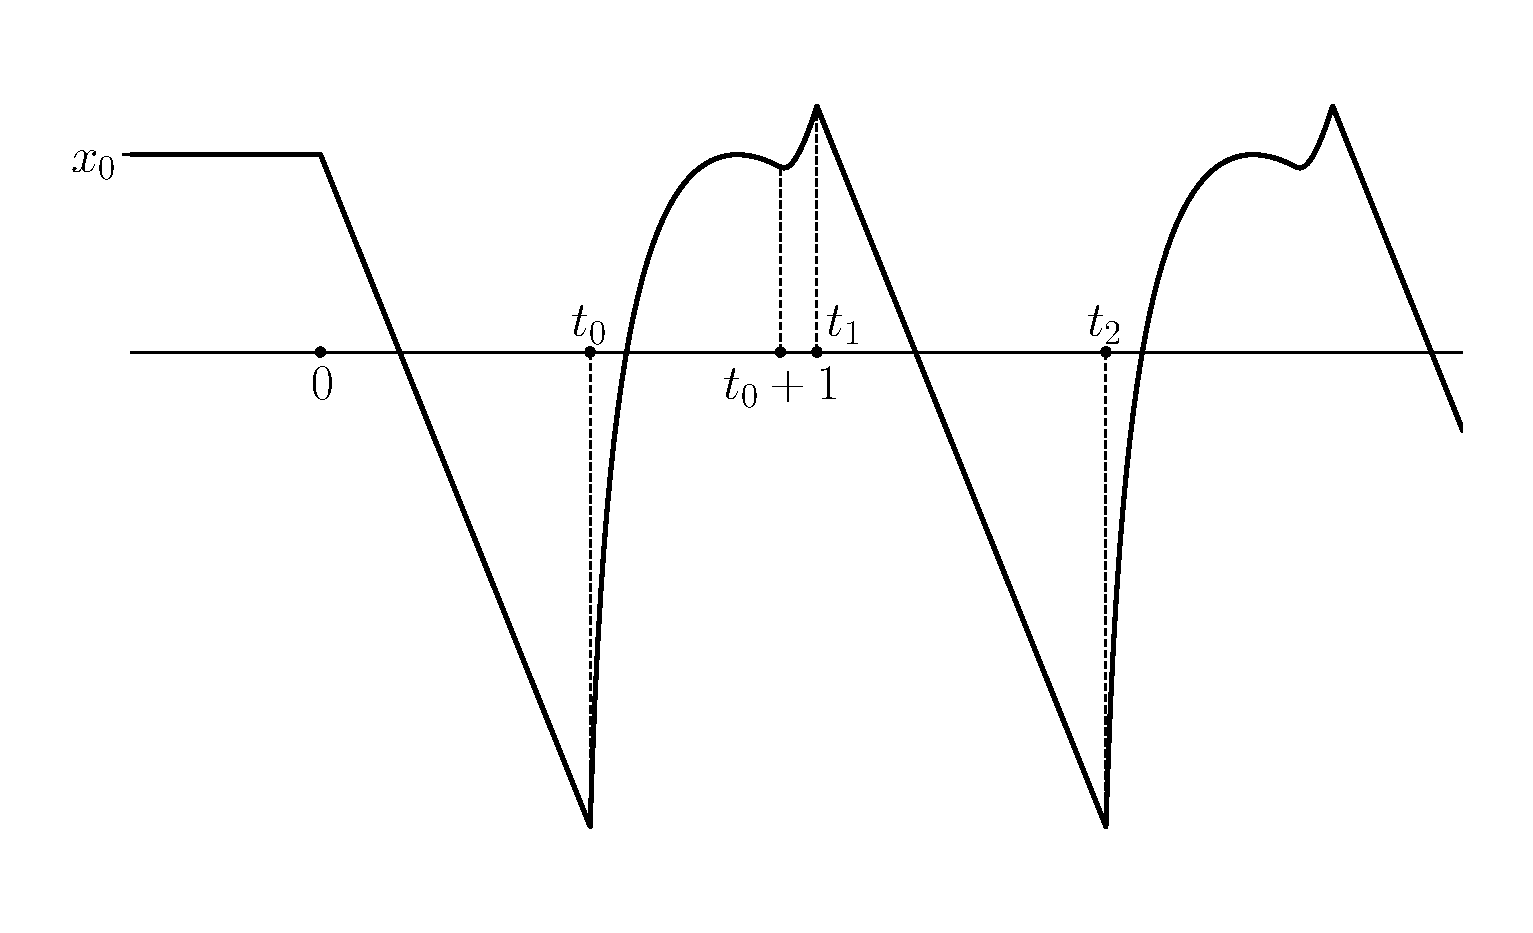
\includegraphics[width=0.7\textwidth]{x_star.eps}
  \captionof{figure}{Периодическое решение $x^{*}(t)$ уравнения \eqref{eq:MG_rele}.}
  \label{fig:x_star:ch1}
\end{figure}


\subsection{Доказательство теоремы о существовании решения релейного уравнения}

Решение уравнения \eqref{eq:MG_rele} строится методом шагов.

Если $t \in [-\sigma_0, 1 - \sigma_0]$, то $x(t - 1) = \phi(t - 1) > 0$, следовательно $x(t)$ отыскивается из начальной задачи Коши
\begin{equation}
    \dot{x} = -\beta, \quad x|_{t = -\sigma_0} = \beta \sigma_0,
\end{equation}
откуда $x(t) = -\beta t$. Аналитический вид решения сохраняется до точки $t = 1$, поскольку в этой точке величина $x(t - 1)$ меняет знак.

На промежутке $t \in [1, 2]$ величина $x(t - 1)$ отрицательна, поэтому решение отыскивается из задачи Коши

\begin{equation}
    \dot{x} = -\beta + \alpha\exp(-\beta(t - 1) - x), \quad x|_{t = 1} = -\beta.
\end{equation}

Эта задача явно интегрируется. После замены $u = e^x$ получаем
\begin{equation*}
	\dot{u} = -\beta u + \alpha e^{-\beta (t - 1)}, \quad u|_{t = 1} = e^{-\beta}.
\end{equation*}
Ищем решение в виде $u(t) = e^{-\beta t} p(t)$, после подстановки в исходное уравнение получаем
\[
\dot{p}(t) = \alpha e^{\beta}, \quad p(t) = 1 + \alpha e^{\beta} (t - 1).
\]
Тогда $u(t) = e^{-\beta t} (\alpha e^{\beta} (t - 1))$, $p(1) = 1$, откуда находим
\begin{equation}
\label{eq:solution_step1:ch1}
    x(t) = -\beta t +\ln(\alpha e^{\beta}(t - 1) + 1).
\end{equation}
%
На следующих шагах решения получаются аналогичным образом, далее детали интегрирования будем опускать.

Следующее изменение аналитического вида решения происходит либо при $t = 3$ (в этот момент аргумент функции $x(t - 1)$ выходит из отрезка $[1, 2]$), либо в точке, где $x(t - 1) = 0$, и величина $x(t - 1)$ второй раз меняет знак.

Проверим, что при ограничении \eqref{eq:cond_alpha1} выполнен второй случай, т.е. корень $t_1$ уравнения $x(t - 1) = 0$, которое с учётом \eqref{eq:solution_step1:ch1}, принимает вид
\begin{equation}
\label{eq:t1_eq}
    -\beta (t - 1) + \ln(\alpha e^{\beta}(t - 2) + 1) = 0,
\end{equation}
существует и лежит на промежутке $(2, 3)$.

В \eqref{eq:t1_eq} обозначим $s = t - 1$, получим
%
$$-\beta s + \ln(\alpha e^{\beta} (s - 1) + 1) = 0$$
%
или, эквивалентно,
%
\begin{equation}
\label{eq:t1_eq2}
e^{\beta s} - \alpha e^{\beta} (s - 1) - 1 = 0.
\end{equation}
Нужно показать, что при условии \eqref{eq:cond_alpha1} существует корень этого уравнения на промежутке $(1, 2)$.

Обозначим левую часть равенства \eqref{eq:t1_eq2} как $H(s) = e^{\beta s} - \alpha e^{\beta} (s - 1) - 1$. Исследуем функцию $H$:
%
\[
H'(s) = \beta e^{\beta s} - \alpha e^{\beta}, \quad H''(s) = \beta^2 e^{\beta s}.
\]
%
Поскольку $H''(s) > 0$, функция $H$ выпукла. Найдём точку минимума $s_{\min}$ из уравнения $H'(s) = 0$:
\[
\beta e^{\beta s} - \alpha e^{\beta} = 0 \Leftrightarrow s = s_{\min} = 1 + \frac{1}{\beta}\ln\frac{\alpha}{\beta}.
\]
%
Поскольку $H(1) = e^{\beta} - 1 > 0$, и при $\alpha > \beta$ верно $s_{\min} > 1$, корень $s = s_* > 1$ уравнения \eqref{eq:t1_eq2} существует тогда и только тогда, когда $H(s_{\min}) \leqslant 0$. Выразим $\alpha$ из этого условия.
%
\[
H(s_{\min}) = \frac{\alpha}{\beta}e^{\beta} - \frac{\alpha}{\beta}e^\beta\ln\frac{\alpha}{\beta} - 1 < 0 \Leftrightarrow \frac{\alpha}{\beta}e^{\beta}\left(1 + \ln\frac{\beta}{\alpha}\right) < 1.
\]

Условие $s_* < 2$ выполняется, если $H(2) < 0$ или $s_{\min} < 2$, что эквивалентно (в первом случае) $\alpha > e^{\beta} - e^{-\beta}$ или (во втором случае) $\alpha < \beta e^{\beta}$.

\begin{proof}
	Утверждение леммы будет доказано в более общем случае в главе \ref{ch:ch2}: в рассуждениях в разделе \ref{ch2:ssect_params} достаточно положить $\tau_* = 2$.
\end{proof}

%\begin{proof}
%Элементарными преобразованиями получаем: 
%\[
%e^{\beta} - e^{-\beta} = \beta e^{\beta} \Leftrightarrow (2\beta - 2) e^{2\beta - 2} = -2e^{-2}.
%\]
%Для отображения $t \mapsto te^t$ каждая точка из интервала $(-1, 0)$ имеет ровно два прообраза, следовательно, возможны две ситуации: $2\beta - 2 = -2$, откуда $\beta = 0$, и $2\beta - 2 = W(-2e^{-2})$, откуда $\beta = \tilde{\beta}$.
%
%Также заметим, что $(e^{\beta} - e^{-\beta})'|_{\beta = 0} > (\beta e^{\beta})'|_{\beta = 0}$, поэтому на промежутке $(0, \tilde{\beta})$ верно неравенство $e^{\beta} - e^{-\beta} > \beta e^{\beta}$. На промежутке $(\tilde{\beta}, +\infty)$ верно обратное неравенство из асимптотических соображений при $\beta \to +\infty$.
%
%Теперь явно выразим $\alpha$ из третьего неравенства в условии леммы.
%\begin{equation*}
%\frac{\alpha}{\beta}e^{\beta}\left(\ln\frac{\beta}{\alpha} + 1\right) < 1\ \Leftrightarrow\ 1 + \ln\dfrac{\beta}{\alpha} < \dfrac{\beta e^{-\beta}}{\alpha}.
%\end{equation*}
%
%Возьмём экспоненту от обеих частей:
%\begin{equation*}
%\dfrac{e\beta}{\alpha} < \exp\dfrac{\beta e^{-\beta}}{\alpha}\ \Leftrightarrow\ \dfrac{-\beta e^{-\beta}}{\alpha}\exp \dfrac{-\beta e^{-\beta}}{\alpha} > -e^{-\beta - 1}\ \Leftrightarrow
%\end{equation*}
%
%\begin{align}
%\label{eq:step3_cond1_expanded:ch1}
%\left[
%\begin{array}{ll}
%    -\frac{\beta e^{-\beta}}{\alpha} > W(-e^{-\beta - 1}),\\
%    -\frac{\beta e^{-\beta}}{\alpha} < W_{-1}(-e^{-\beta - 1}).
%\end{array}
%\right.
%\end{align}
%%
%где $W_{-1}(x)$ --- ветвь функции Ламберта, принимающая значения из промежутка $(-\infty; -1]$.
%
%Однако, второе неравенство соответствует случаю $\dfrac{-\beta e^{-\beta}}{\alpha} < -1$, поскольку $W_{-1}(x) < -1$. Тогда
%\[
%\alpha < \beta e^{-\beta} < \beta,
%\]
%что противоречит условию $\alpha > \beta$.
%
%Значит, совокупность неравенств \eqref{eq:step3_cond1_expanded:ch1} заменяется на единственное неравенство
%\[
%    -\frac{\beta e^{-\beta}}{\alpha} > W(-e^{-\beta - 1}) \Leftrightarrow \alpha > -\dfrac{\beta e^{\beta}}{W(-e^{-\beta - 1})}.
%\]
%%
%Знак неравенства меняется, поскольку $W(-e^{-\beta - 1}) < 0$.
%
%Докажем, что $-\dfrac{\beta e^{-\beta}}{W(-e^{-\beta - 1})} > \beta e^{\beta}$ тогда и только тогда, когда $0 < \beta < \tilde{\beta}$.
%%
%\[
%-\dfrac{\beta e^{\beta}}{W(-e^{-\beta - 1})} > \beta e^{\beta} \Leftrightarrow W(-e^{-\beta - 1}) > -e^{-2\beta} \Leftrightarrow -e^{-\beta - 1} > -e^{-2\beta} \exp(-e^{-2\beta}) \Leftrightarrow
%\]
%%
%\[
%\Leftrightarrow e^{\beta - 1} < \exp(-e^{-2\beta}) \Leftrightarrow \beta - 1 < -e^{-2\beta} \Leftrightarrow \beta e^{\beta} < e^{\beta} - e^{-\beta}.
%\]
%Последнее неравенство верно при $0 < \beta < \tilde{\beta}$, как было доказано выше.
%
%$-\dfrac{\beta e^{-\beta}}{W(-e^{-\beta - 1})} \leqslant e^{\beta} - e^{-\beta}$.
%
%%% !!TODO: завершить доказательство!
%\textbf{Здесь будет завершение доказательства. Оно есть во второй части в более общем случае, может можно сослаться или привести в виде леммы здесь.}
%
%\end{proof}

На отрезке $t \in [2, t_1]$ решение (аналогично предыдущему шагу) отыскивается из задачи Коши 
%
\begin{multline}
    \dot{x} = -\beta + \alpha\exp\bigg(-\beta(t - 1) + \ln(\alpha e^{\beta}(t - 2) + 1) - x\bigg),\\
    x|_{t = 2} = - 2 \beta + \ln(\alpha e^{\beta} + 1),
\end{multline}
%
откуда находим
\begin{equation}
	\label{eq:sol_rele_2}
    x(t) = -\beta t + \ln\left(\frac{\alpha^2}{2}e^{2\beta}(t - 2)^2+\alpha e^{\beta}(t - 1) + 1\right).
\end{equation}
%
После перехода значения $t = t_1$ величина $x(t - 1)$ становится положительной, поэтому уравнение \eqref{eq:MG_rele} вновь принимает вид $\dot{x} = -\beta$. Этот вид сохранится до следующего корня уравнения $x(t - 1) = 0$. Обозначим этот корень как $t_2$. С учётом начальных условий в точке $t_1$, на промежутке $[t_1, t_2]$
\begin{equation}
	\label{eq:sol_rele_3}
	x(t) = -\beta t + \ln\left(\frac{\alpha^2}{2}e^{2\beta}(t_1 - 2)^2 + \alpha e^{\beta}(t_1 - 1) + 1\right).
\end{equation}

Тогда
\begin{equation}
\label{eq:t2}
t_2 = 1 + \dfrac{1}{\beta}\ln\left(\frac{\alpha^2}{2}e^{2\beta}(t - 2)^2 + \alpha e^{\beta}(t - 1) + 1\right).
\end{equation}

Отбросим в \eqref{eq:sol_rele_2} квадратичное слагаемое, получим выпуклую вверх функцию $\tilde{x}(t) = -\beta t + \ln(\alpha e^{\beta} (t - 1) + 1)$, равную нулю (как следует из \eqref{eq:t1_cond_exp}) в точке $t_1 - 1$. Тогда $\tilde{x}(t) > 0$ на промежутке $(t_1 - 1, t_1]$, если $\tilde{x}(t_1) > 0$. Выражая из этого неравенства $\alpha$, с учётом $x(t) \geqslant \tilde{x}(t)$ получим условие \eqref{eq:cond_alpha2}.

Поскольку $x(t) > 0$ на промежутке длины не меньше единицы, последующие шаги построения решения будут совпадать с приведёнными выше, и решение $x(t)$ будет периодическим с периодом $T = t_2 - 1$. Подставляя соответствующее значение $t_2$ в \eqref{eq:t2}, получаем явное значение периода \eqref{eq:T}.

% Отметим, что при $\alpha > \exp(\beta + e^{-\beta})$ условия теоремы выполняются (в этом можно убедиться явной проверкой условий).
% Расписать подробнее

\subsection{Ограничения на параметры уравнения}

Одновременное выполнение условий \eqref{eq:cond_alpha1} и \eqref{eq:cond_alpha2} затруднительно для проверки. Сформулируем достаточное условие, позволяющее легко находить подходящие наборы параметров $\alpha$ и $\beta$.

\begin{theorem}
Пусть параметры $\alpha$, $\beta$ таковы, что $\beta > 0$, $\alpha > \exp(\beta + e^{-\beta})$. Тогда $\alpha$ и $\beta$ удовлетворяют условиям \eqref{eq:cond_alpha1} и \eqref{eq:cond_alpha2}.
\end{theorem}
\begin{proof}
	Следует из утверждения \ref{prop:alpha_greater_phi}, доказанного в главе \ref{ch:ch2}.
\end{proof}

%%%%%%
%%% ОСНОВНОЙ РАЗДЕЛ ПРО АСИМПТОТИКИ
%%%%%%
\section{Асимптотика уравнения Мэки--Гласса}

В данном разделе мы получим следующий результат.

%% !!TODO: Здесь пока нет единственности. Для доказательства единственности надо написать производную Фреше.
\begin{theorem}
    \label{thm:existence}
Пусть параметры $\alpha > \beta > 0$ удовлетворяют условиям \eqref{eq:cond_alpha1} и  \eqref{eq:cond_alpha2}. Тогда существуют такие значения параметров $\sigma_0, p, q$ и такое достаточно большое $\gamma_0$, что при всех $\gamma > \gamma_0$ уравнение \eqref{eq:MG_x} с начальной функцией $\varphi$ из множества \eqref{eq:init_set} обладает периодическим решением $x^*_\gamma(t, \varphi)$ периода $T_{\gamma, \varphi}$, которое удовлетворяет предельным равенствам 
\begin{equation}
\label{eq:lim_x*}
	\lim_{\gamma\to+\infty}\max_{0\leqslant t\leqslant T_{\gamma, \varphi}}|x_{\gamma}^*(t, \phi)-x^*(t)|=0,\quad \lim_{\gamma\to+\infty}T_{\gamma, \varphi} = T,
\end{equation}
где $x^*(t)$ --- решение соответствующего релейного уравнения \eqref{eq:MG_rele} с периодом~$T$, оба предела равномерны по $\varphi \in S$. 
\end{theorem}

\subsection{Общая схема построения асимптотики}
Будем последовательно находить асимптотические формулы по параметру $\gamma \gg 1$ решения $x_{\gamma}^*(t)$ уравнения \eqref{eq:MG_x} методом шагов, опираясь на решение $x^*(t)$ релейного уравнения \eqref{eq:MG_rele}. Техника построения асимптотики сходна с описанной в работах \cite{Kolesov2010, Glyzin2013}.

Назовем \textit{точкой излома} функции $x^*(t)$ точку, в которой она имеет разные односторонние производные. Точки излома следует искать среди точек, в которых функция $x^*(t)$ меняет аналитический вид, то есть среди точек $t = 1$, $2$, $t_1$. Однако, в точке $t = 2$ производные справа и слева совпадают и равны $-\beta+\frac{\alpha e^{\beta}}{\alpha e^{\beta}+1}$, следовательно, $t = 2$ не является точкой излома функции $x^*(t)$. Производные в точке $t = 1$ справа и слева равны соответственно $-\beta$ и $-\beta + \alpha e^\beta$, в точке $t_1$ они равны
%
$$-\beta + \frac{\alpha^2 e^{2\beta}(t_1 - 2) + \alpha e^\beta}{\frac{\alpha^2}{2} e^{2\beta}(t_1-2)^2+\alpha e^{\beta}(t_1 - 1) + 1}$$
%
слева и $-\beta$ справа. 
Таким образом, функция $x^*(t)$ имеет две точки излома: $t = 1$ и $t = t_1$.

Зафиксируем параметр
%
\begin{equation}
	\label{eq:nu_small}
	\nu \in \left( \frac{1}{2}, 1 \right)
\end{equation}
%
и введем малый параметр $\delta$, который следующим образом связан с большим параметром $\gamma$:  
%
\[\delta=\gamma^{-\nu}.\]
%
Параметр $\delta$ имеет смысл радиуса малой окрестности точки излома.

На отрезках 
$[-\sigma_0, 1 - \delta],$ 
$[1 + \delta, 2 - \delta],$ 
$[2 - \delta, 2 + \delta],$ 
$[2 + \delta, t_1 - \delta],$ 
$[t_1 + \delta, t_2 - \delta]$ 
будем искать решение в виде
%
\begin{equation}
    \label{eq:x*gamma_1}
    x^*_\gamma(t, \varphi) = x^*(t) + \Delta(t, \varphi)
\end{equation}
%
и доказывать малость остатка $\Delta$. Для этого определим начальную задачу Коши, которой удовлетворяет остаток $\Delta$. С этой целью подставим \eqref{eq:x*gamma_1} в \eqref{eq:MG_x}, в результате чего получим уравнение
%
\begin{equation*}
    \dot{\Delta} = -\beta + \frac{\alpha\exp(x_{\gamma}^*(t - 1) - x^*(t))}{1 + \exp(\gamma x_{\gamma}^*(t - 1))}e^{-\Delta}-\dot{x}^*.
\end{equation*}
%
Обозначим начало рассматриваемого отрезка через $\tilde{t}$, а значение функции $\Delta$ в этой точке --- через $\tilde{\Delta}$. Для того чтобы найти начальное значение, приравняем значение в точке $\tilde{t}$ функции $x_{\gamma}^*(t)$ на предыдущем и текущем шагах:
%
\[x_{\gamma}^*(\tilde{t}) = x^*(\tilde{t}) + \Delta|_{t=\tilde{t}}.\]
%
Таким образом, $\Delta$ удовлетворяет задаче Коши
\begin{equation}
        \label{eq:task_DeltaAB}
        \dot{\Delta}=A e^{-\Delta} + B,\quad \Delta|_{t=\tilde{t}}=\tilde{\Delta},
\end{equation}
%
\begin{equation}
    \label{AB_eq:x*gamma_1}
\text{где } A = \frac{\alpha\exp(x_{\gamma}^*(t - 1) - x^*(t))}{1+\exp(\gamma x_{\gamma}^*(t - 1))},\, 
B = -\beta-\dot{x}^*,\, 
\tilde{\Delta}=x_{\gamma}^*(\tilde{t}) - x^*(\tilde{t}).
\end{equation}

Для единообразия будем обозначать первую точку излома решения релейной системы
\begin{equation}
	\label{eq:t0:ch1}
	t_0 = 1.
\end{equation}

На отрезках $[t_i - \delta, t_i + \delta],$ $i=0, 1,$ будем предполагать, что решение имеет вид
%
\begin{equation}
    \label{eq:x*gamma_2}
    x^*_\gamma(t) = x^*(t_i) + \frac{1}{\gamma}w_i(\tau)|_{\tau=(t-t_i)\gamma} + \Delta.
\end{equation}
%
Здесь $w_i(\tau)$ --- известные, специальным образом выбранные функции. Подробнее о них будет написано в разделе \ref{subsect:ch1:w_func}. Параметр $\Delta$ --- предстоящий определению остаток, малость которого требуется доказать. Для определения задачи Коши, которой он удовлетворяет, подставим \eqref{eq:x*gamma_2} в \eqref{eq:MG_x} и найдем начальное значение. Получим задачу \eqref{eq:task_DeltaAB} при
\begin{equation}
    \label{AB_eq:x*gamma_2}
    A=\frac{\alpha\exp\big(x_{\gamma}^*(t-1)-x^*(t_i)-\frac{1}{\gamma}w_i(\tau)|_{\tau=(t-t_i)\gamma}\big)}{1+\exp(\gamma x_{\gamma}^*(t-1))},
    \,
    B=-\beta-\frac{dw_i}{d\tau}\Big|_{\tau=(t - t_i)\gamma},
\end{equation}
%
\begin{equation}\label{tilde_eq:x*gamma_2}
    \tilde{t} = t_i - \delta = t_i - \gamma^{-\nu},\quad \tilde{\Delta}=x_{\gamma}^*(\tilde{t}) - x^*(t_i) -\frac{1}{\gamma} w_i(\tau)|_{\tau = -\gamma^{1 - \nu}}.
\end{equation}
%% !!DONE: проверено.

Получаем, что на каждом из рассматриваемых отрезков, остаток $\Delta$ находится из задачи Коши \eqref{eq:task_DeltaAB}. Докажем вспомогательное утверждение.

\begin{lemma}\label{lm:DeltaAB}
Пусть $\tilde{t} \geqslant 0$, $\tilde{\Delta}$ --- известные вещественные числа, $A = A(t),$ $B = B(t)$ --- непрерывные при $t \geq \tilde{t}$ функции, $A(t) > 0$. Тогда решение задачи Коши \eqref{eq:task_DeltaAB} выражается формулой
	\begin{equation}\label{sol_DeltaAB}
	\Delta = J + \ln\Big(1 + \int\limits_{\tilde{t}}^{t} A(s) e^{-J}\,ds \Big),
	\text{ где } J = \tilde{\Delta} + \int\limits_{\tilde{t}}^{t} B(s)\,ds.
	\end{equation}
\end{lemma}
\begin{proof}
    Замена $e^{\Delta}=\theta$ преобразует задачу \eqref{eq:task_DeltaAB} к виду
	%
    \begin{equation}\label{task_theta}
		\dot{\theta}=A+B\theta,\quad\theta|_{t=\tilde{t}}=e^{\tilde{\Delta}}.
    \end{equation}
	%
	Отсюда $\theta=\theta_*(1+\int\limits_{\tilde{t}}^{t}A(s)\theta_*^{-1}ds)$, где $\theta_*(t)=\exp(\tilde{\Delta}+\int\limits_{\tilde{t}}^{t}B(s)ds)$, --- это решение соответствующей однородной задачи $\dot{\theta}=B\theta$.
%	 $\theta|_{t=\tilde{t}}=e^{\tilde{\Delta}}$ --- это функция  
%	Тогда решение задачи \eqref{task_theta} --- это $\theta=\theta_* y$, где $y$ удовлетворяет задаче $\dot{y} = A \theta^{-1}$, $y|_{t=\tilde{t}} = 1$. Отсюда $y = 1 + \int\limits_{\tilde{t}}^{t}A(s)\theta_*^{-1}ds$, следовательно $\theta=\theta_*(1+\int\limits_{\tilde{t}}^{t}A(s)\theta_*^{-1}ds)$.
    
    Тогда $\Delta=\ln\theta=\ln\theta_*+\ln(1+\int\limits_{\tilde{t}}^{t}A(s)\theta_*^{-1}ds),$ откуда следует формула \eqref{sol_DeltaAB}.
\end{proof}
%%!! DONE: проверено.

Из леммы \eqref{lm:DeltaAB} и формул \eqref{AB_eq:x*gamma_1}, \eqref{AB_eq:x*gamma_2}, \eqref{tilde_eq:x*gamma_2} получаем следующие утверждения.
\begin{corollary}\label{corol_Delta_long}
На отрезках $[-\sigma_0, 1 - \delta],$ $[1 + \delta, 2 - \delta],$ $[2 - \delta, 2 + \delta],$ $[2 + \delta, t_1 - \delta],$ $[t_1 + \delta,t_2 - \delta],$ где решение имеет вид \eqref{eq:x*gamma_1}, остаток $\Delta$ определяется формулой
\begin{equation}
    \label{Delta}
    \Delta = J + \ln(1 + I),
\end{equation}
где 
\begin{equation}
    \label{I_long}
    I = \int\limits_{\tilde{t}}^{t}\frac{\alpha\exp(x_{\gamma}^*(s-1)+\beta(s-\tilde{t})-x_{\gamma}^*(\tilde{t}))}{1 + \exp(\gamma x_{\gamma}^*(s-1))} ds,
\end{equation}
%
\begin{equation}\label{eq:J_long}
    J = x_{\gamma}^*(\tilde{t}) - x^*(t) - \beta(t - \tilde{t}),
\end{equation}
%
$\tilde{t}$ --- начальная точка рассматриваемого отрезка.
\end{corollary}
%
\begin{proof}
	Подставим в формулу \eqref{sol_DeltaAB} значения $A$ и $B$ из \eqref{AB_eq:x*gamma_1}. Получим $\Delta = J + \ln(1 + I)$, где
\begin{multline*}
	J = \tilde{\Delta} + \int\limits_{\tilde{t}}^{t}(-\beta - \dot{x}^*(s))ds = x_{\gamma}^*(\tilde{t}) - x^*(\tilde{t}) - \beta(t - \tilde{t}) - x^*(t) + x^*(\tilde{t}) =\\= x_{\gamma}^*(\tilde{t}) - x^*(t) - \beta(t - \tilde{t}),
\end{multline*}
\[
	I = \int\limits_{\tilde{t}}^{t} A e^{-J} \, ds = \int\limits_{\tilde{t}}^{t}\frac{\alpha\exp(x_{\gamma}^*(s-1)+\beta(s-\tilde{t})-x_{\gamma}^*(\tilde{t}))}{1 + \exp(\gamma x_{\gamma}^*(s-1))} ds.
\]
\end{proof}
%
\begin{corollary}\label{corol_Delta_short}
На отрезках $[t_i - \delta, t_i + \delta]$, $i=0, 1$, где решение имеет вид \eqref{eq:x*gamma_2}, остаток $\Delta$ определяется формулой \eqref{Delta} при
 \begin{equation}
    \label{I_point}
   I=\int\limits_{t_i-\delta}^{t}\frac{\alpha\exp\big(x_{\gamma}^*(s-1)+\beta(s-t_i+\delta)-x_{\gamma}^*(t_i-\delta)\big)}{1+\exp(\gamma x_{\gamma}^*(s-1))}ds,
\end{equation}
%
\begin{equation}
    \label{J_point}
    J=x_{\gamma}^*(t_i - \delta) - x^*(t_i) - \beta(t-t_i+\delta) - \frac{1}{\gamma} w_i(\tau)|_{\tau=(t-t_i)\gamma}.
\end{equation}
\end{corollary}
%
\begin{proof}
	Выражая $\tilde{\Delta} = \Delta|_{t = t_i - \delta}$ из \eqref{eq:x*gamma_2}, получаем
\[
	\tilde{\Delta} = x^*_{\gamma}(t_i - \delta) - x^*(t_i) - \frac{1}{\gamma} w_i(\tau)|_{\tau = -\gamma^{1-\nu}}.
\]
Пусть $\tilde{t} = t_i - \delta$. Учитывая $\frac{d}{d\tau} w_i(\tau)|_{\tau = \gamma(t - t_i)} = \frac{d}{dt} \left(\frac{1}{\gamma}w_i(\tau)\right)\Big|_{\tau = \gamma(t - t_i)}$, в формуле \eqref{sol_DeltaAB} получаем
\begin{multline*}
	J = \tilde{\Delta} + \int\limits_{\tilde{t}}^{t} B(s)\,ds = \tilde{\Delta} + \int\limits_{\tilde{t}}^{t}\left(-\beta - \frac{d}{ds} \bigg(\frac{1}{\gamma}w_i(\tau)\bigg)\Big|_{\tau = \gamma(s - t_i)}\right) \,ds =\\= x^*_{\gamma}(t_i - \delta) - x^*(t_i) - \beta(t - t_i - \delta) - \\ - \frac{1}{\gamma} w_i(\tau)|_{\tau = -\gamma^{1-\nu}} - \frac{1}{\gamma}w_i(\tau)|_{\tau = \gamma(t - t_i)} + \frac{1}{\gamma}w_i(\tau)_{\tau = -\gamma^{1 - \nu}} = \\
	= x^*_{\gamma}(t_i - \delta) - x^*(t_i) - \beta(t - t_i - \delta) - \frac{1}{\gamma} w_i(\tau)|_{\tau = \gamma(t - t_i)}.
\end{multline*}
%
По лемме \ref{lm:DeltaAB} получаем, что остаток имеет вид $\Delta = J + \ln(1 + I)$, где 
\[
I = \int\limits_{\tilde{t}}^{t}A(s) e^{-J} ds = \int\limits_{t_i-\delta}^{t}\frac{\alpha\exp\big(x_{\gamma}^*(s-1)+\beta(s-t_i+\delta)-x_{\gamma}^*(t_i-\delta)\big)}{1+\exp(\gamma x_{\gamma}^*(s-1))}ds.
\]
\end{proof}
%% !!DONE: проверено.
%% !!TODO: добавить развёрнутые выкладки.
%
Отметим, что $x_{\gamma}^*(\tilde{t})$ и $x_{\gamma}^*(t_i-\delta)$ в следствиях \ref{corol_Delta_long} и \ref{corol_Delta_short} определяются формулами, полученными на предыдущих шагах.

\subsection{Вспомогательные асимптотические соотношения}

В дальнейшем мы будем пользоваться следующими асимптотическими соотношениями:
\begin{equation}
\label{eq:exp_const}
	e^{\epsilon} = 1 + O(\epsilon) \text{ при } \epsilon \to 0;
\end{equation}
\begin{equation}
\label{eq:exp_linear}
	e^{\epsilon} = 1 + \epsilon + O(\epsilon^2) \text{ при } \epsilon \to 0;
\end{equation}
\begin{equation}
\label{eq:asymp_frac}
	\frac{1}{1 + \varepsilon} = 1 + O(\varepsilon) \text{ при } \epsilon \to 0;
\end{equation}
\begin{equation}
\label{eq:exp_frac}
	\dfrac{1}{1 + e^{x + \epsilon}} = \frac{1}{1 + e^x} + O(\epsilon) \text{ при } \epsilon \to 0.
\end{equation}
\begin{equation}
\label{eq:ln_frac}
\ln(x + \epsilon) = \ln x + \frac{\epsilon}{x} + O(\epsilon^2) \text{ при } \epsilon \to 0, x > 0.
\end{equation}

Соотношения \eqref{eq:exp_const}, \eqref{eq:exp_linear}, \eqref{eq:asymp_frac} очевидны.

Соотношение \eqref{eq:exp_frac} верно и в случае, когда $x$ зависит от $\epsilon$. Действительно,
%
\[
\dfrac{1}{1 + e^x} - \dfrac{1}{1 + e^{x + \epsilon}} = \dfrac{e^x}{(1 + e^x)(1 + e^{x + \epsilon})} \cdot (e^{\epsilon} - 1) = \dfrac{e^x}{(1 + e^x)(1 + e^{x + \epsilon})} \cdot O(\epsilon),
\]
где коэффициент при $O(\epsilon)$ меньше единицы при любых значениях $x$.
%
Соотношение \eqref{eq:ln_frac} доказывается следующим образом:
\[
\ln(x + \epsilon) = \ln x + \ln\left(1 + \frac{\epsilon}{x}\right) = \ln x + \frac{\epsilon}{x} + O(\epsilon^2).
\]
Без дополнительных уточнений оно применимо лишь в случаях, когда $x > 0$ не зависит от $\epsilon$.

\subsection{Асимптотическое поведение в окрестностях точек излома}
\label{subsect:ch1:w_func}

Как было написано выше, для описания асимптотического поведения решения уравнения \eqref{eq:MG_x} в окрестности точек излома $t_i$ введем специальные функции $w_i(t)$. В общем случае их вид зависит от знака $\dot{x}^*(t_i - 1)$. Докажем утверждения о виде данных функций.

\begin{lemma}
\label{lm:w}
	Пусть $x^*(t_i - 1) = 0$, при $t \in [t_i - \delta, t_i + \delta]$ верны соотношения:
	\[ x^*_{\gamma}(t_i - \delta) = x^*(t_i - \delta) + O(\gamma^{-2\nu}), \quad x^*_{\gamma}(t - 1) = x^*(t - 1) + O(\gamma^{-2\nu}).\]
	Тогда решение уравнения \eqref{eq:MG_x} на данном промежутке имеет вид \eqref{eq:x*gamma_2}, где
	
	\[
	w_i(\tau) = -\beta \tau - \dfrac{\alpha e^{-x^*(t_i)}}{\dot{x}^*(t_i - 1)} \ln\left(e^{-\dot{x}^*(t_i - 1)\tau} + 1\right) \quad \text{при} \quad \dot{x}^*(t_i - 1) > 0,
	\]
	\[
	w_i(\tau) = (-\beta + \alpha e^{-x^*(t_i)})\tau - \dfrac{\alpha e^{-x^*(t_i)}}{\dot{x}^*(t_i - 1)} \ln\left(e^{\dot{x}^*(t_i - 1)\tau} + 1\right) \quad \text{при} \quad \dot{x}^*(t_i - 1) < 0,
	\]
	\[
	\Delta = O(\gamma^{-2\nu}).
	\]
\end{lemma}
%
\begin{proof}
	По следствию \ref{corol_Delta_short}, остаток $\Delta$ имеет вид \eqref{Delta}, где $I$ и $J$ определяются формулами \eqref{I_point} и \eqref{J_point} соответственно.
	
	Оценим $I$.
	
	\begin{equation}
	\label{eq:I_point_estimate}
	I = \int\limits_{t_i - \delta}^{t} \dfrac{\alpha \exp(x^*_{\gamma}(s - 1) + \beta(s - t_i + \delta) - x^*_{\gamma}(t_i - \delta))}{1 + \exp(\gamma x^*_{\gamma}(s - 1))}\, ds = \ldots
	\end{equation}
	
	Воспользуемся равенствами
	\[
	x^*(s - 1) = O(\delta), \quad \beta(s - t_i + \delta) = O(\delta), \quad x^*(t_i - \delta) = x^*(t_i) + O(\delta),
	\]
	получим
	\[
	x^*_{\gamma}(s - 1) + \beta(s - t_i + \delta) - x^*_{\gamma}(t_i - \delta) = -x^*(t_i) + O(\delta).
	\]
	Тогда числитель \eqref{eq:I_point_estimate} оценивается как
	\begin{multline*}
	\alpha \exp(x^*_{\gamma}(s - 1) + \beta(s - t_i + \delta) - x^*_{\gamma}(t_i - \delta)) = \alpha \exp(-x^*(t_i) + O(\delta)) =\\= \alpha e^{-x^*(t_i)} \exp(O(\delta)) = \alpha e^{-x^*(t_i)} (1 + O(\delta)).
	\end{multline*}
	
	Преобразуем \eqref{eq:I_point_estimate} в сумму интегралов:
	\[
	\ldots = \int\limits_{t_i - \delta}^{t} \dfrac{\alpha e^{-x^*(t_i)}}{1 + \exp(\gamma x^*_{\gamma}(s - 1))}\, ds + \int\limits_{t_i - \delta}^{t} \dfrac{\alpha e^{-x^*(t_i)} O(\delta)}{1 + \exp(\gamma x^*_{\gamma}(s - 1))} \, ds = \ldots
	\]
	
	Второй интеграл оценим как $O(\delta^2) = O(\gamma^{-2\nu})$. Для оценки первого интеграла воспользуемся равенством
	\[
	x^*_{\gamma}(s - 1) = x^*(s - 1) + O(\gamma^{-2\nu}) = (s - t_i)\dot{x}^*(t_i - 1) + O(\gamma^{-2\nu}).
	\]
	Здесь мы пользуемся тем, что функция $x^*(t)$ разложима по Тейлору до слагаемого второго порядка, а также учитываем $x^*(t_i - 1) = 0$. % Она гладкая везде за исключением изломов.  
	Тогда 
	\[
	\exp(\gamma x^*_{\gamma}(s - 1)) = \exp\left(\gamma(s - t_i)\dot{x}^*(t_i - 1) + O(\gamma^{1 - 2\nu})\right).
	\]
	Из определения \eqref{eq:nu_small} параметра $\nu$, $O(\gamma^{1 - 2\nu})$ мало. Применяя равенство \eqref{eq:exp_frac}, получаем следующую оценку.
	\begin{multline*}
	\dfrac{1}{1 + \exp(\gamma x^*_{\gamma}(s - 1))} = \dfrac{1}{1 + \exp(\gamma (s - t_i) \dot{x}^*(t_i - 1) + O(\gamma^{1 - 2\nu}))} =\\= \dfrac{1}{1 + \exp(\gamma(s - t_i)\dot{x}^*(t_i - 1))} + O(\gamma^{1 - 2\nu}).
	\end{multline*}
	Таким образом,
	\begin{multline*}
	\int\limits_{t_i - \delta}^{t} \dfrac{\alpha e^{-x^*(t_i)} ds}{1 + \exp(\gamma x^*_{\gamma}(s - 1))} = \int\limits_{t_i - \delta}^{t} \left(\dfrac{\alpha e^{-x^*(t_i)}}{1 + \exp(\gamma(s - t_i)\dot{x}^*(t_i - 1))} + O(\gamma^{1 - 2\nu})\right) ds =\\
	= \dfrac{\alpha e^{-x^*(t_i)}}{\gamma \dot{x}^*(t_i - 1)}\ln\left(1 + \exp(-\gamma(s - t_i)\dot{x}^*(t_i - 1))\right)\bigg\vert_{t_i - \delta}^t + O(\gamma^{1 - 3\nu}) = \\
	= \dfrac{\alpha e^{-x^*(t_i)}}{\gamma \dot{x}^*(t_i - 1)}\ln\left(1 + \exp(-\gamma(t - t_i)\dot{x}^*(t_i - 1))\right) -\\- \dfrac{\alpha e^{-x^*(t_i)}}{\gamma \dot{x}^*(t_i - 1)}\ln\left(1 + \exp(\gamma^{1 - \nu}\dot{x}^*(t_i - 1))\right) + O(\gamma^{1 - 3\nu}).
	\end{multline*}
	Если $\dot{x}^*(t_i - 1) < 0$, второе слагаемое экспоненциально мало, и мы получаем оценку 
	\begin{equation}
	\label{eq:I_estimate_dotx_less_0}
	I = \dfrac{\alpha e^{-x^*(t_i)}}{\gamma \dot{x}^*(t_i - 1)}\ln\left(1 + \exp(-\gamma(t - t_i)\dot{x}^*(t_i - 1))\right) + O(\gamma^{1 - 3\nu}).
	\end{equation}
	Если $\dot{x}^*(t_i - 1) > 0$, 
	\begin{multline}
	\dfrac{\alpha e^{-x^*(t_i)}}{\gamma \dot{x}^*(t_i - 1)}\ln\left(1 + \exp(-\gamma(t - t_i)\dot{x}^*(t_i - 1))\right) -\\- \dfrac{\alpha e^{-x^*(t_i)}}{\gamma \dot{x}^*(t_i - 1)}\ln\left(1 + \exp(\gamma^{1 - \nu}\dot{x}^*(t_i - 1))\right) =\\
	= \dfrac{\alpha e^{-x^*(t_i)}}{\gamma \dot{x}^*(t_i - 1)}\ln\left(1 + \exp(\gamma(t - t_i)\dot{x}^*(t_i - 1))\right) - \alpha (t - t_i) e^{-x^*(t_i)} -\\- \dfrac{\alpha e^{-x^*(t_i)}}{\gamma \dot{x}^*(t_i - 1)}\ln\left(1 + \exp(-\gamma^{1 - \nu}\dot{x}^*(t_i - 1))\right) + \alpha \delta e^{-x^*(t_i)}. 
	\end{multline}
	При $\dot{x}^*(t_i - 1) > 0$ третье слагаемое экспоненциально мало, и мы получаем следующую оценку.
	\begin{multline}
		\label{eq:I_estimate_dotx_greater_0}
		I = \dfrac{\alpha e^{-x^*(t_i)}}{\gamma \dot{x}^*(t_i - 1)}\ln\left(1 + \exp(\gamma(t - t_i)\dot{x}^*(t_i - 1))\right) -\\- \alpha (t - t_i - \delta) e^{-x^*(t_i)} + O(\gamma^{1 - 3\nu}).
	\end{multline}
	
	Оценим $J$.
	
	При $\dot{x}^*(t_i - 1) < 0$ на промежутке $[t_i - \delta, t_i]$ уравнение \eqref{eq:MG_rele} имеет вид $\dot{x} = -\beta$, следовательно, 
	\[
	\dot{x}_{\gamma}^*(t_i - \delta) - x^*(t_i) = \dot{x}^*(t_i - \delta) - x^*(t_i) + O(\gamma^{-2\nu}) = -\beta \delta + O(\gamma^{-2\nu}).
	\]
	%
	Подставляя в \eqref{J_point} это равенство и функцию $w(\tau)$ из условия теоремы, получаем
	\begin{multline}
		\label{eq:J_estimate_dotx_less_0}
	J = -\beta \delta + O(\gamma^{-2\nu}) + \beta (t - t_i) - \dfrac{\alpha e^{-x^*(t_i)}}{\gamma \dot{x}^*(t_i - 1)} \ln\left(e^{-\dot{x}^*(t_i - 1)\tau} + 1\right) - \beta(t - t_i - \delta) =\\
	\\= -\dfrac{\alpha e^{-x^*(t_i)}}{\gamma \dot{x}^*(t_i - 1)} \ln\left(e^{-\dot{x}^*(t_i - 1)\tau} + 1\right) + O(\gamma^{-2\nu}).
	\end{multline}
	
	Заметим, что в обоих случаях $I = O(\gamma^{-\nu})$, тогда 
	\begin{equation}
	\label{eq:ln_1_plus_I}
	\ln(1 + I) = I + O(\gamma^{-2\nu}).
	\end{equation}
	
	Подставляя \eqref{eq:I_estimate_dotx_less_0} и \eqref{eq:J_estimate_dotx_less_0} в \eqref{Delta}, получаем
	\[
	\Delta = J + \ln(1 + I) = O(\gamma^{-2\nu}).
	\]
	
	При $\dot{x}^*(t_i - 1) < 0$ получаем
	\begin{multline}
	\label{eq:J_estimate_dotx_greater_0}
	J = x_{\gamma}^*(t_i - \delta) - x^*(t_i) - (-\beta + \alpha e^{-x^*(t_i)})(t - t_i) +\\+ \dfrac{\alpha e^{-x^*(t_i)}}{\gamma \dot{x}^*(t_i - 1)} \ln\left(e^{\dot{x}^*(t_i - 1)\tau} + 1\right) - \beta(t - t_i + \delta) =\\
	= x^*(t_i - \delta) - x^*(t_i) - \alpha e^{-x^*(t_i)}(t - t_i) + \dfrac{\alpha e^{-x^*(t_i)}}{\gamma \dot{x}^*(t_i - 1)} \ln\left(e^{\dot{x}^*(t_i - 1)\tau} + 1\right) -\\- \beta\delta + O(\gamma^{-2\nu}).
	\end{multline}
	
	Подставляя \eqref{eq:I_estimate_dotx_less_0} и \eqref{eq:J_estimate_dotx_less_0} в \eqref{Delta}, и пользуясь оценкой \eqref{eq:ln_1_plus_I}, получаем
	\[
	\Delta = x^*(t_i - \delta) - x^*(t_i) - \beta \delta - \alpha (t - t_i - \delta) e^{-x^*(t_i)} + O(\gamma^{-2\nu}).
	\]
	С учётом 
	\[
	x^*(t_i - \delta) - x^*(t_i) = -\delta\dot{x}(t_i - 0) + O(\delta^2),
	\]
	\[
	\dot{x}(t_i - 0) = \beta + \alpha e^{x^*(t_i - 1) - x^*(t_i)} = \beta + \alpha e^{-x^*(t_i)}
	\]
	получаем
	\[
	\Delta = O(\gamma^{-2\nu}).
	\]
\end{proof}

Сформулируем и докажем утверждение, описывающее асимптотическое поведение введенных функций $w_i(\tau)$ при $\tau\to-\infty$ и $\tau\to+\infty$.
%
\begin{lemma}\label{lm:lem_w_asymp} Верны следующие асимптотические равенства.

Если $\dot{x}(t_i - 1) < 0$,
\begin{equation}
	\label{eq:w0_asymp-}
	w_i(\tau) = -\beta \tau + O(\exp(-\dot{x}^*(t_i - 1) \tau)) \text{ при } \tau \to -\infty,
\end{equation}
\begin{equation}
	\label{eq:w0_asymp+}
	w_i(\tau) = (-\beta + \alpha e^{-x^*(t_i)})\tau + O(\exp(\dot{x}^*(t_i - 1) \tau)) \text{ при } \tau \to +\infty,
\end{equation}
	
Если $\dot{x}(t_i - 1) > 0$,
\begin{equation}
	\label{eq:w1_asymp-}
	w_i(\tau) = (-\beta + \alpha e^{-x^*(t_i)})\tau + O(\exp(\dot{x}^*(t_i - 1) \tau)) \text{ при } \tau \to -\infty,
\end{equation}
\begin{equation}
	\label{eq:w1_asymp+}
	w_i(\tau) = -\beta \tau + O(\exp(-\dot{x}^*(t_i - 1) \tau)) \text{ при } \tau \to +\infty.
\end{equation}
\end{lemma}
\begin{proof}
	При $\dot{x}(t_i - 1) < 0$ верна формула
	\[
	w_i(\tau) = -\beta \tau - \dfrac{\alpha e^{-x^*(t_i)}}{\dot{x}^*(t_i - 1)} \ln\left(e^{-\dot{x}^*(t_i - 1)\tau} + 1\right).
	\]
	
	При $\tau \to -\infty$,
	\[
	\ln\left(e^{-\dot{x}^*(t_i - 1)\tau} + 1\right) = O(\exp(-\dot{x}^*(t_i - 1)\tau)),
	\]
	 откуда следует \eqref{eq:w0_asymp-}.
	 
	При $\tau \to +\infty$,
	\begin{multline*}
	\dfrac{\alpha e^{-x^*(t_i)}}{\dot{x}^*(t_i - 1)} \ln\left(e^{-\dot{x}^*(t_i - 1)\tau} + 1\right) = -\dot{x}^*(t_i - 1)\tau)) = \alpha e^{-x^*(t_i)} \tau + \ln\left(e^{\dot{x}^*(t_i - 1)\tau} + 1\right) =\\
	= \alpha e^{-x^*(t_i)} \tau + O(\exp(\dot{x}^*(t_i - 1) \tau)),
	\end{multline*}
	откуда следует \eqref{eq:w0_asymp+}.
	
	Доказательство формул \eqref{eq:w1_asymp-} и \eqref{eq:w1_asymp+} производится аналогично.
\end{proof}

\begin{remark}
	Коэффициенты при $\tau$ в формулах \eqref{eq:w0_asymp-},\eqref{eq:w0_asymp+},\eqref{eq:w1_asymp-},\eqref{eq:w1_asymp+} совпадают с односторонними производными в точках $x^*(t_i)$ при $i = 0, 1$. 
\end{remark}

Подставляя соответствующие значения $x(t_i),$ $\dot{x}(t_i + 1)$ при $i = 0, 1,$ получаем
\begin{equation}
	\label{eq:w0}
	w_0(\tau)=-\beta \tau+\frac{\alpha e^\beta}{\beta}\ln(e^{\beta\tau}+1),
\end{equation}

% TODO: эту телегу перепроверить
\small
\begin{multline}
	\label{eq:w1}
	w_1(\tau)= -\beta \tau - \frac{\alpha e^\beta(\alpha e^\beta(t_1-2)+1)^2}{(-\beta(\alpha e^\beta(t_1-2)+1)+\alpha e^\beta)(\frac{\alpha^2}{2}e^{2\beta}(t_1-2)^2+\alpha e^{\beta}(t_1-1)+1))}\times
	\\ \times\ln\Bigg(\exp\Big(\beta\tau - \frac{\alpha e^\beta\tau}{\alpha e^\beta(t_1-2)+1}\Big)+1\Bigg).
\end{multline}
\normalsize

%
%\begin{multline}
%	\label{eq:w1}
%	w_1(\tau)=\left(-\beta + \frac{\alpha e^\beta(\alpha e^\beta(t_1-2)+1)}{\frac{\alpha^2}{2}e^{2\beta}(t_1-2)^2+\alpha e^{\beta}(t_1-1) + 1}\right)\tau -\\- \frac{\alpha e^\beta(\alpha e^\beta(t_1-2)+1)^2}{(-\beta(\alpha e^\beta(t_1-2)+1)+\alpha e^\beta)(\frac{\alpha^2}{2}e^{2\beta}(t_1-2)^2+\alpha e^{\beta}(t_1-1)+1))}\times
%	\\ \times\ln\Bigg(\exp\Big(\beta\tau-\frac{\alpha e^\beta\tau}{\alpha e^\beta(t_1-2)+1}\Big)+1\Bigg).
%\end{multline}

\subsection{Построение асимптотики}

Докажем следующую теорему об асимптотическом поведении решения уравнения \eqref{eq:MG_x}.

\begin{theorem}
\label{thm:th_asymp}
Пусть параметры $\alpha,$ $\beta$ удовлетворяют условиям теоремы \ref{thm:existence}, $\alpha > \beta e^{\beta}$, $\gamma \gg 1$, $\delta = \gamma^{-\nu}$, $\nu \in (\frac{1}{2}, 1)$. Уравнение \eqref{eq:MG_x} с произвольной начальной функцией $\varphi$ из класса \eqref{eq:init_set} имеет решение $x_\gamma^*(t, \varphi)$ с асимптотикой
\footnotesize
\begin{equation}
	\label{eq:sol_x*gamma}
	x^*_\gamma(t, \varphi)= 
	\begin{cases}
		- \beta t + O(\gamma^{-1} e^{-\beta \delta \gamma}), & t\in[-\sigma_0, 1 - \delta],\\
		-\beta + \frac{1}{\gamma} w_0(\tau)|_{\tau=(t - 1)\gamma} + O(\gamma^{-2\nu}), & t \in [1 - \delta,1 + \delta]\\
		- \beta t + \ln(\alpha e^{\beta}(t - 1) + 1) + O(\gamma^{-2\nu}) & t\in[1 + \delta, 2]\\
		- \beta t + \ln(\frac{\alpha^2}{2}e^{2 \beta}(t - 2)^2 + \alpha e^{\beta}(t - 1) + 1) + O(\gamma^{-2\nu}) & t \in [2, t_1 - \delta]\\
		- \beta t_1 + \ln(\eta)+\frac{1}{\gamma} w_1(\tau)|_{\tau=(t - t_1)\gamma} + O(\gamma^{-2\nu}) & t\in[t_1 - \delta, t_1  +\delta]\\
		- \beta t + \ln(\eta) + O(\gamma^{-2\nu}) & t \in [t_1 + \delta, t_2 - \delta]
	\end{cases}
\end{equation}
\normalsize
где $\eta=\frac{\alpha^2}{2}e^{2\beta}(t_1 - 2)^2 + \alpha e^{\beta}(t_1 - 1) + 1$.
Асимптотические выражения написаны здесь в предположении $\gamma\to+\infty$.
Все остатки равномерны по $\varphi \in S$ и $t$ из соответствующих промежутков.
\end{theorem}

Для построения асимптотики функции $x_\gamma^*(t)$ последовательно рассмотрим семь отрезков:
$[-\sigma_0, 1 - \delta]$, 
$[1  -\delta, 1 + \delta]$,
$[1 + \delta, 2 - \delta]$,
$[2 - \delta, 2 + \delta]$,
$[2 + \delta, t_1 - \delta]$,
$[t_1 - \delta, t_1 + \delta]$,
$[t_1 + \delta, t_2 - \delta]$.

\subsubsection{Первый шаг построения асимптотики}

Рассмотрим отрезок $[-\sigma_0, 1 - \delta]$. На этом отрезке будем искать решение в виде
%
\begin{equation}
	\label{eq:sol_1}
	x_\gamma^*(t) = -\beta t + \Delta_1,
\end{equation}
%
где $\Delta_1 = \Delta_1(t, \phi)$ --- остаток, порядок малости которого нужно установить. Докажем следующий факт.
%
\begin{lemma}
\label{lm:Delta1}
На отрезке $[-\sigma_0, 1 - \delta]$ функция $x_\gamma^*(t)$ описывается формулой \eqref{eq:sol_1}, причем
%
\[
\Delta_1 = O\left(\gamma^{-1} e^{-\beta\gamma^{1 - \nu}}\right) \text{ при } \gamma \to +\infty.
\]
\end{lemma}
\begin{proof}
Подставим \eqref{eq:sol_1} в \eqref{eq:MG_x}. Сначала рассмотрим отрезок $[-\sigma_0, 1 - \sigma_0]$. Учитывая, что на этом отрезке $x(t - 1) = \varphi(t - 1)$ и $x_\gamma^*(-\sigma_0) = \beta \sigma_0 +\Delta_1|_{t = -\sigma_0} = \beta \sigma_0$, получаем следующую задачу Коши для нахождения $\Delta_1$: 
\begin{equation}
	\label{task_Delta1}
	\dot{\Delta}_1=\frac{\alpha \exp(\varphi(t-1) + \beta t - \Delta_1)}{1 + \exp(\gamma\varphi(t-1))},\quad \Delta_1|_{t = -\beta \sigma_0}=0.
\end{equation}

Дифференциальное уравнение \eqref{task_Delta1} --- уравнение с разделяющимися переменными. Домножим правую и левую части на экспоненту $e^{\Delta_1}$ и проинтегрируем:
%
\[
\int\limits_0^{\Delta_1} e^\Delta d\Delta=\int\limits_{-\sigma_0}^t \frac{\alpha \exp(\varphi(s-1) + \beta s)}{1 + \exp(\gamma\varphi(s - 1))}ds.
\]
%
Интеграл слева равен $e^{\Delta_1} - 1$. Оценим интеграл в правой части.

Экспонента $e^{\beta s}$ в числителе под знаком интеграла ограничена, так как $s$ изменяется на конечном отрезке. Поскольку $\varphi\in S$, верно неравенство
%
\[
\frac{\exp\varphi(s - 1)}{1 + \exp(\gamma\varphi(s - 1))} \leqslant \frac{e^q}{1 + e^{p \gamma}}.
\]
Следовательно, существует положительная константа $C$ (её точное значение неважно) такая, что
\[
\int\limits_{\sigma_0}^t\frac{\alpha\exp\varphi(s-1)-x_0+\beta s}{1+\exp(\gamma\varphi(s-1))}ds\leqslant\frac{C}{1+e^{p \gamma}}.
\]
%
Таким образом, 
\[
e^{\Delta_1}-1=O\Big(\frac{1}{1+e^{p \gamma}}\Big)=O(e^{-p \gamma}).
\]
Отсюда 
\[
\Delta_1=\ln(1+O(e^{-p \gamma}))=O(e^{-p \gamma}) \text{ при }t\in[-\sigma_0, 1 - \sigma_0].
\]
Отметим, что полученная оценка равномерна по $t$ и $\varphi$.

Далее рассмотрим отрезок $[1 - \sigma_0, 1 - \delta]$. Здесь по доказанному выше $x_\gamma^*(t - 1) = -\beta (t-1) + O(e^{-p\gamma}) = -\beta (t-1) + O(e^{-p\gamma})$.

По следствию \eqref{corol_Delta_long}, на этом отрезке остаток имеет вид \eqref{Delta}. Оценим $J$ и $I$.
%
\[
J = x^*_{\gamma}(1 - \sigma_0) - x^*(t) - \beta (t - 1) = -\beta + O(e^{-p\gamma}) + \beta t - \beta(t - 1) = O(e^{-p\gamma}).
\]
%
\[
I = \int\limits_{1 - \sigma_0}^{t}\frac{\alpha\exp(x_{\gamma}^*(s-1)+\beta(s-1)-x_{\gamma}^*(1))}{1 + \exp(\gamma x_{\gamma}^*(s-1))} ds.
\]
Заметим, что
\begin{multline*}
x_{\gamma}^*(s-1)+\beta(s-1)-x_{\gamma}^*(1) = x^*(s - 1) + O(e^{-p\gamma}) + \beta(s - 1) - x^*(1) + O(e^{-p\gamma}) =\\= -\beta(s - 1) + \beta(s - 1) + \beta + O(e^{-p\gamma}) = \beta + O(e^{-p\gamma}),
\end{multline*}
\[
\gamma x^*_{\gamma}(s - 1) = \gamma (x^*(s - 1) + O(e^{-p\gamma})) = -\beta \gamma (s - 1) + O(\gamma e^{-p\gamma}).
\]
Тогда 
\[
I = \int\limits_{1 - \sigma_0}^{t}\frac{\alpha\exp(\beta + O(e^{-p\gamma}))}{1 + \exp(-\beta \gamma (s - 1) + O(\gamma e^{-p\gamma})} ds = \ldots
\]
Воспользуемся асимптотическими равенствами \eqref{eq:exp_const} и \eqref{eq:exp_frac}.
\begin{multline*}
\ldots = \alpha e^{\beta} \int\limits_{1 - \sigma_0}^{t}\left(\frac{1}{1 + \exp(-\beta \gamma (s - 1))} + O(\gamma e^{-p\gamma})\right)(1 + O(e^{-p\gamma})) ds = \\
= \frac{\alpha e^{\beta}}{\beta \gamma} \left(\ln(1 + \exp(\beta \gamma (s - 1)))\right)\bigg\vert_{1 - \sigma_0}^t + O(\gamma e^{-p\gamma}) = \\
= \frac{\alpha e^{\beta}}{\beta \gamma}  \big(\ln(1 + \exp(-\beta \gamma (1 - t))) - \ln(1 + \exp(-\beta \gamma \sigma_0)) \big) + O(\gamma e^{-p\gamma}) = \ldots 
\end{multline*}
%
Первый логарифм оценивается как $O(\exp(-\beta \gamma^{1 - \nu}))$, что асимптотически больше $O(\gamma e^{-p\gamma})$. Таким образом, получаем
\[
I = O(\gamma^{-1} e^{-\beta \gamma^{1 - \nu}}).
\]

Значит,
\begin{equation}
	\label{eq:Delta_step1}
	\Delta_1 = J + \ln(1 + I) = O(\gamma^{-1} e^{-\beta \gamma^{1 - \nu}})
\end{equation}
%
Лемма \ref{lm:Delta1} доказана.

\end{proof}

\subsubsection{Второй шаг построения асимптотики}
Очередной промежуток построения решения --- это $[1 - \delta, 1 + \delta]$. Поскольку на отрезке $[-\sigma_0, 1 - \delta]$ доказана (даже более точная) оценка $x^*_\gamma(t) = x^*(t) + O(\gamma^{-2\nu})$, применима лемма \ref{lm:w} для случая $\dot{x}(t_i - 1) < 0$. Из неё следует, что при $t \in [1 - \delta, 1 + \delta]$ верна оценка
\begin{equation}
	\label{eq:sol_2}
	x_{\gamma}^*(t) = x^*(t) + \frac{1}{\gamma} w_0(\tau)\bigg\vert_{\tau=(t - 1)\gamma} + \Delta_2,
\end{equation}
где $\Delta_2 = O(\gamma^{-2\nu})$. Напомним, функция $w_0(\tau)$ в явном виде описана формулой \ref{eq:w0}.

\subsubsection{Третий шаг построения асимптотики}
Рассмотрим отрезок $[1 + \delta, 2 - \delta]$. Здесь решение отыскивается в виде
\begin{equation}
	\label{eq:sol_3}
	x_\gamma^*(t) = x^*(t) + \Delta_3,
\end{equation}
где $x^*(t) = x_0 - \beta t +\ln(\alpha e^{\beta}(t - 1) + 1),$ $\Delta_3 = \Delta_3(t, \phi)$ --- очередной остаток, предстоящий определению. Докажем следующий факт.

\begin{lemma}
	\label{lm:Delta3}
	На отрезке $[1 + \delta, 2 - \delta]$ функция $x_\gamma^*(t)$ описывается формулой \eqref{eq:sol_3}, причем
	\[
	\Delta_3 = O(\gamma^{-2\nu}) \text{ при } \gamma \to +\infty.
	\]
\end{lemma}
\begin{proof}
Применим следствие \ref{corol_Delta_long} при $\tilde{t} = 1 + \delta$. С учетом асимптотического поведения \eqref{eq:w0_asymp+} функции $w_0(\tau)$ верно
\begin{equation}
\label{eq:x_gamma_t0_delta_step3}
	x_\gamma^*(1 + \delta) = -\beta + \frac{1}{\gamma} w_0(\tau)|_{\tau=\gamma^{1 - \nu}} + O(\gamma^{-2\nu}) = -\beta + (-\beta + \alpha e^\beta)\delta + O(\gamma^{-2\nu}).
\end{equation}

Подставим \eqref{eq:x_gamma_t0_delta_step3} и явный вид $x^*(t)$ в формулу \eqref{eq:J_long}. Получаем:
\small
\begin{multline}
	\label{eq:J_step3}
	J = x_\gamma^*(1 + \delta) - x^*(t) - \beta(t - 1 - \delta) =\\
	= -\beta + (-\beta + \alpha e^\beta)\delta + O(\gamma^{-2\nu}) - 
	(-\beta(t - 2) + \ln(\alpha e^{\beta}(t - 1))) - \beta (t - 1 - \delta) = \\
	 =\alpha e^\beta\delta + O(\gamma^{-2\nu}) - \ln(\alpha e^{\beta}(t - 1) + 1).
\end{multline}
\normalsize

Далее оценим значение $I$. Подставим
%
\begin{multline*}
x^*_{\gamma}(s - 1) + \beta (s - 1 - \delta) - x^*_{\gamma} (1 + \delta) =\\
= x_0 - \beta(s - 1) + \beta(s - 1 - \delta) + \beta + (\beta - \alpha e^{\beta}) \delta + O(\gamma^{-2\nu}) =\\
= \beta - \alpha e^{\beta} \delta + O(\gamma^{-2\nu})
\end{multline*}
%
в формулу \eqref{I_long}. Получим:
\begin{multline*}
	I=\int\limits_{1+\delta}^{t}\frac{\alpha\exp(x_\gamma^*(s-1)+\beta(s-1-\delta)-x_\gamma^*(1+\delta))}{1+\exp(\gamma x_\gamma^*(s-1))} ds =\\
	=\int\limits_{1+\delta}^{t}\frac{\alpha e^{\beta}\exp(-\alpha e^\beta\delta+O(\gamma^{-2\nu}))}{1+\exp( -\beta\gamma (s-1)+O(e^{-\beta\delta\gamma}))} ds,
\end{multline*}
%
что, с учётом асимптотических равенств \eqref{eq:exp_linear} и \eqref{eq:exp_frac}, преобразуется к виду
\begin{multline*}
	I = \int\limits_{1 + \delta}^{t}\Big(\frac{\alpha e^\beta}{1 + \exp(-\beta\gamma(s-1))} + O(\gamma e^{-\beta\delta\gamma})\Big) \cdot \big(1-\alpha e^{\beta} \gamma^{-\nu} + O(\gamma^{-2\nu})\big)ds=\\
	\int\limits_{1+\delta}^{t}\Big(\frac{\alpha e^\beta(1-\alpha e^{\beta}\delta)}{1 + \exp(-\beta\gamma(s-1))} + O(\gamma^{-2\nu})\Big)ds=\\
	= \frac{\alpha e^{\beta}}{\beta\gamma}\big(\ln(e^{\beta\gamma(t - 1)} + 1) - \ln(e^{\beta\gamma^{1-\nu}}+1)\big)(1-\alpha e^{\beta}\delta)+O(\gamma^{-2\nu})=\\
	= \frac{\alpha e^{\beta}}{\beta\gamma}\big(\ln(e^{\beta\gamma(t-1)}(1 + e^{-\beta\gamma(t - 1)})) - \ln(e^{\beta\gamma^{1 - \nu}}(1 + e^{-\beta\gamma^{1-\nu}}))\big)(1-\alpha e^{\beta}\delta)+O(\gamma^{-2\nu}).
\end{multline*}
	
Поскольку $\delta < t - 1$ при $t \in [1 + \delta, 2 - \delta],$ верно неравенство
%
\[-\beta \gamma^{1 - \nu} > - \beta \gamma (t - 1),\]
%
а значит, $e^{-\beta \gamma (t - 1)} = O(e^{-\beta\gamma^{1 - \nu}})$.
Тогда в силу свойств логарифма
%
\begin{multline}
	\label{eq:I_step3}
	I=\frac{\alpha e^{\beta}}{\beta\gamma}\big(\beta\gamma(t-1)-\beta\gamma^{1-\nu}+O(e^{-\beta\gamma^{1-\nu}})\big)(1-\alpha e^{\beta}\delta)+O(\gamma^{-2\nu})=\\
	= \big(\alpha e^{\beta}(t-1)-\alpha e^{\beta}\gamma^{-\nu} + O(\frac{1}{\gamma} e^{-\beta\gamma^{1-\nu}})\big)(1-\alpha e^{\beta}\gamma^{-\nu})+O(\gamma^{-2\nu})=\\
	= \alpha e^{\beta}(t-1)-\alpha e^{\beta}\gamma^{-\nu}-\alpha^2 e^{2\beta}(t-1)\gamma^{-\nu}+O(\gamma^{-2\nu})=\\
	= \alpha e^{\beta}(t-1)-\alpha e^{\beta}\big(\alpha e^{\beta}(t-1)+1\big)\delta+O(\gamma^{-2\nu}).
\end{multline}


Подставляя в \eqref{Delta} формулы \eqref{eq:J_step3}  и \eqref{eq:I_step3}, получим
\begin{multline}
	\label{eq:Delta_step3}
	\Delta_3=J+\ln(1+I)=\alpha e^{\beta}\delta-\ln\big(\alpha e^{\beta}(t-1)+1\big)+O(\gamma^{-2\nu})+\\ \ln\Big(1+\alpha e^{\beta}(t-1)-\alpha e^{\beta}\big(\alpha e^{\beta}(t-1)+1\big)\delta+O(\gamma^{-2\nu})\Big).
\end{multline}

Из справедливости равенства
%
\[\ln(x+\epsilon)-\ln(x) = \frac{\epsilon}{x} + O(\epsilon^2) \quad \text{при } \epsilon \to 0\]
%
следует
\[
\Delta_3 = \alpha e^{\beta}\delta + \frac{-\alpha e^{\beta}(\alpha e^{\beta}(t - 1) + 1)\delta + O(\gamma^{-2\nu})}{\alpha e^{\beta}(t-1)+1} + O(\gamma^{-2\nu}) = O(\gamma^{-2\nu}).
\]
Лемма \ref{lm:Delta3} доказана.
\end{proof}

\subsubsection{Четвёртый шаг построения асимптотики}

Следующий промежуток построения решения --- $[2 - \delta, 2 + \delta]$. Будем искать решение в виде
\begin{equation}
	\label{eq:sol_4}
	x_\gamma^*(t) = x^*(t) + \Delta_4, \text{ где } 
\end{equation}
\small
\begin{equation}
\label{eq:x_star_4_step}
x^*(t) = 
\begin{cases}
x_0 - \beta t + \ln(\alpha e^{\beta}(t - 1) + 1), & t \in [2 - \delta, 2],\\
x_0 -\beta t + \ln(\frac{\alpha^2}{2} e^{2\beta}(t - 2)^2 + \alpha e^{\beta}(t - 1) + 1), & t \in [2,2 + \delta],
\end{cases}
\end{equation}
\normalsize
$\Delta_4$ --- предстоящий определению остаток.

\begin{lemma}
\label{lem_Delta4}
На отрезке $[2 - \delta, 2 + \delta]$ функция $x_\gamma^*(t)$ описывается формулой \eqref{eq:sol_4}, причем
\[
	\Delta_4 = O(\gamma^{-2\nu}) \text{ при } \gamma \to +\infty.
\]
\end{lemma}

\begin{proof}

Применим следствие \ref{corol_Delta_long}. Оценим величину $J$. В данном случае $\tilde{t} = 2 - \delta$, тогда формула \eqref{eq:J_long} принимает вид
%
\[
J = x_\gamma^*(2 - \delta) - x^*(t) - \beta(t - 2 + \delta).
\]
%
Подставляя сюда формулы \eqref{eq:x_star_4_step}, получим
%
\[
	J = \ln(\alpha e^{\beta} (1 - \delta) + 1) - \ln(\alpha e^{\beta}(t - 1) + 1) + O(\gamma^{-2\nu})
\]
при $t\in [2 - \delta, 2]$ и
%
\[
	J = \ln(\alpha e^{\beta} (1 - \delta) + 1) - \ln \left(\frac{\alpha^2}{2}e^{2\beta}(t-2)^2  + \alpha e^{\beta}(t-1)+1 \right) + O(\gamma^{-2\nu})
\]
при $t\in [2, 2 + \delta].$
%
Из равенства \eqref{eq:ln_frac} и соотношения $(t - 2)^2 = O(\gamma^{-2\nu})$ следует
\begin{multline*}
\ln \left(\frac{\alpha^2}{2} e^{2\beta} (t - 2)^2  + \alpha e^{\beta}(t - 1) + 1 \right) =\\= \ln (\alpha e^{\beta}(t - 1) + 1 + O(\gamma^{-2\nu})) = \ln (\alpha e^{\beta}(t - 1) + 1) + O(\gamma^{-2\nu}).
\end{multline*}
%
Таким образом, на отрезке $[2 - \delta, 2 + \delta]$ получаем
%
\[
J = \ln(\alpha e^{\beta} (1 - \delta) + 1) - \ln(\alpha e^{\beta}(t - 1) + 1) + O(\gamma^{-2\nu})
\]
%
Далее, из равенства \eqref{eq:ln_frac} и соотношения $t - 2 = O(\delta)$ следуют равенства
\[
 \ln(\alpha e^{\beta} (1 - \delta) + 1) = \ln(\alpha e^{\beta} + 1) - \frac{\alpha e^{\beta}\delta}{\alpha e^{\beta} + 1} + O(\gamma^{-2\nu}),
\]
\[
\ln(\alpha e^{\beta} (t - 1) + 1) = \ln(\alpha e^{\beta} + 1) + \frac{\alpha e^{\beta} (t - 2)}{\alpha e^{\beta} + 1} + O(\gamma^{-2\nu}),
\]
откуда
\begin{equation}
\label{eq:J_step4}
J = -\frac{\alpha e^{\beta} (t - 2 + \delta)}{\alpha e^{\beta} + 1} + O(\gamma^{-2\nu}).
\end{equation}

Оценим величину $I$.
%
\begin{multline*}
x_\gamma^*(2 - \delta) = -2\beta + \beta \delta + \ln(\alpha e^{\beta}(1 - \delta) + 1) + \Delta_3 =\\
= -2 \beta + \beta \delta + \ln(\alpha e^{\beta} + 1) - \frac{\alpha e^{\beta}\delta}{\alpha e^\beta + 1} +\Delta_3.
\end{multline*}
%
Подставим это выражение, \eqref{eq:sol_2} и $\tilde{t} = 2 - \delta$ в формулу \eqref{I_long}, и после элементарных преобразований получим

\begin{comment}
\[
I = \int\limits_{\tilde{t}}^{t}\frac{\alpha\exp(x_\gamma^*(s-1)+\beta(s-\tilde{t})-x_\gamma^*(\tilde{t}))}{1+\exp(\gamma x_\gamma^*(s-1))}ds = 
\]
\[
= \int\limits_{2-\delta}^{t}\frac{\alpha\exp(-\beta+\frac1\gamma w_0|_{\tau=(t-2)\gamma}+\Delta_2+\beta(s-2+\delta)-x^*_\gamma(2-\delta))}{1+\exp(-\beta\gamma+ w_0|_{\tau=(t-2)\gamma}+\gamma\Delta_2)}ds=
\]
\[
= \int\limits_{2-\delta}^{t}\frac{\alpha\exp(-\beta+\frac1\gamma (-\beta \tau+\frac{\alpha e^\beta}{\beta}\ln(e^{\beta\tau}+1))|_{\tau=(t-2)\gamma}+\Delta_2+\frac1\gamma\beta\tau+\beta\delta-x^*_\gamma(2-\delta))}{1+\exp(-\beta\gamma+ (-\beta \tau+\frac{\alpha e^\beta}{\beta}\ln(e^{\beta\tau}+1))|_{\tau=(t-2)\gamma}+\gamma\Delta_2)}ds=
\]
\[
= \int\limits_{2-\delta}^{t}\frac{\alpha\exp(-\beta+ \frac{\alpha e^\beta}{\beta\gamma}\ln(e^{\beta\tau}+1)|_{\tau=(t-2)\gamma}+\Delta_2+\beta\delta-(-2\beta+\beta\delta+\ln(\alpha e^{\beta}+1)-\frac{\alpha e^{\beta}\delta}{\alpha e^\beta+1} +\Delta_3))}{1+\exp(-\beta\gamma+ (-\beta \tau+\frac{\alpha e^\beta}{\beta}\ln(e^{\beta\tau}+1))|_{\tau=(t-2)\gamma}+\gamma\Delta_2)}ds=
\]
\end{comment}

\begin{multline*}
I = \frac{\alpha e^\beta}{\alpha e^{\beta}+1}\exp\Big(\frac{\alpha e^{\beta}\delta}{\alpha e^\beta+1}\Big) \times
\\
\times\int\limits_{2-\delta}^{t}\frac{\exp( \frac{\alpha e^\beta}{\beta\gamma}\ln(e^{\beta\tau}+1)|_{\tau=(s-2)\gamma} +O(\gamma^{-2\nu}))}{1+\exp(-\beta\gamma+ (-\beta \tau+\frac{\alpha e^\beta}{\beta}\ln(e^{\beta\tau}+1))|_{\tau=(s-2)\gamma}+O(\gamma^{1 - 2\nu}))}ds
\end{multline*}
%
Перейдём под знаком интеграла к новой переменной $\tau=(s-2)\gamma$:
\small
\begin{equation}
	\label{eq:I_step4}
	I = \frac{\alpha e^\beta}{\gamma(\alpha e^{\beta}+1)}\exp\Big(\frac{\alpha e^{\beta}\delta}{\alpha e^\beta+1}\Big)
	\int\limits_{-\gamma \delta}^{\gamma (t - 2)}\frac{\exp( \frac{\alpha e^\beta}{\beta\gamma}\ln(e^{\beta\tau} + 1) +O(\gamma^{-2\nu}))}{1 + e^{-\beta(\gamma+\tau)}(e^{\beta\tau} + 1)^\frac{\alpha e^\beta}{\beta}\exp(O(\gamma^{1-2\nu}))} d\tau.
\end{equation}
\normalsize

При $t \in [2 - \delta, 2]$ верно $\tau < 0$, поэтому логарифм в числителе ограничен: $0 < \ln(e^{\beta\tau} + 1) < \ln 2$. Отсюда следует, что аргумент экспоненты в числителе под знаком интеграла --- малая величина. Тогда, применяя асимптотическую формулу \eqref{eq:exp_const}, получаем
\begin{equation}
	\label{eq:exp_numerat}
	\exp\Big( \frac{\alpha e^\beta}{\beta \gamma}\ln(e^{\beta\tau}+1) +O(\gamma^{-2\nu})\Big) = 1 + O(\gamma^{-1}).
\end{equation}

Поскольку $-\beta(\gamma + \tau) \in [-\beta\gamma, -\beta\gamma(1-\gamma^{-\nu})]$, второе слагаемое в знаменателе под знаком интеграла мало. Тогда применяя асимптотическую формулу \eqref{eq:asymp_frac} и используя формулу \eqref{eq:exp_numerat}, получаем
\begin{multline*}
	I=\frac{\alpha e^\beta}{\gamma(\alpha e^{\beta}+1)}\exp\Big(\frac{\alpha e^{\beta}\delta}{\alpha e^\beta+1}\Big)
	\int\limits_{-\gamma\delta}^{\gamma(t-2)}(1+O(\gamma^{-1}))d\tau
	=\\
	=\frac{\alpha e^\beta}{\gamma(\alpha e^{\beta}+1)}\exp\Big(\frac{\alpha e^{\beta}\delta}{\alpha e^\beta+1}\Big)(\gamma(t - 2) + \gamma\delta + O(\delta))
	=\\
	=\frac{\alpha e^\beta}{(\alpha e^{\beta}+1)}\exp\Big(\frac{\alpha e^{\beta}\delta}{\alpha e^\beta+1}\Big)(t-2+\delta+O(\delta\gamma^{-1})).
\end{multline*}
Используя разложение \eqref{eq:exp_linear}, получаем
\begin{multline}
	\label{eq:I_step4_1}
	I = \frac{\alpha e^\beta}{(\alpha e^{\beta} + 1)}\Big(1 + \frac{\alpha e^{\beta}\delta}{\alpha e^\beta+1} + O(\delta^2)\Big)(t-2+\delta+O(\delta\gamma^{-1})) = \\
	= \frac{\alpha e^\beta(t-2+\delta)}{\alpha e^\beta+1}+O(\gamma^{-2\nu}).
\end{multline}

Теперь, подставляя в \eqref{Delta} значения $J$ и $I$ из формул \eqref{eq:J_step4} и \eqref{eq:I_step4_1}, получаем необходимую малость $\Delta$ на отрезке $[2 - \delta, 2]$.
%
\begin{multline}
	\label{Delta_step4}
	\Delta=-\frac{\alpha e^\beta(t-2+\delta)}{\alpha e^\beta+1}+O(\gamma^{-2\nu}) + \\
	+ \ln\Big(1+\frac{\alpha e^\beta(t-2+\delta)}{\alpha e^\beta+1}+O(\gamma^{-2\nu})\Big)=O(\gamma^{-2\nu}).
\end{multline}


Теперь рассмотрим $I$ при $t \in [2, 2 + \delta]$. Разобьём интеграл \eqref{eq:I_step4} на два интеграла по отрезкам $[-\delta\gamma, 0]$ и  $[0, \gamma (t - 2)]$. Первый интеграл имеет асимптотику \eqref{eq:I_step4_1} при подстановке $t = 2$. Тогда формулу \eqref{eq:I_step4} можно переписать в виде
\small
\begin{multline}
	\label{eq:I_step4_2}
	I=\frac{\alpha e^\beta\delta}{\alpha e^\beta+1}+O(\gamma^{-2\nu})+
	\\
	\frac{\alpha e^\beta}{\gamma(\alpha e^{\beta}+1)}\exp\Big(\frac{\alpha e^{\beta}\delta}{\alpha e^\beta+1}\Big)
	\int\limits_{0}^{\gamma(t - 2)}\frac{\exp( \frac{\alpha e^\beta\tau}{\gamma}+\frac{\alpha e^\beta}{\beta\gamma}\ln(1+e^{-\beta\tau}) +O(\gamma^{-2\nu}))}{1+e^{-\beta\gamma+(\alpha e^\beta-\beta)\tau}(1+e^{-\beta\tau})^\frac{\alpha e^\beta}{\beta}\exp(O(\gamma^{1 - 2\nu}))}d\tau.
\end{multline}
\normalsize
Здесь $\tau \in [0,\delta\gamma]$, поэтому $\frac{\tau}{\gamma} = O(\delta)$, логарифм $\ln(1 + e^{-\beta\tau})$ ограничен, его значения лежат в промежутке $[0,\ln 2]$. Как и в предыдущем случае под знаком интеграла в числителе получаем экспоненту с малым аргументом, поэтому к числителю применима асимптотическая формула \eqref{eq:exp_linear}. В знаменателе показатель экспоненты $-\beta\gamma + (\alpha e^\beta - \beta) \tau \in [-\beta\gamma, -\gamma(\beta + (\alpha e^\beta - \beta) \gamma^{-\nu})]$. Отсюда и из ограниченности $(1 + e^{-\beta\tau})^\frac{\alpha e^\beta}{\beta}$ получаем малость второго слагаемого в знаменателе под знаком интеграла. Как в предыдущем случае вычисления $I$, применяя формулу \eqref{eq:exp_const}, получаем представление
%
\small
\begin{multline*}
	I=\frac{\alpha e^\beta\delta}{\alpha e^\beta+1}+O(\gamma^{-2\nu})+
	\frac{\alpha e^\beta}{\gamma(\alpha e^{\beta}+1)}\exp\Big(\frac{\alpha e^{\beta}\delta}{\alpha e^\beta+1}\Big)
	\int\limits_{0}^{(t-2)\gamma}(1+O(\gamma^{-\nu}))d\tau=
	% \\
	% \frac{\alpha e^\beta\delta}{\alpha e^\beta+1}+O(\gamma^{-2\nu})+
	% \frac{\alpha e^\beta}{\gamma(\alpha e^{\beta}+1)}\exp\Big(\frac{\alpha e^{\beta}\delta}{\alpha e^\beta+1}\Big)\big(
	% (t-2)\gamma+O(\gamma^{1-2\nu})\big)=
	\\
	\frac{\alpha e^\beta\delta}{\alpha e^\beta+1}+O(\gamma^{-2\nu})+
	\frac{\alpha e^\beta}{\alpha e^{\beta}+1}\exp\Big(\frac{\alpha e^{\beta}\delta}{\alpha e^\beta+1}\Big)\big(
	t-2+O(\gamma^{-2\nu})\big)=
	\\
	\frac{\alpha e^\beta\delta}{\alpha e^\beta+1}+O(\gamma^{-2\nu})+
	\frac{\alpha e^\beta}{\alpha e^{\beta}+1}\Big(1+\frac{\alpha e^{\beta}\delta}{\alpha e^\beta+1}+O(\delta^2)\Big)\big(
	t-2+O(\gamma^{-2\nu})\big)=
	\\
	% \frac{\alpha e^\beta\delta}{\alpha e^\beta+1}+O(\gamma^{-2\nu})+
	% \frac{\alpha e^\beta}{\alpha e^{\beta}+1}\big(
	% t-2+O(\gamma^{-2\nu})\big)=
	% \\
	\frac{\alpha e^\beta}{\alpha e^{\beta}+1}(
	t-2+\delta)+O(\gamma^{-2\nu}),
\end{multline*}
\normalsize
что совпадает с асимптотикой для $I$, полученной на отрезке $[2 - \delta, 2]$.
Отсюда следует формула \eqref{Delta_step4}. 

Лемма \ref{lem_Delta4} доказана.

\end{proof}

%TODO: возможно, здесь что-то можно сократить. Пока не буду писать здесь.


\subsubsection{Пятый шаг построения асимптотики}

Найдем асимптотику решения при $t \in [2 + \delta, t_1 - \delta]$. Будем искать решение в виде
\begin{equation}
	\label{eq:sol_5}
	x_\gamma^*(t) = x^*(t) + \Delta_5,
\end{equation}
%
где 
\[x^*(t) = x_0 - \beta t + \ln\left(\frac{\alpha^2}{2} e^{2\beta} (t - 2)^2 + \alpha e^{\beta}(t - 1) + 1 \right),\]
а остаток $\Delta_5$ предстоит оценить. Докажем следующую лемму.
%
\begin{lemma}
\label{lem_Delta5}
На отрезке $[2 + \delta, t_1 - \delta]$ функция $x_\gamma^*(t)$ описывается формулой \eqref{eq:sol_5}, причем
\[
\Delta_5 = O(\gamma^{-2\nu}) \text{ при } \gamma \to +\infty.
\]
\end{lemma}
\begin{proof}
%
Применим следствие \ref{corol_Delta_long}. В данном случае $\tilde{t} = 2 + \delta$.
Тогда
%
\[
J = x_\gamma^*(2 + \delta) - x^*(t) - \beta(t - 2 - \delta).
\]
%
Здесь
\begin{multline}
	\label{x*gamma_tilde_step4}
	x_\gamma^*(2 + \delta) = x^*(2 + \delta) + \Delta_4 = \\
	= -2 \beta - \beta \delta + \ln\left(\frac{\alpha^2}{2} e^{2\beta} \delta^2 + \alpha e^{\beta} (1 + \delta) + 1 \right) + \Delta_4,
\end{multline}
%
\[ % TODO: проверить, нет ли тут минуса
x^*(t) = \beta(t_0 - 1) - \beta t + \ln\left(\frac{\alpha^2}{2} e^{2\beta}(t - 2)^2 + \alpha e^{\beta}(t - 1) + 1\right),
\]
%
тогда
\begin{multline}
	\label{J_step5}
	J = \ln\left(\frac{\alpha^2}{2}e^{2\beta}\delta^2 + \alpha e^{\beta}(\delta + 1) + 1 \right) -\\- \ln\Big(\frac{\alpha^2}{2}e^{2\beta}(t - 2)^2+\alpha e^{\beta}(t - 1) + 1 \Big) + \Delta_4=
	\\
	-\ln\left(\frac{\frac{\alpha^2}{2}e^{2\beta}(t - 2)^2+\alpha e^{\beta}(t - 1) + 1}{\alpha e^{\beta}(\delta + 1) + 1 + O(\gamma^{-2\nu})}\right) + O(\gamma^{-2\nu}).
\end{multline}

Теперь найдём
\begin{equation*}
	I = \int\limits_{2 + \delta}^{t} \frac{\alpha \exp(x_\gamma^*(s - 1) + \beta(s - 2 - \delta) - x_\gamma^*(2 + \delta))}{1 + \exp(\gamma x_\gamma^*(s - 1))}ds.
\end{equation*}
Учитывая формулы \eqref{x*gamma_tilde_step4} и
%
\[
x_\gamma^*(s-1) = -\beta (s - 1) + \ln(\alpha e^{\beta}(s - 2) + 1) + \Delta_3,
\]
%
получим
%
\small
\begin{equation*}
	I = \int\limits_{2 + \delta}^{t}\frac{\alpha e^\beta \exp\left( \ln(\alpha e^{\beta}(s - 2) + 1) - \ln(\frac{\alpha^2}{2} e^{2\beta} \delta^2 + \alpha e^{\beta}(1 + \delta) + 1) + \Delta_3 - \Delta_4 \right)}{1 + \exp\left(\gamma x^*(s-1)  +\gamma\Delta_3\right)} ds.
\end{equation*}
\normalsize

% Дальше тонкий момент, который надо осознать и расписать
Заметим, что $s \in [2 + \delta, t] \subset [2 + \delta, t_1 - \delta]$, значит, $s - 1 \in [2 + \delta, t_1 - 1 - \delta]$, где $t_1 - 1$ --- это корень уравнения $x^*(t)=0$, причем функция $x^*(t)$ меняет в точке $t = t_1 - 1$ знак с отрицательного на положительный. Из выпуклости вверх функции $x^*(t)$ на отрезке $[1, 2]$ и условия $x^*(t) > 0$ следует, что $\dot{x}(t_1 - 1) > 0$, т.~е. решение пересекает нулевое значение трансверсально.

 %Условие $\alpha > \beta e^{\beta}$ гарантирует трансверсальность пересечения нуля, т.к.
%
%\begin{multline*}
%\dot{x}(t_1 - 1) = -\beta + \alpha \exp(x(t_1 - 2) - x(t_1 - 1)) =\\= -\beta + \alpha \exp(x(t_1 - 2)) > %-\beta + \alpha e^{-\beta} > 0.
%\end{multline*}
%
Таким образом, здесь $x^*(s - 1) < -C \delta = -C \gamma^{-\nu}$, где $C > 0$ --- константа, точное значение которой не важно. Тогда $\exp(\gamma x^*(s - 1))=O(\exp(-C \gamma^{1 - \nu}))$. Учитывая выше сказанное и вынося коэффициент перед знаком интеграла, получим  
\begin{equation*}
	I=\frac{\alpha e^\beta}
	{\frac{\alpha^2}{2}e^{2\beta}\delta^2+\alpha e^{\beta}(1+\delta)+1}
	%
	\int\limits_{2 + \delta}^{t}
	%
	\frac{\big(\alpha e^{\beta}(s-2)+1\big)\exp\big(O(\gamma^{-2\nu})\big)}
	%
	{1+O\big(\exp({-r\gamma^{1-\nu}})\big) \exp\big(O(\gamma^{1-2\nu})\big)}
	%
	ds. 
\end{equation*}
Отметим, что показатель $1-2\nu<0$ в силу выбора $\nu$. Используем асимптотические формулы \eqref{eq:exp_const}, \eqref{eq:asymp_frac} при $\epsilon \to 0$:
%
\begin{multline*}
	I=\frac{\alpha e^\beta}
	{\frac{\alpha^2}{2}e^{2\beta}\delta^2+\alpha e^{\beta}(1+\delta)+1}
	\int\limits_{2 + \delta}^{t}
	\big(\alpha e^{\beta}(s-2)+1\big)\big(1+O(\gamma^{-2\nu})\big)
	ds=
	\\
	= \frac{\frac{\alpha^2}{2} e^{2\beta}(t-2)^2+\alpha e^\beta(t-2-\delta)+O(\gamma^{-2\nu})}
	{\alpha e^{\beta}(1+\delta)+1+O(\gamma^{-2\nu})}.
\end{multline*}
%
Тогда
\begin{multline}
	\Delta_5=J+\ln(1+I)=
	-\ln\Big(\frac{\frac{\alpha^2}{2}e^{2\beta}(t-2)^2+\alpha e^{\beta}(t-1)+1}{\alpha e^{\beta}(\delta+1)+1+O(\gamma^{-2\nu})}\Big)+O(\gamma^{-2\nu})
	+
	\\
	\ln\Big(\frac{\frac{\alpha^2}{2} e^{2\beta}(t-2)^2+\alpha e^\beta(t - 1)+1+O(\gamma^{-2\nu})}
	{\alpha e^{\beta}(1+\delta)+1+O(\gamma^{-2\nu})}\Big)=O(\gamma^{-2\nu}).
\end{multline}        

Лемма \ref{lem_Delta5} доказана.

\end{proof}

\subsubsection{Шестой шаг построения асимптотики}

Очередной промежуток построения решения --- это $[t_1-\delta, t_1+\delta]$. Поскольку $x^*_{\gamma}(t_1 - \delta) = x^*(t_1) + \Delta_5$, $x^*_{\gamma}(t - 1) = x^*(t - 1) + \Delta_3$, где $\Delta_5 = O(\gamma^{-2\nu})$, $\Delta_3 = O(\gamma^{-2\nu})$, на данном промежутке применима лемма \ref{lm:w}. Таким образом, решение имеет вид
\begin{equation}
	\label{eq:sol_6}
	x_{\gamma}^*(t) = x^*(t) + \frac{1}{\gamma} w_1(\tau)\bigg\vert_{\tau=(t - t_1)\gamma} + \Delta_6,
\end{equation}
где $\Delta_6 = O(\gamma^{-2\nu})$.


\subsubsection{Седьмой шаг построения асимптотики}

На заключительном этапе построения рассмотрим отрезок $[t_1+\delta, t_2-\delta]$. Здесь будем искать решение в виде
\begin{equation}
	\label{eq:sol_7}
	x_\gamma^*(t) = x^*(t) + \Delta_7.
\end{equation}

Докажем следующий факт
\begin{lemma}
\label{lm:Delta_7}
На отрезке $[t_1 + \delta, t_2 - \delta]$ функция $x_\gamma^*(t)$ описывается формулой \eqref{eq:sol_7}, причем
\[
\Delta_7 = O(\gamma^{- 2\nu})\text{ при }\gamma\to\infty.
\]
\end{lemma}
\begin{proof}
Применим следствие \ref{corol_Delta_long}.
Оценим интеграл
%
\begin{equation*}
	I = \int \limits_{t_1+\delta}^{t}\frac{\alpha\exp(x_\gamma^*(s - 1) + \beta(s - t_1 - \delta) - x_\gamma^*(t_1 + \delta))}{1  +\exp(\gamma x_\gamma^*(s - 1))}ds.
\end{equation*}
%
На рассматриваемом отрезке $x_\gamma^*(s - 1) > 0$, причем существует константа $C > 0$ (точное значение которой не важно), такая, что $x_\gamma^*(s-1) > C\delta.$

Действительно, данная оценка верна на отрезке $[t_1 - 1 + \delta, t_1]$, поскольку пересечение нуля в точке $t_1 - 1$ трансверсально. Далее, из \eqref{eq:sol_6} следует, что $x^*_{\gamma}(t_1) = x^*(t_1) + O(\gamma^{-1})$. На отрезке $[t_1, t_2]$ верно $\dot{x}^*(t) = -\beta$, $\dot{x}^*_\gamma(t) > -\beta$, поскольку второе слагаемое уравнения \eqref{eq:MG_x} положительно. Значит, разность $x^*_{\gamma}(t) - x^*(t)$ на отрезке $[t_1, t_2]$ возрастает. Тогда
%
\[
x^*_{\gamma}(t) - x^*(t) > x^*_{\gamma}(t_1) - x^*(t_1) = O(\gamma^{-1}).
\]
%
Следовательно,
%
\[
x^*_{\gamma}(t) > x^*(t) + O(\gamma^{-1}) > x^*(t_2 - 1 - \delta) + O(\gamma^{-1}) = \beta\delta + O(\gamma^{-1}),
\]
откуда следует существование $C > 0$.
	
Тогда
\begin{equation}
	\label{I_step7}
	I = \int\limits_{t_1+\delta}^{t} O\left(\frac{1}{1 + e^{C \delta \gamma}}\right) ds = O\left(\frac{1}{1 + e^{C \delta \gamma}}\right) = O(e^{-C\delta\gamma}).
\end{equation}

Поскольку здесь
\[
x_\gamma^*(t_1+\delta) = x^*(t_1) + \frac{1}{\gamma} w_1(\tau)\bigg\vert_{\tau=\delta\gamma} + \Delta_6,
\]
то в силу асимптотического поведения \eqref{eq:w1_asymp+} функции $w_1$ получаем
\begin{multline*}
	J = x_\gamma^*(t_1 + \delta) - x^*(t) - \beta(t - t_1 - \delta) =\\
	x^*(t_1) + \frac{1}{\gamma} (-\beta\tau + O(\exp(-\dot{x}^*(t_1 - 1) \tau)))\bigg\vert|_{\tau = \delta\gamma} + O(\gamma^{-2\nu}) - x^*(t) - \beta(t - t_1 - \delta) =\\
	= (x^*(t_1) - x(t)) - \beta \delta - \beta(t - t_1 - \delta) + O(\gamma^{-2\nu}) = O(\gamma^{-2\nu}),
\end{multline*}
поскольку $x^*(t_1) - x^*(t) = \beta (t - t_1)$.

Тогда $\Delta = J + \ln(1 + I) = O(\gamma^{-2\nu})$.
	
\end{proof}

Теорема \ref{thm:th_asymp} доказана.

\subsection{Доказательство существования периодического решения}

Из асимптотических соотношений \eqref{eq:sol_x*gamma} следует, что на промежутке $[1 - \delta; t_2 - \delta]$ длины $T$ верно равенство
\[
x_\gamma^*(t, \varphi) = x^*(t) + O(\gamma^{-2\nu}),
\]
где остаток равномерен по $\varphi \in S$.
% \end{proof}
Отсюда,
\[
\max\limits_{0 \leqslant t \leqslant t_2 - \delta}|x_\gamma^*(t, \varphi) - x^*(t)| = O(\gamma^{-2\nu}).
\]

Далее, уточним параметры $\sigma_0, p, q$, характеризующие множество $S = S(\sigma_0, p, q)$ начальных функций. Пусть $\sigma_0$ таково, что
%
\[
0 < \beta \sigma_0 < \max\limits_{t \in [1, T + 1]} x^*(t).
\]
%
Тогда уравнение $x^*_\gamma(t - \sigma_0, \varphi) = \beta \sigma_0$, по крайней мере для достаточно больших $\gamma$, имеет корень $T_{\gamma, \varphi}$, больший $t_1$ и меньший $t_2 - \delta$.

Из доказательства теоремы \ref{thm:relay} известно, что на промежутке $[t_1 - 1, t_2 - 1]$ длины, большей единицы, верно $x^*(t) > 0$. Тогда на промежутке $[T_{\gamma, \varphi} - 1, T_{\gamma, \varphi}]$ верно $x^*_{\gamma}(t, \varphi) > 0$.

Теперь можно зафиксировать
\[
p = \frac{1}{2}\min\limits_{t \in [T - 1 - \sigma_0, T - \sigma_0]} x^*(t), \ q > \max\limits_{t \in [T - 1 - \sigma_0, T - \sigma_0]} x^*(t)
\]
и все рассуждения в доказательстве асимптотических формул проводить в этих предположениях.

Определим оператор $\Pi_{\gamma}: S(\sigma_0, p, q) \to C[-1-\sigma_0; -\sigma_0]$:
\begin{equation}
	\Pi_{\gamma}(\varphi): t \mapsto x^*_{\gamma}(t + T_{\gamma, \varphi}, \varphi).
\end{equation}

Из оценок \eqref{eq:u_bound} и \eqref{eq:dot_u_bound} следует, что множество функций $\{\Pi_{\gamma}(\varphi)\, | \, \varphi \in S\}$ равномерно ограничено вместе со своими производными, оно является равностепенно непрерывным, откуда из теоремы Арцела следует вполне непрерывность оператора $\Pi_{\gamma}$. Таким образом, компактный оператор $\Pi_{\gamma}$ преобразует замкнутое, ограниченное, выпуклое множество $S(\sigma_0, p, q)$ в себя. В соответствие с принципом Шаудера \cite{Krasnov1975}, отсюда следует существование неподвижной точки $\varphi^*$ этого оператора, которой соответствует периодическое решение $x^*_\gamma(t, \varphi^*)$ с найденной асимптотикой \eqref{eq:sol_x*gamma}. Условия \eqref{eq:lim_x*} следуют из асимптотических соотношений.

%%% Выводы %%%
\subsection{Выводы к главе 1}

В работе проводится построение асимптотики уравнения \eqref{eq:MG_norm} по степеням малого параметра $\gamma^{-\nu}$, где показатель нелинейности $\gamma$ полагается большим параметром. Данное предположение оправдано тем, что в оригинальной статье \cite{Mackey1977} приводятся значения (после нормировки на запаздывание) $\alpha$, $\beta$ порядка единицы и $\gamma = 10$. Численное моделирование показывает, что для таких значений предельный цикл уравнения \eqref{eq:MG_norm} оказывается достаточно близок к циклу предельного при $\gamma \to +\infty$ уравнения \eqref{eq:MG_rele}. Подобное предположение используется в статьях \cite{Bartha2021, Krisztin2020}, а также в работах, посвящённых генным сетям (см., например, \cite{Volokitin2004}), где возникает аналогичная нелинейность.

Отметим, что похожий подход к построению асимптотики решения применяется в статьях \cite{Kolesov2010, Kolesov1997, Glyzin2013} и других работах тех же авторов.

В работах \cite{Bartha2021,Krisztin2020} также доказывается близость решения уравнения (\ref{eq:MG_norm}) и решения его предельной версии при $\gamma\to+\infty$. В статье \cite{Krisztin2020} рассматривается случай близких значений параметров $\alpha$ и $\beta$, а в \cite{Bartha2021} случай большого $\alpha$  по сравнению с $\beta$, а именно случай 
\begin{equation}
	\label{cond_Bartha}
	\alpha>\max\{\beta e^\beta, e^\beta-e^{-\beta}\}.
\end{equation}
Заметим, что ограничения \eqref{cond_Bartha} и \eqref{eq:cond_alpha1}, \eqref{eq:cond_alpha2} описывают схожие области, однако неравенство \eqref{cond_Bartha} оказывается более сильным. 
В работах \cite{Bartha2021,Krisztin2020} доказывается сходимость решения уравнения \eqref{eq:MG_norm} к решению предельного при $\gamma\to+\infty$ со ссылкой на общий результат, изложенный в XIV главе книги \cite{Diekmann1995}.
В качестве отличия настоящей работы от \cite{Bartha2021} отметим точную асимптотическую оценку разности решений уравнений \eqref{eq:MG_x} и \eqref{eq:MG_rele} (аналогичная пара уравнений, рассмотренным в  работах \cite{Bartha2021,Krisztin2020}, но после экспоненциальной замены).



           % Глава 1
\chapter{Периодические режимы в виде дискретной бегущей волны в полносвязной системе генераторов Мэки--Гласса}\label{ch:ch2}

В данной главе рассматривается полносвязная цепь генераторов Мэки--Гласса:
\begin{equation}
	\label{eq:system_full_generators}
	\dfrac{d V_{j}}{dt}=- bV_{j} + \dfrac{ac\left(V_{j}(t - \tau) + \sum\limits_{k = 0, k\neq j}^{m}V_{k}(t)\right)}{1 + \left(c\left(V_{j}(t - \tau) + \sum\limits_{k = 0, k\neq j}^{m}V_{k}(t)\right)\right)^{\gamma}}, \quad j=0,1,\ldots,m.
\end{equation}

Коротко опишем план главы. В разделе \ref{sec:ch2/sect1} формулируется постановка задачи, описывается механизм построения дискретных бегущих волн. В разделе \ref{sec:ch2/sect2} анализируется вспомогательное уравнение со множеством запаздываний, доказывается существование периодического решения. В разделе \ref{sec:ch2/sect3} доказывается существование периодического решения системы в виде дискретной бегущей волны. В разделе \ref{sec:ch2/sect4} приводятся результаты численного эксперимента.

\section{Постановка задачи}\label{sec:ch2/sect1}

Сделаем в \eqref{eq:system_full_generators} подстановки
%
\begin{equation}
	\label{eq:mg_norm}
	\beta = b \tau, \ \alpha = ac \tau, \ t = \tau \tilde{t}, V_j(t) = \dfrac{1}{c}u_j\left(\dfrac{t}{\tau}\right) = \dfrac{1}{c}u_j(\tilde{t}).
\end{equation}
%
Получим:
%
\begin{equation*}
	\frac{d}{dt} \left(\dfrac{1}{c}u_j\left(\dfrac{t}{\tau}\right)\right)= -\dfrac{\beta}{\tau c}u_j(\tilde{t}) + \dfrac{\alpha}{\tau c}\dfrac{u_j(\tilde{t} - 1) + \sum\limits_{k = 0, k\neq j}^m u_k(\tilde{t})}{1 + \left(u_j(\tilde{t} - 1) + \sum\limits_{k = 0, k\neq j}^m u_k(\tilde{t})\right)^{\gamma}}
\end{equation*}
%
\begin{equation*}
	\frac{1}{\tau} \dot{u}_j(\tilde{t}) = -\dfrac{\beta}{\tau}u_j(\tilde{t}) + \dfrac{\alpha}{\tau}\dfrac{u_j(\tilde{t} - 1) + \sum\limits_{k = 0, k\neq j}^m u_k(\tilde{t})}{1 + \left(u_j(\tilde{t} - 1) + \sum\limits_{k = 0, k\neq j}^m u_k(\tilde{t})\right)^{\gamma}}
\end{equation*}
%
Для удобства будем писать $t$ вместо $\tilde{t}$, получим:
%
\begin{equation}
	\label{eq:mg_full_renormed}
	\dot{u}_j(t) = -\beta u_j(t) + \dfrac{\alpha \left(u_j(t - 1) + \sum\limits_{k = 0, k\neq j}^m u_k(t)\right)}{1 + \left(u_j(t - 1) + \sum\limits_{k = 0, k\neq j}^m u_k(t)\right)^{\gamma}}
\end{equation}
%
Будем считать $\gamma \gg 1$ большим параметром. Пусть 
%
\begin{equation}
\label{eq:relay_function_F}
F(w)\stackrel{\text{def}}{=}\lim\limits_{\gamma\rightarrow+\infty} \frac{1}{1+w^\gamma}=\left\lbrace\begin{array}{cl}
	1, & 0<w<1 \\
	\frac{1}{2}, & w=1, \\
	0, & w>1.
\end{array}\right.
\end{equation}
%
Тогда при $\gamma \to +\infty$ система \eqref{eq:mg_full_renormed} примет вид
%
\begin{equation}
\label{eq:system_relay}
\dot{u}_j=-\beta u_j+\alpha\left(u_j(t-1)+ \sum\limits_{k=0, k\neq j}^{m} u_{k}(t)\right)F\left(u_j(t-1)+\sum\limits_{k=0, k\neq j}^{m} u_{k}(t)\right).
\end{equation}

Решением системы \eqref{eq:system_relay} в форме \emph{дискретной бегущей волны} будем называть решение вида
%
\begin{equation}
	\label{eq:discrete_wave}
	u_j(t) = u(t + k_j\Delta),   
\end{equation}
где $\{k_0, k_1, \ldots, l_m\}$ --- перестановка номеров $\{0, 1, \ldots, m\}$, $u(t)$ --- некоторая функция, $\Delta > 0$ --- сдвиг.

Пусть $u(t)$ --- периодическая функция с периодом $T$. В уравнении \eqref{eq:system_relay} для фиксированного $j$ сделаем подстановку \eqref{eq:discrete_wave} и выполним сдвиг времени $t + k_j \Delta \mapsto t$. Получим
%
\small
\begin{equation}
	\label{eq:mg_relay_0}
	\dot{u} = -\beta u+\alpha\left(u(t-1)+ \sum_{s=0,s\neq j}^{m}u(t+(k_s-k_j)\Delta)\right)F\left(u(t-1)+ \sum_{s=0, s\neq j}^{m}u(t+(k_s-k_j)\Delta)\right).
\end{equation}
\normalsize

Заметим, что множество значений $\{(k_s - k_j) \mod (m + 1) \ | \ s \neq j\}$ совпадает с множеством $\{1, 2, \ldots, m\}$. Предположим, что сдвиг $\Delta$ таков, что величина $(m + 1) \Delta$ кратна периоду $T$, т.~е. существует число $p \in \mathbb{N}$ такое, что
%
\begin{equation}
	\label{eq:period_equation}
	pT = (m + 1)\Delta
\end{equation}
%
Из этого предположения следует равенство сумм
%
\begin{equation}
	\label{eq:shift_sum_equality}
	\sum\limits_{s=0, s\neq j}^{m}u(t+(k_s-k_j)\Delta)=\sum\limits_{s=1}^{m}u(t-s\Delta).
\end{equation}
%
Подставляя \eqref{eq:shift_sum_equality} в \eqref{eq:mg_relay_0}, сведём последнее к не зависящему от $j$ виду:
%
\begin{equation}
	\label{eq:mg_relay_1}
	\dot{u}=-\beta u+\alpha\left(u(t-1)+ \sum_{s=1}^{m}u(t-s\Delta)\right)F\left(u(t-1)+ \sum_{s=1}^{m}u(t-s\Delta)\right).
\end{equation}
%
Таким образом, задача решения системы \eqref{eq:system_relay} сводится к поиску $T$-периодического решения уравнения \eqref{eq:mg_relay_1} и параметра $\Delta > 0$, при некотором $p \in \mathbb{N}$ удовлетворяющего условию \eqref{eq:period_equation}. Уравнение \eqref{eq:mg_relay_1} в дальнейшем будем называть \emph{вспомогательным уравнением}.

%%%
%%% АНАЛИЗ ВСПОМОГАТЕЛЬНОГО УРАВНЕНИЯ
%%%
\section{Анализ вспомогательного уравнения}\label{sec:ch2/sect2}

\subsection{Запаздывания}

В уравнении \eqref{eq:mg_relay_1} функция $u(t)$ входит с запаздываниями $1$, $\Delta$, $2\Delta$, \dots, $m\Delta$. Упорядочим запаздывания: пусть
$$\tau_0 < \tau_1 < \tau_2 < \ldots < \tau_m,$$
где множество $\{\tau_0, \tau_1, \ldots, \tau_m\}$ совпадает с множеством $\{1, \Delta, 2\Delta, \ldots, m\Delta\}$.

Тогда уравнение \eqref{eq:mg_relay_1} можно переписать в виде
\begin{equation}
	\label{eq:mg_relay_tau}
	\dot{u}=-\beta u+\alpha\left(\sum_{s=0}^{m}u(t-\tau_s)\right)F\left(\sum_{s=0}^{m}u(t-\tau_s)\right)
\end{equation}
%
Проведём в \eqref{eq:mg_relay_tau} нормировку времени, делающее наименьшее запаздывание равным единице. Пусть
%
\begin{equation*}
	\tilde{t} = \frac{t}{\tau_0}, \ u(t) = \tilde{u}\left(\frac{t}{\tau_0}\right), \ \alpha = \frac{\tilde{\alpha}}{\tau_0}, \ \beta = \frac{\tilde{\beta}}{\tau_0}, \ \tilde{\tau}_s = \frac{\tau_s}{\tau_0} \ (s = 0, 1, \ldots, m).
\end{equation*}
%
Получаем
%
\begin{equation*}
	\frac{d}{dt} \tilde{u}\left(\frac{t}{\tau_0}\right) = -\frac{\beta}{\tau_0} \tilde{u}(\tilde{t}) + \frac{\tilde{\alpha}}{\tau_0} \left(\sum_{s=0}^{m}\tilde{u}(\tilde{t}-\tilde{\tau}_s)\right) F \left(\sum_{s=0}^{m}\tilde{u}(\tilde{t}-\tilde{\tau}_s)\right).
\end{equation*}
%
Домножим на $\tau_0$ и для удобства уберём <<тильды>> над обозначениями. Получим в точности уравнение \eqref{eq:mg_relay_tau}, в котором изменились только запаздывания $\tau_s$.
%
Введём обозначение для суммы функций $u(t)$ с задаздываниями $\tau_s$:
%
\begin{equation*}
	w(t) = \sum\limits_{s = 0}^m u(t - \tau_s).
\end{equation*}
%
Тогда уравнение \eqref{eq:mg_relay_tau} примет компактный вид
%
\begin{equation}
	\label{eq:mg_relay_w}
	\dot{u}=-\beta u+\alpha w(t) F(w(t)).
\end{equation}

\subsection{Множество начальных функций}

Множество $S$ начальных функций определим на промежутке длины наибольшего запаздывания: 
%
\begin{equation}
	\label{eq:mg_init_set}
	S = \{\varphi\in C[-\tau_{m},0]:\  \varphi(t)>1 \text{ при } t\in[-\tau_{m},0),\ \varphi(0)=u_0\},
\end{equation}
%
где параметр $u_0 > 1$.

\subsection{Точки переключения}

\emph{Точками переключения} будем называть точки, в которых правая часть уравнения \eqref{eq:mg_relay_w} изменяет аналитический вид. К ним относятся точки следующих двух типов.
\begin{enumerate}
	\item[a)] Корни уравнения $w(t) = 1$. Будем обозначать их $t_k$.
	В точках $t_k$ происходит <<переключение>> релейного множителя $F(w(t))$.
	\item[б)] Точки переключения вида $t_k + \tau_s$ при условии $w(t_k + \tau_s) < 1$. При таких значениях $t$ релейный множитель $F(w(t)) = 1$, а значит, правая часть уравнения \eqref{eq:mg_relay_w} имеет вид
	%
	\begin{equation*}
		-\beta u+\alpha \big(u(t-\tau_0)+u(t-\tau_1)+\ldots+u(t-\tau_{m})\big),
	\end{equation*}
	%
	в точке $t_k + \tau_s$ слагаемое $u(t - \tau_s)$ меняет аналитический вид.
\end{enumerate}

Будем искать периодическое решение уравнения \eqref{eq:mg_relay_w} \emph{с минимальным числом точек переключения}.

\begin{theorem}
	\label{prop:switching_points_2}
	Периодический режим уравнения \eqref{eq:mg_relay_w} имеет не менее двух точек переключения $t_0, t_1$ типа а).
\end{theorem}
\begin{proof}
	Ввиду периодичности решения, число точек переключения должно быть чётным. Докажем, что оно не может быть равно нулю. Из условия на начальные функции \eqref{eq:mg_init_set} следует, что $w(t) > 1$ по крайней мере на промежутке $[0; \tau_m]$, следовательно, решение находится из задачи Коши
	%
	\begin{equation*}
		\dot{u} = -\beta u, \quad u(0) = u_0.
	\end{equation*}
	%
	Её решение имеет вид
	%
	\begin{equation*}
		u(t) = u_0 e^{-\beta t},
	\end{equation*}
	%
	что не является периодической функцией, следовательно, хотя бы одна точка переключения должна быть.
\end{proof}


\subsection{Результат для вспомогательного уравнения}\label{sec:ch2/sect2/subsect_aux_result}

Введем обозначения:
%
\begin{equation*}
	A = \sum_{i=0}^{m}e^{\beta \tau_{i}}=e^\beta+e^{\beta \tau_1}+\ldots+e^{\beta \tau_{m}},
\end{equation*}
\begin{equation*}
	\tau_* = \min\{2,\tau_1\}=\left\lbrace\begin{array}{cl}
		\min\{2,1/\Delta\}, & \text{ если } \Delta<1,
		\\
		\min\{2,\Delta\}, & \text{ если } \Delta>1,
	\end{array}\right.
\end{equation*}
\begin{equation*}
	s_* = t_1-t_0.
\end{equation*}

%%%%%%%%%%%%%
%% Теорема %%
%%%%%%%%%%%%%
\begin{theorem}
	\label{thm:mg_auxiliary_main}
	Пусть параметры $\alpha, \beta$ и величина $\tau_*$ удовлетворяют ограничениям
	
	\begin{equation}
		\label{eq:cond_thm1}
		\frac{\alpha}{\beta}e^{\beta}\left(\ln\left(\frac{\beta}{\alpha}\right)+1\right) < 1,
		\quad
		\alpha > \beta.
	\end{equation}
	
	\begin{equation}
		\label{eq:cond_thm2}
		e^{\beta \tau_*}-1 \leqslant \alpha e^\beta(\tau_*-1)
		\quad\text{или}\quad
		0 < \frac{1}{\beta}\ln\frac{\alpha}{\beta}\leqslant\tau_*-1,
	\end{equation}
	
	\begin{equation}
		\label{eq:cond_th_w>1_t_1+1}
		e^{-\beta s_*}(e^{-\beta}+\alpha s_*)>1
	\end{equation}
	
	\begin{equation}
		\label{eq:cond_hair_hair_01}
		\frac{\alpha^2}{2}e^\beta(s_*-1)^2+\alpha s_*>\frac{e^{\beta \tau_k}-1}{\sum_{i=0}^{k-1}e^{\beta \tau_i}},\text{ если } s_*\leqslant \tau_k-\tau_{k-1},\quad k=1,\ldots,m,
	\end{equation}
	\begin{equation}
		\label{eq:cond_hair_hair_02}
		\frac{\alpha^2}{2}e^\beta(s_*-1)^2+\alpha s_*>\frac{e^{\beta (s_*+\tau_{k-1})}-1}{\sum_{i=0}^{k-1}e^{\beta \tau_i}},\text{ если } s_* > \tau_k-\tau_{k-1},\quad k=1,\ldots,m,
	\end{equation}
	\begin{equation}
		\label{eq:cond_hair_hair_1}
		\frac{\alpha^2}{2}e^\beta( s_*-1)^2+\alpha s_*>\frac{(e^{\beta s_*}-\alpha s_*)e^{\beta \tau_k}-1}{\sum_{i=0}^{k-1}e^{\beta \tau_i}},\quad k=1,\ldots,m.
	\end{equation}
	Тогда решение уравнения \eqref{eq:mg_relay_w} при любой  начальной функции из множества \eqref{eq:mg_init_set} совпадает с одной и той же периодической функцией. Назовем эту функцию $u_*$, а ее период $T$. Справедливо следующее.
	
	1. Функция $u_*(t)$ обладает наименьшим числом переключений на периоде: $t_0$, $t_0+1$, $t_1$. При этом 
	%
	\begin{equation*}
		t_0=\frac{1}{\beta}\ln(u_0 A),
	\end{equation*}
	\begin{equation}
		e^{\beta s_*} - 1=\alpha e^{\beta}(s_* - 1), \quad s_* \in (1, \tau_*).
	\end{equation}
	
	2. Функция $u_*(t)$ и период $T$ имеют следующий явный вид: 
	%
	\small
	\begin{equation}
		\label{eq:u_star}
		u_*(t)=
		\begin{cases}
			u_0 e^{-\beta t}(\alpha A(t-t_0)+1) & \text{ при } t\in[t_0,t_0+1].
			\\
			u_0 e^{-\beta t}\left(\frac{\alpha^2}{2}Ae^{\beta}(t-t_0-1)^2+\alpha A(t-t_0)+1\right) & \text{ при } t\in[t_0+1,t_1],
			\\
			u_0 e^{-\beta t}\left(\frac{\alpha^2}{2}Ae^{\beta}(t_1-t_0-1)^2+\alpha A(t_1-t_0)+1\right) & \text{ при } t\in[t_1,t_0+T].
		\end{cases}
	\end{equation}
	\normalsize
	%
	\[
	u_*(t+T)\equiv u_*(t),
	\]
	%
	\begin{equation}
		\label{eq:mg_period_T}
		T = \dfrac{1}{\beta}\ln\left( \frac{\alpha^2}{2}Ae^{\beta}(t_1-t_0-1)^2+\alpha A(t_1-t_0)+1\right). 
	\end{equation}
\end{theorem}

Схематичный график функции $u_*$ изображен на рисунке \ref{fig:u_star}.
%
\begin{figure}[h]
	\label{fig:u_star}
	\centering
	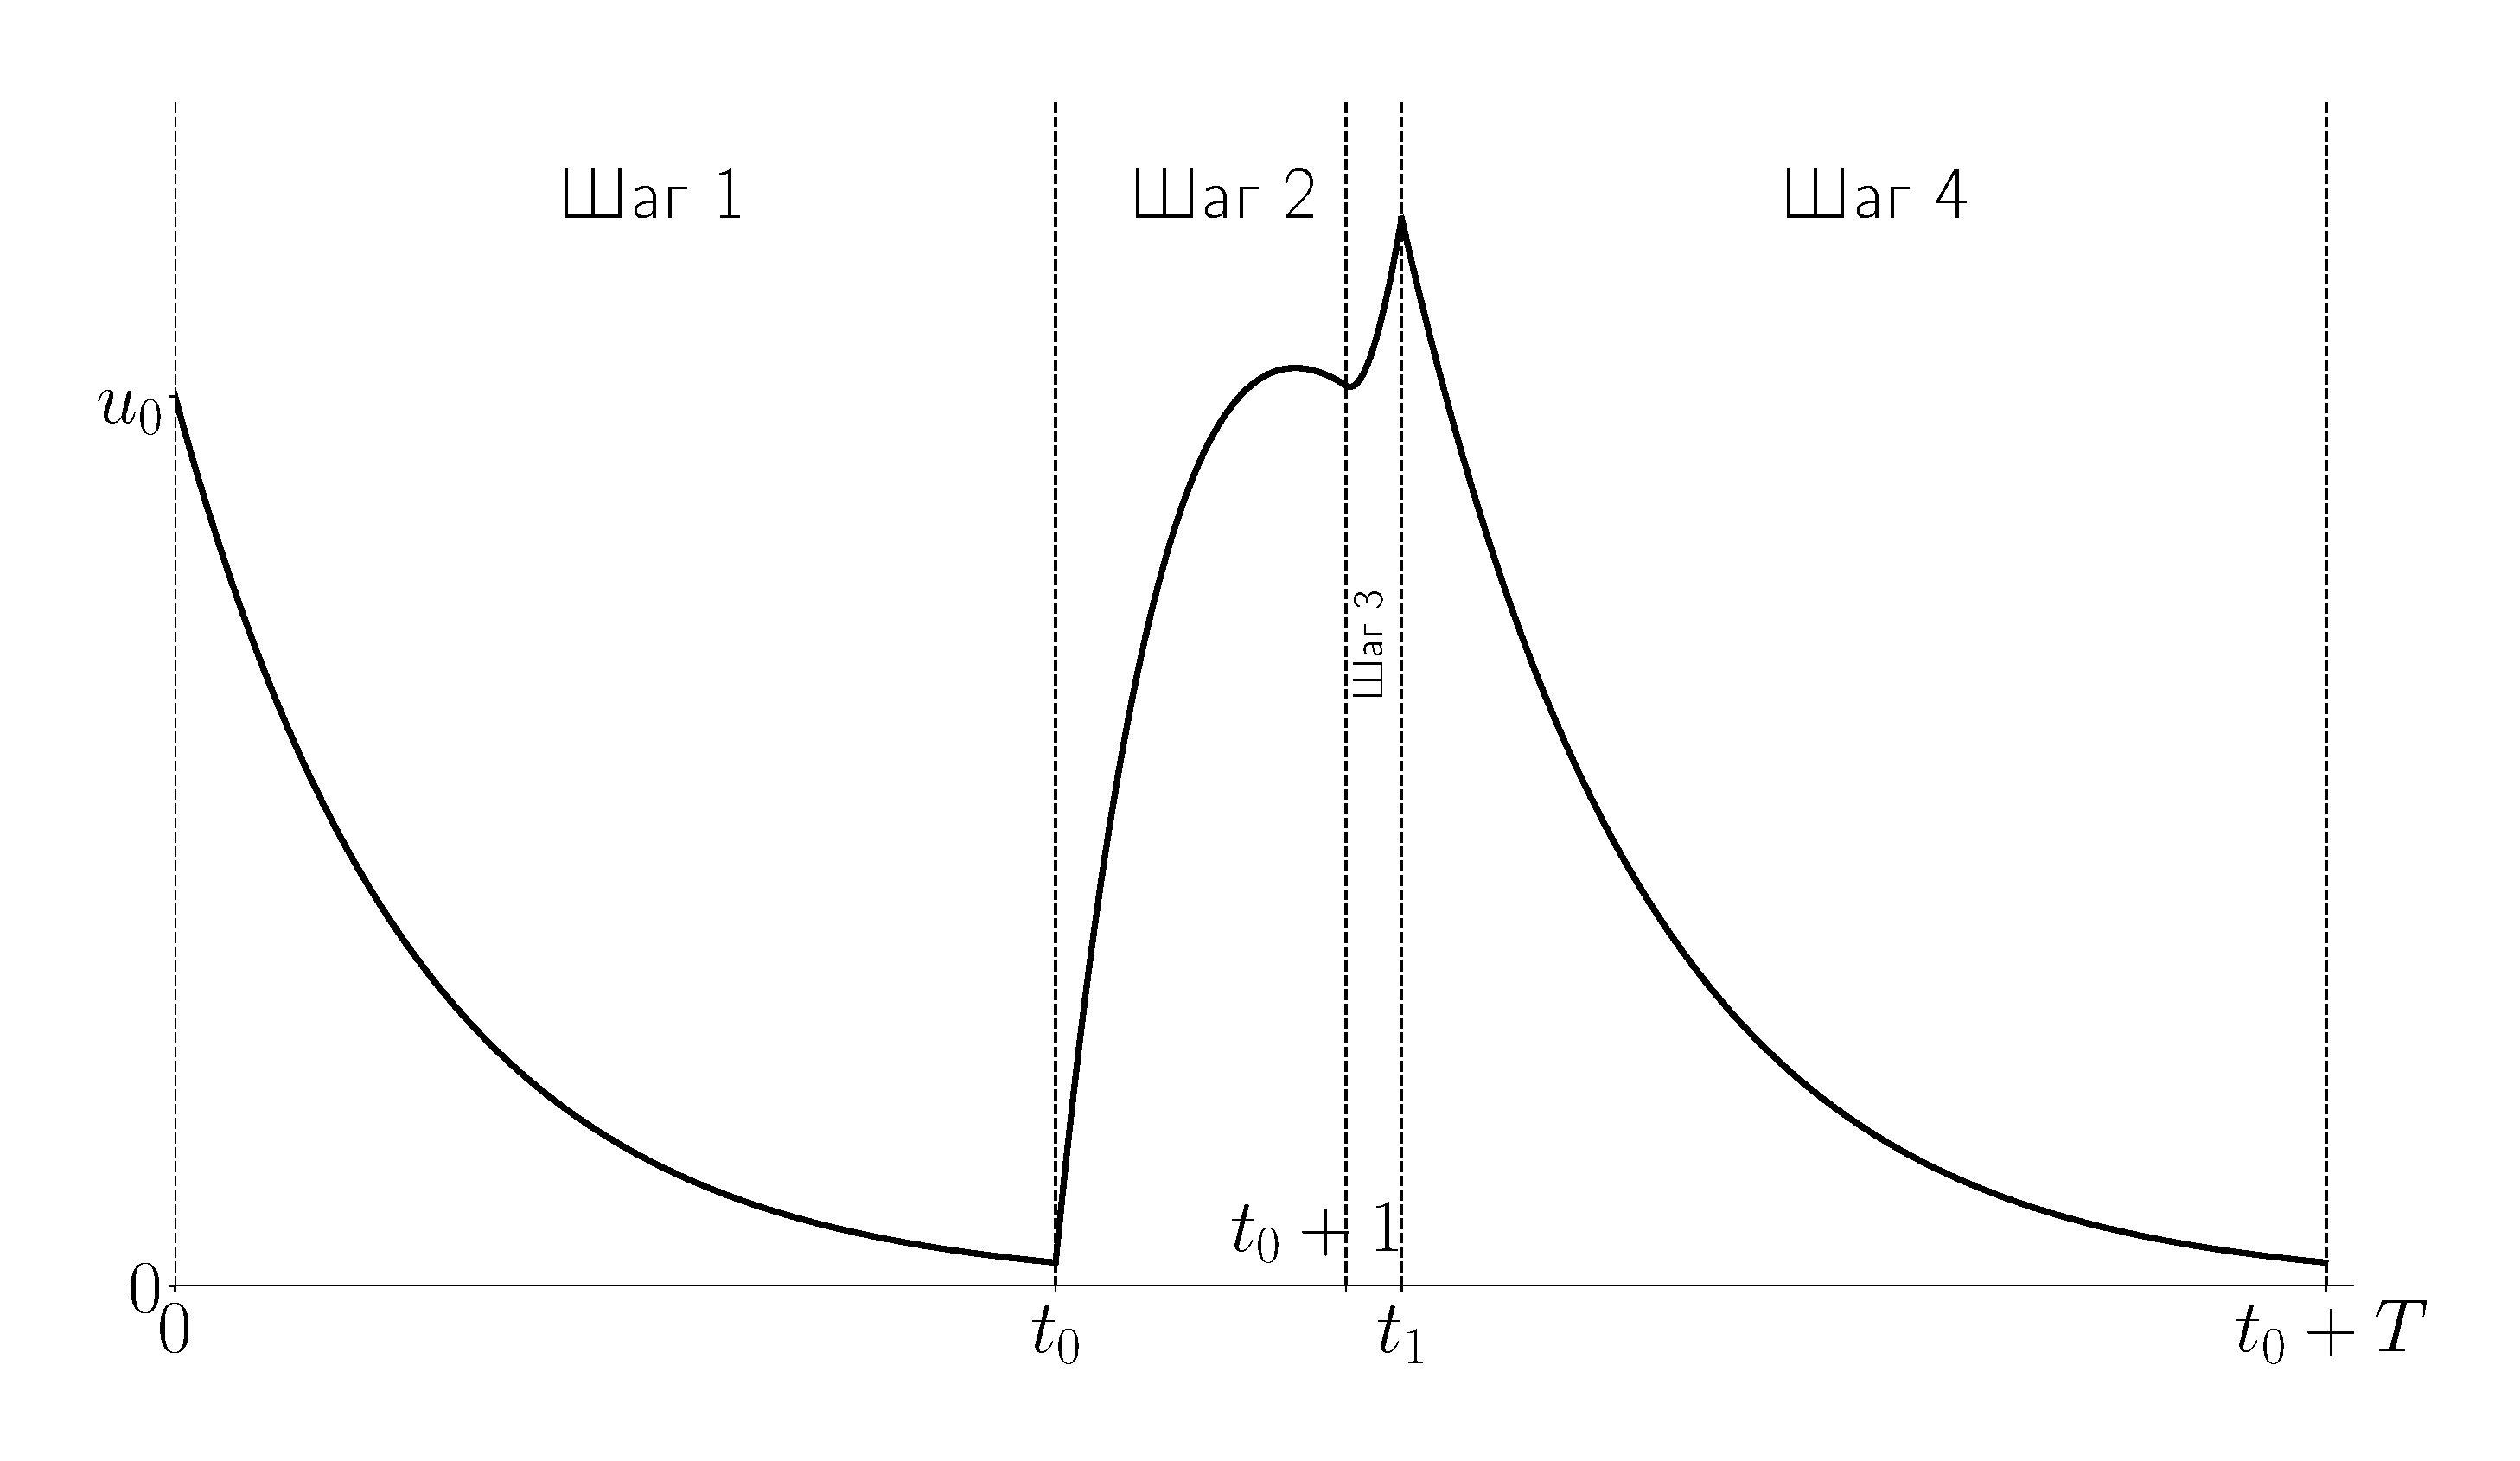
\includegraphics[width=0.7\textwidth]{u_star.eps}
	\caption{Функция $u_*(t)$, определённая на периоде $[t_0, t_0 + T]$ уравнением \eqref{eq:u_star}.}
\end{figure}

Докажем сформулированную теорему.


Будем искать решение уравнения \eqref{eq:mg_relay_w} методом шагов, последовательно рассматривая временные отрезки между точками переключения. 

\paragraph{Шаг 1.} 
Проследим за функцией $w(t)=u(t-1)+u(t-\tau_1)+\ldots+u(t-\tau_m)$ на отрезках $[0, 1]$, $[1, \tau_1]$, \dots, $[\tau_{m-1}$, $\tau_{m}]$. Величины $t - 1$, $t - \tau_1$, \dots, $t - \tau_m$ при $t \in [0,1]$ изменяются на отрезке $[-\tau_m,0]$, а значит, здесь 
%
\begin{equation*}
	w(t)=\varphi(t-1)+\varphi(t-\tau_1)+\ldots+\varphi(t-\tau_m) > m+1 > 1
\end{equation*}
%
и $F(w(t))=0$. Таким образом, 
$u(t)$ при $t\in[0,1]$ отыскивается из задачи Коши 
%
\begin{equation*}
	\dot{u}=-\beta u,\quad u(0)=u_0,
\end{equation*}
%
следовательно, описывается формулой 
%
\begin{equation*}
	u(t)=u_0e^{-\beta t}.
\end{equation*}
%
Эта формула сохранится по крайней мере на отрезке $[0,\tau_m]$, так как в $w(t)$ везде на этом промежутке входит слагаемое $\varphi(t - \tau_m) > 1$, и при переходе через точки $\tau_k$, $k = 1, \ldots, m$, слагаемое $\varphi(t-\tau_k)$ в $w(t)$ заменяется на $u_0e^{\beta (t-\tau_k)} > 0$, то есть свойство $w(t) > 1$ сохраняется. Какой бы ни была функция $\varphi\in S$, начиная с $\tau_m$, $w(t)$ имеет следующий вид, определяемый формулой $u(t)=u_0e^{-\beta t}$:
\begin{equation}
	\label{eq:w_step1}
	w(t)=u_0 e^{-\beta(t-1)} + u_0 e^{-\beta(t-\tau_1)} + \ldots + u_0 e^{-\beta(t-\tau_m)}=u_0 A e^{-\beta t}.
\end{equation} 

Формула $u(t)=u_0 e^{-\beta t}$ сохраняется до точки $t_0$, в которой $w(t)$ обращается в 1.

Таким образом, получаем, что 
\begin{equation}
	\label{eq:u_step1}
	u(t)=u_*(t)=u_0e^{-\beta t} \text{ при }t\in[0, t_0].
\end{equation}

Учитывая вид \eqref{eq:w_step1} функции $w(t)$, получаем \begin{equation}
	\label{eq:t0}
	t_0 = \frac{1}{\beta}\ln(u_0 A).
\end{equation}

Далее, начиная с точки $t_0$ в правой части уравнения \eqref{eq:mg_relay_w} величина $F(w(t))$ перестает быть нулем, поскольку аргумент становится меньше $1$. Для построения решения при $t > t_0$ докажем следующий факт.

\begin{lemma}
	\label{lm:u_star}
	На каждом шаге, пока $w(t) < 1$, функция $u(t)$ отыскивается из задачи Коши вида 
	\begin{equation}
		\label{eq:u_cauchy}
		\dot{u}=-\beta u + \alpha u_0 e^{-\beta t} P(t),\quad u(\tilde{t})=u_0 e^{-\beta \tilde{t}}\tilde{u},
	\end{equation}
	где константы $\tilde{t}$, $\tilde{u}$ и многочлен $P(t)$ определяются явно из предыдущего шага.
	Решение задачи \eqref{eq:u_cauchy} имеет вид
	\begin{equation}
		\label{eq:u_cauchy_sol}
		u(t) = u_0 e^{-\beta t}(\tilde{u}+\alpha \int_{\tilde{t}}^{t} P(s)\,ds) = u_0 e^{-\beta t} Q(t),
	\end{equation}
	где $Q(t)$ также является многочленом.
\end{lemma}

\begin{proof}
	Докажем лемму методом индукции. На первом шаге мы имеем $P(t) \equiv 0$, $\tilde{t} = 0$, $\tilde u = 1$. Выше было показано, что в это случае решение действительно имеет вид
	%
	\begin{equation*}
		u(t) = u_0 e^{-\beta t},
	\end{equation*}
	%
	здесь $Q(t) \equiv 1$. База индукции доказана.
	
	Теперь рассмотрим задачу \eqref{eq:u_cauchy} на некотором шаге построения решения. Будем искать решение в виде
	\begin{equation}
		\label{eq:lm_ustar_cauchy}
		u(t) = u_0 e^{-\beta t} Q(t).
	\end{equation}
	%
	Подставляя в \eqref{eq:u_cauchy}, получаем
	\begin{equation*}
		\frac{d}{dt}\left(u_0 e^{-\beta t} Q(t)\right) = -\beta e^{-\beta t} u_0 Q(t) + \alpha u_0 e^{-\beta t} P(t). 
	\end{equation*}
	\begin{equation*}
		u_0 e^{-\beta t} (-\beta Q(t) + \dot{Q}(t)) = -\beta u_0 e^{-\beta t} Q(t) + \alpha u_0 e^{-\beta t} P(t).
	\end{equation*}
	\begin{equation*}
		\dot{Q}(t) = \alpha P(t).
	\end{equation*}
	Это уравнение явно интегрируется:
	\begin{equation*}
		Q(t) - Q(\tilde{t}) = \alpha \int\limits_{\tilde{t}}^t P(s)\,ds.
	\end{equation*}
	Из начальных условий задачи \eqref{eq:u_cauchy} следует, что $Q(\tilde{t}) = \tilde{u}$, откуда получаем
	\begin{equation*}
		Q(t) = \tilde{u} + \int\limits_{\tilde{t}}^t P(s)\,ds.
	\end{equation*}
	Подставляя в \eqref{eq:lm_ustar_cauchy}, получаем требуемое:
	\begin{equation*}
		u(t) = u_0 e^{-\beta t} \left(\tilde{u} + \int\limits_{\tilde{t}}^t P(s)\,ds\right),
	\end{equation*}
	где множитель в скобках действительно является полиномом от $t$.
\end{proof}

\paragraph{Шаг 2.} Следующий промежуток построения --- это 
$[t_0, \min\{t_0 + 1, t_1\}]$.
Покажем, что $t_0+1 < t_1$, то есть точка переключения $t_1$ не может быть найдена на втором шаге и принадлежать отрезку $[t_0, t_0 + 1]$.
\begin{lemma}
	\label{lm:u_step2}
	$w(t)<1$ при $t \in (t_0, t_0 + 1]$.
\end{lemma}
\begin{proof}
	Рассмотрим функцию $w(t)$ на промежутке $t \in (t_0,t_0+1]$. Здесь величины $t - 1$, $t - \tau_1$, \dots, $t - \tau_m$ попадают в промежуток $(0, t_0]$, на котором $u(t)$ описывается формулой \eqref{eq:u_step1}. Это означает, что $w(t)$ описывается здесь формулой \eqref{eq:w_step1} и уравнение $w(t) = 1$ принимает вид $u_0 A e^{-\beta t} = 1$, как на первом шаге. Однако это  уравнение имеет единственный корень \eqref{eq:t0}, следовательно, $w(t) < 1$ при $t \in (t_0, t_0 + 1]$.
\end{proof}

Таким образом, следующий промежуток построения решения --- это $[t_0,t_0+1]$. Применим лемму \eqref{lm:u_star} при $P(t)\equiv A$, $\tilde{t} = t_0$, $\tilde{u} = 1$, получаем, что на отрезке $t \in [t_0, t_0 + 1]$ верно
\begin{equation}
	\label{eq:u_step2}
	u_*(t)= u_0 e^{-\beta t}\left(1 + \alpha\int\limits_{t_0}^t A\,ds \right) = u_0 e^{-\beta t}(\alpha A(t-t_0) + 1).
\end{equation}

\paragraph{Шаг 3.} Очередной промежуток построения --- это $[t_0 + 1, \min\{t_0 + \tau_*, t_1\}]$. На этом промежутке
На этом промежутке
\begin{multline}
	\label{eq:w3}
	w(t)=u_0 e^{-\beta (t-1)}(\alpha A(t-t_0-1)+1)+u_0 e^{-\beta(t - \tau_1)} + \ldots + u_0 e^{-\beta(t-\tau_m)} = \\
	= u_0 A e^{-\beta t}(1 + \alpha e^{\beta}(t - t_0 - 1)).
\end{multline}
Поскольку мы рассматриваем случай минимального числа точек переключения на периоде, будем считать, что $\tau_* \in (t_0 + 1, t_1)$. Условия, при которых это верно, будут сформулированы и доказаны далее.

Таким образом, следующий промежуток построения $[t_0 + 1, t_1]$. Учитывая формулу \eqref{eq:w3} и применяя лемму \ref{lm:u_star} при $P(t) = A(1 + \alpha e^\beta(t - t_0 - 1))$, $\tilde{t} = t_0+1$, $\tilde{u}=\alpha A+1$, получаем
\begin{multline}
	\label{eq:u_step3}
	u_*(t) = u_0 e^{-\beta t}\left(1 + \alpha\int\limits_{t_0 + 1}^t A(1 + \alpha A + \alpha e^\beta(s - t_0 - 1)) \,ds \right) =\\= u_0 e^{-\beta t}\left(\dfrac{\alpha^2}{2}Ae^{\beta}(t-t_0-1)^2+\alpha A(t-t_0)+1\right)\text{ при }t\in[t_0+1,t_1].
\end{multline}

\paragraph{Шаг 4.} Следующий промежуток построения функции $u(t)$ --- это $(t_1, t_2]$, на котором $w(t) > 1$. Здесь $F(w(t)) = 0$. Пусть для краткости $u_1 = u_*(t_1)$. Учитывая формулу \eqref{eq:u_step3},
\begin{equation*}
	u_1 = u(t_1) = u_0 e^{-\beta t_1}\left(\dfrac{\alpha^2}{2}Ae^{\beta}(t_1 - t_0 - 1)^2+\alpha A(t_1 - t_0)+1\right).
\end{equation*}
Тогда решение на этом промежутке находится из задачи Коши
\begin{equation*}
	\dot{u}=-\beta u,\quad u(t_1)=u_1.
\end{equation*}
Отсюда 
\begin{multline}
	\label{eq:u_step4}
	u_*(t)= u_1 e^{-\beta(t - t_1)} =\\= u_0 e^{-\beta t}\left(\dfrac{\alpha^2}{2}Ae^{\beta}(t_1 - t_0 - 1)^2 + \alpha A(t_1 - t_0) + 1\right) \text{ при } t \in (t_1,t_2].
\end{multline}
%
\subsection{Область параметров, при которых $t_1\in (t_0+1,t_0+\tau_*)$.}

Покажем, что из условий \eqref{eq:cond_thm1}, \eqref{eq:cond_thm2} теоремы \ref{th:mg_auxiliary_main} следует, что $t_1 \in (t_0+1,t_0+\tau_*)$.

В уравнении \eqref{eq:w3} сделаем замену $s = t - t_0$. С учётом $u_0A=e^{\beta t_0}$, получаем, что уравнение $w(t)=1$ принимает на рассматриваемом промежутке следующую форму:
\begin{equation}
	\label{eq:f}
	e^{\beta s} - \alpha e^{\beta}(s-1) - 1 = 0.
\end{equation}

Обозначим левую часть уравнения как $f(s)$. Поскольку $f''(s) = \beta^2 e^{\beta s} > 0$, функция $f(s)$ выпукла.

\begin{lemma}
	\label{lm:t1_existence}
	Существование корня $s_* > 1$ уравнения \eqref{eq:f} равносильно условию \eqref{eq:cond_thm1}.
\end{lemma}
\begin{proof}
	$f(1) = e^{\beta} - 1 > 0$. Тогда существование корня эквивалентно условию
	%
	\begin{equation*}
		\min\limits_{s > 1}f(s) < 0.
	\end{equation*}
	
	Найдём точку минимума $s_{\min}$ функции $f(s)$.
	\begin{equation*}
		f'(s) = 0 \ \Leftrightarrow \ \beta e^{\beta s} - \alpha e^{\beta} = 0\ \Leftrightarrow\ s = 1 + \frac{1}{\beta}\ln\frac{\alpha}{\beta}.
	\end{equation*}
	Поскольку $f(s)$ выпукла, это действительно точка минимума. Подставим её в условие $f(s_{\min}) < 0$:
	\begin{equation*}
		\exp\left(\beta (1 + \frac{1}{\beta}\ln\frac{\alpha}{\beta}) \right) - \alpha e^{\beta}(1 + \frac{1}{\beta}\ln\frac{\alpha}{\beta} - 1) - 1 < 0 \Leftrightarrow
	\end{equation*}
	\begin{equation*}
		\frac{\alpha}{\beta}e^{\beta}\left(1 + \ln\frac{\beta}{\alpha}\right) < 1,
	\end{equation*}
	что соответствует первой части условия \eqref{eq:cond_thm1}.
	
	Если $s_{\min} < 1$, то корень уравнения \eqref{eq:f} также будет меньше $1$ (в случае существования). Поэтому условию $s_* > 1$ соответствует ограничение $s_{\min} > 1$:
	\begin{equation*}
		1 + \frac{1}{\beta}\ln\frac{\alpha}{\beta} > 1 \quad \Leftrightarrow \quad \alpha > \beta.
	\end{equation*}
\end{proof}

\begin{lemma}
	\label{lm:t1_locate}
	Пусть выполнены условия леммы \ref{lm:t1_existence}. Корень $s_*$ уравнения \eqref{eq:f} (меньший, если их два) принадлежит промежутку $(1,\tau_*]$ тогда и только тогда, когда выполняется хотя бы одно из двух условий:
	\begin{enumerate}
		\item[1)] $e^{\beta \tau_*} - 1 \leqslant \alpha e^\beta(\tau_* - 1)$,
		\item[2)] $0 < \frac{1}{\beta}\ln\frac{\alpha}{\beta}\leqslant\tau_*-1$.
	\end{enumerate}
\end{lemma}
\begin{proof}
	Поскольку $f(1) > 0$, возможны две ситуации: $f(\tau_*) \leqslant 0$ или $f(\tau_*) > 0$, но $s_{\min} \leq \tau_*$, см. рисунок \ref{fig:tau_star}.

\begin{figure}[ht]
	\centering
	\begin{minipage}{.45\linewidth}
		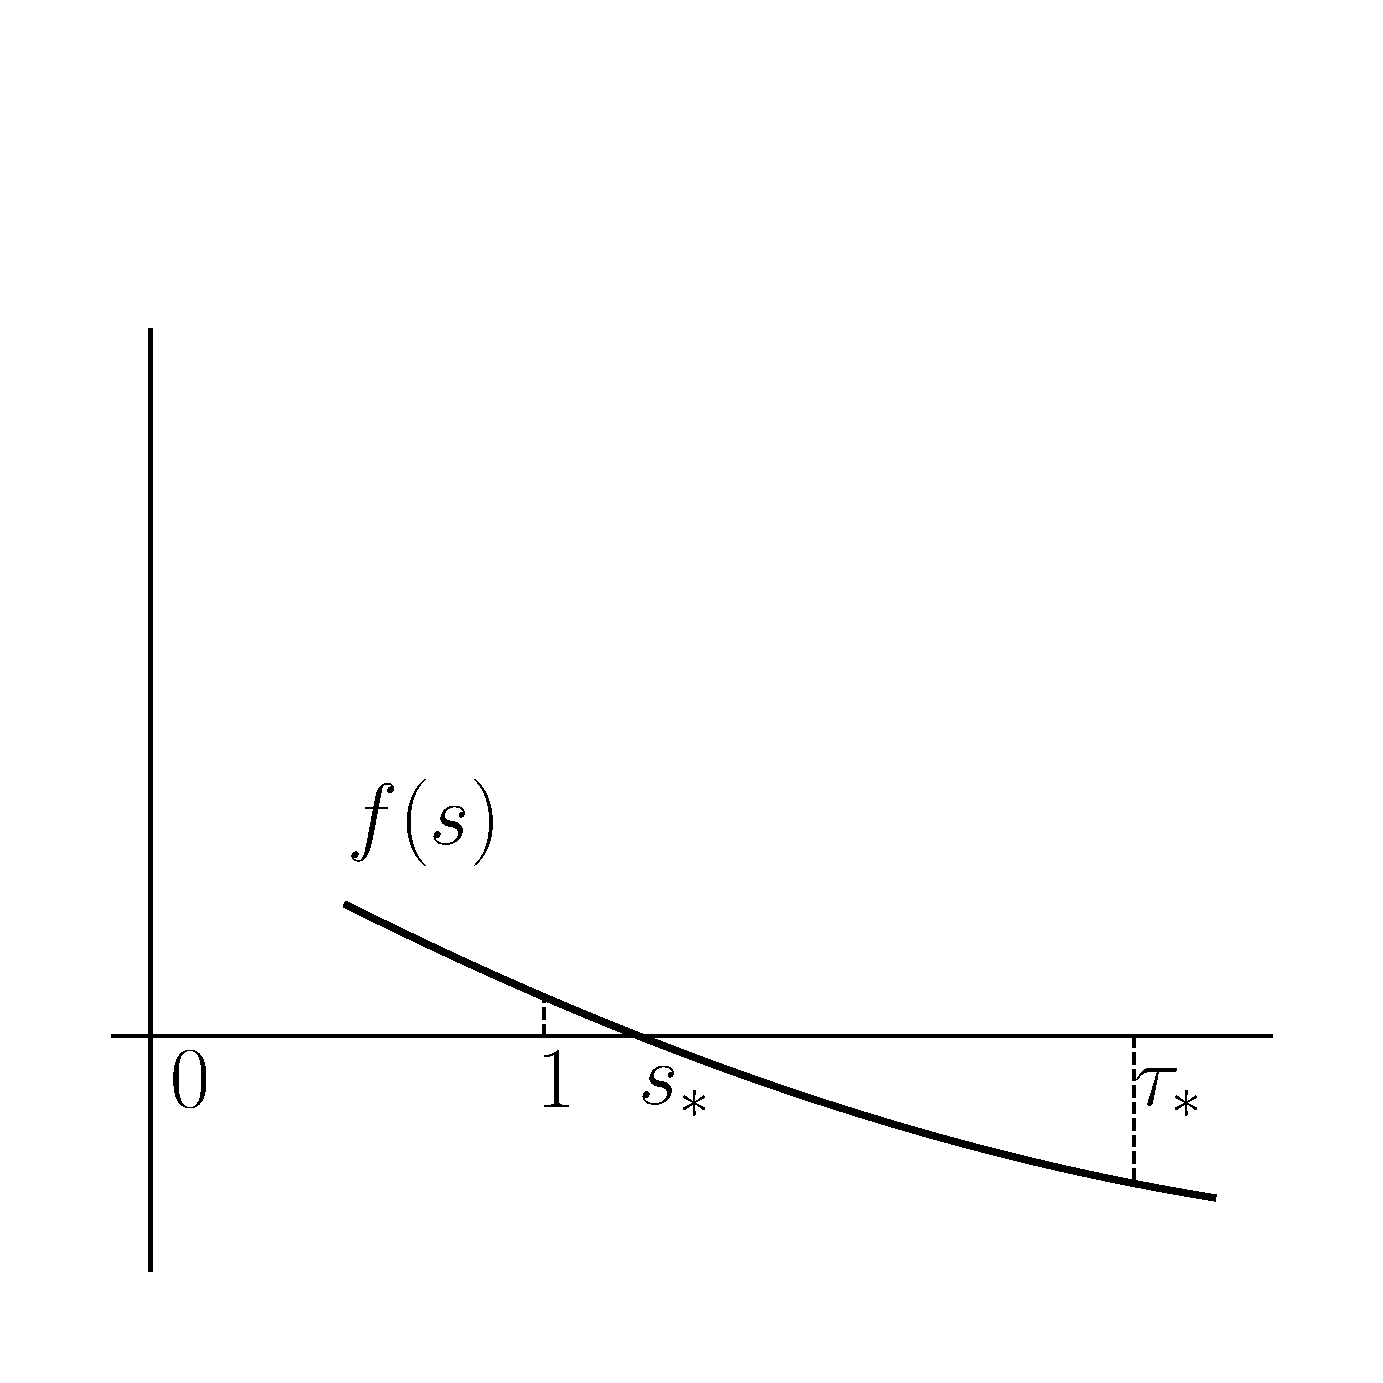
\includegraphics[width=\linewidth]{images/f2.eps}
	\end{minipage}
	\hspace{.05\linewidth}
	\begin{minipage}{.45\linewidth}
		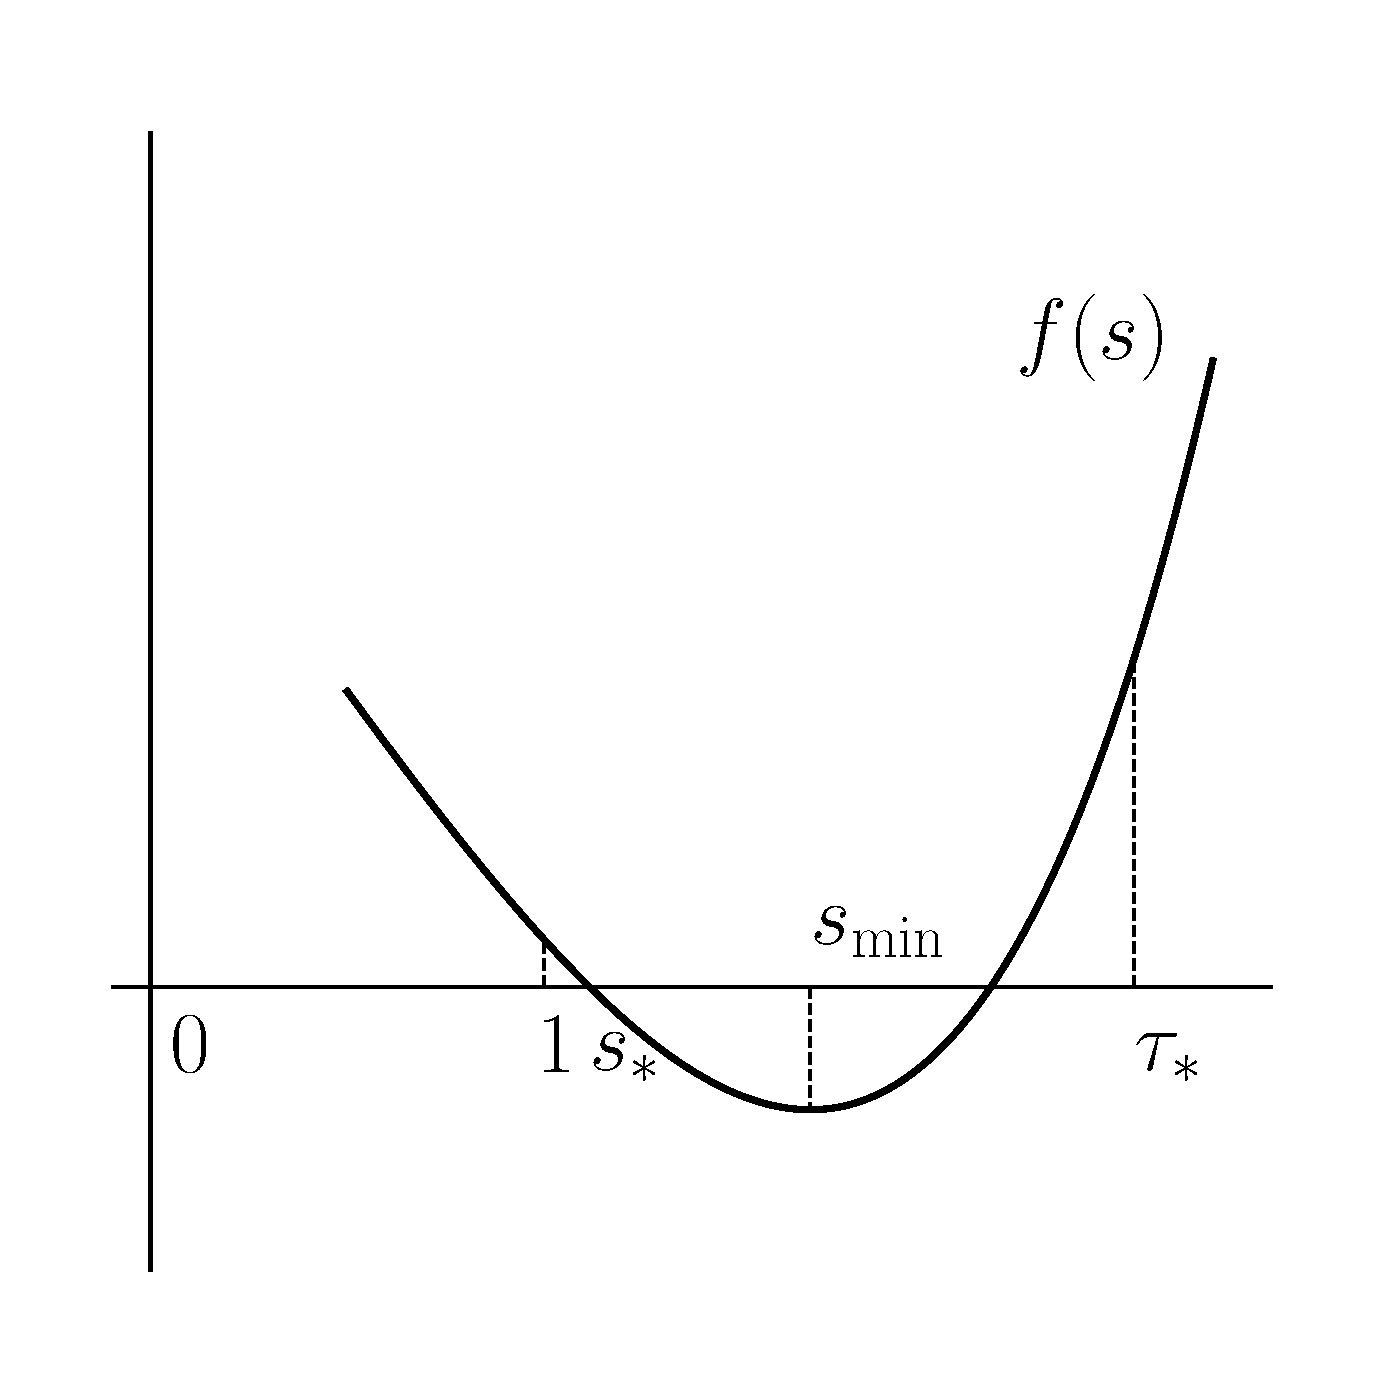
\includegraphics[width=\linewidth]{images/f1.eps}
	\end{minipage}
	\caption{Варианты взаимного расположения графика функции $f(s)$ при условии, что корень $s_*$ уравнения \eqref{eq:f} существует и попадает на интервал $(1,\tau_*)$. На левом изображении $f(1) > 0$ и $f(\tau_*) \leq 0$. На правом рисунке $f(1) > 0$ и $f(\tau_*) > 0$, но точка минимума $s_{\min}$ принадлежит промежутку $(1,\tau_*]$.}
	\label{fig:tau_star}
\end{figure}

Случай $f(\tau_*) \leq 0$ соответствует условию 1), случай $1 < s_{\min} \leqslant \tau_*$ --- условию 2) леммы. 
\end{proof}

Таким образом, мы доказали, что из условий \eqref{eq:cond_thm1} и \eqref{eq:cond_thm2} теоремы \ref{th:mg_auxiliary_main} следует, что корень $s_*$ уравнения \eqref{eq:f} существует и лежит между $1$ и $\tau_*$. Это означает, что точка переключения $t_1 = t_0 + s_*$ также существует и попадает на отрезок $[t_0 + 1, t_0 + \tau_*]$.

Далее мы опишем область значений параметров, удовлетворяющих условиям \eqref{eq:cond_thm1} и \eqref{eq:cond_thm2} явно.

\subsection{Явное описание области допустимых значений $\alpha$, $\beta$, $\tau_*$}

Выразим $\alpha$ из условия \eqref{eq:cond_thm1}.
\begin{equation*}
\frac{\alpha}{\beta}e^{\beta}\left(\ln\frac{\beta}{\alpha} + 1\right) \leqslant 1\ \Leftrightarrow\ 1 + \ln\dfrac{\beta}{\alpha} \leqslant \dfrac{\beta e^{-\beta}}{\alpha}.
\end{equation*}

Возьмём экспоненту от обеих частей:
\begin{equation*}
\dfrac{e\beta}{\alpha} \leqslant \exp\dfrac{\beta e^{-\beta}}{\alpha}\ \Leftrightarrow\ \dfrac{-\beta e^{-\beta}}{\alpha}\exp \dfrac{-\beta e^{-\beta}}{\alpha} \geqslant -e^{-\beta - 1}\ \Leftrightarrow
\end{equation*}

\begin{align}
\label{eq:step3_cond1_expanded}
\left[
\begin{array}{ll}
	-\frac{\beta e^{-\beta}}{\alpha} \geqslant W_0(-e^{-\beta - 1}),\\
	-\frac{\beta e^{-\beta}}{\alpha} \leqslant W_{-1}(-e^{-\beta - 1}).
\end{array}
\right.
\end{align}
%
где $W_0(x)$ --- ветвь W-функции Ламберта, определённая при $x \in [-1; +\infty)$, а $W_{-1}(x)$ --- ветвь, определённая при $x \in (-\infty; -1]$.

Однако, второе неравенство соответствует случаю $\dfrac{-\beta e^{-\beta}}{\alpha} < -1$ (поскольку $W_{-1}(x)$ определена при $x < -1$). Тогда
\begin{equation*}
\alpha < \beta e^{-\beta} < \beta,
\end{equation*}
что противоречит условию \eqref{eq:cond_thm1}.

Значит, в совокупности неравенств \eqref{eq:step3_cond1_expanded} заменяется на единственное неравенство
\begin{equation}
\label{eq:step3_cond1}
-\frac{\beta e^{-\beta}}{\alpha} \geqslant W(-e^{-\beta - 1})
\end{equation}
Здесь и далее, будем писать $W$ вместо $W_0$ для обозначения соответствующей функции Ламберта.

Определим функцию
\begin{equation}
\label{eq:step_3_phi_func}
\varphi(\beta) = - \dfrac{\beta e^{-\beta}}{W_0(-e^{-\beta - 1})}.
\end{equation}
%
В этих обозначениях условие \eqref{eq:step3_cond1} перепишется как
%
\begin{equation}
\label{eq:step_3_cond_phi}
\alpha \geqslant \varphi(\beta).
\end{equation}

Теперь выразим $\alpha$ из условия \eqref{eq:cond_thm2}:
\begin{equation}
\label{eq:step3_cond2_expanded_1}
e^{\beta \tau_*}-1\leqslant\alpha e^\beta(\tau_*-1)\ \Leftrightarrow\ \alpha \geqslant \dfrac{e^{\beta \tau_*}-1}{e^\beta(\tau_*-1)}.
\end{equation}
\begin{equation}
\label{eq:step3_cond2_expanded_2}
\frac{1}{\beta}\ln\frac{\alpha}{\beta}\leqslant\tau_*-1\ \Leftrightarrow\ \alpha \leqslant \beta e^{\beta (\tau_* - 1)}.
\end{equation}

Определим функции
\begin{equation}
\label{eq:step_3_theta_func}
\theta(\beta, \tau_*) = \dfrac{e^{\beta \tau_*}-1}{e^\beta(\tau_*-1)}.
\end{equation}
%
\begin{equation}
\label{eq:step_3_psi_func}
\delta(\beta, \tau_*) = \beta e^{\beta (\tau_* - 1)}.
\end{equation}
%
В этих обозначениях условие \eqref{eq:cond_thm2} перепишется как
%
\begin{equation}
\label{eq:step_3_cond_2}
\left[
\begin{array}{ll}
	\alpha \geqslant \theta(\beta, \tau_*),\\
	\alpha \leqslant \delta(\beta, \tau_*).
\end{array}
\right.
\end{equation}

Исследуем взаимное расположение функций $\phi$, $\theta$ и $\delta$.

\begin{lemma}
\label{lm:tau_star_sol}
Уравнение 
\begin{equation}
	e^{\beta x}(\beta(x - 1) - 1) + 1 = 0.
\end{equation}
при фиксированном $\beta > 0$ имеет единственный корень, больший единицы:
\begin{equation}
	x = 1 + \frac{1 + W(-e^{-\beta - 1})}{\beta}.
\end{equation}
\end{lemma}
\begin{proof}

\begin{multline*}
	e^{\beta x}(\beta(x - 1) - 1) = -1 \Leftrightarrow e^{\beta(x - 1) - 1}(\beta(x - 1) - 1) = -e^{-\beta - 1}\ \Leftrightarrow\\\Leftrightarrow\ \beta(x - 1) - 1 = W(-e^{-\beta - 1})\ \Leftrightarrow\ x = 1 + \dfrac{1 + W(-e^{-\beta - 1})}{\beta}.
\end{multline*}

Здесь применение функции $W$ корректно, поскольку $\beta(x - 1) - 1 > -1$ и $-e^{-\beta - 1} > -\frac{1}{e}$.

\end{proof}


\begin{lemma}
	\label{lm:beta_tilde_sol}
	Уравнение 
	\begin{equation*}
		e^{\beta x}(\beta(x - 1) - 1) + 1 = 0.
	\end{equation*}
	при фиксированном $x > 1$ имеет единственный положительный корень:
	\begin{equation*}
		\tilde{\beta}(x) = \frac{1}{x - 1} + \frac{1}{x}W\left(\frac{x}{1 - x} e^{\frac{x}{1 - x}}\right).
	\end{equation*}
\end{lemma}

\begin{proof}
	Перенесём единицу в правую часть:
	%
	\begin{equation*}
		e^{\beta x}(\beta(x - 1) - 1) = -1.
	\end{equation*}
	%
	Домножим на $\frac{x}{x - 1}$:
	%
	\begin{equation*}
		e^{\beta x}\left( \beta x + \frac{x}{x - 1} \right) = -\frac{x}{x - 1}. 
	\end{equation*}
	%
	Домножим обе части уравнения на $e^{\frac{x}{x - 1}}$:
	%
	\begin{equation*}
		\left( \beta x - \frac{x}{1 - x} \right) e^{\beta x - \frac{x}{1 - x}} = \frac{x}{1 - x} e^{\frac{x}{1 - x}}. 
	\end{equation*}
	%
	Функция $f(t) = t e^t$ принимает значение $\frac{x}{1 - x} e^{\frac{x}{1 - x}}$ ровно в двух точках: $t = \frac{x}{1 - x} < -1$ и $t = W\left(\frac{x}{1 - x} e^{\frac{x}{1 - x}}\right) \in (-1; 0)$.
	
	\begin{align*}
		\left[
		\begin{array}{ll}
			\beta x + \frac{x}{1 - x} = \frac{x}{1 - x};\\
			\beta x + \frac{x}{1 - x} = W\left(\frac{x}{1 - x} e^{\frac{x}{1 - x}}\right).
		\end{array}
		\right.
	\end{align*}
	
	Первое равенство при допустимых значениях параметров не имеет решений, второе даёт единственное решение
	\[
	\beta = \frac{1}{x - 1} + \frac{1}{x} W\left(\frac{x}{1 - x} e^{\frac{x}{1 - x}}\right).
	\]
\end{proof}

\begin{proposition}
	\label{prop:phi_theta}
	$\phi(\beta) = \min\limits_{\tau_* > 1} \theta(\beta, \tau_*)$.
\end{proposition}

\begin{proof}
	\begin{equation*}
		\frac{d}{d\tau_*} \theta(\beta, \tau_*) = \frac{d}{d\tau_*} \left( \frac{e^{\beta\tau_*} - 1}{e^{\beta}(\tau_* - 1)} \right) = \frac{e^{-\beta}\left(e^{\beta \tau_*}(\beta(\tau_* - 1) - 1) + 1\right)}{(\tau_* - 1)^2}.
	\end{equation*}
	Нуль производной соответствует решению уравнения
	\begin{equation*}
		e^{\beta \tau_*}(\beta(\tau_* - 1) - 1) + 1 = 0
	\end{equation*}
	относительно $\tau_*$. По лемме \ref{lm:tau_star_sol}, такое решение существует и единственно при $\tau_* > 1$, обозначим его
	\begin{equation*}
		\tau_*^{\min} = 1 + \frac{1 + W(-e^{-\beta - 1})}{\beta}.
	\end{equation*}
	Заметим, что оно действительно будет точкой минимума функции $ \theta(\beta, \tau_*)$ при фиксированном $\beta$, поскольку
	\begin{equation*}
		\lim\limits_{\tau_* \to 1 + 0} \theta(\beta, \tau_*) = \lim\limits_{\tau_* \to +\infty} \theta(\beta, \tau_*) = +\infty. 
	\end{equation*}
	
	Из условия
	\begin{equation*}
		e^{\beta \tau_*^{\min}}(\beta(\tau_*^{\min} - 1) - 1) + 1 = 0
	\end{equation*}
	выразим $e^{\beta \tau_*^{\min}} - 1$:
	\begin{equation*}
		e^{\beta \tau_*^{\min}} - 1 = \beta e^{\beta \tau_*^{\min}} (\tau_*^{\min} - 1)
	\end{equation*}
	и подставим в функцию $\theta(\beta, \tau_*)$:
	\begin{multline}
		\theta(\beta, \tau_*^{\min}) = \frac{e^{\beta\tau_*^{\min}} - 1}{e^{\beta}(\tau_*^{\min} - 1)} = \frac{\beta e^{\beta \tau_*^{\min}} (\tau_*^{\min} - 1)}{e^{\beta}(\tau_*^{\min} - 1)} =\\= \beta e^{\beta (\tau_*^{\min} - 1)} = \beta e^{\beta(1 + \frac{1 + W(-e^{-\beta - 1})}{\beta} - 1)} = \beta e^{1 + W(-e^{-\beta - 1})}. 
	\end{multline}
	
	Теперь убедимся, что $\theta(\beta, \tau_*^{\min}) = \phi(\beta)$.
	%
	\begin{equation*}
		\beta e^{1 + W(-e^{-\beta - 1})} = -\frac{\beta e^{-\beta}}{W(-e^{-\beta - 1})} \Leftrightarrow -e^{-\beta - 1} = W(-e^{-\beta - 1}) e^{W(-e^{-\beta - 1})},
	\end{equation*}
	что является верным равенством, поскольку $-e^{-\beta - 1} > -\frac{1}{e}$.
\end{proof}


\begin{proposition}
	\label{prop:delta_theta}
	$\delta(\beta, \tau_*) \geq \theta(\beta, \tau_*) \Leftrightarrow \beta \geq \tilde{\beta}(\tau_*)$ при $\beta > 0$, $\tau_* > 1$.  
\end{proposition}

\begin{proof}
	Решим относительно $\beta$ уравнение 
	\[
	\delta(\beta, \tau_*) = \theta(\beta, \tau_*).
	\]
	\[
	\beta e^{\beta(\tau_*- 1)} = \dfrac{e^{\beta \tau_*} - 1}{e^{\beta} (\tau_* - 1)} \Leftrightarrow e^{\beta\tau_*}(\beta(\tau_* - 1) - 1) = -1.
	\]
	По лемме \ref{lm:beta_tilde_sol}, единственное решение этого уравнения $\beta = \tilde{\beta}(\tau_*)$.
	
	При $\beta \to +\infty$ функция $\theta(\beta, \tau_*) \sim \frac{1}{\tau_* - 1}e^{\beta(\tau_* - 1)}$ асимптотически меньше, чем $\delta(\beta, \tau_*) = \beta e^{\beta (\tau_* - 1)}$. Из непрерывности следует, что при $\beta > \tilde{\beta}(\tau_*)$ верно неравенство
	\[
	\delta(\beta, \tau_*) > \theta(\beta, \tau_*).
	\]
	
	Теперь сравним функции при малых значениях $\beta > 0$. Заметим, что $\theta(0, \tau_*) = \delta(0, \tau_*) = 0$.
	\[
	\frac{d}{d\beta}\theta(\beta, \tau_*)\Bigg\vert_{\beta = 0} = e^{-\beta}\left( e^{\beta \tau_*} + \frac{1}{\tau_* - 1}\right)\Bigg\vert_{\beta = 0} = 1 + \frac{1}{\tau_* - 1} > 1;
	\]
	\[
	\frac{d}{d\beta}\delta(\beta, \tau_*)\Bigg\vert_{\beta = 0} = e^{\beta(\tau_* - 1)}(\beta(\tau_* - 1) + 1)\Bigg\vert_{\beta = 0} = 1.
	\]
	Поскольку
	\[
	\frac{d}{d\beta}\delta(\beta, \tau_*)\bigg\vert_{\beta = 0} < \frac{d}{d\beta}\theta(\beta, \tau_*)\bigg\vert_{\beta = 0},
	\]
	при малых значениях $\beta > 0$ выполнено неравенство
	\[
	\delta(\beta, \tau_*) < \theta(\beta, \tau_*),
	\]
	а из непрерывности оно распространяется на весь промежуток $\left(0, \tilde{\beta}(\tau_*)\right)$.    
\end{proof}


\begin{proposition}
	\label{prop:delta_phi}
	$\delta(\beta, \tau_*) \geq \phi(\beta) \Leftrightarrow \beta \geq \tilde{\beta}(\tau_*)$ при $\beta > 0$, $\tau_* > 1$.  
\end{proposition}

\begin{proof}
	Решим относительно $\beta$ неравенство 
	\[
	\delta(\beta, \tau_*) = \phi(\beta).
	\]
	\[
	-\dfrac{\beta e^{-\beta}}{W(-e^{-\beta - 1})} \geqslant \beta e^{\beta(\tau_* - 1)}\ \Leftrightarrow\ W(-e^{-\beta - 1}) \geqslant -e^{-\beta\tau_*}
	\]
	%
	Поскольку $-e^{-\beta - 1} \geqslant -e^{-1}$ и $-e^{-\beta\tau_*} \geqslant -1$, преобразование $x \mapsto x e^x$ является монотонным и взаимно однозначным.
	%
	\begin{multline*}
		-e^{-\beta - 1} \geqslant -e^{-\beta\tau_*}\exp(-e^{-\beta\tau_*})\ \Leftrightarrow\ e^{-\beta - 1 + \beta\tau_*} \leqslant \exp(-e^{-\beta\tau_*})\ \Leftrightarrow
		\\
		\Leftrightarrow\ -\beta - 1 + \beta\tau_* \leqslant -e^{-\beta \tau_*}\ \Leftrightarrow \ e^{\beta \tau_*}(\beta(\tau_* - 1) - 1) \leqslant -1\ \Leftrightarrow
		\\
		\Leftrightarrow\ \left(\beta \tau_* + \frac{\tau_*}{1 - \tau_*}\right) e^{\beta \tau_* + \frac{\tau_*}{1 - \tau_*}} \leqslant \frac{\tau_*}{1 - \tau_*} e^{\frac{\tau_*}{1 - \tau_*}}.
	\end{multline*}
	%
	Функция $f(x) = x e^x$ принимает значение $\frac{\tau_*}{1 - \tau_*} e^{\frac{\tau_*}{1 - \tau_*}}$ ровно в двух точках: $x = \frac{\tau_*}{1 - \tau_*} < -1$ и $x = W\left(\frac{\tau_*}{1 - \tau_*} e^{\frac{\tau_*}{1 - \tau_*}}\right) \in (-1; 0)$.
	
	Тогда равносильным будет переход к следующему неравенству (см. рис. \ref{fig:w_inverse}):
	\begin{equation}
		\label{eq:phi_double_inequality}
		\frac{\tau_*}{1 - \tau_*} \leqslant \beta \tau_* + \frac{\tau_*}{1 - \tau_*} \leqslant  W\left(\frac{\tau_*}{1 - \tau_*} e^{\frac{\tau_*}{1 - \tau_*}}\right).
	\end{equation}
	%
	Левая часть эквивалентна $\beta \geqslant 0$, а правая $\beta \leqslant \tilde{\beta}(\tau_*)$.
	%
	\begin{figure}[ht]
		\centering
		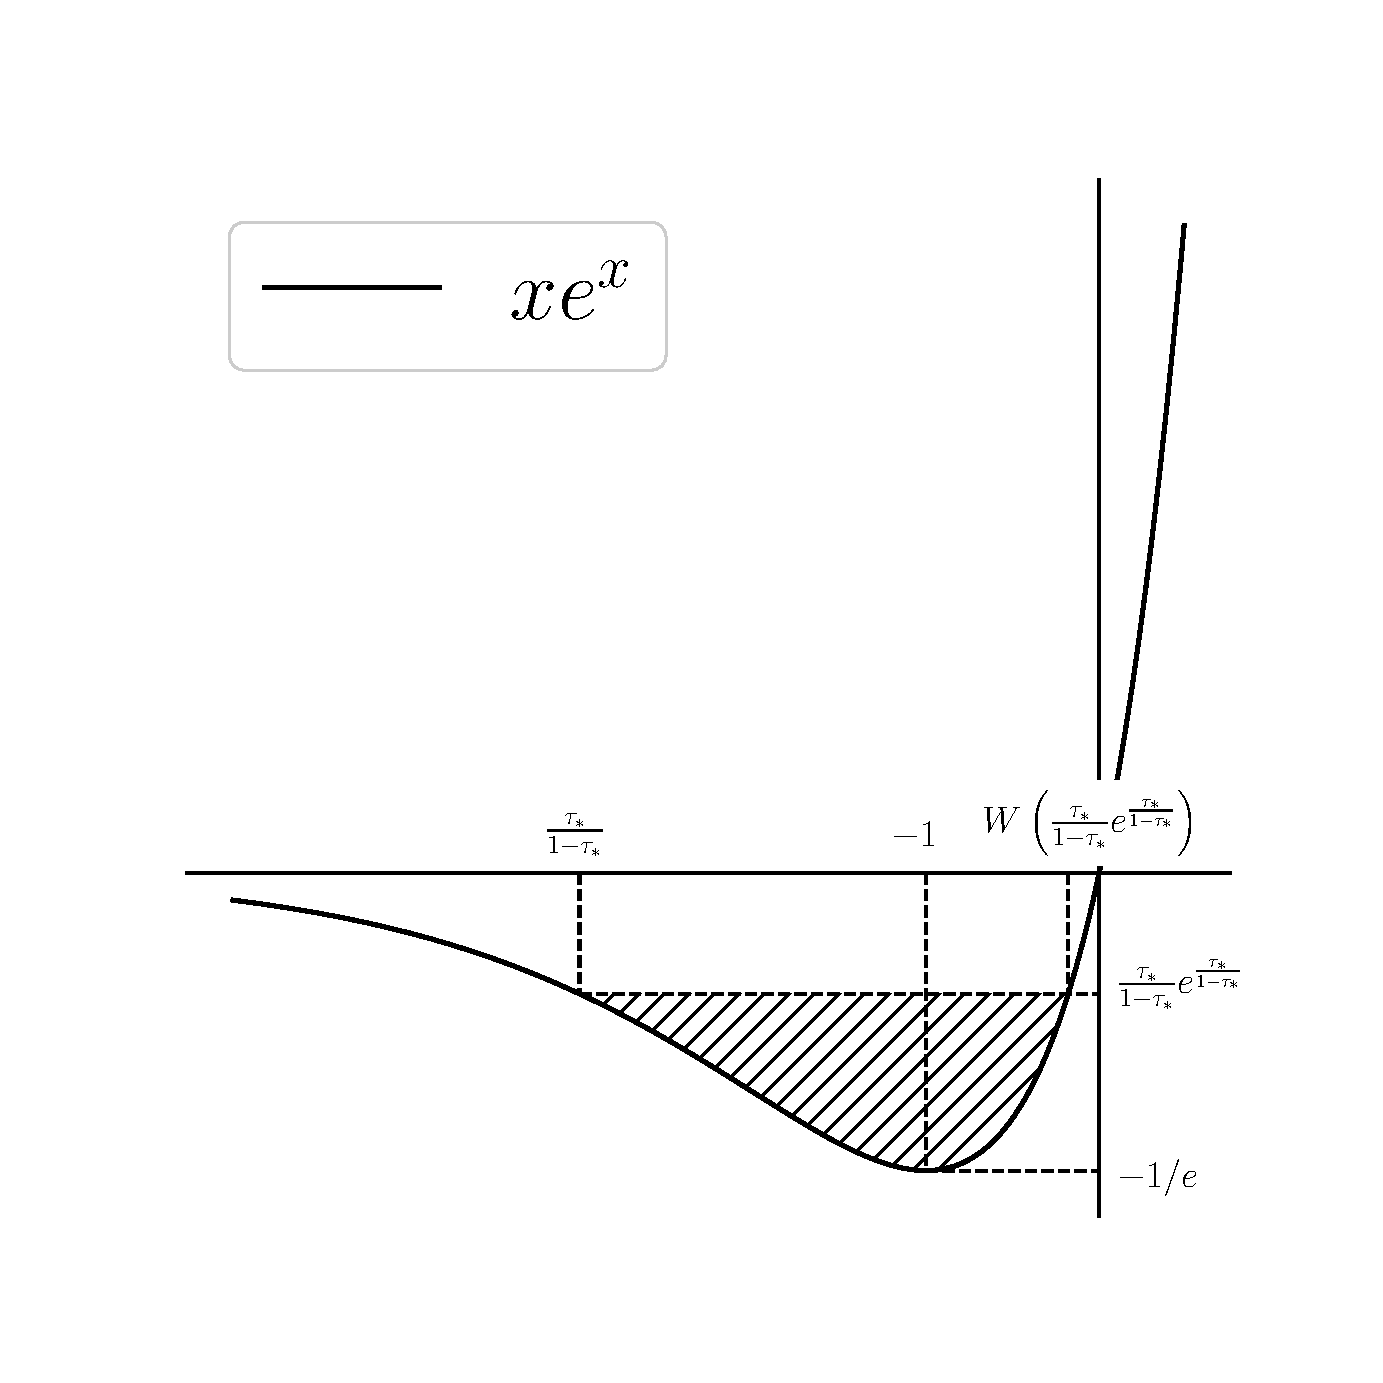
\includegraphics[width=0.7\textwidth]{images/w_inverse.eps}
		\caption{Функция $f(x) = x e^x$ убывает при $x < -1$ и возрастает при $x > -1$. На рисунке изображена область, соответствующая неравенству \eqref{eq:phi_double_inequality}.}
		\label{fig:w_inverse}
	\end{figure}
	
	Также заметим, что равенство выполняется только в точке $\beta = \tilde{\beta}(\tau_*)$.
	
\end{proof}

Теперь проанализируем условия \eqref{eq:step_3_cond_phi} и \eqref{eq:step_3_cond_2}. По утверждениям \ref{prop:phi_theta}, \ref{prop:delta_theta} и \ref{prop:delta_phi},
\begin{equation}
	\begin{cases}
		\delta(\beta, \tau_*) < \phi(\beta) < \theta(\beta, \tau_*), & \beta < \tilde{\beta}(\tau_*),\\
		\delta(\beta, \tau_*) = \phi(\beta) = \theta(\beta, \tau_*), & \beta = \tilde{\beta}(\tau_*),\\
		\delta(\beta, \tau_*) > \phi(\beta) > \theta(\beta, \tau_*), & \beta > \tilde{\beta}(\tau_*).
	\end{cases}
\end{equation}
%
Тогда условия \eqref{eq:step_3_cond_phi} и \eqref{eq:step_3_cond_2} можно представить в упрощённом виде:
\begin{equation}
	\label{eq:phi_theta_cond}
	\begin{cases}
		\alpha \geq \theta(\beta, \tau_*), & \beta \leq \tilde{\beta}(\tau_*),\\
		\alpha \geq \phi(\beta), & \beta > \tilde{\beta}(\tau_*).
	\end{cases}
\end{equation}


На рисунке \ref{fig:step3_t1} изображена область параметров для различных фиксированных значений $\tau_*$.

\begin{figure}
	\centering
	\begin{minipage}{.45\linewidth}
		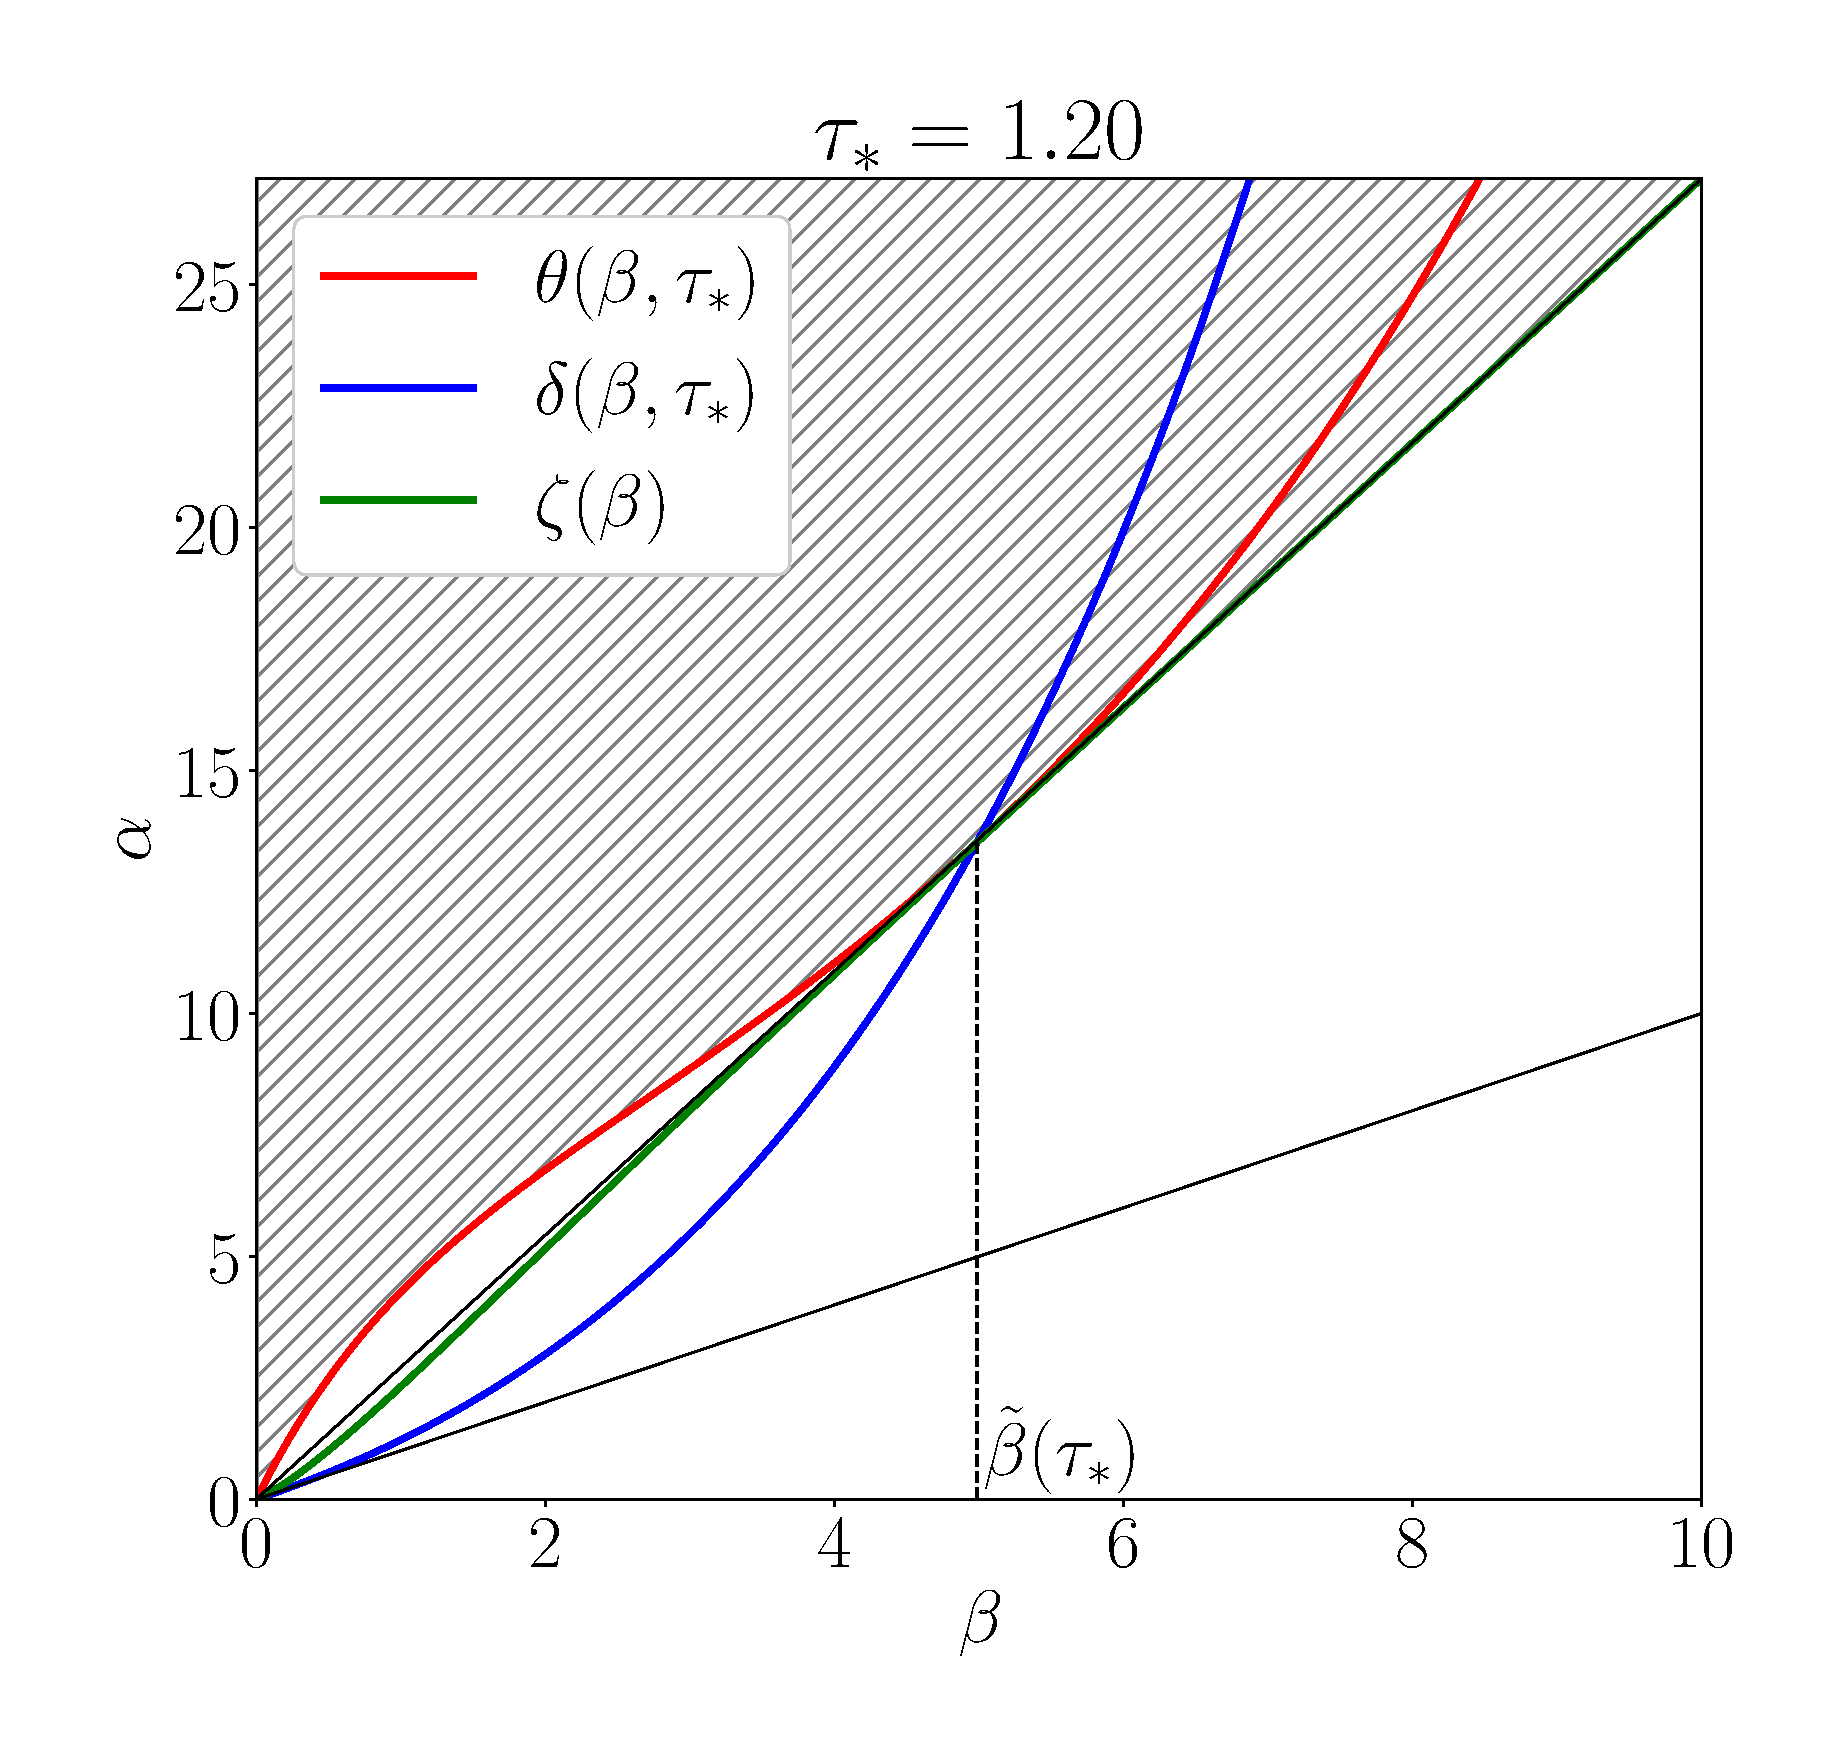
\includegraphics[width=\linewidth]{images/conditions_tau_1p20.eps}
	\end{minipage}
	\hspace{.05\linewidth}
	\begin{minipage}{.45\linewidth}
		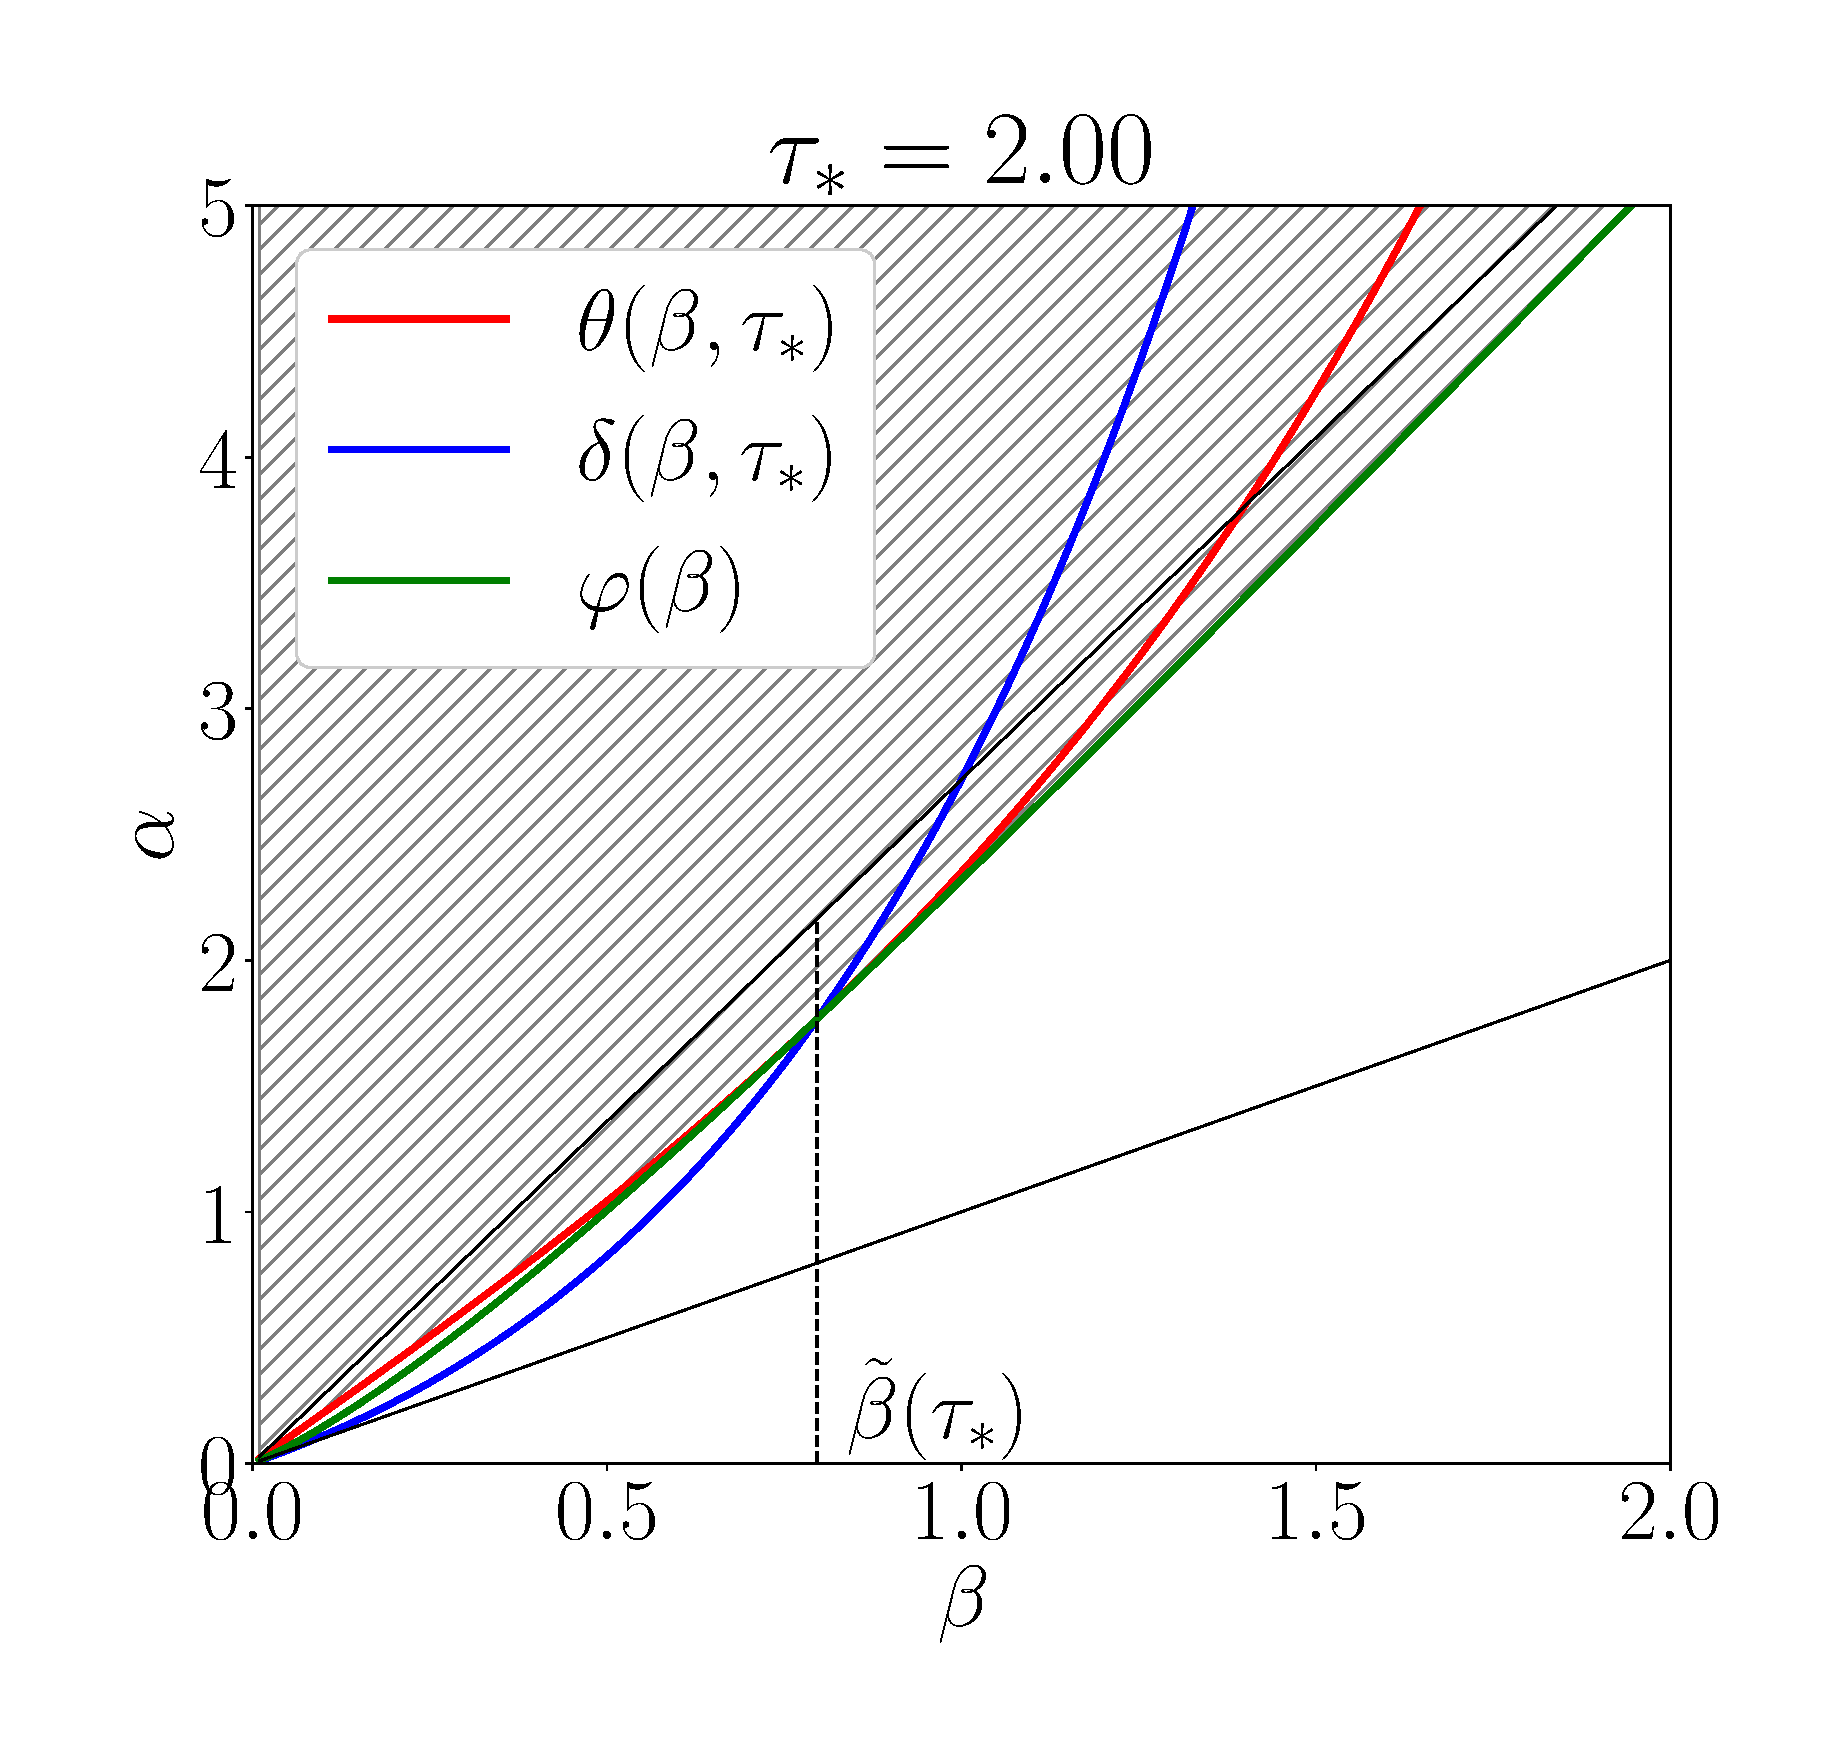
\includegraphics[width=\linewidth]{images/conditions_tau_2p00.eps}
	\end{minipage}
	\caption{Иллюстрация области параметров \eqref{eq:phi_theta_cond} при различных значениях $\tau_*$. Помимо функций $\theta$, $\varphi$ и $\delta$, на рисунках присутствуют прямые $\alpha = \beta$ и $\alpha = e\beta$.}
	\label{fig:step3_t1}
\end{figure}

Заметим, что при фиксированных $\beta$ и $\tau_*$ ограничение на $\alpha$ формулируется в виде $\alpha \geq c$ для некоторой константы $c$. Это будет важно в дальнейшем, когда мы будем искать параметры, удовлетворяющие уравнению \eqref{eq:period_equation}.


\subsection{Доказательство периодичности построенного решения}
В разделе \ref{sec:ch2/sect2/subsect_aux_result} на промежутке $[0,t_2]$ построено решение уравнения \eqref{eq:mg_relay_w} с начальной функцией из множества \eqref{eq:mg_init_set}. Показано, что оно совпадает с функцией $u_*(t)$, которая описывается формулами \eqref{eq:u_step1}, \eqref{eq:u_step2}, \eqref{eq:u_step3}, \eqref{eq:u_step4}. Для доказательства того, что получено периодическое решение с периодом $T = t_2 - t_0$, достаточно убедиться в том, что расстояние между точками $t_1$ и $t_2$ не меньше длины наибольшего запаздывания $\tau_m$. Для этого проследим за изменением функции $w(t)$ на промежутке $[t_1,t_1+\tau_m]$ и покажем, что на данном промежутке сохраняется неравенство $w(t) > 1$.

\subsection{Анализ функции $w(t)$}

\begin{proposition}
	\label{w>1_t_1-t_1+1} Пусть выполнено \eqref{eq:cond_th_w>1_t_1+1},
	\begin{equation}
		\label{w>1_t_1+1}
		e^{\beta s_*}\left(s_*(1-e^\beta) + e^\beta \right) - 1 > 0,
	\end{equation}
	тогда функция $w(t)>1$ при $t\in (t_1, t_1 + 1]$.
\end{proposition}
\begin{proof}
	Неравенство $w(t)>1$ на промежутке $(t_1, t_1 + 1]$ с учетом $u_0 A = e^{\beta t_0}$ эквивалентно неравенству $u_0Ae^{-\beta t}(1+\alpha e^{\beta }(t-t_0-1)) >1$ или $1+\alpha e^{\beta }(t-t_0-1) > e^{\beta (t-t_0)}$.
	Заметим, что в левой части неравенства стоит аффинная функция, в правой --- экспоненциальная (выпуклая функция). Тогда для верности утверждения на $(t_1, t_1 + 1)$ достаточно, чтобы функция $w(t)$ была больше или равна $1$ в концах соответствующего отрезка. Известно, что $w(t_1) = 1$, остается проверить $w(t_1+1) \geqslant 1$. Теперь добавим, что для верности утверждения на полуинтервале $(t_1, t_1 + 1]$ последнее условие нужно усилить строгим знаком.
	Запишем это в виде:
	$$w(t_1+1) = e^{-\beta (t_1 -t_0+ 1)}( 1+\alpha e^{\beta }(t_1-t_0) )>1 .$$
	Используя равенство $\alpha = \dfrac{e^{\beta(t_1 - t_0)}-1}{e^\beta(t_1 - t_0 -1)}$, которое следует из $w(t_1)=1$, перепишем неравенство:
	$$e^{-\beta(t_1-t_0+1)}\Big(1 + \dfrac{e^{\beta(t_1 - t_0)}-1}{e^\beta(t_1 - t_0 -1)}e^\beta(t_1 - t_0) \Big)>1.$$
	После эквивалентных преобразований получим \eqref{eq:cond_th_w>1_t_1+1}.
\end{proof}

Функция $w(t)$ изменяется в точках переключения функции $u_*(t)$, к которым прибавляются все возможные запаздывания, а именно в точках из множеств
%
\[E_*\stackrel{\text{def}}{=}\{t_0 + \tau_k\},\ E_{**}\stackrel{\text{def}}{=}\{t_0 + 1 + \tau_k\},\ E_{***}\stackrel{\text{def}}{=}\{t_1 + \tau_k\},\text{ где }k=0,1,\ldots,m,\ \tau_0=1.\]
%
Отметим, что данные множества точек могут пересекаться.

Определим функции 
$$\xi(s)\stackrel{\text{def}}{=}\alpha e^{-\beta s} s ,\quad \eta(s)\stackrel{\text{def}}{=}\frac{\alpha^2}{2} e^{-\beta( s-1)} (s-1)^2$$
\begin{lemma}
	\label{lm:lem_w_*}
	При переходе через точки из множеств $E_*$, $E_{**}$, $E_{***}$ функция $w(t)$ изменяется следующим образом:
	\begin{equation}
		\label{eq:w_*}
		w(t_0 + \tau_k+0) = w(t_0 + \tau_k-0) +  \xi(t-\tau_k-t_0),
	\end{equation}
	\begin{equation}
		\label{eq:w_**}
		w(t_0 +1+ \tau_k+0) = w(t_0 +1+ \tau_k-0) +\eta(t-\tau_k-t_0), 
	\end{equation}
	\begin{equation}
		\label{eq:w_***} 
		w(t_1 + \tau_k+0) = w(t_1 + \tau_k-0)-\xi(t-\tau_k-t_0)-\eta(t-\tau_k-t_0)+
		(u_1 e^{\beta t_1}-u_0)e^{-\beta(t-\tau_k)}.
	\end{equation}
	Причем, если точка переключения принадлежит нескольким множествам, то применяются несколько  соответствующих формул одновременно.
\end{lemma}

\begin{proof}
	
	Рассмотрим переход через точку из множества $E_*$. В точке $t_0 + \tau_k$ слагаемое $u(t - \tau_k)$ изменяет форму с \eqref{eq:step1} %$u(t-h) = u_0e^{-\beta( t - h)}$ 
	на \eqref{eq:step2}. %$u(t-h) = u_0 e^{-\beta( t-h)}(\alpha A(t-h - t_0)+1)$.
	Следовательно, функция $w(t)$ при переходе через $t_0 + \tau_k$ изменяется на разность:
	% 
	\[u_0 e^{-\beta( t-\tau_k)}(\alpha A(t - \tau_k - t_0)+1) - u_0e^{-\beta( t - \tau_k)}= \alpha e^{-\beta( t-\tau_k-t_0)}(t-\tau_k-t_0).\]
	%, что указано в выражении \eqref{w_*} Леммы \ref{lem_w_*}. 
	%
	% Можно и расписать подробно
	Аналогично доказываются формулы \eqref{eq:w_**} и \eqref{eq:w_***}. При рассмотрении точек из множеств $E_{**}$ и $E_{***}$ происходит изменение аналитической формы одного из слагаемых с \eqref{eq:u_step2} на \eqref{eq:u_step3} и с \eqref{eq:u_step3} на \eqref{eq:u_step4} соответственно.
	
	Отдельно разберем ситуацию, когда некоторые из точек множеств $E_*$, $E_{**}$ и $E_{***}$ совпали. Заметим, что точки внутри множеств совпадать не могут, так как все запаздывания различны. Так же не могут совпадать точки из разных множеств с прибавлением одинакового запаздывания, так как точки $t_0$, $t_0 + 1$ и $t_1$ различны. Тогда совпасть могут только точки из разных множеств  с прибавлением разных запаздываний. Следовательно, изменение функции $w(t)$ в совпадающих точках будут происходить за счет разных слагаемых $u(t-\tau_k)$, а значит, независимо друг от друга. Тогда общее изменение функции $w(t)$ будет складываться из суммы изменений вида \eqref{eq:w_*}, \eqref{eq:w_**} и \eqref{eq:w_***}.
\end{proof}


Отметим, что добавки в формулах \eqref{eq:w_*}, \eqref{eq:w_**} неотрицательны и обращаются в ноль в соответствующих точках переключения.

\begin{lemma}
	\label{lm:lem_w>1}
	Пусть выполнены условия лемм \ref{lm:t1_existence}, \ref{lm:t1_locate} и пусть, кроме того,
	параметры удовлетворяют ограничениям \eqref{eq:cond_th_w>1_t_1+1}, \eqref{eq:cond_hair_hair_01}, \eqref{eq:cond_hair_hair_02}, \eqref{eq:cond_hair_hair_1}.
	Тогда $w(t)>1$ при $t\in(t_1,t_1+\tau_m]$.
\end{lemma}

\subsubsection{Доказательство леммы \ref{lm:lem_w>1}}
Идея доказательства состоит в следующем. На каждом из промежутков $(t_1, t_1+\tau_k]$ мы определим функцию $\tilde{v}(t) < w(t)$ и покажем, что $1 < \tilde{v}(t)$. Тем самым, утверждение леммы \ref{lm:lem_w>1} окажется доказано.

Будем последовательно рассматривать промежутки $(t_1,t_1+1]$, $(t_1+\tau_{k-1},t_1+\tau_k]$, $k = 1,\ldots,m$. Доказывая на каждом шаге, что на соответствующем промежутке верно $w(t) > 1$, мы также доказываем, что на нём не появится новых точек переключения. Поэтому нам не потребуется рассматривать изменения функции $w(t)$, отличные от тех, что описаны в лемме \ref{lm:lem_w_*}.

Рассмотрим вспомогательную функцию $\tilde{u}(t)$, определенную на отрезке $[0,t_2]$ следующим образом (см. рис. \ref{fig:u_hair}): 
\begin{equation}
	\label{eq:u_hair}
	\tilde{u}(t)\stackrel{\text{def}}{=}\left\lbrace\begin{array}{cl}
		u_0e^{-\beta t} & \text{ при } t\in[0,t_1],
		\\
		u_1e^{-\beta (t-t_1)} & \text{ при } t\in(t_1,t_1+1+\tau_m].
	\end{array}\right.
\end{equation}
%
%%% ГРАФИК U-КУДРЯВОЕ
\begin{figure}
	\centering
	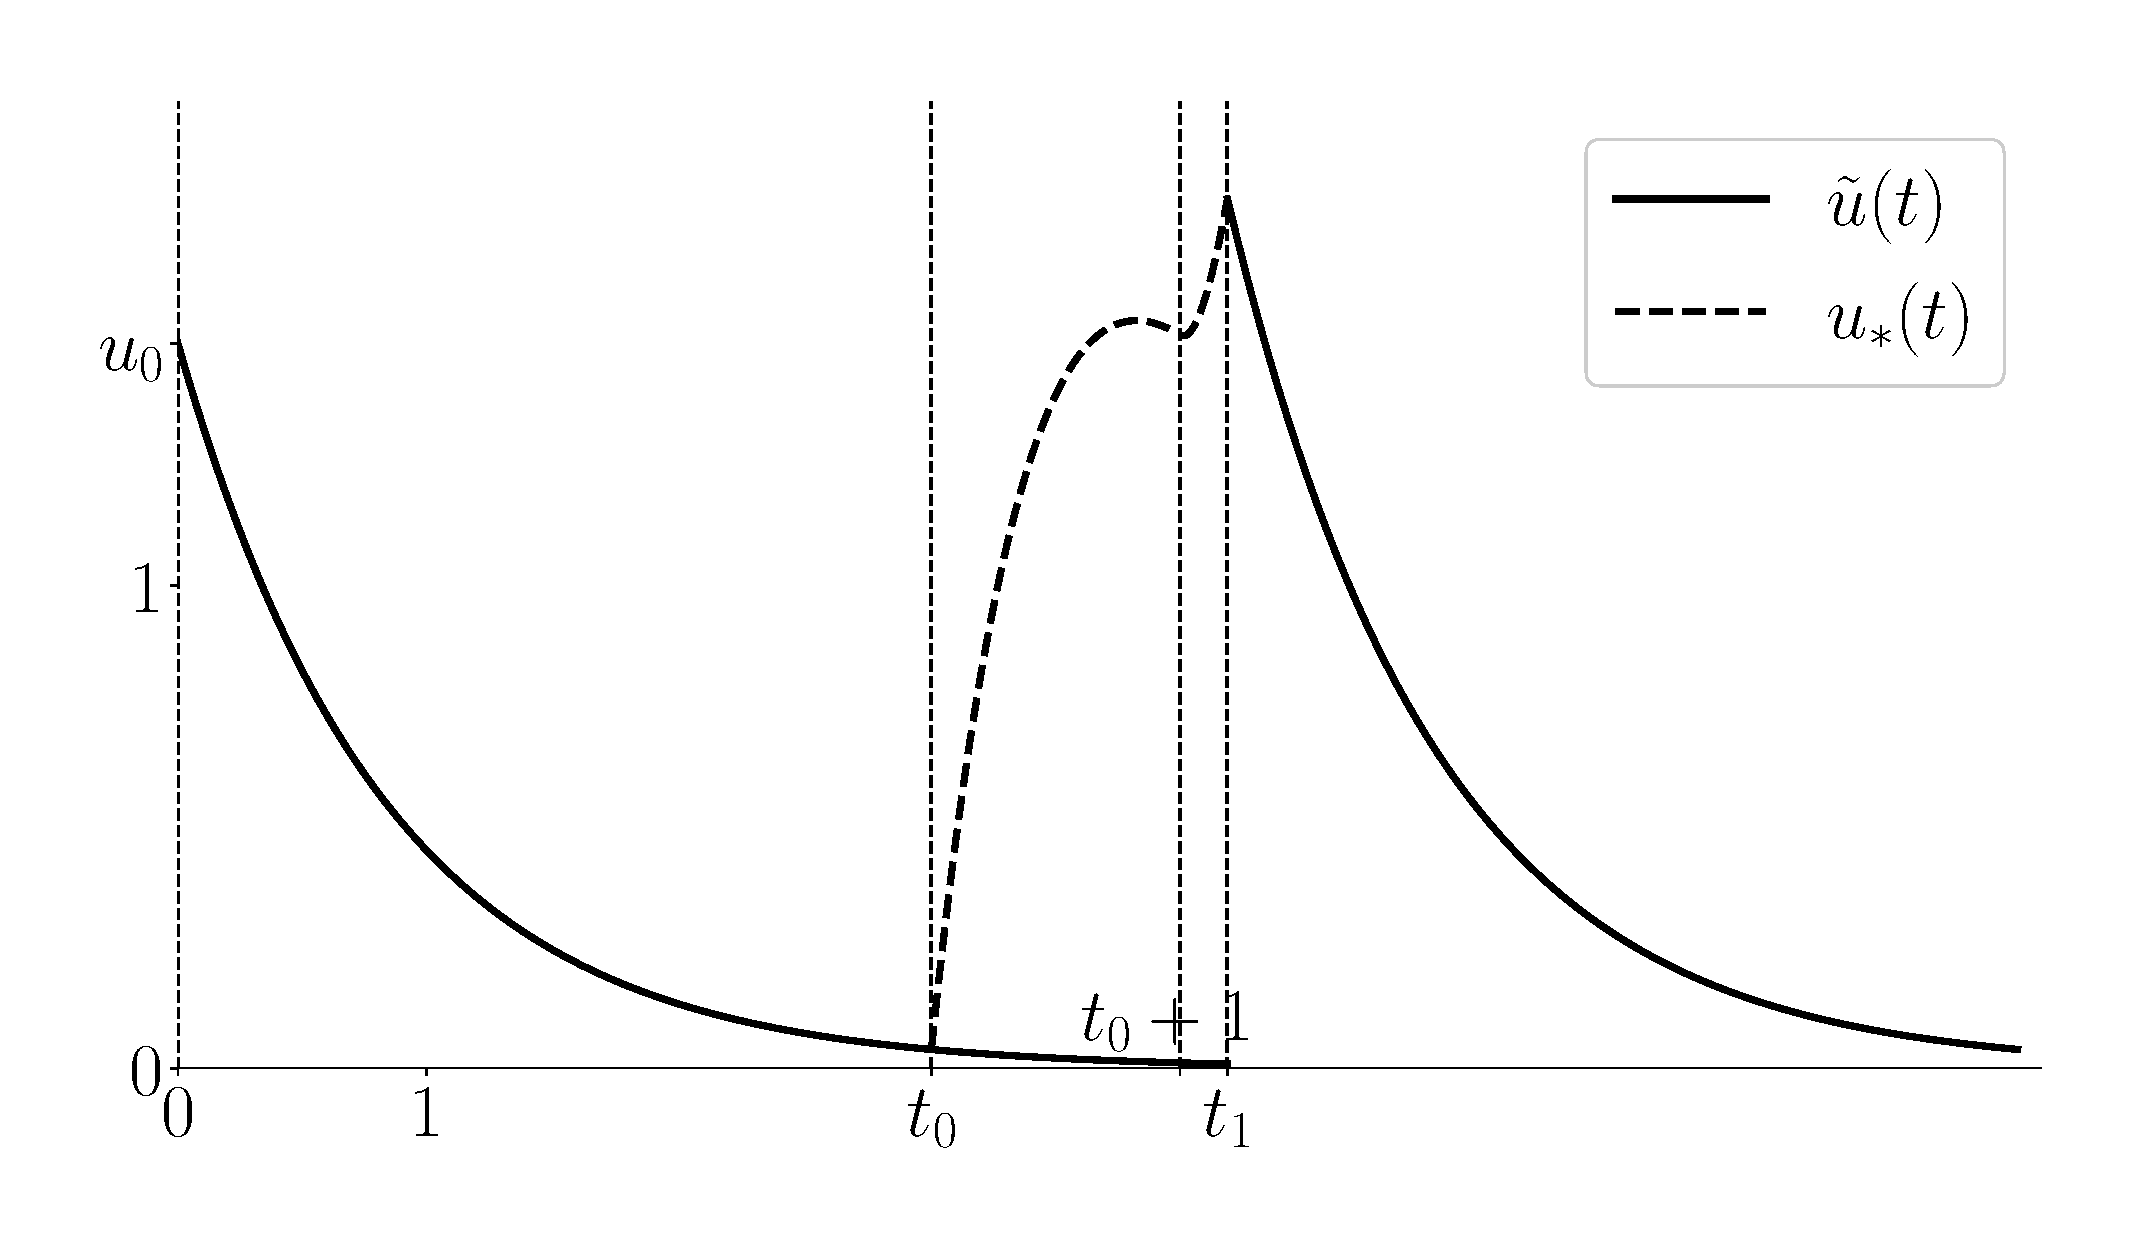
\includegraphics[width=0.7\textwidth]{u_hair.eps}
	\caption{Схематичный график функции $\tilde{u}(t)$}
	\label{fig:u_hair}
\end{figure}
%

По функции $\tilde{u}(t)$ построим функцию
%
\[
\tilde{w}(t) = \sum_{i=0}^{m}\tilde{u}(t-\tau_i),
\]
%
определенную на отрезке $[\tau_m, t_1 + \tau_m]$. Ее явный аналитический вид:
%
\begin{equation}
	\label{eq:w_hair}
	\tilde{w}(t)=
	\begin{cases}
		e^{-\beta (t-t_0)} & \text{ при } t\in[\tau_m,t_1+1],\\
		C_k e^{-\beta(t-t_0)} & \text{ при } t\in(t_1 + \tau_{k-1}, t_1 + \tau_k],\ k=1,\ldots,m,
	\end{cases}
\end{equation}
где
\[C_k = 1+\left(\frac{\alpha^2}{2}e^\beta\big( s_*-1)^2+\alpha s_*\right)\sum_{i=0}^{k-1}e^{\beta \tau_i}.\]

Функция $\tilde{w}(t)$ обладает скачками в точках %$t_1 + \tau_k$ 
множества $E_{***}$:
\begin{equation}
	\label{eq:w_hair_***} 
	\tilde{w}(t_1 + \tau_k+0) = \tilde{w}(t_1 + \tau_k-0)+
	e^{-\beta(t-\tau_k)}(u_1 e^{\beta t_1}-u_0).
\end{equation}
%
Изменение \eqref{eq:w_hair_***} функции $\tilde{w}(t)$ --- это \eqref{eq:w_***} без участия слагаемых-добавок из \eqref{eq:w_*} и \eqref{eq:w_**}. В отличие от $w(t)$, функция $\tilde{w}(t)$ не меняет форму при переходе через точки из множеств $E_*$ и $E_{**}$. Заметим также, что функция $\tilde{w}(t)$ будет разрывной в точках из $E_{***}$. Схематичный график функции $\tilde{w}(t)$ изображен на рисунке \ref{fig:w_hair}.

Теперь к этой функции <<добавим>> на отрезках $[t_0+1,t_1+1]$, $[t_0+\tau_k, t_1+\tau_k]\cap[t_1+\tau_{k-1},t_1+\tau_k]$, $k=1,\ldots,m$, слагаемые из \eqref{eq:w_*}.

Пусть
%
\[
\tilde{\xi}(s) = 
\begin{cases}
	\xi(s) & \text{ при } s\in[0,s_*],\\
	0 & \text{ при } s\notin[0,s_*].
\end{cases}
\]
%
Определим функцию $\tilde{v}(t)$ на отрезке $[\tau_m,t_1+1+\tau_m]$ следующим образом (см. рис. \ref{fig:w_hair}):
%
\[
\tilde{v}(t) =
\begin{cases}
	\tilde{w}(t)+\tilde{\xi}(t-t_0-1)& \text{ при } t\in[\tau_{m}, t_1 + 1],\\
	\tilde{w}(t)+\tilde{\xi}(t-t_0-\tau_k)& \text{ при } t\in(t_1 + \tau_{k-1}, t_1 + \tau_k],\
\end{cases}
\]
%
%
%%% ГРАФИК W-КУДРЯВОЕ и V-КУДРЯВОЕ
\begin{figure}
	\label{fig:w_hair}
	\centering
	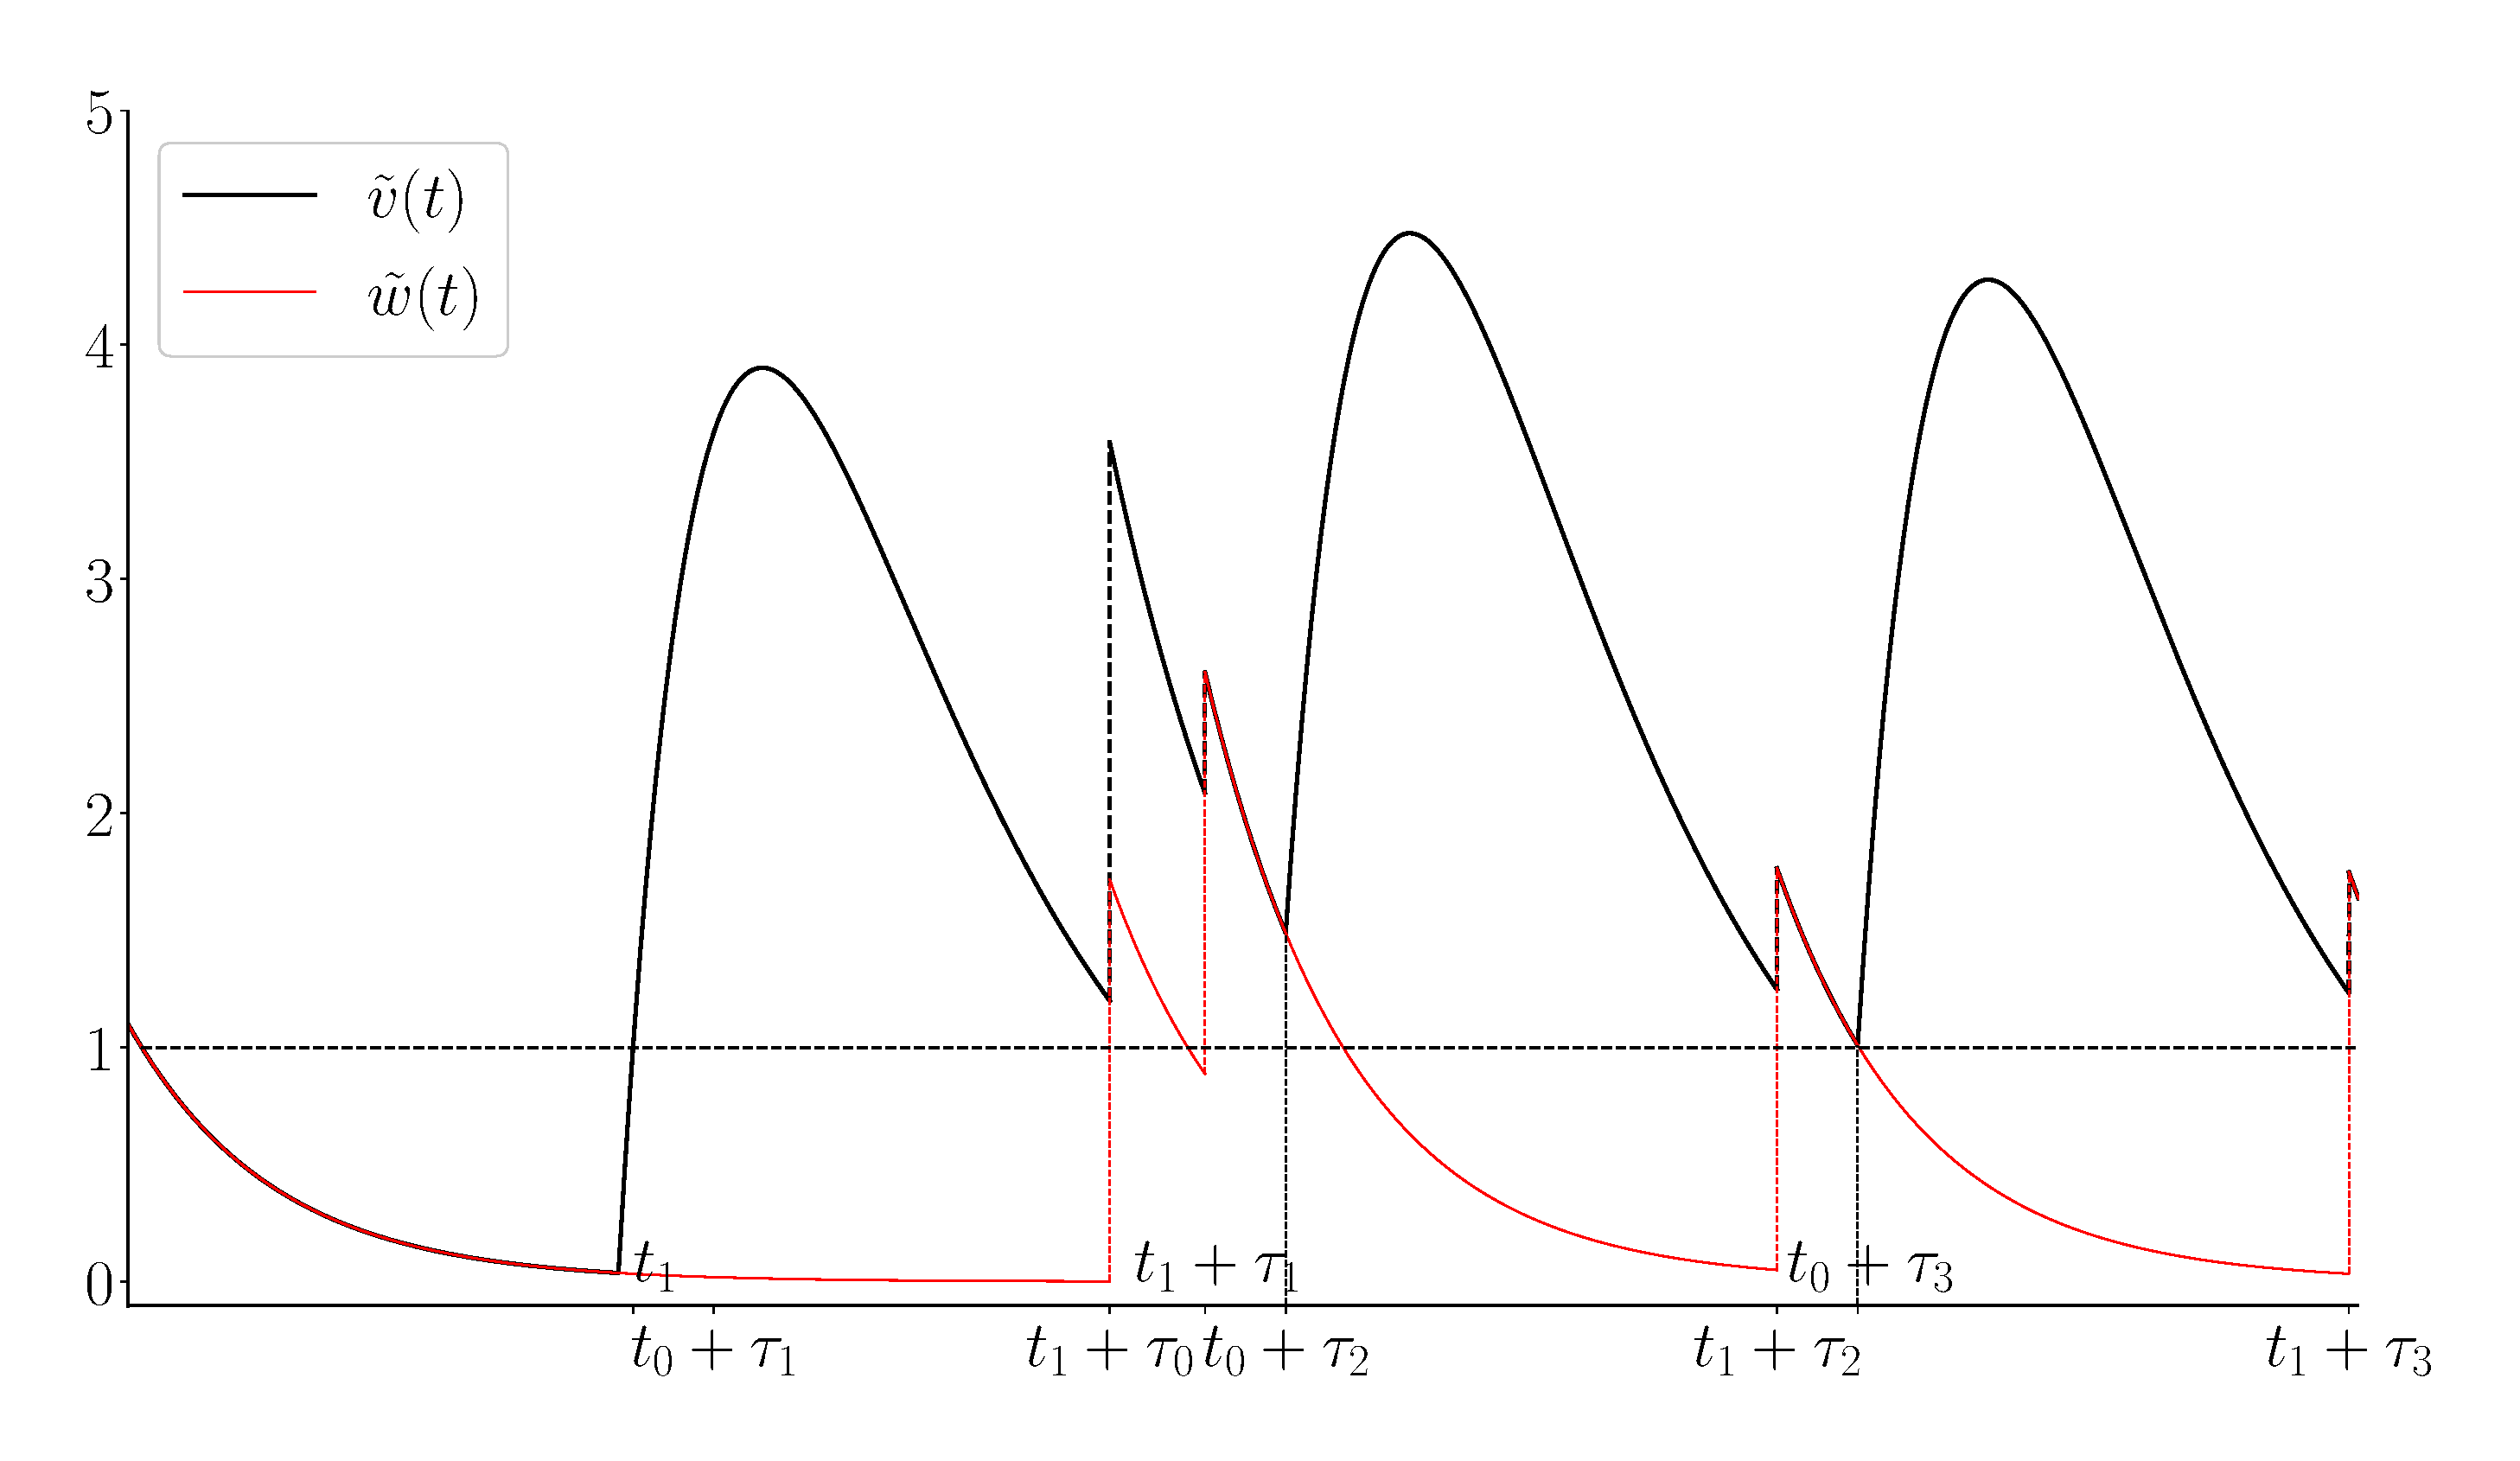
\includegraphics[width=0.7\textwidth]{w_hair.eps}
	\caption{Схематичный график функций $\tilde{w}(t)$ и $\tilde{v}(t)$. На этом рисунке $t_0+\tau_1 \notin[t_1+\tau_0,t_1+\tau_1]$, поэтому при $t\in(t_1+\tau_0,t_1+\tau_1]$ функция  $\tilde{v}(t)$ описывается формулой \eqref{eq:v_hair1} при $k=1$, и соответствующие условия того, что здесь $\tilde{v}(t)>1$, --- это формулы \eqref{eq:cond_hair_hair_02} и \eqref{eq:cond_hair_hair_1} при $k=1$. На следующем отрезке $[t_1+\tau_1,t_1+\tau_2]$ другая ситуация,  $t_0+\tau_2\in[t_1+\tau_1,t_1+\tau_2]$, поэтому здесь $\tilde{v}(t)$ описывается формулой \eqref{eq:v_hair2} при $k=2$, а соответствующие условия для $\tilde{v}(t)>1$ здесь --- это \eqref{eq:cond_hair_hair_01} и \eqref{eq:cond_hair_hair_1} при $k=2$. }
\end{figure}
%

%
\begin{proposition}
	\label{prop:w_w_hair}
	$\tilde{w}(t)\leqslant\tilde{v}(t)\leqslant w(t)$ при $t\in[\tau_m,t_1+\tau_k]$.
\end{proposition}
\begin{proof}
	Функции $\tilde{w}(t)$ и $\tilde{v}(t)$ отличаются на неотрицательные добавки \eqref{eq:w_*}, функции $\tilde{v}(t)$ и $w(t)$ отличаются по крайней мере на неотрицательные добавки \eqref{eq:w_**}.
\end{proof}

\begin{proposition}
	\label{prop:v_hair>1}
	Пусть выполнены условия лемм \ref{lm:t1_existence}, \ref{lm:t1_locate} и ограничения \eqref{eq:cond_th_w>1_t_1+1}, \eqref{eq:cond_hair_hair_01}, \eqref{eq:cond_hair_hair_02}, \eqref{eq:cond_hair_hair_1}. Тогда 
	$\tilde{v}(t)>1$ при $t\in(t_1,\ t_1+\tau_m]$.
\end{proposition}

\begin{proof}
	Опишем $\tilde{v}(t)$ в явном виде.
	%
	\[
	\tilde{v}(t) = 
	\begin{cases}
		e^{-\beta(t-t_0)} & \text{ при } t\in[\tau_m,t_0+1],\\
		e^{-\beta(t-t_0)}+\alpha e^{-\beta (t-t_0-1)} (t-t_0-1) & \text{ при } t\in(t_0+1,t_1+1].
	\end{cases}
	\]
	%
	В зависимости от упорядоченности пары точек $t_0+\tau_k$ и $t_1+\tau_{k-1}$ возможны два варианта аналитического описания функции $\tilde{v}(t)$ на отрезке $[t_1+\tau_{k-1},t_1+\tau_k]$:
	\begin{enumerate}
		\item[1)] если $t_0+\tau_k\in[t_1+\tau_{k-1},t_1+\tau_k]$, то
		\begin{equation}
			\label{eq:v_hair1}
			\tilde{v}(t)=
			\begin{cases}
				C_k e^{-\beta(t-t_0)} & \text{ при } t\in(t_1+\tau_{k-1},t_0+\tau_k],\\
				C_k e^{-\beta(t-t_0)} + \alpha e^{-\beta (t-t_0-\tau_k)} (t-t_0-\tau_k) & \text{ при } t\in(t_0+\tau_k,t_1+\tau_k];
			\end{cases}
		\end{equation}
		
		\item[2)] если $t_0+\tau_{k} < t_1+\tau_{k-1}$, то
		\begin{equation}
			\label{eq:v_hair2} 
			\tilde{v}(t)= C_k e^{-\beta(t-t_0)}+\alpha e^{-\beta (t-t_0-\tau_k)} (t-t_0-\tau_k) \text{ при } t\in(t_1+\tau_{k-1},t_1+\tau_k].
		\end{equation}
	\end{enumerate}
	
	% Сделаем замену $t=t(s)=s+\tau_k+t_0$. %Учитывая, что $u_0A=e^{\beta t_0}$, 
	% Тогда
	% \begin{enumerate}
		%     \item[1)] если $s_*\leqslant \tau_{k}-\tau_{k-1}$, то
		%     $$\tilde{v}(t(s))=\left\lbrace\begin{array}{cl}
			% C_ke^{-\beta \tau_k}e^{-\beta s} & \text{ при } t\in[s_*+\tau_{k-1}-\tau_k,0],
			% \\
			% e^{-\beta s}(\alpha s+C_ke^{-\beta \tau_k}) & \text{ при } t\in(0,s_*];
			% \end{array}\right.$$
		%     \item[2)] если $s_*>\tau_{k}-\tau_{k-1}$, то
		%     $$\tilde{v}(t(s))=e^{-\beta s}(\alpha s+C_ke^{-\beta \tau_k})  \text{ при } t\in(s_*+\tau_{k-1}-\tau_k,s_*].$$
		% \end{enumerate}
	
	Функция $C_ke^{-\beta s}$ убывает по $s$.
	
	Функция $C_ke^{-\beta \tau_k}e^{-\beta s}+\alpha e^{-\beta s} s$ обладает локальным максимумом в точке $\dfrac{\alpha-\beta C_ke^{-\beta \tau_k}}{\alpha \beta}$.
	%
	%Функция $e^{-\beta s}(\frac{\alpha^2}{2}e^\beta\big( s_*-1)^2+\alpha s_*+C_k)$ либо монотонно убывает, либо имеет локальные минимум и максимум. В последнем случае точка минимума оказывается меньше 1.
	%
	Тогда на любом конечном промежутке она либо монотонна, либо имеет локальный максимум, то есть достаточно проверять неравенство в концах промежутка. Это означает, что для верности неравенства $\tilde{v}(t)>1$ при $t\in(t_1,t_1+1]$ и  $t\in(t_1+\tau_{k-1},t_1+\tau_k]$, $k = 1,\ldots,m$,  достаточно, чтобы выполнялось  
	\begin{equation}
		\label{eq:cond_v_hair>1_1}
		e^{-\beta(t-t_0)}+\alpha e^{-\beta (t-t_0-1)} (t-t_0-1)|_{t=t_1}\geqslant 1,
	\end{equation}
	\begin{equation}
		\label{eq:cond_v_hair>1_2}
		e^{-\beta(t-t_0)}+\alpha e^{-\beta (t-t_0-1)} (t-t_0-1)|_{t=t_1+1}>1,
	\end{equation}
	\begin{equation}
		\label{eq:cond_v_hair>1_3}
		C_k e^{-\beta(t-t_0)}+\alpha e^{-\beta (t-t_0-\tau_k)} (t-t_0-\tau_k)|_{t=\max\{t_0+\tau_k,t_1+\tau_{k-1}\}}>1,
	\end{equation}
	\begin{equation}
		\label{eq:cond_v_hair>1_4}
		C_k e^{-\beta(t-t_0)}+\alpha e^{-\beta (t-t_0-\tau_k)} (t-t_0-\tau_k)|_{t=t_1+\tau_k}>1.
	\end{equation}
	Неравенство \eqref{eq:cond_v_hair>1_1} справедливо и обращается в равенство, поскольку $s_*=t_1-t_0$ --- это корень уравнения $e^{\beta s}-1=\alpha e^{\beta}(s-1)$. Неравенство \eqref{eq:cond_v_hair>1_2} эквивалентно \eqref{eq:cond_th_w>1_t_1+1}. Неравенство \eqref{eq:cond_v_hair>1_3} при $t_0+\tau_k\geqslant t_1+\tau_{k-1}$ обращается в \eqref{eq:cond_hair_hair_01}. При при $t_0+\tau_k<t_1+\tau_{k-1}$ это неравенство заменим более сильным
	\[C_ke^{-\beta(t-t_0)}|_{t=t_1+\tau_{k-1}}>1,\]
	которое эквивалентно \eqref{eq:cond_hair_hair_02}.
	Неравенство \eqref{eq:cond_v_hair>1_4} эквивалентно \eqref{eq:cond_hair_hair_1}.
	
	% Отметим, что неравенство (\ref{cond_hair_hair_02}) при $k=1$ заменяется более слабым, но достаточным неравенством (\ref{cond_th_w>1_t_1+1}), гарантирующим, что 
	% \begin{figure}
		%     \centering
		%     \includegraphics[width=0.7\textwidth]{w_hair_k.png}
		%     \caption{Схематичный график функции $\tilde{w}_k(t)$}
		%     \label{pic:w_hair}
		% \end{figure}
\end{proof}

Справедливость леммы \ref{lm:lem_w>1} следует из утверждений \ref{prop:w_w_hair} и \ref{prop:v_hair>1}.

\section{Дискретные бегущие волны}\label{sec:ch2/sect3}

Докажем, что при фиксированных параметрах $\alpha, \beta$ и некотором $\Delta$ существует периодическое решение системы \eqref{eq:mg_relay_1} с периодом $T(\Delta)$, удовлетворяющее уравнению \eqref{eq:period_equation} при $p = 1$.

Пусть $\Delta > 1$, тогда запаздывания равны $\{1, \Delta, 2\Delta, \ldots, m\Delta\}$. В этом случае нормировка \eqref{eq:mg_norm} не изменяет уравнение периодов \eqref{eq:period_equation}.  Подставим значение $T(\Delta)$ из \eqref{eq:mg_period_T} в \eqref{eq:period_equation} при $p = 1$:
%
\begin{equation}
	\label{eq:period_eq}
	\dfrac{1}{\beta}\ln\left( \frac{\alpha^2}{2}Ae^{\beta}( s_*-1)^2+\alpha A s_* + 1\right) = \Delta (m + 1).
\end{equation}
%
Элементарными преобразованиями сводим уравнение к виду:
\begin{equation}
	\label{eq:period_eq_exp}
	\dfrac{1}{A}\left(e^{\beta\Delta(m + 1)} - 1\right) = \dfrac{\alpha^2}{2}e^{\beta}( s_* - 1)^2 + \alpha s_*.
\end{equation}

\begin{proposition}
	$\lim\limits_{\alpha\to+\infty} s_*(\alpha) = 1 + 0$.
\end{proposition}
\begin{proof}
	Значение $s_*$ находится как меньший корень уравнения $\alpha = \theta(\beta, s_*)$. В утверждении \ref{prop:phi_theta} было показано, что при фиксированном $\beta$ у функции $\theta(\beta,  s_*)$ ровно одна точка минимума $ s_*^{\text{min}}$ (см. рисунок \ref{fig:theta_func_min}), при этом
	%
	\begin{equation}
		\lim\limits_{s_* \to 1+0} \theta(\beta, s_*) = \lim\limits_{s_*\to +\infty} \theta(\beta,  s_*) = +\infty.
	\end{equation}
	%
	Тогда у функции $s_*(\alpha)$ две непрерывных ветви $s_* \in (1;  s_*^{\text{min}}]$ и $ s_* \in [ s_*^{\text{min}}; +\infty)$. Меньший корень лежит на левой ветви, но тогда $\lim\limits_{\alpha\to+\infty} s_*(\alpha)= 1 + 0$.
\end{proof}
%
%%% ФУНКЦИЯ THETA
\begin{figure}
	\label{fig:theta_func_min}
	\centering
	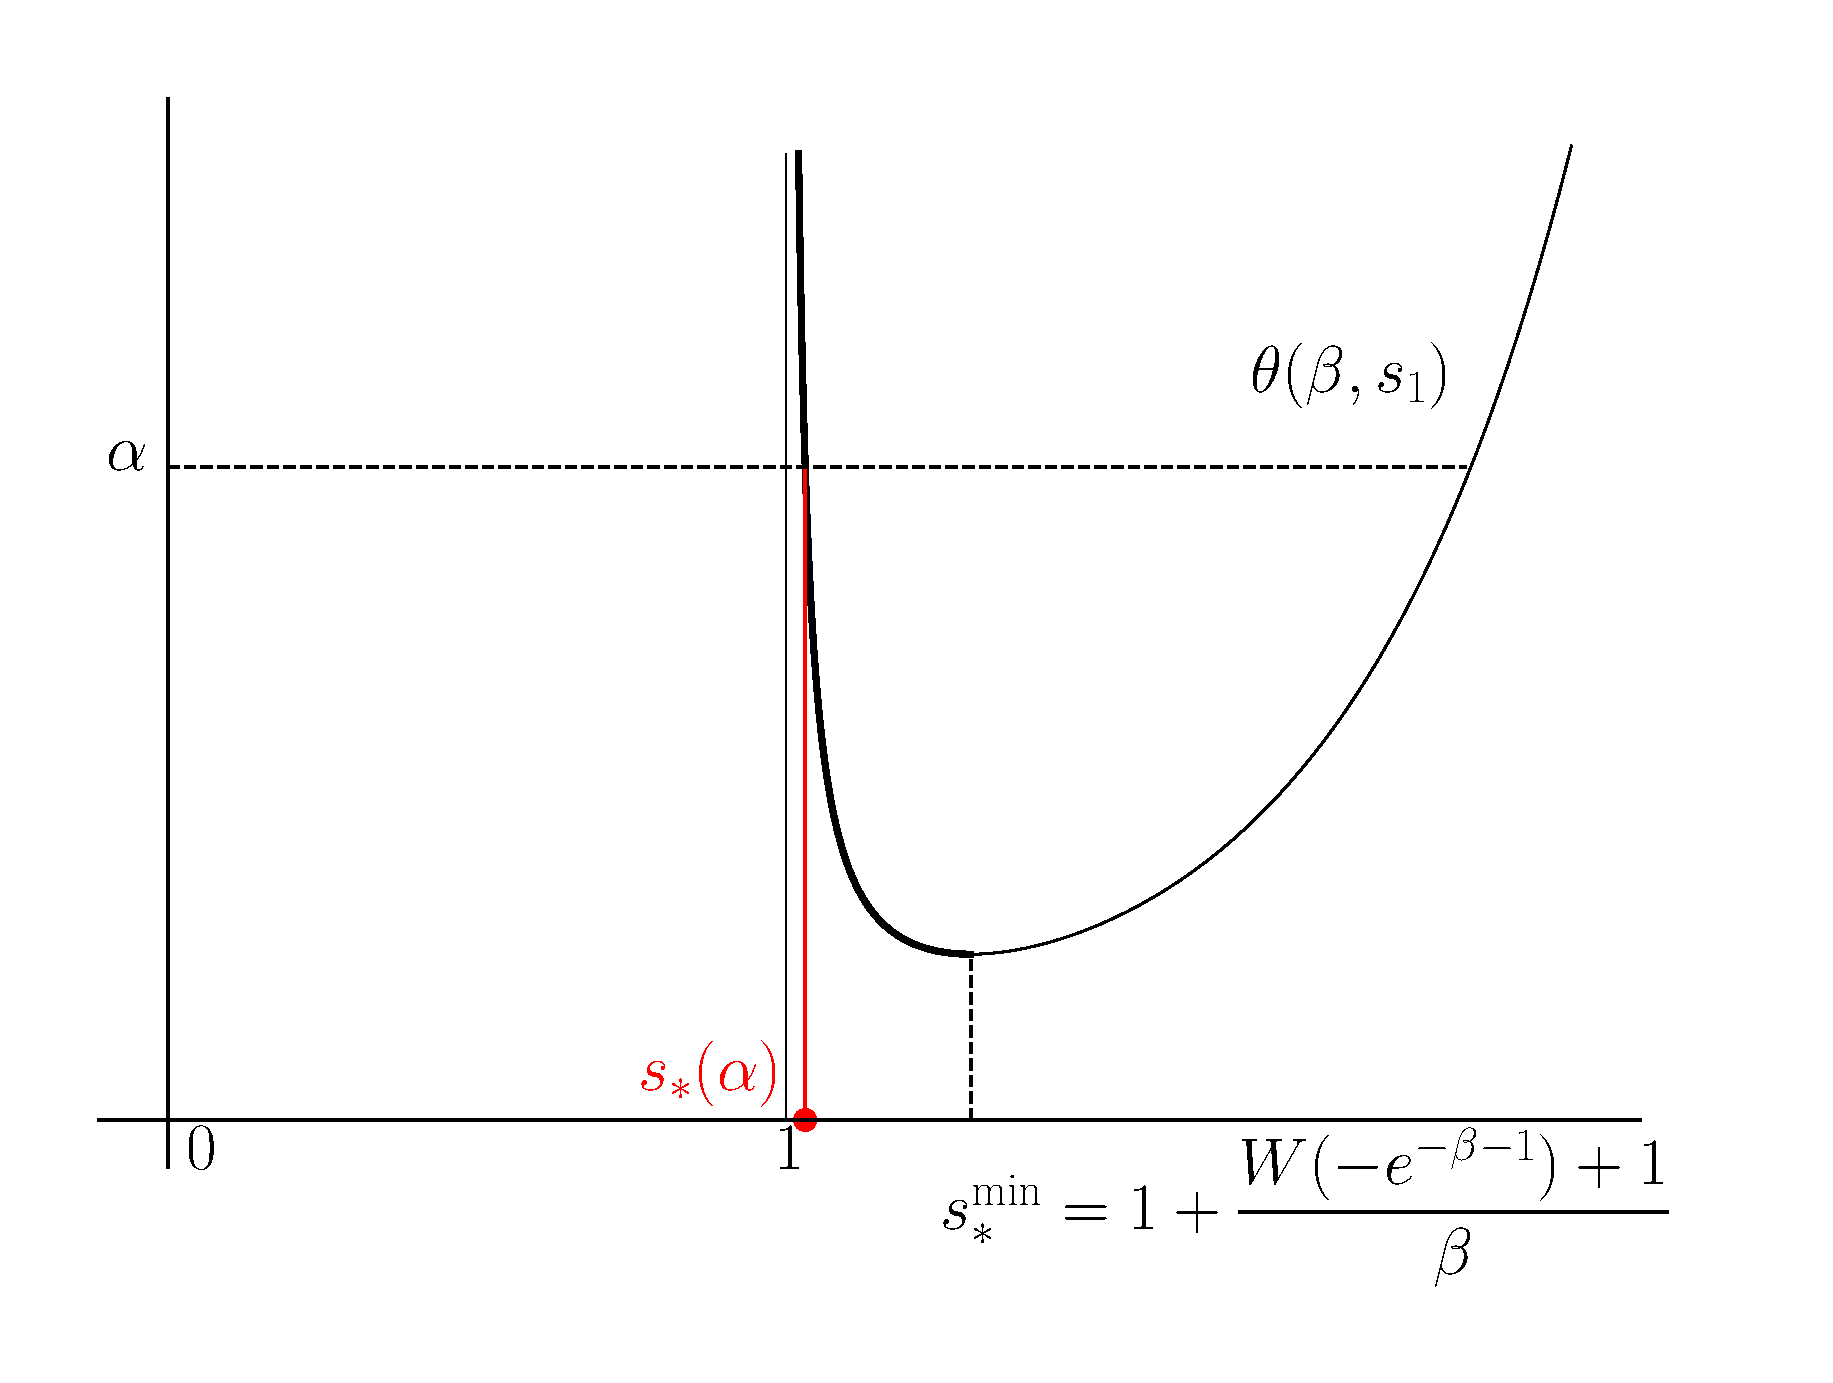
\includegraphics[width=0.7\textwidth]{theta.eps}
	\caption{При фиксированном $\beta$ функция $\theta(\beta,  s_*)$ имеет одну точку минимума $ s_*^{\min}$ и два промежутка монотонности $(1; + s_*^{\min}]$ и $[ s_*^{\min}; +\infty)$. Значение $ s_*(\alpha)$ определяется как меньший корень уравнения $\alpha = \theta(\beta,  s_*)$, поэтому левая ветвь (выделена толстой линией) определяет зависимость $ s_*(\alpha)$.}
\end{figure}


%
\begin{proposition}
	Правая часть уравнения \eqref{eq:period_eq_exp} стремится к $+\infty$ при $\alpha \to +\infty$.
\end{proposition}
\begin{proof}
	Заменим в правой части уравнения \eqref{eq:period_eq_exp} $\alpha = \dfrac{e^{\beta s_*} - 1}{e^{\beta}(s_* - 1)}$:
	\begin{equation}
		\dfrac{\alpha^2}{2}e^{\beta}( s_* - 1)^2 + \alpha s_* = \dfrac{1}{2}e^{-\beta}(e^{\beta s_*} - 1)^2 + \dfrac{s_*}{s_* - 1}\dfrac{e^{\beta s_*} - 1}{e^{\beta}}.
	\end{equation}
	Устремим $\alpha \to +\infty$, тогда $s_* \to 1 + 0$ и выражение стремится к $+\infty$ за счёт множителя $\dfrac{s_*}{s_* - 1} > 0$.
\end{proof}

Получаем, что левая часть уравнения \eqref{eq:period_eq_exp} от $\alpha$ не зависит, а правая принимает сколь угодно большие значения при больших $\alpha$.

В свою очередь, правая часть не зависит от $\Delta$, а левая эквивалентна $e^{\beta\Delta}$ при $\Delta \to +\infty$:
$$
\dfrac{1}{A(\Delta)}\left(e^{\beta\Delta(m + 1)} - 1\right) = \dfrac{e^{\beta\Delta(m + 1)} - 1}{e^{\beta} - 1 + \frac{e^{\beta\Delta(m + 1)} - 1}{e^{\beta\Delta} - 1}} \sim e^{\beta \Delta}.
$$

Таким образом, при фиксированных $\alpha$ и $\beta$ мы можем добиться равенства в уравнении \eqref{eq:period_eq_exp} за счёт увеличения $\Delta$; для этого нам нужно, чтобы левая часть уравнения была меньше правой для некоторого $\Delta$.

Фиксируем параметр $\beta > 0$.

Рассмотрим условие \eqref{eq:cond_th_w>1_t_1+1}. Произведём замену $\alpha = \dfrac{e^{\beta s_*} - 1}{e^{\beta}(s_* - 1)}$. Получим: 
\begin{equation}
	e^{-\beta  s_*} \left(e^{-\beta} + \frac{e^{\beta s_*} - 1}{e^{\beta}(s_* - 1)}s_*\right) > 1.
\end{equation}
%

\begin{proposition}
	Функция 
	\begin{equation}
		h(s_*) = e^{-\beta  s_*} \left(e^{-\beta} + \frac{e^{\beta s_*} - 1}{e^{\beta}(s_* - 1)}s_*\right)
	\end{equation}
	убывает при $s_* \geqslant 1$.
\end{proposition}
%
\begin{proof}
	\begin{equation}
		\dfrac{d}{ds_*}h(s_*) = -\dfrac{e^{-\beta(s_* + 1)} (e^{\beta s_*} - \beta s_* - 1 + \beta)}{(s_* - 1)^2}.
	\end{equation}
	% Из разложения экспоненты
	Поскольку $e^{\beta s_*} > 1 + \beta s_*$, получаем, что $\dfrac{d}{ds_*}h(s_*) < 0$, следовательно, $h$ убывает.
\end{proof}

Это значит, что если значение $s_* =  s_*^0 > 1$ удовлетворяет условию \eqref{eq:cond_th_w>1_t_1+1}, то значения $1 \leqslant  s_* \leqslant s_*^0$ также ему удовлетворяют.

Пусть $s_* = 1 + \dfrac{1}{e^{\beta}}$, тогда
\begin{equation}
	\alpha = \frac{e^{\beta s_*} - 1}{e^{\beta}(s_* - 1)} = e^{\beta(1 + e^{-\beta})} - 1.
\end{equation}

Убедимся, что выполнено условие \eqref{eq:cond_th_w>1_t_1+1}:
\begin{multline}
	e^{-\beta s_*}(e^{-\beta} + \alpha s_*) =
	e^{-\beta (1 + e^{-\beta})}\left(e^{-\beta} + (1 + e^{-\beta})(e^{\beta(1 + e^{-\beta})} - 1)\right) =\\
	= e^{-\beta (1 + e^{-\beta})} e^{-\beta} + (1 + e^{-\beta}) - (1 + e^{-\beta})e^{-\beta (1 + e^{-\beta})} = 1 + e^{-\beta} - e^{-\beta (1 + e^{-\beta})} > 1.
\end{multline}

Поскольку при увеличении $\alpha$ значение $s_*$ убывает, условие \eqref{eq:cond_th_w>1_t_1+1} будет выполнено при всех $\alpha \geqslant e^{\beta(1 + e^{-\beta})} - 1$.

Теперь нужно проверить выполнение условий Леммы \ref{lm:t1_locate}, которые соответствуют условиям \eqref{eq:cond_thm1} и \eqref{eq:cond_thm2} теоремы \ref{thm:mg_auxiliary_main}.

\begin{proposition}
	\label{prop:alpha_greater_phi}
	Если $\alpha > e^{\beta(1 + e^{-\beta})} - 1$, то $\alpha > \varphi(\beta)$.
\end{proposition}
\begin{proof}
	Согласно утверждению \ref{prop:phi_theta}, $\theta(\beta, \tau_*) \geqslant \varphi(\beta)$ независимо от выбора $\tau_*$. Положим $\tau_* = 2$ и докажем, что $e^{\beta(1 + e^{-\beta})} - 1 > \theta(\beta, 2)$.
	%
	\[
	e^{\beta(1 + e^{-\beta})} - 1 >
	e^{\beta} (1 + \beta e^{-\beta}) - 1 =
	e^{\beta} + \beta - 1 > e^{\beta} + e^{-\beta} = \theta(\beta, 2).
	\]
\end{proof}

Зафиксируем $\alpha, \beta$ и положим $\Delta =  s_*(\alpha)$. Тогда условие $\alpha \geqslant \theta(\beta, \Delta)$ выполнено (поскольку обращается в равенство).

\begin{proposition}
	При $s_* = \Delta < 1 + \frac{1}{e^{\beta}}$ верно неравенство
	$$
	\dfrac{1}{A(\Delta)}\left(e^{\beta\Delta(m + 1)} - 1\right) \leqslant \dfrac{\alpha^2}{2}e^{\beta}(s_* - 1)^2 + \alpha s_*.
	$$
\end{proposition}
\begin{proof}
	Оценим левую часть:
	\[
	\dfrac{1}{A(\Delta)}\left(e^{\beta\Delta(m + 1)} - 1\right) = \dfrac{e^{\beta\Delta(m + 1)} - 1}{e^{\beta} - 1 + \frac{e^{\beta\Delta(m + 1)} - 1}{e^{\beta\Delta} - 1}} < e^{\beta \Delta} - 1.
	\]
	%
	Докажем, что правая часть больше $e^{\beta \Delta} - 1$:
	\begin{multline*}
		\dfrac{\alpha^2}{2}e^{\beta}(\Delta - 1)^2 + \alpha\Delta = \dfrac{1}{2}e^{-\beta}(e^{\beta\Delta} - 1)^2 + \dfrac{\Delta}{\Delta - 1}\dfrac{e^{\beta\Delta} - 1}{e^{\beta}} > e^{\beta \Delta} - 1 \Leftrightarrow\\
		\dfrac{1}{2}(e^{\beta\Delta} - 1) + \dfrac{\Delta}{\Delta - 1} > e^{\beta} \Leftrightarrow
		\dfrac{1}{2}(e^{\beta\Delta} - 1) + 1 + \dfrac{1}{\Delta - 1} > e^{\beta}.
	\end{multline*}
	Поскольку $1 < \Delta < 1 + \frac{1}{e^{\beta}}$,
	$$
	\dfrac{1}{2}(e^{\beta\Delta} - 1) + 1 + \dfrac{1}{\Delta - 1} \geqslant \dfrac{1}{2}(e^{\beta\Delta} - 1) + 1 + e^{\beta} > e^{\beta},
	$$
	что и требовалось.
\end{proof}

% Вроде бы эта лемма следует из того, что gamma определяется как левый корень уравнения, а он левее точки минимума.
\begin{lemma}
	\label{lm:delta_min}
	$$\dfrac{W(-e^{-\beta - 1}) + 1}{\beta} > \dfrac{1}{e^{\beta}}.$$
\end{lemma}
\begin{proof}
	\begin{multline*}
		\dfrac{W(-e^{-\beta - 1}) + 1}{\beta} > \dfrac{1}{e^{\beta}} \Leftrightarrow
		W(-e^{-\beta - 1}) > \beta e^{-\beta} - 1 \Leftrightarrow \\
		-e^{-\beta - 1} > (\beta e^{-\beta} - 1)\exp(\beta e^{-\beta} - 1) \Leftrightarrow \\
		\exp(-\beta - \beta e^{-\beta}) < 
		1 - \beta e^{-\beta} \Leftrightarrow \exp(-\beta(1 + e^{-\beta})) < 1 - \beta e^{-\beta}.
	\end{multline*}
	Поскольку $\exp(-\beta(1 + e^{-\beta})) < e^{-\beta}$, докажем, что $e^{-\beta} < 1 - \beta e^{-\beta}$:
	\[
	e^{-\beta} < 1 - \beta e^{-\beta} \Leftrightarrow e^{\beta} > 1 + \beta,
	\]
	что верно при любом $\beta > 0$.
\end{proof}

Функция $\theta(\beta, \Delta)$ убывает на промежутке $(1; \Delta_{\text{min}}]$, где (см. утверждение \ref{prop:phi_theta})
%
\[\Delta_{\text{min}} = 1 + \dfrac{W(-e^{-\beta - 1}) + 1}{\beta} > 1 + \dfrac{1}{e^{\beta}}\]
%
по лемме \ref{lm:delta_min}, значит, условие $\alpha > \theta(\beta; \Delta)$ на нём также будет выполнено. %% на самом деле, при delta > 2 ограничение на theta стабилизируется, но так даже лучше, поэтому пофигу.

При $\Delta > \Delta_{\text{min}}$ уже требуется выполнение условия $\alpha \geqslant \varphi(\beta)$, а оно выполняется согласно утверждению \ref{prop:alpha_greater_phi}.

Таким образом, условия леммы 
\ref{lm:t1_locate} остаются верны при увеличении $\Delta$. Значит, найдётся $\Delta$, удовлетворяющее уравнению \eqref{eq:period_eq_exp}.

Докажем, что при определённых таким образом параметрах $\alpha, \beta, \Delta$ выполнены условия леммы \ref{lm:lem_w>1}, которые соответствуют условиям (\ref{eq:cond_hair_hair_01} -- \ref{eq:cond_hair_hair_1}) теоремы \ref{thm:mg_auxiliary_main}. По построению $s_* < \tau_k - \tau_{k - 1} = \Delta$, поэтому при $k \geqslant 2$ мы должны проверять набор условий \eqref{eq:cond_hair_hair_01}:
\[
\frac{\alpha^2}{2}e^\beta(s_*-1)^2+\alpha s_* > \frac{e^{\beta \tau_k}-1}{\sum_{i=0}^{k-1}e^{\beta \tau_i}},\quad k=1,\ldots,m.
\]
%
Перепишем правую часть с учётом $\Delta > 1$.
\[
\frac{e^{\beta \tau_k}-1}{\sum_{i=0}^{k-1}e^{\beta \tau_i}} = \frac{e^{\beta\Delta k } - 1}{e^{\beta} - 1 + \frac{e^{\beta\Delta k} - 1}{e^{\beta\Delta} - 1}} = \frac{1}{\frac{e^{\beta} - 1}{e^{\beta\Delta k} - 1} + \frac{1}{e^{\beta\Delta} - 1}}.
\]
%
Заметим, что это выражение возрастает по $k$, поэтому достаточно выполнение условия при $k = m$. Но при подстановке $k = m + 1$ мы получаем равенство \eqref{eq:period_eq_exp}, поэтому при $k \leqslant m$ оно обратится в нужное нам неравенство.

При $k = 1$ и $s_* > \tau_1 - \tau_0 = \Delta - 1$ нужно проверять условие \eqref{eq:cond_hair_hair_02}. Докажем, что оно слабее условия \eqref{eq:cond_th_w>1_t_1+1}, которое было проверено ранее. Запишем условие \eqref{eq:cond_hair_hair_02} при $k=1$:
\[
\frac{\alpha^2}{2} e^{\beta}(s_* - 1)^2 + \alpha s_* > \frac{e^{\beta (s_* + 1)} - 1}{e^{\beta}} \Leftrightarrow \left(\frac{\alpha^2}{2} e^{\beta}(s_* - 1)^2 + \alpha s_* + e^{-\beta}\right)e^{-\beta s_*} > 1.
\]
%
Но нам известно, что из условия \eqref{eq:cond_th_w>1_t_1+1},
\[
\left(\alpha s_* + e^{-\beta}\right)e^{-\beta s_*} > 1,
\]
%
а положительная добавка
\[\dfrac{\alpha^2}{2} e^{\beta}(s_* - 1)^2 e^{-\beta s_*}\]
делает неравенство ещё строже.

% На самом деле так не бывает, \Delta < 2.
Если же $s_* \leqslant \Delta - 1$, то для случая $k = 1$ верны те же рассуждения, что и для случая $2 \leqslant k \leqslant m$.

Для выполнения условий \eqref{eq:cond_hair_hair_1}:
\[
\frac{\alpha^2}{2}e^\beta(-1)^2+\alpha s_*>\frac{e^{\beta \tau_k}(e^{\beta s_*}-\alpha s_*)-1}{\sum_{i=0}^{k-1}e^{\beta \tau_i}},\quad k = 1,\ldots, m
\]
достаточно проверить, что верно неравенство
\[
e^{\beta s_*}-\alpha s_* \leqslant 1,
\]
тогда они окажутся слабее уже доказанного набора условий \eqref{eq:cond_hair_hair_01}. Замечание: мы действительно доказали их справедливость при всех $1 \leqslant k \leqslant m$, но при $k = 1$, возможно, проверяется условие из набора \eqref{eq:cond_hair_hair_02}.

Выполним замену $e^{\beta s_*} - 1 = \alpha e^\beta (s_* - 1)$.
%
\[
\alpha e^{\beta}(s_* - 1) - \alpha s_* \leqslant 0 \Leftrightarrow e^{\beta}(s_* - 1) - s_* \leqslant 0 \Leftrightarrow s_* \leqslant 1 + \frac{1}{e^{\beta} - 1}.
\]
%
По построению $s_* < 1 + \frac{1}{e^{\beta}}$, поэтому неравенство верно.
%
Из результатов, полученные в данном разделе, следует
%
\begin{theorem}
	\label{thm:relay_main}
	Для произвольных $\beta > 0$, $\alpha \geqslant e^{\beta\left(1 + \frac{1}{e^{\beta}}\right)} - 1$ найдётся $\Delta > 1$, при котором набор параметров $\alpha, \beta, \Delta$ удовлетворяет уравнению \eqref{eq:period_eq} и условиям (\ref{eq:cond_thm1} -- \ref{eq:cond_hair_hair_1}) теоремы \eqref{thm:mg_auxiliary_main}.
\end{theorem}


\section{Численные результаты}\label{sec:ch2/sect4}
%
На рисунках \ref{fig:solution_2d} и \ref{fig:solution_3d} приведены результаты численного эксперимента для систем \eqref{eq:system_relay} и \eqref{eq:mg_full_renormed}. Отметим, что при $\gamma=100$ графики решений систем \eqref{eq:system_relay} и \eqref{eq:mg_full_renormed} визуально не отличимы.

% Картинки 2022-04-30-численный-счёт.ipynb

\begin{figure}
	\centering
	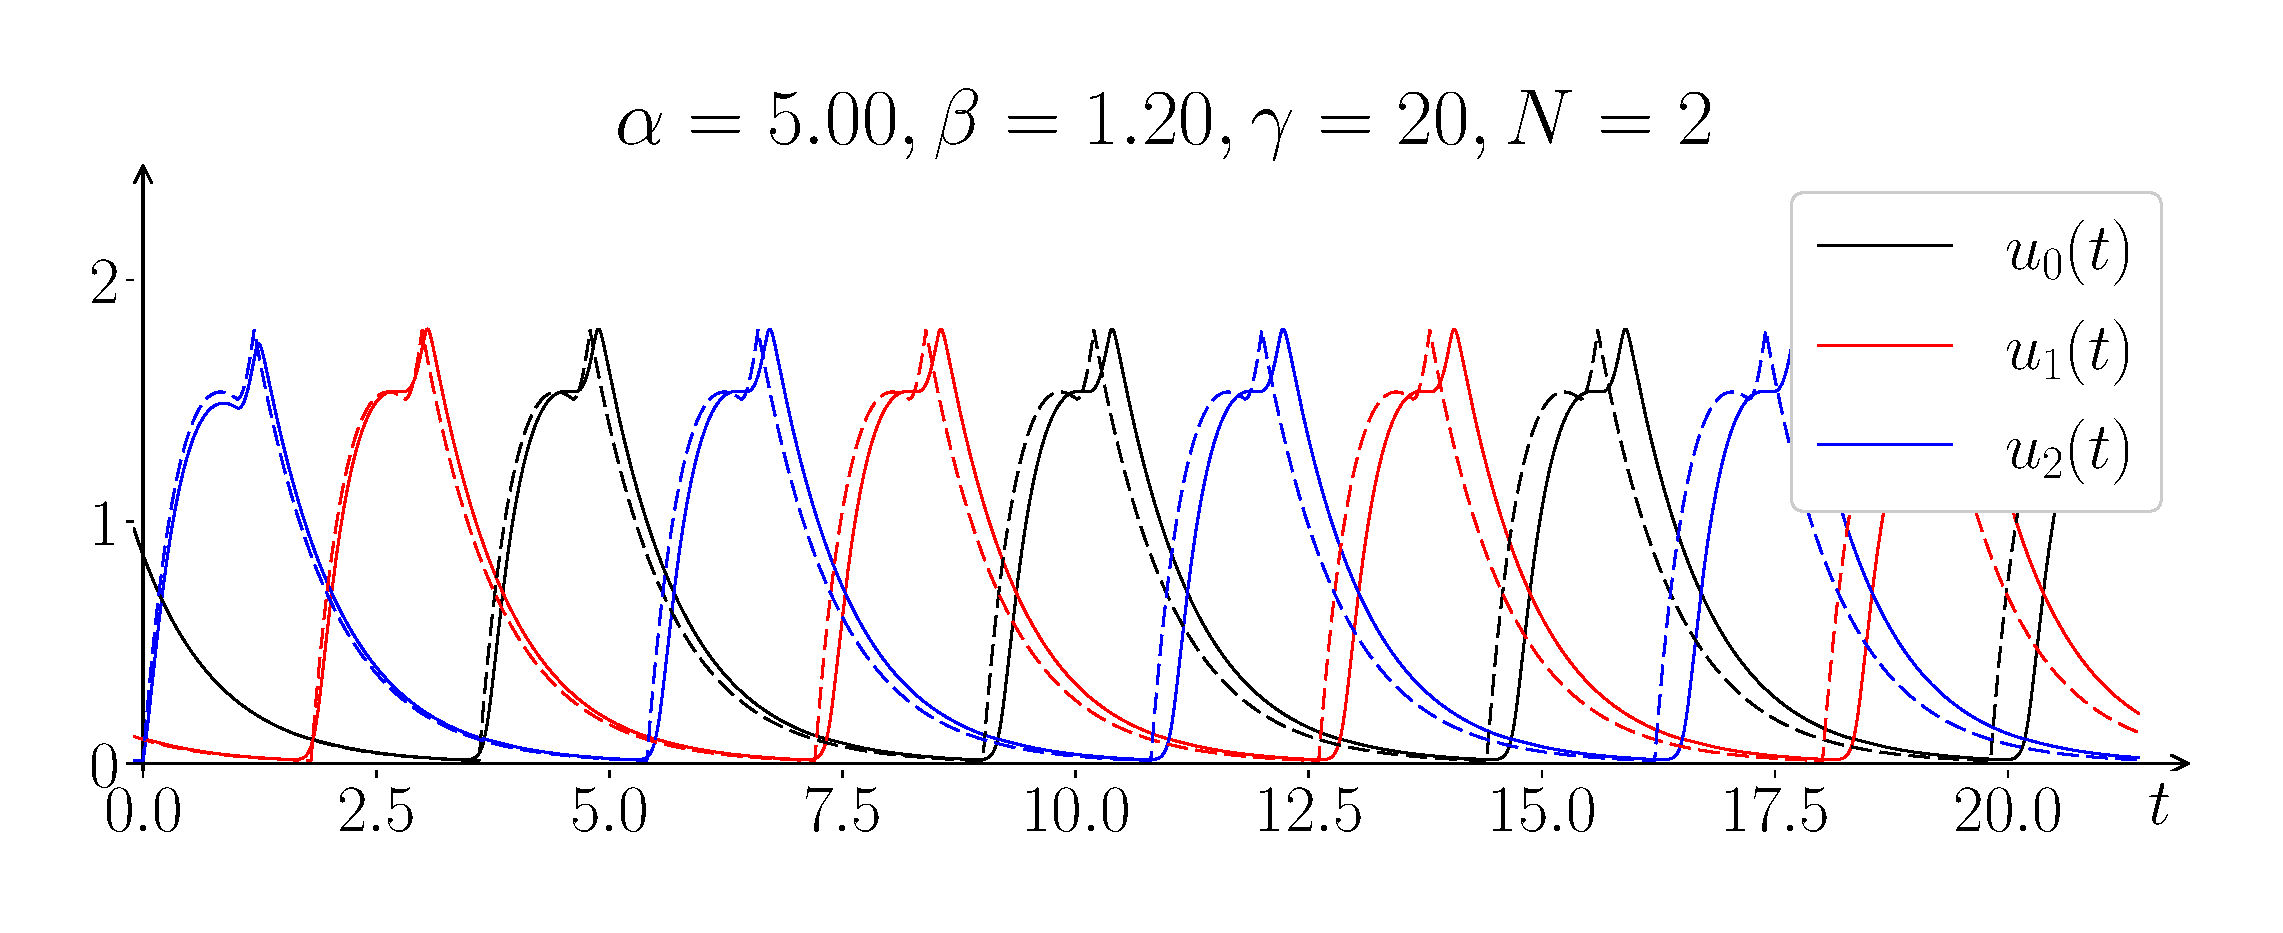
\includegraphics[width=\textwidth]{alpha_5_beta_1p2_multi.eps}
	\caption{Пунктирной линией изображено периодическое решение предельной системы  \eqref{eq:system_relay}, полученное численно для параметров $m = 2, \alpha = 5.0, \beta = 1.2, \Delta \approx 1.801$. Сплошная линия изображает решение системы \eqref{eq:mg_full_renormed} для значения показателя $\gamma = 10$.}
	\label{fig:solution_2d}
\end{figure}

\begin{figure}
	\centering
	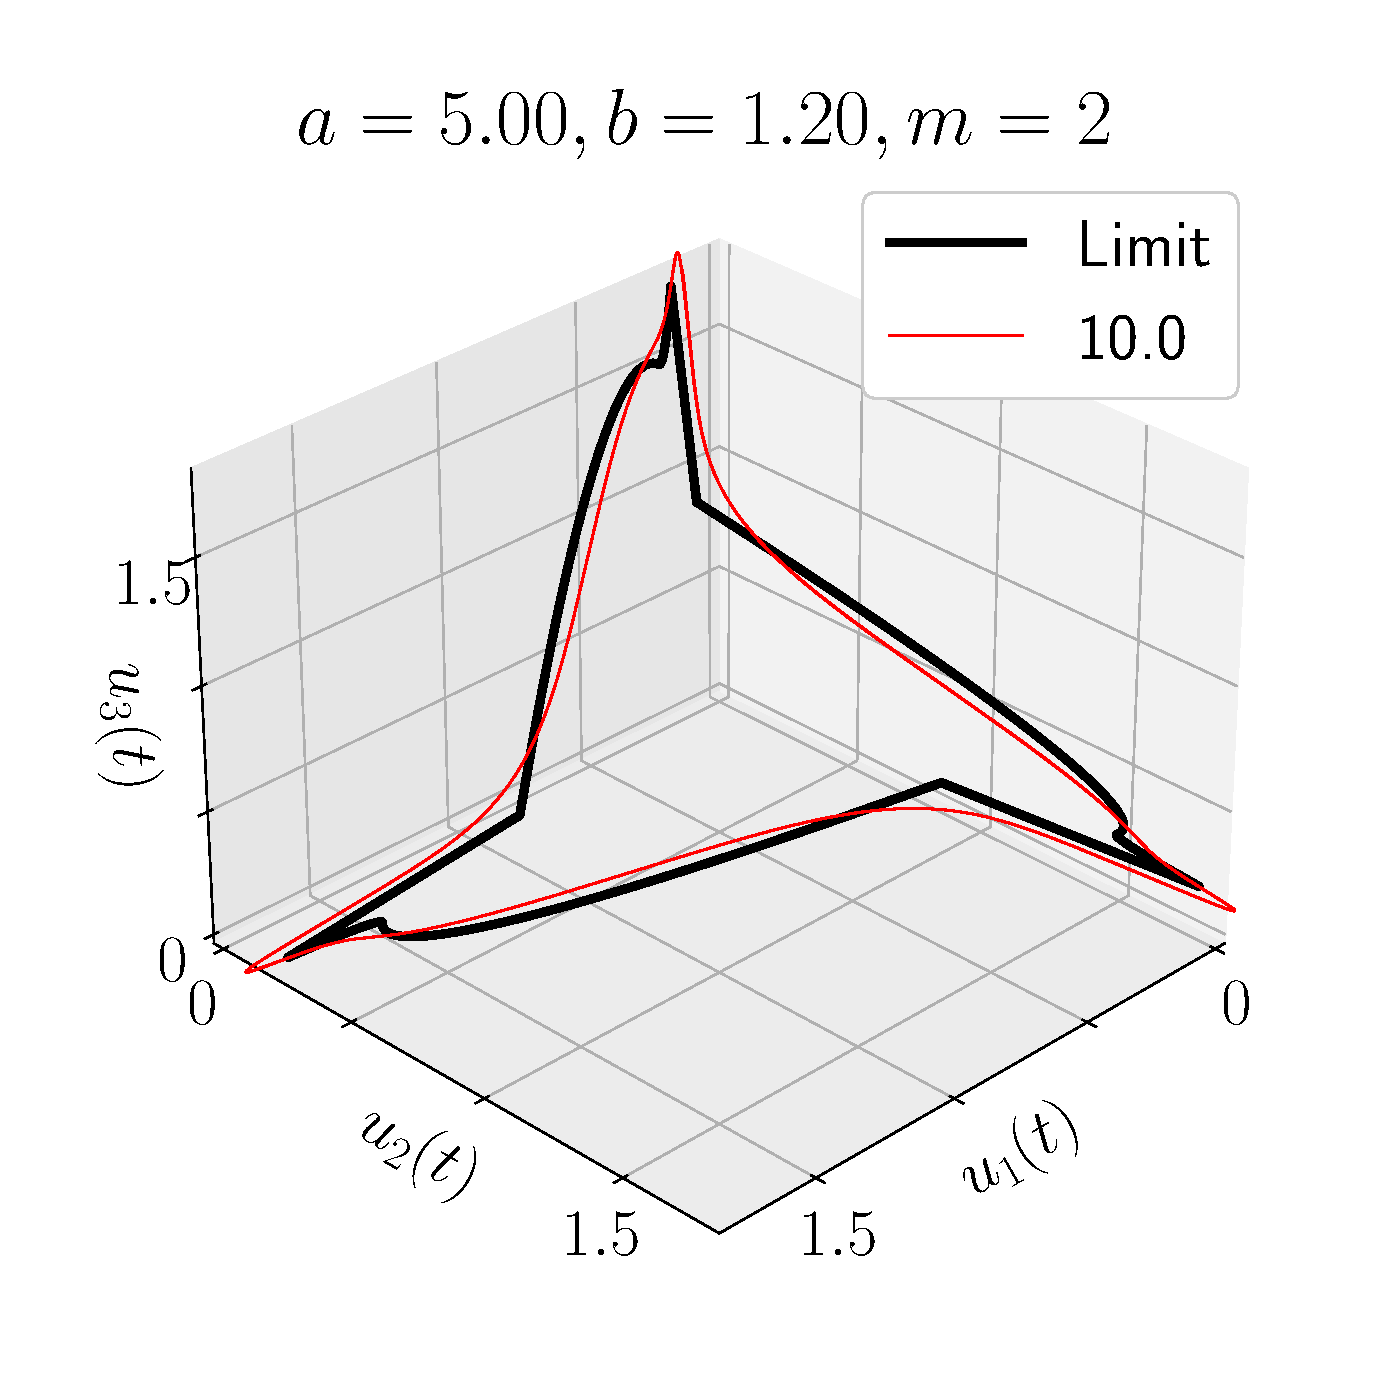
\includegraphics[width=0.48\textwidth]{alpha_5_beta_1p2_3d_10.eps}\hfill
	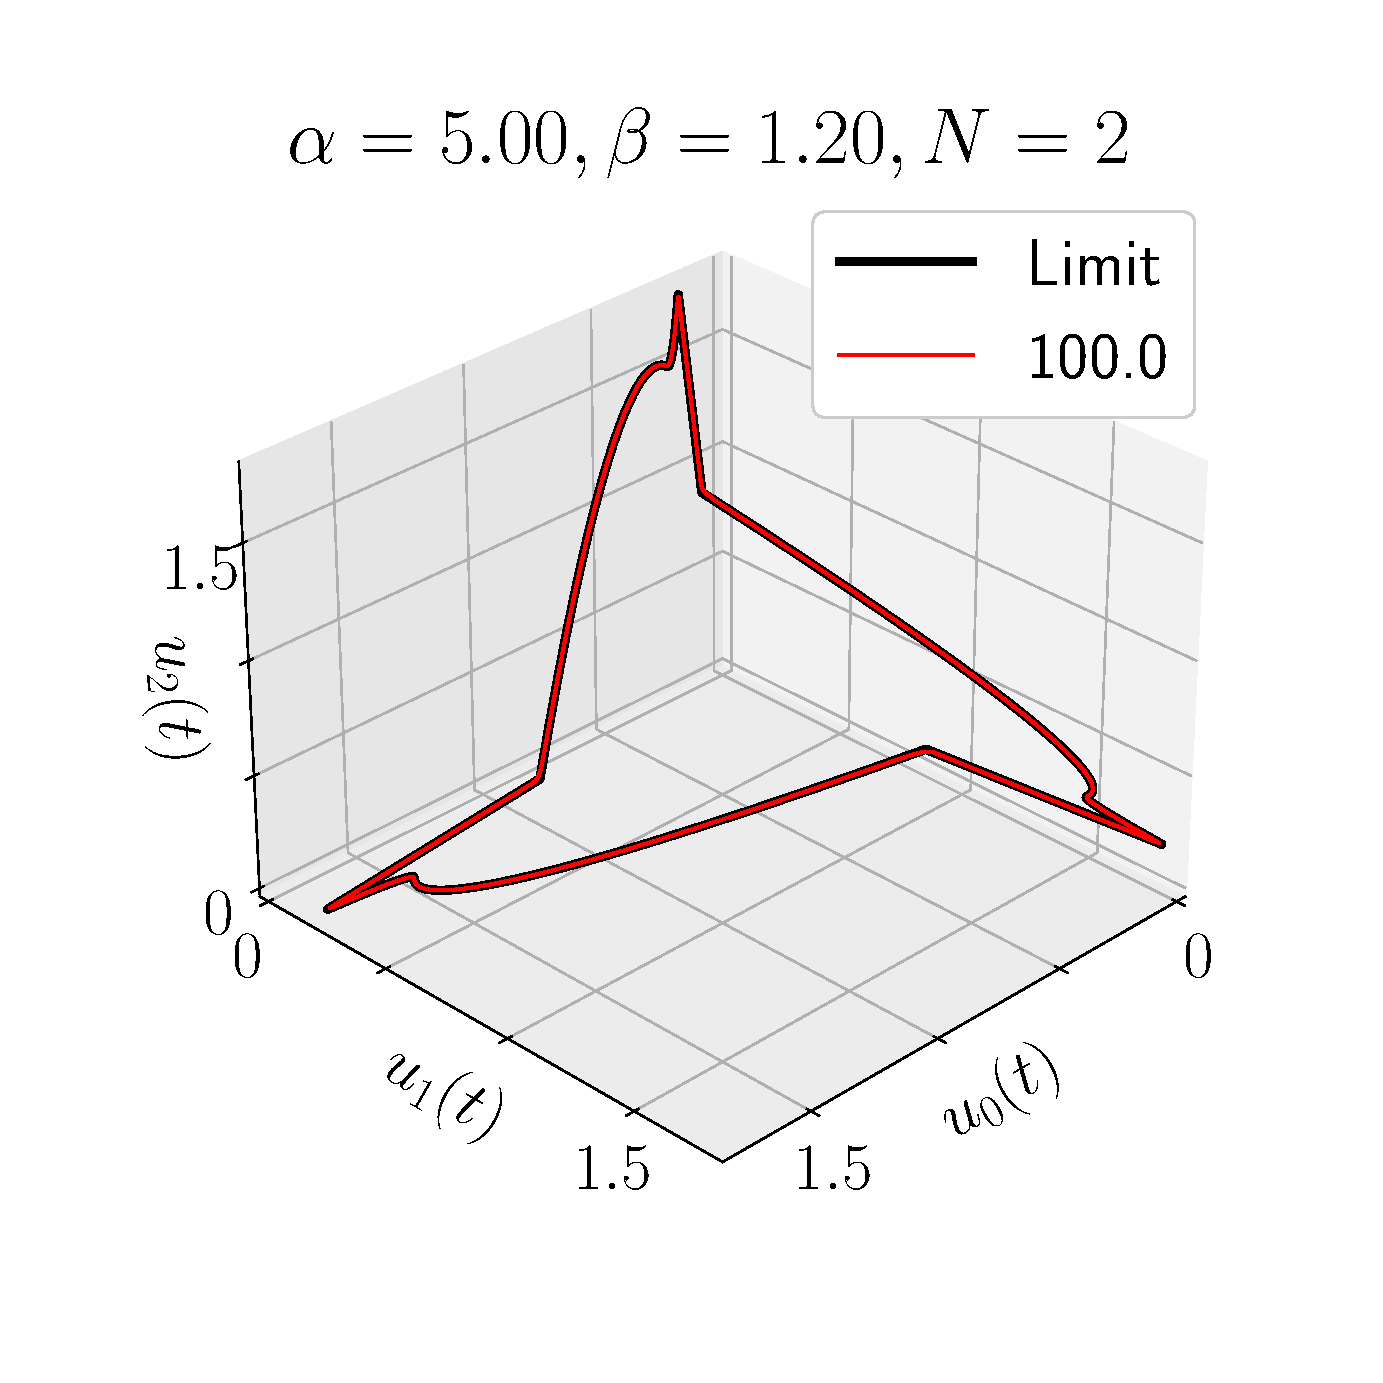
\includegraphics[width=0.48\textwidth]{alpha_5_beta_1p2_3d_100.eps}
	\caption{Иллюстрация периодического решения предельной системы \eqref{eq:system_relay} в псевдофазовом пространстве в сравнении с решением системы \eqref{eq:mg_full_renormed} при $\gamma = 10$ (слева) и $\gamma = 100$ (справа).}
	\label{fig:solution_3d}
\end{figure}

%TODO: взять статью из диффуров и скопировать оттуда ещё картинки

\section{Выводы к главе 2}\label{sec:ch2/sect5}

В данной главе проведено исследование предельного при $\gamma \to +\infty$ объекта для системы \eqref{eq:mg_full_renormed}, описывающей полносвязную систему генераторов Мэки--Гласса. Для релейной системы \eqref{eq:system_relay} показано (при некоторых ограничениях на параметры) существование периодического режима в виде <<дискретной бегущей волны>> -- режима, при котором компоненты решения отличаются друг от друга сдвигом (в некотором порядке) на фиксированную величину. Явное описание решения и ограничений на параметры дано в теореме \ref{thm:mg_auxiliary_main}. В теореме \ref{thm:relay_main} приведено семейство параметров с более простым аналитическим описанием.
           % Глава 2
\chapter{Режимы двухкластерной синхронизации в полносвязной цепи генераторов Мэки--Гласса}\label{ch:ch3}

Как и в главе \eqref{ch:ch2}, в текущей главе рассматривается генератор Мэки-Гласса --- электрический генератор, функция напряжения $V(t)$ которого описывается уравнением Мэки-Гласса
%
\begin{equation}
	\label{eq:mg:ch3}
	\dfrac{d V}{dt}=
	- bV+\dfrac{acV(t - \tau) }{1 + (cV(t - \tau))^{\gamma}}.
\end{equation}
%
Здесь $V=V(t) > 0$ --- скалярная функция, $a, b, c, \tau, \gamma$ --- положительные параметры. Параметр $\tau$ --- запаздывание по времени, параметр $\gamma$ определяет форму нелинейности.

Пусть в распоряжении имеется произвольное (фиксированное) число генераторов Мэки--Гласса \eqref{eq:mg:ch3}. Рассмотрим полносвязную цепь генераторов, где каждый генератор связан с каждым. В этом случае можно поставить вопрос поиска периодических режимов двухкластерной синхронизации --- таких решений, что все компоненты совпадают с одной из двух различных периодических функций.

В разделе \ref{sec:ch3/sect1} описывается система дифференциальных уравнений с запаздывающим аргументом, соответствующая режиму двухкластерной синхронизации. Производится переход к новым переменным. В разделе \ref{sec:ch3/sect2} доказывается обратимость проведённой замены. В разделе \ref{sec:ch3/sect3} для предельной при $\gamma \to +\infty$ системы отыскивается решение, которое при $t \to +\infty$ стремится к периодическому. В разделе \ref{sec:ch3/sect4} доказывается существование периодического режима двухкластерной синхронизации. В разделе \ref{sec:ch3/sect5} приводятся результаты численного моделирования.

%%%%%%%%%%%%%%%%%%%%%%%%%%%%%%%%%%%%%%%%%%%
\section{Постановка задачи}\label{sec:ch3/sect1}
%%%%%%%%%%%%%%%%%%%%%%%%%%%%%%%%%%%%%%%%%%%
Зафиксируем натуральные $m$ и $n$. Рассмотрим полносвязную цепь из $N = m + n$ генераторов Мэки-Гласса, т.~е. цепь, в которой каждый генератор взаимодействует со всеми остальными. Такая цепь задаётся системой
%
\begin{equation}
	\label{eq:mg_system}
	\dfrac{d V_{j}}{dt}= -bV_{j} + \dfrac{ac\left(V_{j}(t - \tau) + \delta\sum_{k=1,k\neq j}^{N}V_{k}(t)\right)}{1 + \left(c\left(V_{j}(t - \tau) + \delta\sum_{k=1,k\neq j}^{N}V_{k}(t)\right)\right)^{\gamma}}, \quad j=1, 2, \ldots, N,
\end{equation}
где $V_j(t) > 0$ для всех $j = 1, \ldots, N$, коэффициент $\delta > 1$ контролирует силу связи. 

После замен $V_j = c^{-1}u_j(\frac{t}{\tau})$, $\beta = b\tau$, $\alpha=ac\tau$, $t \mapsto \frac{t}{\tau}$,
перейдём от системы (\ref{eq:mg_system}) к более удобной форме с меньшим числом параметров:
%
\begin{equation}
	\label{eq:mg_system_norm}
	\dot{u}_j=-\beta u_j+\frac{\alpha\big(u_j(t - 1) + \delta\sum_{k = 1, k\neq j}^{N}u_{k}(t)\big)}{1+\big(u_j(t - 1) + \delta\sum_{k = 1, k \neq j}^{N}u_{k}(t)\big)^\gamma}, \quad j = 1, 2, \ldots, N.
\end{equation}
%
Здесь $\alpha, \beta > 0$, $u_j(t) > 0$ для всех $j = 1, \ldots, N$.

Пусть
%
\begin{equation}
	\label{eq:F_func}
	F(x) = \dfrac{x}{1 + x^\gamma}.
\end{equation}

С учётом \eqref{eq:F_func} система \eqref{eq:mg_system_norm} примет вид:
%
\begin{equation}
	\label{eq:mg_system_norm_F}
	\dot{u_j} = -\beta u_j + \alpha\,F\left(u_j(t - 1) + \delta \sum_{k = 1, k\neq j}^{N}u_{k}(t)\right), \quad j = 1, \ldots, N.
\end{equation}

Будем искать режимы двухкластерной синхронизации, т.~е. периодические режимы, в которых $m$ генераторов описываются функцией $u(t)$, а остальные $n$ генераторов --- другой функцией $v(t)$.

Система \eqref{eq:mg_system_norm_F} примет вид:
%
\begin{equation}
	\label{eq:mg_cluster_system_norm}
	\begin{cases}
		\dot{u} = -\beta u + \alpha \, F \big(u(t - 1) + \delta (m - 1) u + \delta n v\big),\\
		\dot{v} = -\beta v + \alpha  \, F \big(v(t - 1) + \delta m u + \delta (n - 1) v\big).
	\end{cases}
\end{equation}

После замен
\begin{equation}
	\label{eq:tilde_change}
	\tilde{u}(t) = u(t - 1) + \delta (m - 1) u + \delta n v, \quad \tilde{v}(t) = v(t - 1) + \delta m u + \delta (n - 1) v,
\end{equation}

система \eqref{eq:mg_cluster_system_norm} примет вид
%
\begin{equation}
	\label{eq:mg_cluster_system_pre_tilde}
	\begin{cases}
		\dot{u} = -\beta u + \alpha \, F(\tilde{u}),\\
		\dot{v} = -\beta v + \alpha \, F(\tilde{v}).
	\end{cases}
\end{equation}


Перепишем систему \eqref{eq:mg_cluster_system_pre_tilde} через переменные $\tilde{u}$ и $\tilde{v}$.
\begin{multline*}
	\dot{\tilde{u}}(t) = \dot{u}(t - 1) + \delta (m - 1) \dot{u} + \delta n \dot{v} =\\= \left(-\beta u(t - 1) + \alpha \, F(\tilde{u}(t - 1))\right) + \delta (m - 1)(-\beta u + \alpha\, F(\tilde{u})) + \delta n (-\beta v + \alpha \, F(\tilde{v})) =\\
	= -\beta(u(t - 1) + \delta (m - 1)u + \delta nv) + \alpha\big(F(\tilde{u}(t - 1)) + \delta (m - 1) \, F(\tilde{u}) + \delta n \, F(\tilde{v})\big) = \\
	= -\beta \tilde{u} + \alpha \big(F(\tilde{u}(t - 1)) + \delta (m - 1)\, F(\tilde{u}) + \delta n \, F(\tilde{v})\big).
\end{multline*}

Аналогично,
\[
\dot{\tilde{v}} = -\beta \tilde{v} + \alpha \big(F(\tilde{v}(t - 1)) + \delta m \, F(\tilde{u}) + \delta (n - 1) \, F(\tilde{v})\big).
\]

Получаем систему:
%
\begin{equation}
	\label{eq:mg_cluster_system_tilde}
	\begin{cases}
		\dot{\tilde{u}} = -\beta \tilde{u} + \alpha \big(F(\tilde{u}(t - 1)) + \delta (m - 1) \, F(\tilde{u}) + \delta n \, F(\tilde{v})\big),\\
		\dot{\tilde{v}} = -\beta \tilde{v} + \alpha \big(F(\tilde{v}(t - 1)) + \delta m \, F(\tilde{u}) + \delta (n - 1) \, F(\tilde{v})\big).
	\end{cases}
\end{equation}
% По ходу возник вопрос, почему функции u~ и v~ будут дифференцируемы (в смысле не будет точек, в которых производные справа и слева отличаются, как это бывает в методе шагов). Ответ простой: если в какой-то точке производные бы отличались слева и справа, то правая часть отличалась бы слева и справа, но она непрерывная. Значит, всё ок. Более того, решение непрерывно дифференцируемое, т.к. производные равны непрерывным функциям в правой части.

Поскольку $\tilde{u} > 0$, $\tilde{v} > 0$, можно провести экспоненциальные замены
\begin{equation}
	\label{eq:exp_change}
	\tilde{u} = e^x, \quad \tilde{v} = e^y.
\end{equation}

Вводя новую функцию $G(x) = e^{-x} \, F(e^x)$, получаем итоговый вид системы:
\begin{equation}
	\label{eq:system_main}
	\begin{cases}
		\dot{x} = -\beta + \alpha \left(e^{x(t - 1) - x} G(x(t - 1)) + \delta (m - 1) G(x) + \delta n e^{y - x} G(y)\right),\\
		\dot{y} = -\beta + \alpha \left(e^{y(t - 1) - y} G(y(t - 1)) + \delta m e^{x - y} G(x) + \delta (n - 1) G(y)\right).
	\end{cases}
\end{equation}

\section{Обратимость замены}\label{sec:ch3/sect2}

Докажем, что решение $(u, v)$ системы \eqref{eq:mg_cluster_system_norm} однозначно восстанавливается по решению $(x, y)$ системы \eqref{eq:system_main}.

% Здесь нужна дифференцируемость, а не только непрерывность, т.к. дальше в операторе A у нас присутствует производная функции u. Но просто дифференцируемости недостаточно, т.к. пространство дифф. функций не полно, поэтому потребуем непрерывную дифференцируемость. u~, v~ непрерывно дифференцируемы (см. замечание выше), так что всё корректно.
\begin{lemma}
	\label{lm:uv_from_tilde}
	Пусть $\tilde{u}(t), \tilde{v}(t)$ --- $T$-периодические ($T > 0$) непрерывно дифференцируемые функции. Тогда существуют и определены единственным образом непрерывно дифференцируемые $T$-периодические функции $u(t), v(t)$, удовлетворяющие соотношениям \eqref{eq:tilde_change}.
\end{lemma}
\begin{proof}
	Перепишем систему \eqref{eq:tilde_change} в матричной форме:
	\[
	\begin{pmatrix}
		\tilde{u}\\
		\tilde{v}
	\end{pmatrix} = 
	\begin{pmatrix}
		u(t - 1)\\
		v(t - 1)
	\end{pmatrix} +
	\delta \cdot
	\begin{pmatrix}
		m - 1 & n \\
		m & n - 1
	\end{pmatrix}
	\begin{pmatrix}
		u\\
		v
	\end{pmatrix}.
	\]
	
	Обозначим
	\[
	J = 
	\delta \cdot
	\begin{pmatrix}
		m - 1 & n \\
		m & n - 1
	\end{pmatrix}, \quad
	\varphi =
	\begin{pmatrix}
		u\\
		v
	\end{pmatrix}, \quad
	\tilde{\varphi} =
	\begin{pmatrix}
		\tilde{u}\\
		\tilde{v}
	\end{pmatrix}
	\]
	
	Выразим $\varphi$:
	\begin{equation}
		\label{eq:tilde_matrix_form}
		\varphi = 
		J^{-1}
		\left(
		\tilde{\varphi} -
		\varphi(t - 1)
		\right),
		\text{ где }
		J^{-1} = \dfrac{1}{\delta(m + n - 1)} 
		\begin{pmatrix}
			1 - n & n \\
			m & 1 - m
		\end{pmatrix}.
	\end{equation}
	
	Пусть $(C^1[0, T])^2$ --- пространство пар непрерывно дифференцируемых $T$-периодических функций $\mathbb{R} \to \mathbb{R}$ с нормой
	
	\[\Vert (f, g) \Vert = \Vert f \Vert_{C^1} + \Vert g \Vert_{C^1} = \sup\limits_{[0, T]} |f| + \sup\limits_{[0, T]} |f'| + \sup\limits_{[0, T]} |g| + \sup\limits_{[0, T]} |g'|.\]
	
	Определим оператор $\mathcal{L}:(C^1[0, T])^2 \to (C^1[0, T])^2$:
	%\[\mathcal{L}: \varphi \mapsto \left(\psi: t \mapsto J^{-1} \left[ \tilde{\varphi} - \varphi(t - 1) \right] \right)\]
	\[\mathcal{L}\varphi = J^{-1} \left(\tilde{\varphi} - \varphi(t - 1) \right).\]
	
	Оператор $\mathcal{L}$ является сжимающим на $(C^1[0, T])^2$, т.к.
	\[\Vert\mathcal{L}\varphi - \mathcal{L}\psi\Vert = \Vert J^{-1} (\psi(t - 1) - \phi(t - 1)) \Vert \leq \Vert J^{-1} \Vert \cdot \Vert \psi - \phi \Vert = \dfrac{1}{\delta} \Vert \psi - \phi \Vert,\]
	%
	где $\Vert J^{-1} \Vert = \frac{1}{\delta} < 1$ --- 1-норма матрицы $J^{-1}$.
	
	Поскольку пространство $(C^1[0, T])^2$ полно, существует единственная неподвижная точка $\varphi_*$ оператора $\mathcal{L}$, которая удовлетворяет равенству \eqref{eq:tilde_matrix_form}.
\end{proof}

\begin{lemma}
	\label{lm:uv_inverse_system}
	Пусть $\tilde{u}, \tilde{v}$ --- $T$-периодические функции, являющиеся решением системы \eqref{eq:mg_cluster_system_tilde}. Тогда $T$-периодические функции $u, v$, однозначно выражаемые из соотношений \eqref{eq:tilde_change}, являются решением системы \eqref{eq:mg_cluster_system_norm}.
\end{lemma}
\begin{proof}
	Введём обозначение:
	\begin{equation}
		\label{eq:operator_A_definition}
		A_{m, n}(u, v) = -\beta u + \alpha \, F\big(u(t - 1) + \delta (m - 1)u + \delta n v \big) - \dot{u}.
	\end{equation}
	%
	Тогда система \eqref{eq:mg_cluster_system_norm} при фиксированных $m, n$ примет вид
	\begin{equation}
		\label{eq:uv_system_operator_form}
		\begin{cases}
			A_{m, n}(u, v) = 0,\\
			A_{n, m}(v, u) = 0.\\
		\end{cases} 
	\end{equation}
	%
	Пусть $\tilde{u}, \tilde{v}$ --- $T$-периодическое решение системы \eqref{eq:mg_cluster_system_tilde}. Поскольку правая часть системы \eqref{eq:mg_cluster_system_tilde} непрерывна, функции $\tilde{u}, \tilde{v}$ непрерывно дифференцируемы. По лемме \ref{lm:uv_from_tilde}, функции $u, v$, однозначно выражаемые из соотношений \eqref{eq:tilde_change}, также будут $T$-периодичны и непрерывно дифференцируемы. Докажем, что они удовлетворяют системе \eqref{eq:uv_system_operator_form}.
	
	Из определения \eqref{eq:operator_A_definition} следуют равенства
	\[
	\begin{cases}
		\dot{u}(t - 1) + A_{m, n}(u(t - 1), v(t - 1))  = -\beta u(t - 1) + \alpha \, F(\tilde{u}(t - 1)),\\
		\delta (m - 1)\dot{u} + \delta (m - 1) A_{m, n}(u, v)  = -\delta \beta (m - 1) u + \delta \alpha (m - 1) \, F(\tilde{u}),\\
		\delta n \dot{v} + \delta n A_{n, m}(v, u)  = -\delta \beta n v + \delta \alpha n \, F(\tilde{v}).
	\end{cases}
	\]
	%
	Складывая их, получаем
	\small
	\begin{multline*}   
		(\dot{u}(t - 1) + \delta (m - 1)\dot{u} + \delta n\dot{v}) + A_{m, n}(u(t - 1), v(t - 1)) + \delta (m - 1) A_{m, n}(u, v) + \delta n A_{n, m}(v, u) =\\= -\beta(u(t - 1) + \delta (m - 1) u + \delta n v) + \alpha(F(\tilde{u}(t - 1) + \delta (m - 1) \, F(\tilde{u}) + \delta n \, F(\tilde{v}))
	\end{multline*}
	\normalsize
	или, с учётом \eqref{eq:tilde_change} и \eqref{eq:mg_cluster_system_tilde},
	\[
	A_{m, n}(u(t - 1), v(t - 1)) + \delta (m - 1) A_{m, n}(u, v) + \delta n A_{n, m}(v, u) = 0.
	\]
	Аналогично (заменяя $u \leftrightarrow v$, $m \leftrightarrow n$ в предыдущих рассуждениях) получаем соотношение
	\[
	A_{n, m}(v(t - 1), u(t - 1)) + \delta m A_{m, n}(u, v) + \delta (n - 1) A_{n, m}(v, u) = 0.
	\]
	Обозначая $U(t) = A_{m, n}(u, v)$, $V(t) = A_{n, m}(v, u)$, получим систему
	\begin{equation}
		\label{eq:system_UV_big}
		\begin{cases}
			U(t - 1) + \delta (m - 1)U(t) + \delta n V(t) = 0,\\
			V(t - 1) + \delta m U(t) + \delta (n - 1) V(t) = 0.
		\end{cases}
	\end{equation}
	Применим лемму \ref{lm:uv_from_tilde} для функций $\tilde{u}, \tilde{v} \equiv 0$ (в обозначениях леммы). Получаем, что функции $U, V$ определяются соотношениями \eqref{eq:system_UV_big} однозначно. Но функции $U \equiv 0$, $V \equiv 0$ удовлетворяют \eqref{eq:system_UV_big}, откуда следует справедливость \eqref{eq:uv_system_operator_form}, что и требовалось доказать.
\end{proof}

% Теорема существования и единственности
Теперь из леммы \ref{lm:uv_inverse_system} и обратимости экспоненциальной замены \eqref{eq:exp_change} сразу следует
\begin{theorem}
	Пусть $x, y$ --- $T$-периодическое решение системы \eqref{eq:system_main}. Тогда существуют $T$-периодические функции $u, v$, однозначно определяемые соотношениями \eqref{eq:tilde_change}, \eqref{eq:exp_change}, которые являются решением системы \eqref{eq:mg_cluster_system_norm}.
\end{theorem}


%%%%%%%%%%%%%%%%%%%%%%%%%%%%%%%%%%%%%%%%%%%
\section{Переход к релейной системе}\label{sec:ch3/sect3}
%%%%%%%%%%%%%%%%%%%%%%%%%%%%%%%%%%%%%%%%%%%

Будем считать $\gamma$ большим параметром. При $\gamma \to +\infty$ предельной для $G(x)$ является функция 
%
\begin{equation}
	\label{eq:relay_G_tilde}
	\tilde{G}(x) = \lim\limits_{\gamma \to +\infty}G(x) = \lim\limits_{\gamma \to +\infty} \dfrac{1}{1 + e^{\gamma x}} = 
	\begin{cases}
		0, & x > 0,\\
		1/2, & x = 0,\\
		1, & x < 0.
	\end{cases}
\end{equation}

Если в системе \eqref{eq:system_main} заменить функцию $G$ на функцию $\tilde{G}$, получим систему с разрывной по $x$, $y$ правой частью; точки разрыва образуют прямые $x = 0$ и $y = 0$. У этой системы существование решения в обычном смысле не гарантировано. Так, пусть во время $t_0$ положительное решение системы пересекает прямую разрыва $y = 0$. В окрестности точки $t_0$ выполнены условия $y > 0 \Rightarrow \dot{y} < 0$ и $y < 0 \Rightarrow \dot{y} > 0$, т.е. решение может быть продолжено только вдоль прямой $y = 0$. В этом случае $\dot{y} = 0$, поэтому в системе \eqref{eq:system_main} с функцией $\tilde{G}$ мы получим $0 = -\beta + \frac{1}{2} \alpha (n - 1)$, что возможно лишь при фиксированном отношении параметров $\alpha$ и $\beta$.

Будем строить обобщённое решение методом эквивалентного управления \cite[\S 4, с. 54]{Filippov1988}.

Рассмотрим систему
%
\small
\begin{equation}
	\label{eq:system_main_relay}
	\begin{cases}
		\dot{x} = -\beta + \alpha \left(e^{x(t - 1) - x} G(x(t - 1), t - 1) + \delta (m - 1) G(x, t) + \delta n e^{y - x} G(y, t)\right),\\
		\dot{y} = -\beta + \alpha \left(e^{y(t - 1) - y} G(y(t - 1), t - 1) + \delta m e^{x - y} G(x, t) + \delta (n - 1) G(y, t)\right),
	\end{cases}
\end{equation}
\normalsize
%
где $G(x, t) = \tilde{G}(x)$ при $x \neq 0$, и $G(0, t)$ принимает значение из интервала $(0, 1)$, позволяющее продолжить решение вдоль прямой $x = 0$. Как будет показано далее, значение $G(0, t)$ на каждом шаге определяется однозначно из уравнения $\dot{x} = 0$ (аналогично для переменной $y$). Функцию $G$ будет рассматривать как часть системы.
%
Систему \eqref{eq:system_main_relay} будем называть \emph{релейной}.

Определим на множестве $[-1, 0]$ семейство пар начальных функций. Фиксируем $x_0 > y_0 > 0$.
\small
\begin{equation}
	\label{eq:initial_set}
	S = \left\{\phi, \psi \in C[-1, 0] \,|\, \phi(t) > 0, \psi(t) > 0, x_0 = \phi(0), y_0 = \psi(0)\right\}.
\end{equation}
\normalsize

\begin{theorem}
	\label{thm:relay_solution}
	Пусть 
	%
	\begin{equation}
		\label{eq:constraint_1}
		x_0 - y_0 < \ln \dfrac{e^{2\beta}(n - \delta(n - 1)) - ne^{\beta} + \delta n(n - 1)}{\delta (n - 1)^2},
	\end{equation}
	\begin{equation}
		\label{eq:constraint_2}
		\beta < \alpha \delta (m - 1), \quad \beta < \alpha \delta (n - 1),
	\end{equation}
	\small
	\begin{equation}
		\label{eq:constraint_3}
		e^{\beta} \cdot \dfrac{n - \delta(n - 1)}{\delta (n - 1)^2} > \dfrac{1}{n - 1} + \dfrac{1}{\delta(m - 1)}, \quad
		e^{\beta} \cdot \dfrac{m - \delta(m - 1)}{\delta (m - 1)^2} > \dfrac{1}{\delta(n - 1)} + \dfrac{1}{m - 1}.
	\end{equation}
	\normalsize
	
	При ограничениях \eqref{eq:constraint_1}, \eqref{eq:constraint_2}, \eqref{eq:constraint_3}  и произвольных начальных функциях из множества \eqref{eq:initial_set} уравнение \eqref{eq:system_main_relay} имеет решение, описываемое формулами
	%
	\small
	\begin{equation}
		\label{eq:step1_solution}
		\begin{cases}
			x = x_0 - \beta t,\\
			y = y_0 - \beta t
		\end{cases}
		\text{при } t \in [0, t_0], \text{ где } t_0 = \dfrac{y_0}{\beta};
	\end{equation}
	%
	\begin{equation}
		\label{eq:step2_solution}
		\begin{cases}
			x = x_0 - \beta t + \ln\left(1 + \frac{n}{n - 1} e^{-x_0 + \beta t_0}  (e^{\beta  (t - t_0)} - 1)\right),\\
			y = 0
		\end{cases}
		\text{при } t \in [t_0, t_0 + 1];
	\end{equation}
	%
	\begin{multline}
		\label{eq:step3_solution}
		\begin{cases}
			x = -\beta t + \ln\left(\exp(x(t_{2i} + 1) + \beta (t_{2i} + 1)) + \frac{n (\delta(n - 1) - 1)}{\delta (n - 1)^2} (e^{\beta t} - \exp(\beta (t_{2i} + 1)))\right)
			,\\
			y = 0
		\end{cases}\\
		\text{при } t \in [t_{2i} + 1, t_{2i + 1}];
	\end{multline}
	%
	\begin{multline}
		\label{eq:step4_solution}
		\begin{cases}
			x = 0,\\
			y = -\beta t + \ln\left(\exp(\beta t_{2i + 1}) + \left(\frac{1}{\delta(n - 1)} + \frac{m}{m - 1}\right) (e^{\beta t} - \exp(\beta t_{2i + 1}))\right)
		\end{cases}\\
		\text{при } t \in [t_{2i + 1}, t_{2i} + 2];
	\end{multline}
	%
	\begin{multline}
		\label{eq:step5_solution}
		\begin{cases}
			x = 0,\\
			y = -\beta t + \ln\left(\exp(y(t_{2i} + 2) + \beta (t_{2i} + 2)) + \left(\frac{\delta(n - 1) - 1}{\delta^2 (n - 1)^2} + \frac{m}{m - 1}\right) (e^{\beta t} - \exp(\beta (t_{2i} + 2)))\right)
		\end{cases}\\
		\text{при } t \in [t_{2i} + 2, t_{2i + 1} + 1];
	\end{multline}
	%
	\begin{multline}
		\label{eq:step6_solution}
		\begin{cases}
			x = 0,\\
			y = -\beta t + \ln\left(\exp(y(t_{2i + 1} + 1) + \beta(t_{2i + 1} + 1)) + \frac{m (\delta (m - 1) - 1)}{\delta (m - 1)^2} (e^{\beta t} - \exp(\beta (t_{2i + 1} + 1))) \right)
		\end{cases}\\
		\text{при } t \in [t_{2i + 1} + 1, t_{2i + 2}];
	\end{multline}
	%
	\begin{multline}
		\label{eq:step7_solution}
		\begin{cases}
			x = -\beta t + \ln\left(\exp(\beta t_{2i + 2}) + \left(\frac{1}{\delta(m - 1)} + \frac{n}{n - 1}\right) (e^{\beta t} - \exp(\beta t_{2i + 2}))\right),\\
			y = 0
		\end{cases}\\
		\text{при } t \in [t_{2i + 2}, t_{2i + 1} + 2];
	\end{multline}
	%
	\begin{multline}
		\label{eq:step8_solution}
		\begin{cases}
			x = -\beta t + \ln\left(\exp(x(t_{2i + 1} + 2) + \beta (t_{2i + 1} + 2)) + \left(\frac{\delta(m - 1) - 1}{\delta^2 (m - 1)^2} + \frac{n}{n - 1}\right) (e^{\beta t} - \exp(\beta (t_{2i + 1} + 2)))\right),\\
			y = 0
		\end{cases}\\
		\text{при } t \in [t_{2i + 1} + 2, t_{2i + 2} + 1];
	\end{multline}
	%
	\begin{multline}
		\label{eq:step9_solution}
		\begin{cases}
			x = -\beta t + \ln\left(\exp(y(t_{2i + 2} + 1) + \beta(t_{2i + 2} + 1)) + \frac{n (\delta(n - 1) - 1)}{\delta (n - 1)^2} (e^{\beta t} - \exp(\beta (t_{2i + 2} + 1))) \right),\\
			y = 0
		\end{cases}\\
		\text{при } t \in [t_{2i + 2} + 1, t_{2i + 3}].
	\end{multline}
	\normalsize
	
	Здесь $i \geqslant 0$ --- целое число. Каждый момент времени $t_{2i + 1}$ определяется как корень уравнения $x = 0$, где функция $x(t)$ определяется уравнением \eqref{eq:step3_solution}. Каждый момент времени $t_{2i + 2}$ определяется как корень уравнения $y = 0$, где функция $y(t)$ определяется уравнением \eqref{eq:step6_solution}. Для всех $i \geqslant 0$ верно, что $t_{i + 1} \in (t_i + 1, t_i + 2)$.
\end{theorem}

Для доказательства этой теоремы будем строить решение методом шагов (см. рисунок \ref{fig:cluster_step_by_step}).

\begin{figure}[!ht]
	\centering
	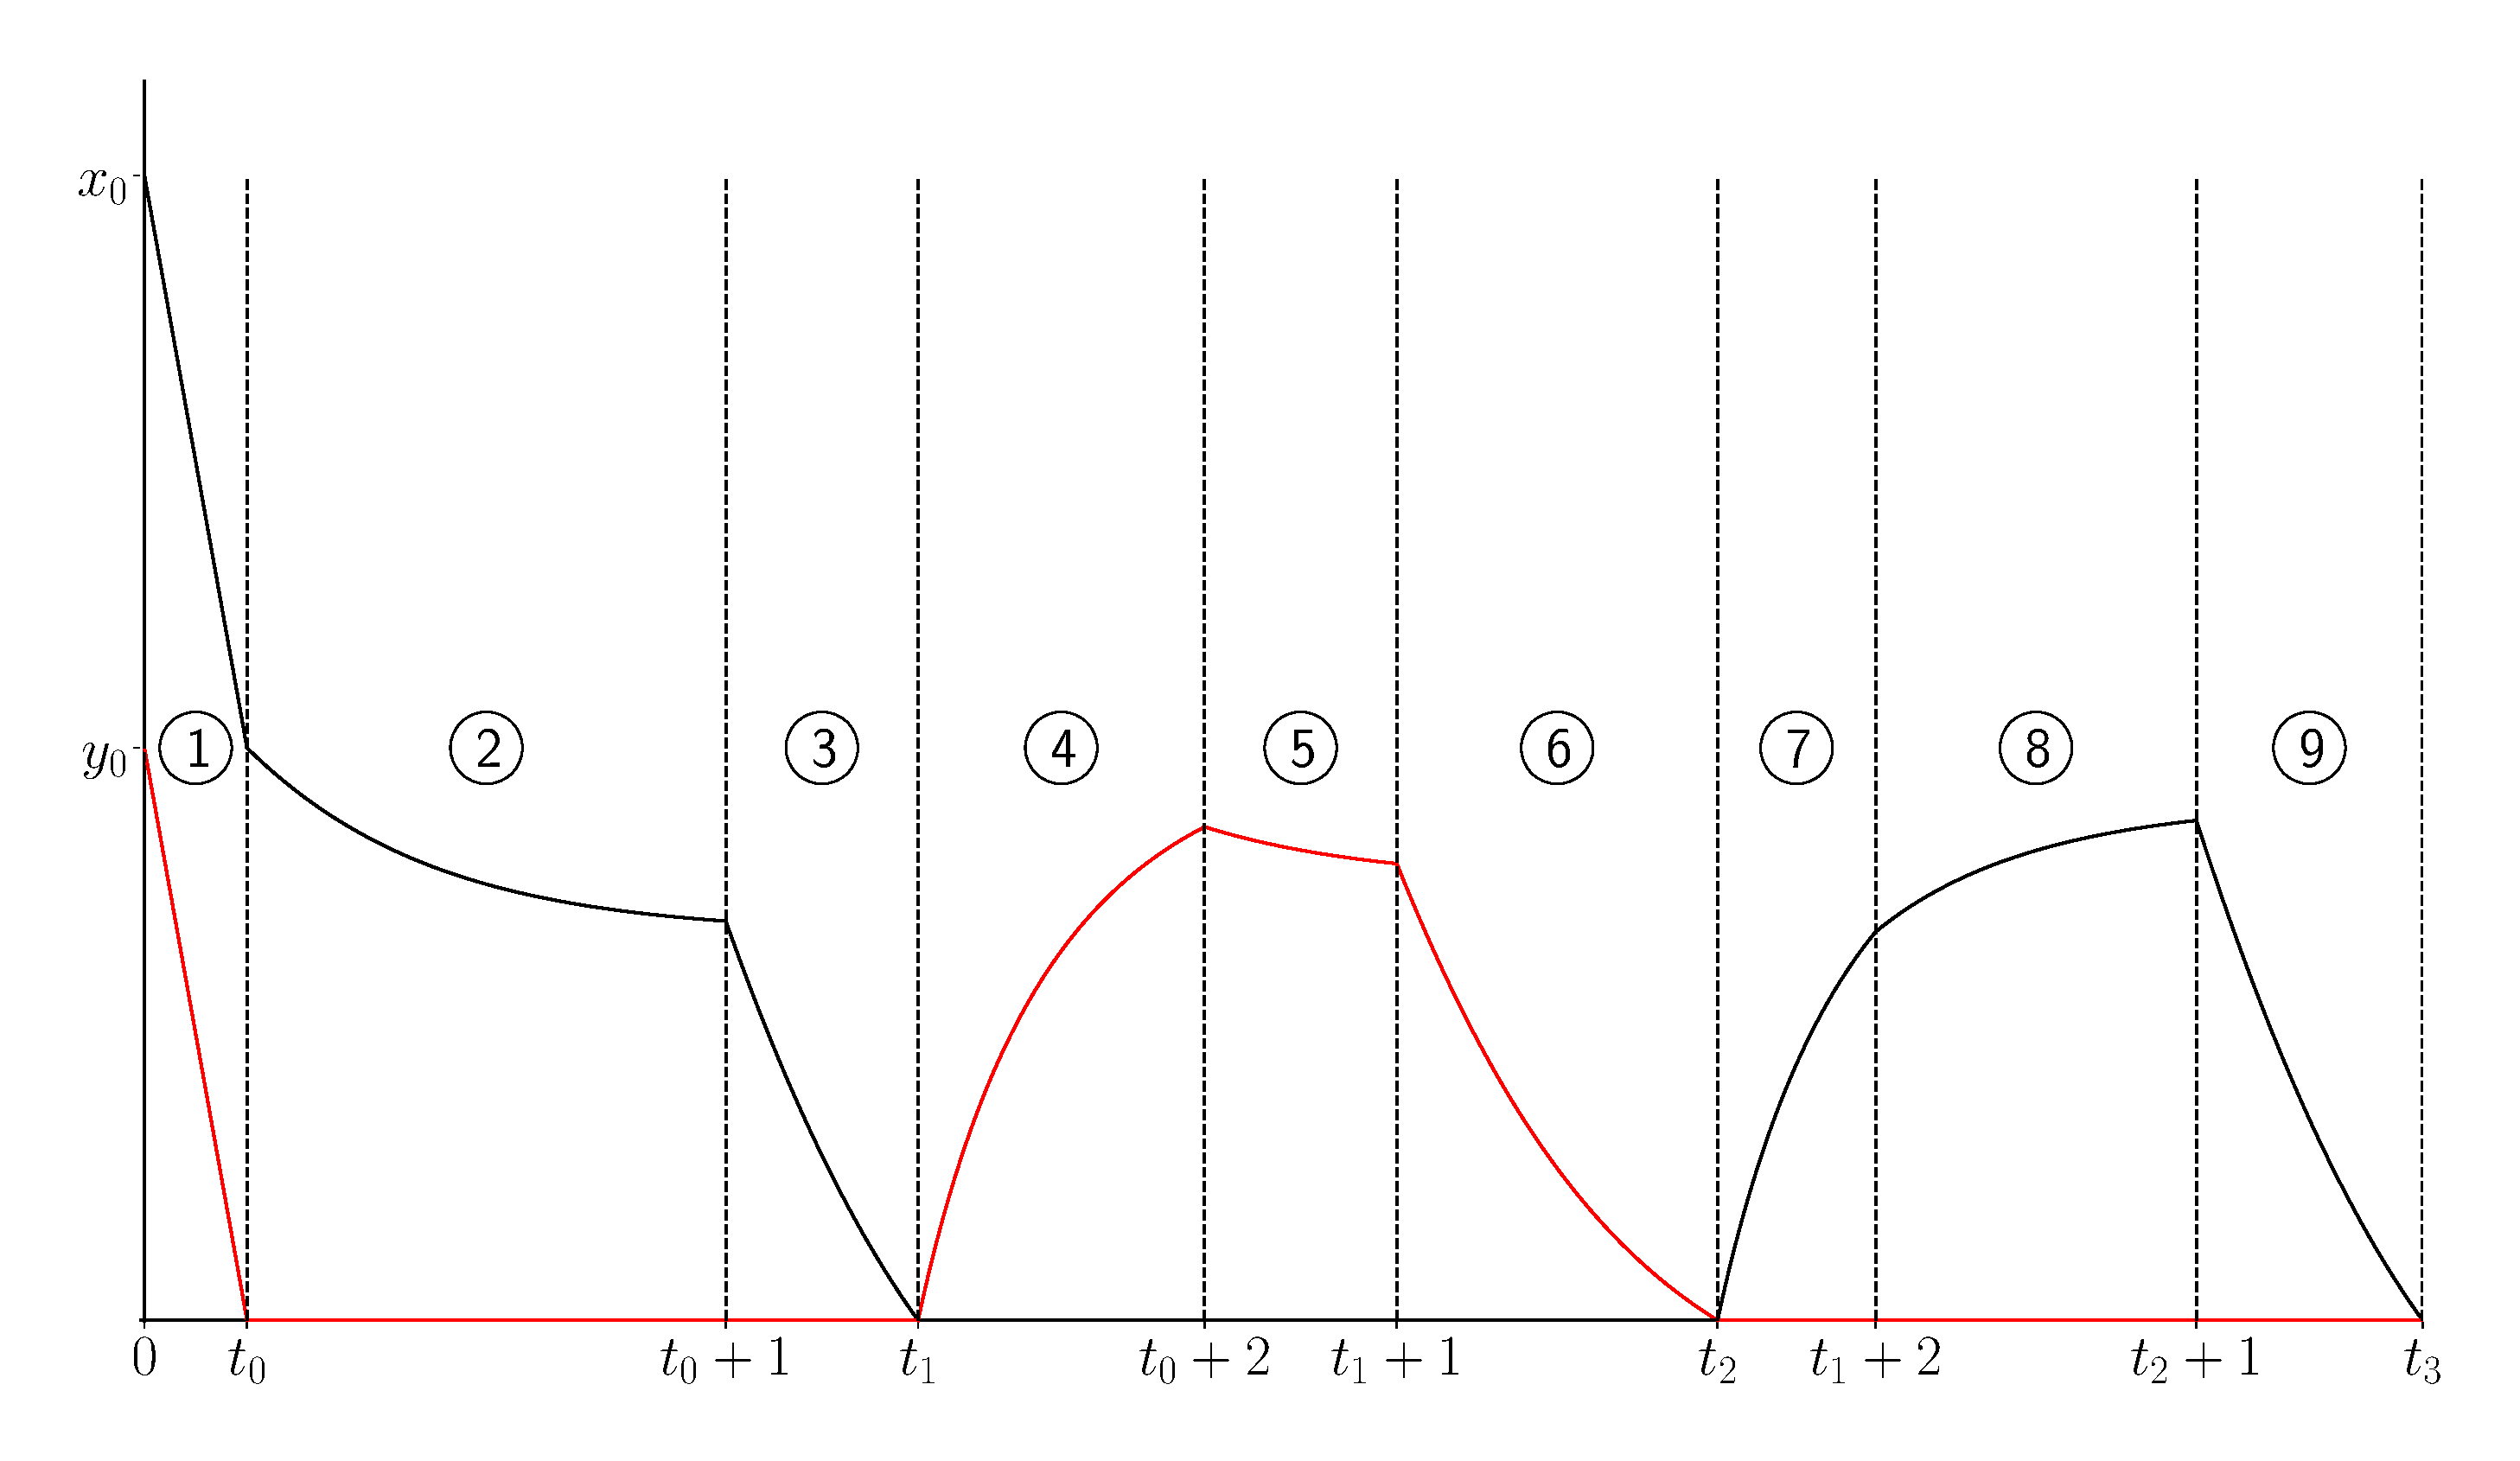
\includegraphics[width=\textwidth]{cluster_step_by_step.eps}
	\caption{Решение системы \eqref{eq:system_main_relay}, построенное методом шагов. Чёрная линия --- компонента решения $x$, красная линия --- компонента решения $y$. Числа в кругах означают номер шага построения.}
	\label{fig:cluster_step_by_step}
\end{figure}


\subsection{Метод шагов}
\paragraph{Шаг 1.} На отрезке $[0, t_0]$ система \eqref{eq:system_main_relay} принимает вид
%
\begin{equation}
	\label{eq:step1_system}
	\begin{cases}
		\dot{x} = -\beta,\\
		\dot{y} = -\beta.
	\end{cases}
\end{equation}

Она имеет решение \eqref{eq:step1_solution}, которое продолжается до точки $t_0 = \dfrac{y_0}{\beta}$, в которой $y(t_0) = 0$.

\paragraph{Шаг 2.} Рассмотрим следующий отрезок построения решения $[t_0, t_0 + 1]$. C учётом условия \eqref{eq:constraint_2}, при $y < 0$ второе уравнение системы \eqref{eq:system_main_relay} принимает вид
\[
\dot{y} = -\beta + \alpha \delta (n - 1) > 0,
\]
а при $y > 0$ получаем $\dot{y} = -\beta < 0$.

Следовательно, решение может быть продолжено только вдоль прямой $y = 0$ до момента, когда компонента $x$ также обратится в ноль. Иллюстрация динамики системы в точке $t= t_0$ приведена на рис. \ref{fig:dynamics_t0}. Система \eqref{eq:system_main_relay} принимает вид

\begin{equation}
	\label{eq:step2_system}
	\begin{cases}
		\dot{x} = -\beta + G(0, t) \alpha \delta n e^{-x},\\
		\dot{y} = -\beta + G(0, t) \alpha \delta (n - 1),
	\end{cases}
\end{equation}
%
Из второго уравнения и условия $\dot{y} = 0$ находим $G(0, t) = \frac{\beta}{\alpha \delta (n - 1)}$. Подставляя это значение в первое уравнение, получаем начальную задачу Коши
\begin{equation}
	\label{eq:step2_start}
	\dot{x} = -\beta + \beta\cdot\dfrac{n}{n - 1}e^{-x}, \quad x(t_0) = x_0 - \beta t_0.
\end{equation}

\begin{lemma}
	\label{lm:default_equation}
	Задача Коши 
	\[
	\dot{x} = -\beta + \beta \theta e^{-x}, \quad x \vert_{t = t_*} = x_*,
	\]
	где $\theta, x_*, t_*$ --- вещественные константы, имеет при $t > t_*$ решение 
	\[
	x = x_* - \beta (t - t_*) + \ln\left(1 + \theta e^{-x_*} (e^{\beta(t - t_*)} - 1)\right) =
	-\beta t + \ln\left(e^{x_* + \beta t_*} + \theta (e^{\beta t} - e^{\beta t_*})\right).
	\]
	%\[
	%x = -\beta t + \ln\left(e^{x_* + \beta t_*} + \theta (e^{\beta t} - e^{\beta %t_*})\right).
	%\]
\end{lemma}

\begin{proof}
	После замены $x = z - \beta t$, $z_* = z \vert_{t = t_*} = x_* + \beta t_*$ получаем уравнение с разделяющимися переменными
	\[
	e^{z} \dot{z} = \beta \cdot \theta e^{\beta t}.
	\]
	Интегрируя, получаем
	\[
	\int\limits_{z_*}^z e^{\tilde{z}} \, d\tilde{z} = \int\limits_{t_*}^{t} \beta \theta e^{\beta \tilde{t}}\,d\tilde{t},
	\]
	\[
	e^z - e^{z_*} = \theta (e^{\beta t} - e^{\beta t_*}).
	\]
	После обратной замены и элементарных преобразований получаем требуемое.
\end{proof}

Применяя лемму \ref{lm:default_equation} к уравнению \eqref{eq:step2_start} с условиями $\theta = \dfrac{n}{n - 1}$, $t_* = t_0$, $x_* = x_0 - \beta t_0$, получаем решение \eqref{eq:step2_solution}. Решение продолжается либо до точки $t_0 + 1$, либо до точки, в которой $x = 0$. Докажем, что всегда реализуется первый случай.

\begin{lemma}
	\label{lm:solution_monotone}
	Пусть $A, B$ --- вещественные константы такие, что $A + B e^{\beta t} > 0$ при $t > 0$. Функция $f(t) = -\beta t + \ln\left(A + B e^{\beta t}\right)$ монотонна на всей обрасти определения.
\end{lemma}
\begin{proof}
	Продифференцируем $f(t)$:
	\[
	f'(t) = -\beta + \beta \dfrac{B e^{\beta t}}{A + B e^{\beta t}} = -\dfrac{A \beta}{A + B e^{\beta t}}.
	\]
	Знаменатель по условию положителен, поэтому производная знакопостоянна и имеет тот же знак, что $-A \beta$. Следовательно, $f$ монотонна.
\end{proof}

По лемме \ref{lm:solution_monotone}, решение $x(t)$ на втором шаге монотонно. Чтобы убедиться, что оно положительно на отрезке $[t_0, t_0 + 1]$, достаточно проверить условие $x(t_0 + 1) > 0$.
%
\[
x(t_0 + 1) = x_0 - \beta (t_0 + 1) + \ln\left(1 + \frac{n}{n - 1}e^{-x_0 + \beta t_0} (e^{\beta} - 1)\right) > 0.
\]
%
После элементарных преобразований получаем неравенство
\[
e^{x_0 - \beta t_0} > \dfrac{n - e^\beta}{n - 1},
\]
которое верно, поскольку левая часть больше $1$, а правая --- меньше.

Следовательно, $x > 0$ на отрезке $[t_0, t_0 + 1]$.

\paragraph{Шаг 3.} На отрезке $[t_0 + 1, t_1]$ система \eqref{eq:system_main_relay} принимает вид
\begin{equation}
	\label{eq:system_step3}
	\begin{cases}
		\dot{x} = -\beta + \alpha \delta n e^{-x} G(0, t),\\
		\dot{y} = -\beta + \alpha \left(G(0, t - 1) + \delta (n - 1) G(0, t)\right).
	\end{cases}
\end{equation}

Учитывая условия $\dot{y} = 0$, $G(0, t - 1) = \frac{\beta}{\alpha \delta (n - 1)}$, из второго уравнения находим $G(0, t) = \frac{\beta}{\alpha} \cdot \frac{\delta(n - 1) - 1}{\delta^2 (n - 1)^2}$. Подставляя это значение в первое уравнение, получаем
\[
\dot{x} = -\beta + \beta \cdot \dfrac{n (\delta(n - 1) - 1)}{\delta (n - 1)^2} e^{-x}.
\]
%
Применяя лемму \ref{lm:default_equation} при $\theta = \frac{n (\delta(n - 1) - 1)}{\delta (n - 1)^2}$, получаем решение \eqref{eq:step3_solution} при $i = 0$.

Аналитический вид решения сохраняется до точки $t_0 + 2$ или до точки $t_1$, в которой $x(t_1) = 0$. По лемме \ref{lm:solution_monotone}, $x(t)$ монотонна на третье	м шаге. Следовательно, $t_1 \in (t_0 + 1, t_0 + 2)$ тогда и только тогда, когда $x(t_0 + 2) < 0$.

\begin{lemma}
	\label{lm:t1_one_step}
	Неравенство \eqref{eq:constraint_1} равносильно условию $t_1 \in (t_0 + 1, t_0 + 2)$.
\end{lemma}
\begin{proof}
	Подставим $t = t_0 + 1$ в \eqref{eq:step2_solution}:
	\begin{multline*}
		x(t_0 + 1) = x_0 - \beta (t_0 + 1) + \ln\left(1 + \frac{n}{n - 1} e^{-x_0 + \beta t_0}  (e^{\beta} - 1)\right) =\\= -\beta + \ln\left(e^{x_0 - y_0} + \dfrac{n}{n - 1}(e^{\beta} - 1)\right).
	\end{multline*}
	
	Подставим найденное значение $x(t_0 + 1)$ и $t = t_0 + 2$ в формулу \eqref{eq:step3_solution}:
	\small
	\begin{multline*}
		x(t_0 + 2) = -\beta (t_0 + 2) + \ln\left(e^{x(t_0 + 1) + \beta (t_0 + 1)} + \frac{n (\delta(n - 1) - 1)}{\delta (n - 1)^2} (e^{\beta (t_0 + 2)} - e^{\beta (t_0 + 1)})\right) = \\ = -2\beta + \ln\left(e^{x(t_0 + 1) + \beta} + \frac{n (\delta(n - 1) - 1)}{\delta (n - 1)^2} (e^{2\beta} - e^{\beta})\right) = \\ = -2\beta + \ln\left(e^{x_0 - y_0} + \dfrac{n}{n - 1}(e^{\beta} - 1) + \frac{n (\delta(n - 1) - 1)}{\delta (n - 1)^2} (e^{2\beta} - e^{\beta})\right).
	\end{multline*}
	\normalsize
	
	Неравенство $x(t_0 + 2) < 0$ эквивалентно \eqref{eq:constraint_1}, что можно проверить элементарными преобразованиями.
\end{proof}

\paragraph{Шаг 4.} На отрезке $[t_1, t_0 + 2]$ система \eqref{eq:system_main_relay} принимает вид
\small
\begin{equation}
	\begin{cases}
		\dot{x} = -\beta + \alpha \left(\delta (m - 1) G(x, t) + \delta n e^{y - x} G(y, t)\right)\\
		\dot{y} = -\beta + \alpha \left(e^{y(t - 1) - y} G(0, t - 1) + \delta m e^{x - y} G(x, t) + \delta (n - 1) G(y, t)\right).
	\end{cases}
\end{equation}
\normalsize
% Если $x < 0$, то из первого уравнения получаем $\dot{x} \geqslant -\beta + \alpha(m - 1) > 0$. По лемме \ref{lm:signed_solution}, $x \geq 0$. Если $x > 0$ в точке $\tau \in (t_1, t_0 + 2)$, то либо $y > 0$ и $\dot{x} = -\beta < 0$, либо $y = 0$ и система примет вид \eqref{eq:system_step3}, для которой также $\dot{x} < 0$. По лемме \ref{lm:signed_solution}, $x \leq 0$. Значит, на 4-м шаге $x \equiv 0$.

Если $x < 0$, то из первого уравнения получаем $\dot{x} \geqslant -\beta + \alpha \delta (m - 1) > 0$. Если $x > 0$ в точке $t \in (t_1, t_0 + 2)$, то либо $y > 0$ и $\dot{x} = -\beta < 0$, либо $y = 0$ и система примет вид \eqref{eq:system_step3}, для которой также $\dot{x} < 0$. Тогда решение может быть продолжено только вдоль прямой $x = 0$. Иллюстрация динамики системы в точке $t=t_1$ приведена на рис. \ref{fig:dynamics_t1}.

Система \eqref{eq:system_main_relay} примет вид
%
\begin{equation}
	\label{eq:step4_system}
	\begin{cases}
		\dot{x} = -\beta + \alpha \delta (m - 1) G(0, t),\\
		\dot{y} = -\beta + \alpha \left(e^{-y} G(0, t - 1) + \delta m e^{-y} G(0, t)\right).
	\end{cases}
\end{equation}
%
Из первого уравнения находим $G(0, t) = \frac{\beta}{\alpha \delta (m - 1)}$. С учётом $G(0, t - 1) = \frac{\beta}{\alpha \delta (n - 1)}$, первое уравнение примет вид
\[
\dot{y} = -\beta + \beta \left(\dfrac{1}{\delta(n - 1)} + \dfrac{m}{m - 1} \right) e^{-y}.
\]
%
Применяя лемму \ref{lm:default_equation} с условиями
\[
\theta = \dfrac{1}{\delta(n - 1)} + \dfrac{m}{m - 1}, \quad t_* = t_1, \quad y(t_*) = 0,
\]
получаем решение \eqref{eq:step4_solution} системы на отрезке $[t_1, t_0 + 2]$:

Легко проверить, что условие $y > 0$ для второго уравнения из \eqref{eq:step4_solution} эквивалентно верному неравенству
\[
\dfrac{1}{\delta(n - 1)} + \dfrac{m}{m - 1} > 1,
\]
поэтому новых точек переключения на отрезке $[t_1, t_0 + 2]$ не появляется.

\paragraph{Шаг 5.} На отрезке $[t_0 + 2, t_1 + 1]$ система имеет вид \eqref{eq:step4_system} с одним изменением: $G(0, t - 1) = \frac{\beta}{\alpha} \cdot \frac{\delta(n - 1) - 1}{\delta^2 (n - 1)^2}$.
%
Тогда на 5-м шаге система имеет решение \eqref{eq:step5_solution}.
%
Как и в прошлом случае, убедимся, что $y > 0$. Действительно, условие $y > 0$ для второго уравнения из \eqref{eq:step5_solution} эквивалентно
\[
\frac{\delta(n - 1) - 1}{\delta^2 (n - 1)^2} + \dfrac{m}{m - 1} > \dfrac{e^{\beta t} - e^{y(t_0 + 2) + \beta (t_0 + 2)}}{e^{\beta t} - e^{\beta (t_0 + 2)}},
\]
что верно, поскольку левая часть больше $1$, а правая --- меньше.

\paragraph{Шаг 6 и последующие шаги.} Поскольку $G(0, t) = \frac{\beta}{\alpha \delta (m - 1)}$ на промежутке $[t_1, t_1 + 1]$, следующая точка переключения --- либо $t_1 + 2$, либо $t_2 \in (t_1 + 1, t_1 + 2)$ при условии $y(t_2) = 0$. Предположим, что реализуется второй случай; соответствующие ограничения на параметры сформулируем и докажем позже.

Тогда при $t \in [t_1 + 1, t_2]$ система \eqref{eq:system_main_relay} имеет вид
%
\begin{equation}
	\label{eq:step6_system}
	\begin{cases}
		\dot{x} = -\beta + \alpha \left(\frac{\beta}{\alpha \delta (m - 1)} + \delta (m - 1) G(0, t)\right)\\
		\dot{y} = -\beta + \alpha \delta m e^{-y} G(0, t).
	\end{cases}
\end{equation}
%
Заметим, что он совпадает с системой \eqref{eq:system_step3} с точностью до замены $x$ на $y$, $m$ и $n$, и начального значения $y(t_1 + 1)$. Значит, следующие шаги построения решения аналогичны шагам 3~--~5. Общий вид решения на отрезках $[t_1 + 1, t_2]$, $[t_2, t_1 + 2]$, $[t_1 + 2, t_2 + 1]$ приведён в формулах \eqref{eq:step6_solution}, \eqref{eq:step7_solution},  \eqref{eq:step8_solution}.

При условии, что компонента $x$ обращается в ноль в точке $t_3 \in (t_2 + 1, t_2 + 2)$, решение на отрезке $[t_2 + 1, t_3]$ описывается формулами \eqref{eq:step9_solution} для $i = 0$.

Построение решения на следующих шагах, соответствующих $i \geqslant 1$ в условии теоремы \ref{thm:relay_solution}, в точности повторяет шаги, начиная с 4-го.

\subsection{Ограничения на параметры системы}
Опишем достаточные условия на параметры, гарантирующие $t_{i + 1} \in (t_i + 1, t_i + 2)$ при $i \geqslant 1$.

Обозначим (см. рисунок \ref{fig:x_star})
\begin{equation}
	\label{eq:x_star_definition}
	x^*_i = x(t_{2i} + 1), \quad y^*_i = y(t_{2i - 1} + 1).
\end{equation}

\begin{figure}
	\centering
	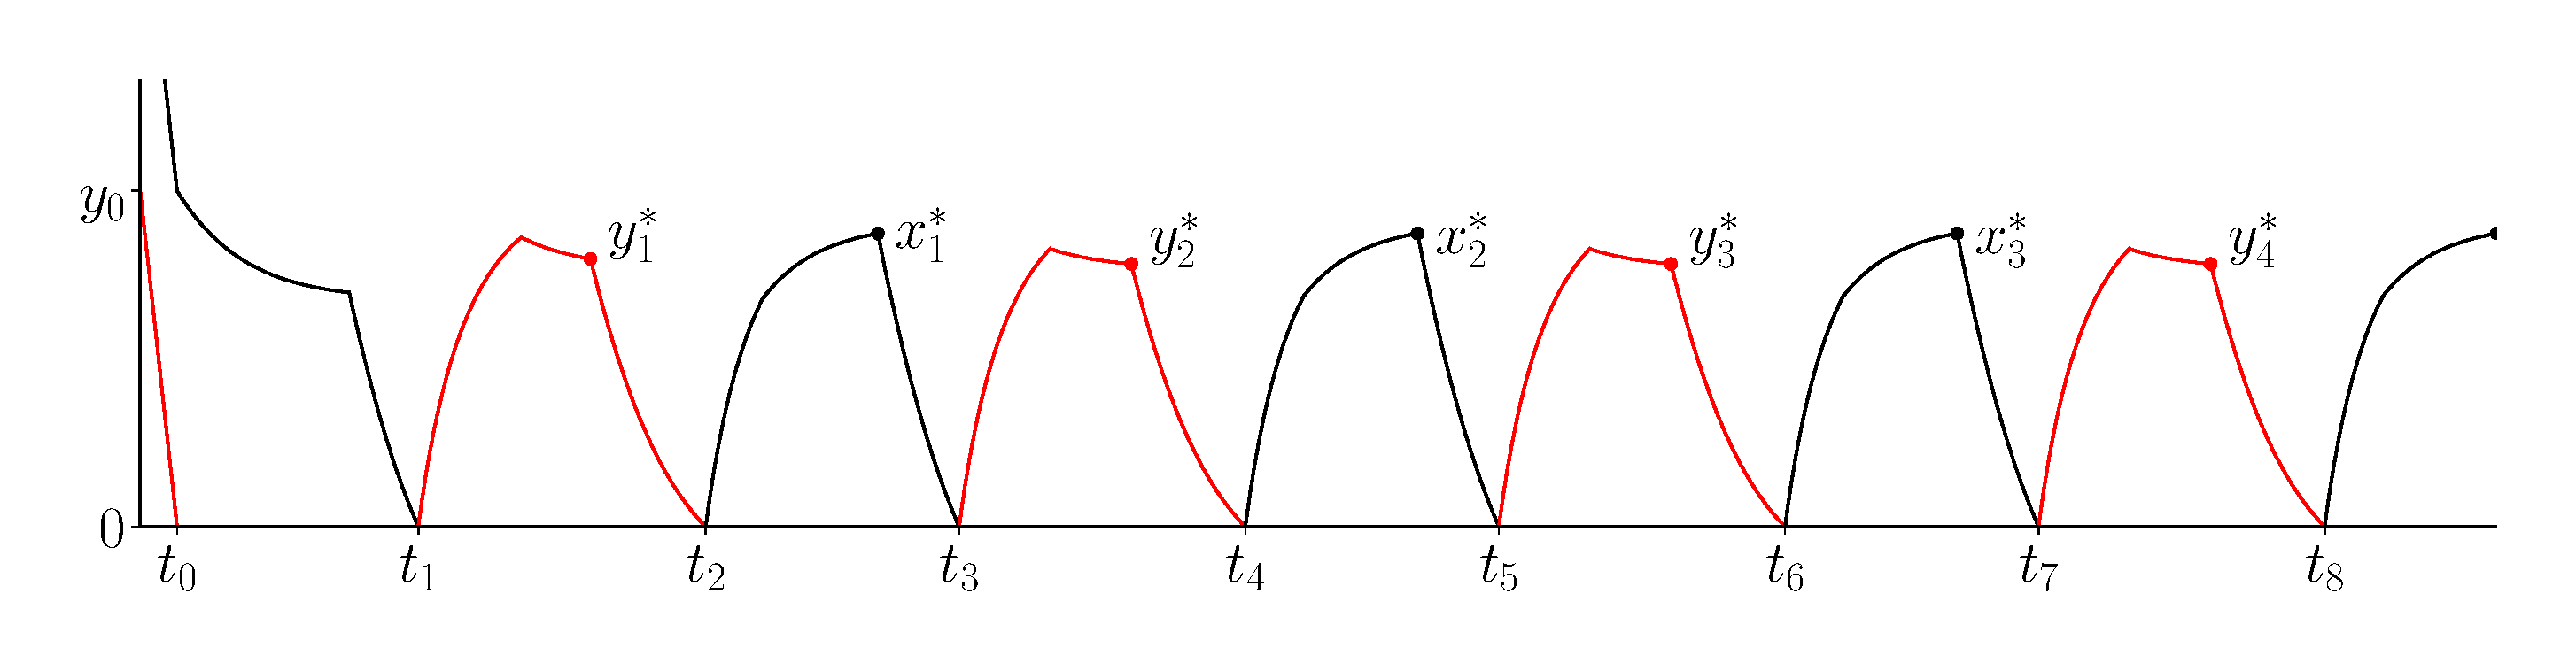
\includegraphics[width=\textwidth]{cluster_stars.eps}
	\caption{Последовательности значений $x^*_i$ и $y^*_i$, определённые формулами \eqref{eq:x_star_definition}. По каждому из значений решение системы \eqref{eq:system_main_relay} продолжается однозначно. В лемме \ref{lm:convergence_x_star} доказывается сходимость этих последовательностей.}
	\label{fig:x_star}
\end{figure}

\begin{figure}
	\begin{minipage}{0.48\textwidth}
		\centering
		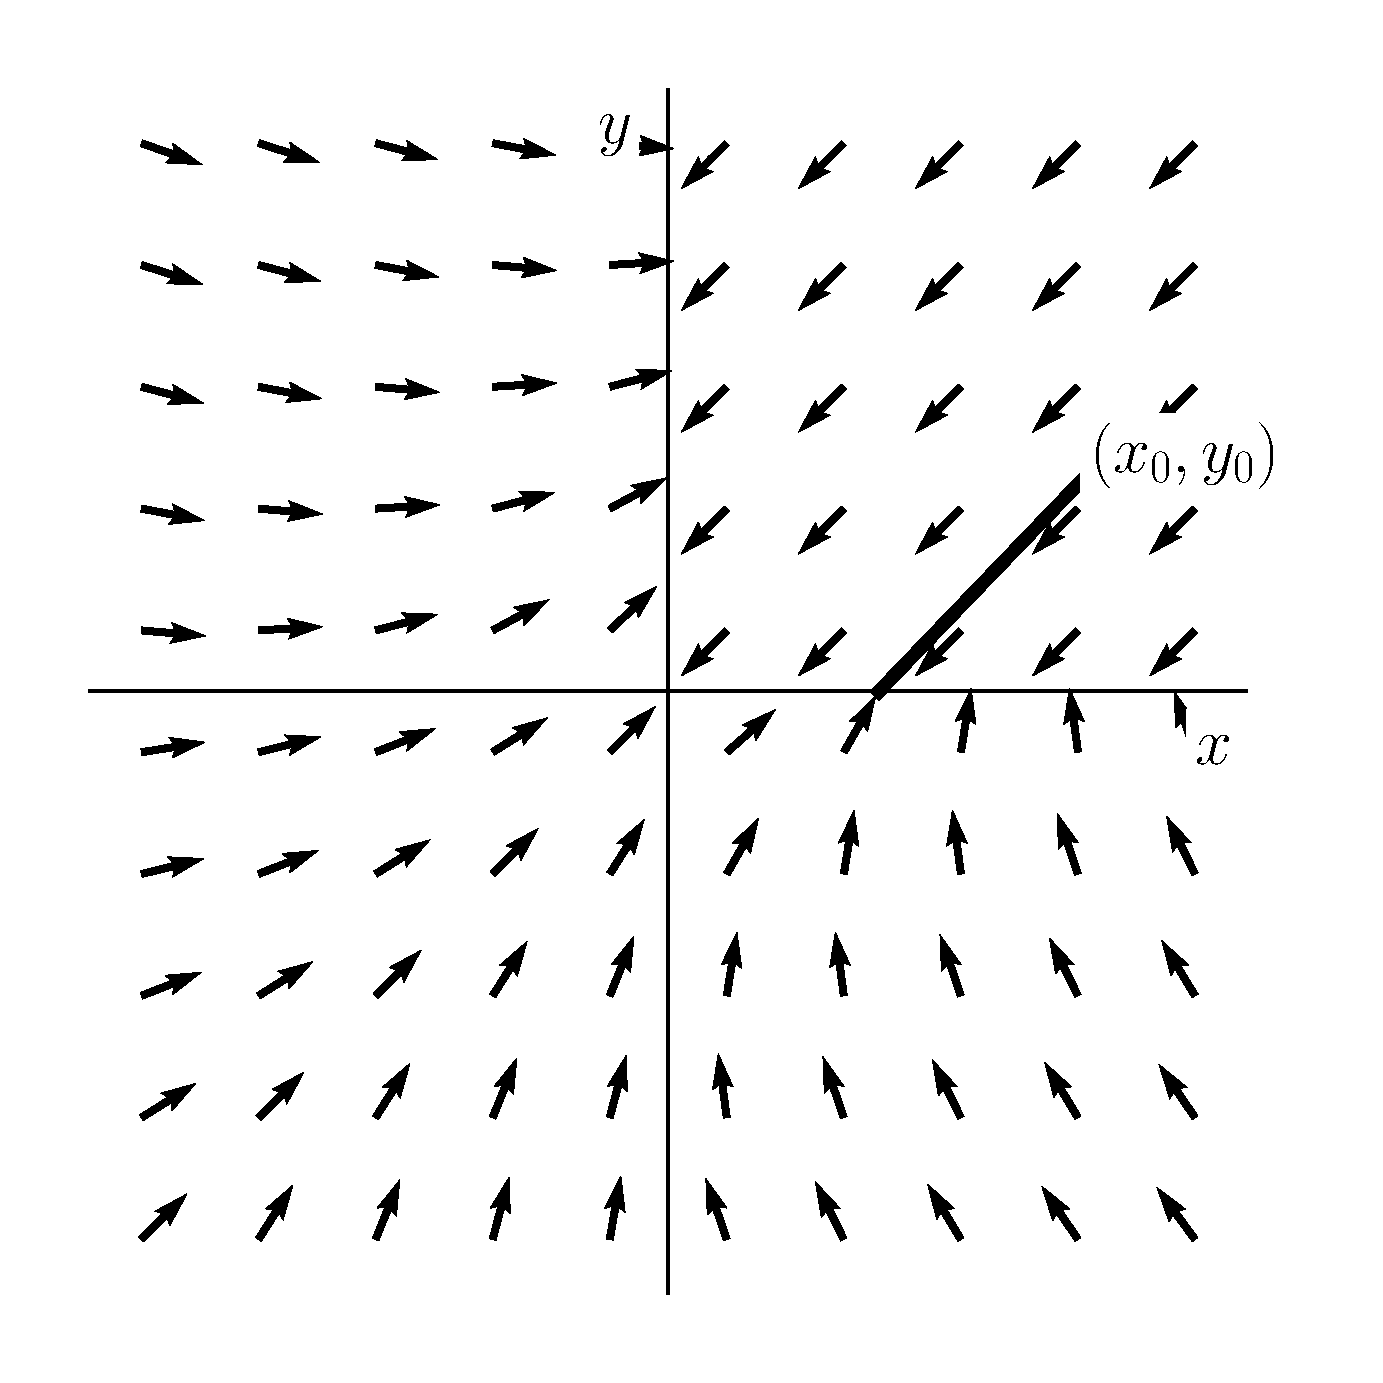
\includegraphics[width=\linewidth]{cluster_dynamics_t0.eps}
		\captionsetup{width=0.9\textwidth} 
		\caption{Векторное поле $(\dot{x}, \dot{y})$ в момент времени $t = t_0$. Жирной линией изображена проекция фазовой траектории на плоскость $(x, y)$ при $t \in [0, t_0]$. %Поскольку с обеих сторон прямой $y = 0$ векторы $(\dot{x}, \dot{y})$ направлены к ней, решение продолжается вдоль прямой.
		}
		\label{fig:dynamics_t0}
	\end{minipage}\hfill
	\begin{minipage}{0.48\textwidth}
		\centering
		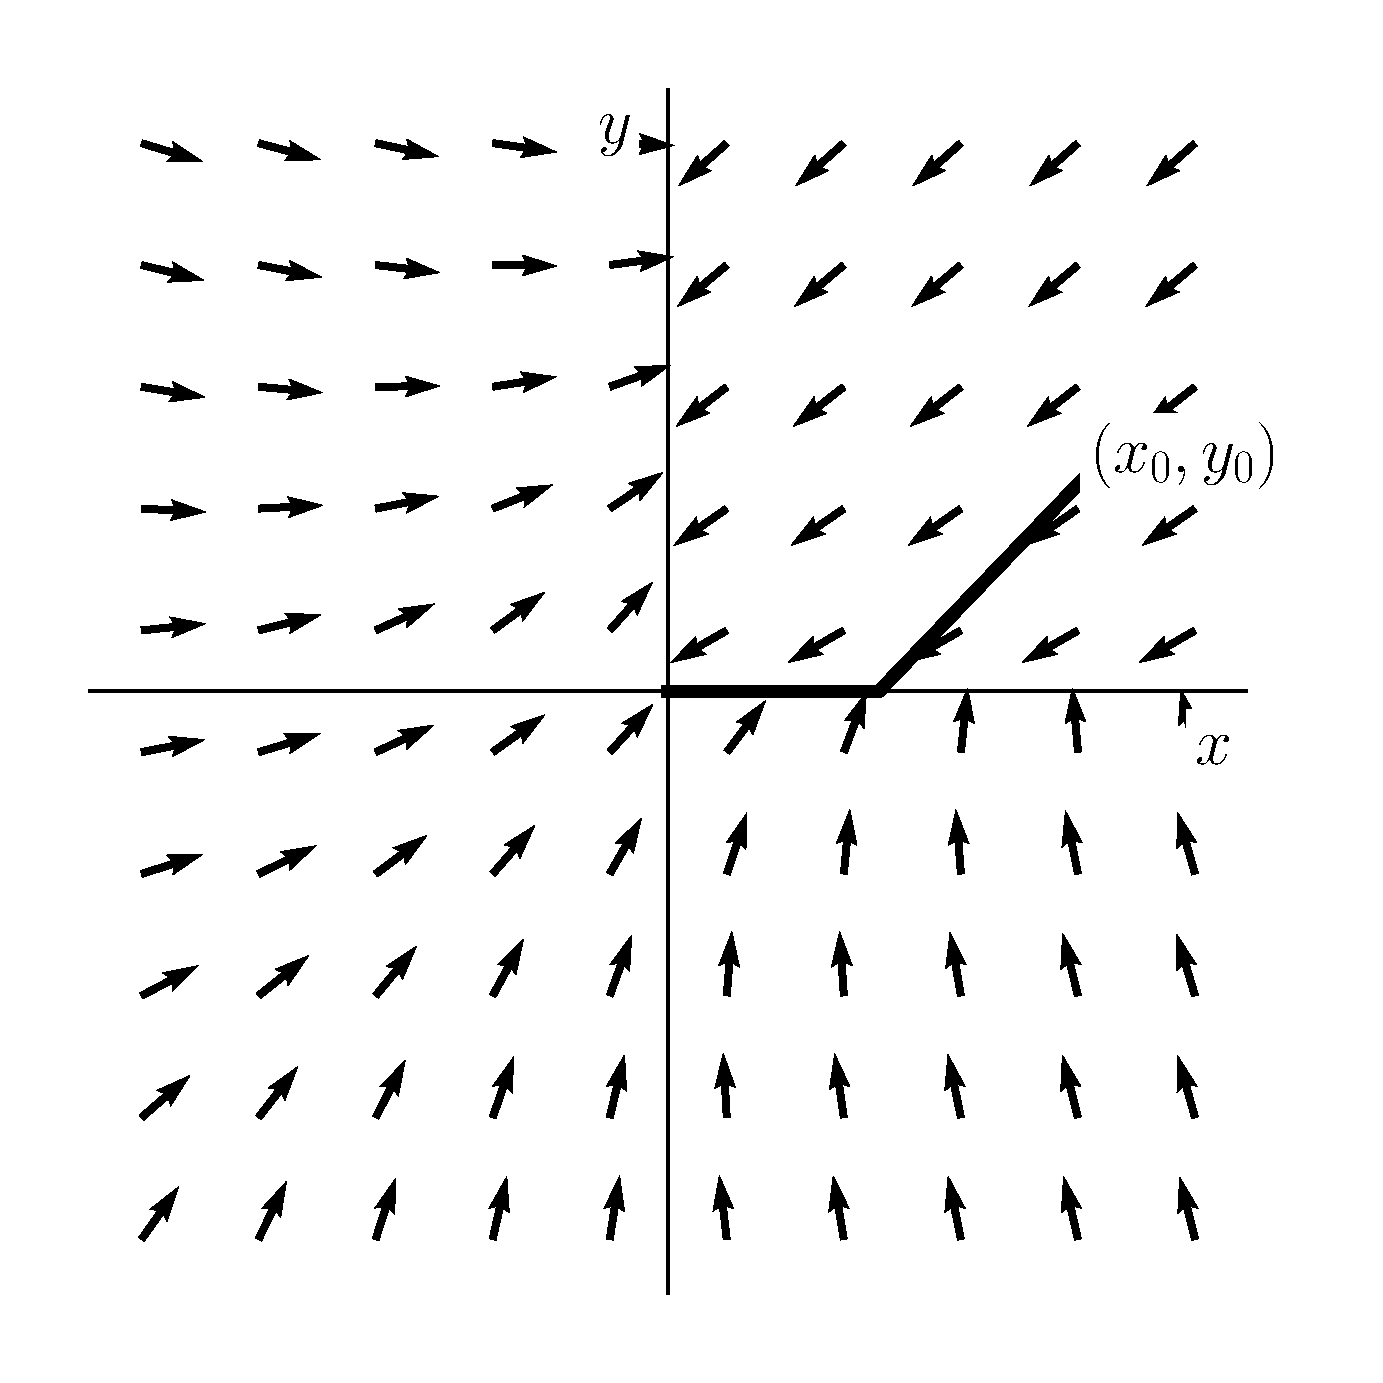
\includegraphics[width=\linewidth]{cluster_dynamics_t1.eps}
		\captionsetup{width=0.9\textwidth} 
		\caption{Векторное поле $(\dot{x}, \dot{y})$ в момент времени $t = t_1$. Жирной линией изображена проекция фазовой траектории на плоскость $(x, y)$ при $t \in [0, t_1]$.}
		\label{fig:dynamics_t1}
	\end{minipage}
\end{figure}

\begin{lemma}
	\label{lm:xy_star_bounds}
	При условии $t_{i + 1} \in (t_i + 1, t_i + 2)$ для любого $i \geqslant 1$ верны следующие оценки:
	\footnotesize
	\begin{multline}
		\label{eq:x_star_bound}
		-\beta + \ln\left(1 + \left( \frac{\delta(m - 1) - 1}{\delta^2 (m - 1)^2} + \dfrac{n}{n - 1} \right)(e^{\beta} - 1) \right) < x^*_i < \\ -\beta + \ln\left(1 + \left( \dfrac{1}{\delta(m - 1)} + \dfrac{n}{n - 1} \right)(e^{\beta} - 1) \right)
	\end{multline}
	\begin{multline}
		\label{eq:y_star_bound}
		-\beta + \ln\left(1 + \left( \frac{\delta(n - 1) - 1}{\delta^2 (n - 1)^2} + \dfrac{m}{m - 1} \right)(e^{\beta} - 1) \right) < y^*_i < \\ -\beta + \ln\left(1 + \left( \dfrac{1}{\delta(n - 1)} + \dfrac{m}{m - 1} \right)(e^{\beta} - 1) \right)
	\end{multline}
	\normalsize
\end{lemma}
\begin{proof}
	Рассмотрим отрезок $[t_2, t_2 + 1]$.
	
	На отрезке $[t_2, t_1 + 2]$ действуют формулы \eqref{eq:step7_solution}. Пусть $\tau = t - t_2$, тогда
	%
	\[
	x(t_2 + \tau) = - \beta \tau + \ln\left( 1 + \left(\dfrac{1}{\delta(m - 1)} + \dfrac{n}{n - 1}\right) (e^{\beta \tau} - 1) \right).
	\]
	Пусть $\tau^* = t_1 + 2 - t_2$, тогда
	\[
	x(t_1 + 2) = x(t_2 + \tau^*) = -\beta \tau^* + \ln\left( 1 + \left(\dfrac{1}{\delta(m - 1)} + \dfrac{n}{n - 1}\right) (e^{\beta \tau^*} - 1) \right).
	\]
	
	На отрезке $[t_1 + 2, t_2 + 1]$ действуют формулы \eqref{eq:step8_solution}. Подставим вычисленное значение $x^* = x(t_1 + 2)$ и вычислим $x^*_1 = x(t_2 + 1)$:
	%
	\begin{multline}
		\label{eq:tau_to_t2+1}
		x^*_1 = x(t_2 + 1) = -\beta + \ln\Bigg( 1 - \left(\frac{1}{\delta(m - 1)} + \frac{n}{n - 1}\right) + \\ + \left(\frac{n}{n - 1} + \frac{\delta(m - 1) - 1}{\delta^2 (m - 1)^2}\right) e^{\beta} + \left(\frac{1}{\delta(m - 1)} - \frac{\delta(m - 1) - 1}{\delta^2 (m - 1)^2}\right) e^{\beta \tau^*} \Bigg).
	\end{multline}
	%
	Заметим, что 
	\[
	\frac{1}{\delta(m - 1)} - \frac{\delta(m - 1) - 1}{\delta^2 (m - 1)^2} = \frac{1}{\delta^2 (m - 1)^2} > 0,
	\]
	поэтому функция \eqref{eq:tau_to_t2+1} возрастает по $\tau^* \in [0, 1]$, следовательно, 
	%
	\[
	x^*_1 \vert_{\tau^* = 0} < x^*_1 < x^*_1 \vert_{\tau^* = 1}
	\]
	Вычисляя явно, получаем оценки \eqref{eq:x_star_bound} для $x_1^*$. Оценки \eqref{eq:x_star_bound} и \eqref{eq:y_star_bound} для $x_i^*$ и $y_i^*$ получаются аналогично. 
	
\end{proof}

\begin{lemma}
	\label{lm:constraints_all}
	Пусть верны ограничения \eqref{eq:constraint_1}, \eqref{eq:constraint_2}, \eqref{eq:constraint_3}. Тогда $t_{i + 1} \in (t_i + 1, t_i + 2)$ при любом целом $i \geqslant 0$.
\end{lemma}
\begin{proof}
	
	База индукции $t_1 \in (t_0 + 1, t_0 + 2)$ доказана в лемме \eqref{lm:t1_one_step}. Индукция заключается в последовательной проверке условий $y(t_{2i - 1} + 2) < 0$ на шаге \eqref{eq:step6_solution} и $x(t_{2i} + 2) < 0$ на шаге \eqref{eq:step9_solution} при любом $i \geqslant 1$.
	
	Не ограничивая общности, рассмотрим условие $y(t_1 + 2) < 0$. Из формул \eqref{eq:step6_solution} получаем:
	\[
	y(t_1 + 2) = -\beta + \ln\left(e^{y_1^*} + \frac{m(\delta(m - 1) - 1)}{\delta (m - 1)^2}(e^\beta - 1) \right).
	\]
	Поскольку справедлива оценка сверху из \eqref{eq:y_star_bound}, для выполнения $y(t_1 + 2) < 0$ достаточно
	%
	\small
	\[
	-\beta + \ln\Bigg(e^{-\beta} \left(1 + \left( \dfrac{1}{\delta(n - 1)} + \dfrac{m}{m - 1} \right)(e^{\beta} - 1)\right) + \frac{m(\delta(m - 1) - 1)}{\delta (m - 1)^2} (e^\beta - 1) \Bigg) < 0.
	\]
	\normalsize
	%
	Элементарными преобразованиями получаем второе неравенство \eqref{eq:constraint_3} для $y_1^*$. Аналогично, неравенство $x(t_2 + 2) < 0$ следует из первого неравенства \eqref{eq:constraint_3}, далее по индукции.
\end{proof}

\subsection{Доказательство теоремы \ref{thm:relay_solution}} 
Методом шагов были получены формулы \eqref{eq:step1_solution} -- \eqref{eq:step9_solution} в предположении $t_{i + 1} \in (t_i + 1, t_i + 2)$ при любом $i \geqslant 0$. В лемме \ref{lm:constraints_all} доказано, что справедливость этого предположения следует из ограничений \eqref{eq:constraint_1} и \eqref{eq:constraint_3}, поэтому теорема \ref{thm:relay_solution} доказана.


%%%%%%%%%%%%%%%%%%%%%%%%%%%%%%%%%%%%%%%%%%%
\section{Существование периодического решения}\label{sec:ch3/sect4}
%%%%%%%%%%%%%%%%%%%%%%%%%%%%%%%%%%%%%%%%%%%

\begin{lemma}
	\label{lm:convergence_x_star}
	Пусть выполнены условия теоремы \ref{thm:relay_solution}. Тогда последовательности $x^*_i$ и $y^*_i$, определённые формулами \eqref{eq:x_star_definition}, сходятся.
\end{lemma}
\begin{proof}
	
	Рассмотрим последовательность $x^*_i$. Докажем, что последовательность $x^*_i$ ограничена и монотонна для достаточно больших $i$.
	
	Решение системы определяет отображение
	\begin{equation}
		\label{eq:flow_relay}
		\Phi: x^*_i \mapsto x^*_{i + 1}.
	\end{equation}
	
	Докажем, что $\Phi$ возрастает. Разложим $\Phi$ в композицию отображений
	\begin{equation}
		x^*_i \mapsto t_{2i + 1} \mapsto y^*_{i + 1} \mapsto t_{2i + 2} \mapsto x^*_{i + 1}.
	\end{equation}
	
	Отображения $x^*_i \mapsto t_{2i + 1}$ и $y^*_{i + 1} \mapsto t_{2i + 2}$ возрастают из условия непересечения интегральных кривых на каждом шаге решения.
	
	Пусть $\tau^* = t_{2i} + 2 - t_{2i + 1} $. Поскольку $t_{2i + 1} \in (t_{2i} + 1, t_{2i} + 2)$, $\tau^* \in (0, 1)$. Значение $y^*_{i + 1}$ выражается через $\tau^*$ аналогично \eqref{eq:tau_to_t2+1}
	\footnotesize
	\[
	y^*_{i + 1} = -\beta + \ln\Bigg( 1 - \left(\frac{1}{\delta(n - 1)} + \frac{m}{m - 1}\right) +  e^{\beta} \left(\frac{m}{m - 1} + \frac{\delta(n - 1) - 1}{\delta^2 (n - 1)^2}\right) +  \frac{e^{\beta \tau^*}}{\delta^2 (n - 1)^2} \Bigg).
	\]
	\normalsize
	
	Поскольку коэффициент $\frac{1}{\delta^2 (n - 1)^2}$ при $e^{\beta \tau^*}$ положителен, $y^*_{i + 1}$ возрастает по переменной $\tau^*$, соответственно, отображение $t_{2i + 1} \mapsto y^*_{i + 1}$ убывает.
	
	Аналогично, убывает отображение $t_{2i + 2} \mapsto x^*_{i + 1}$. Следовательно, $\Phi$ возрастает как композиция двух возрастающих и двух убывающих отображений.
	
	Пусть $x^*_2 > x^*_1$. Тогда по индукции
	\[
	x^*_{i} > x^*_{i - 1} \Rightarrow \Phi(x^*_i) > \Phi(x^*_{i - 1}), \text{ т.~е. } x^*_{i + 1} > x^*_{i},
	\]
	следовательно, $x^*_i$ возрастает. Аналогично, если $x^*_2 < x^*_1$, то $x^*_i$ убывает, а если $x^*_2 = x^*_1$, то $x^*_i = x^*_1$ при любом $i$. Ограниченность $x^*_i$ следует из леммы \ref{lm:xy_star_bounds}. Следовательно, $x^*_i$ сходится. Аналогично, сходится последовательность $y^*_i$.
\end{proof}


\begin{theorem}
	\label{thm:periodic_relay_existence}
	При ограничениях \eqref{eq:constraint_1}, \eqref{eq:constraint_2}, \eqref{eq:constraint_3} система \eqref{eq:system_main_relay} имеет периодическое решение, описываемое на периоде $[t_1, t_3]$ формулами \eqref{eq:step4_solution} -- \eqref{eq:step9_solution}.
\end{theorem}
\begin{proof}
	Рассмотрим последовательность $x^*_i$, пусть $x^*_i \to x^*$. По построению, отображение $\Phi$ из леммы \ref{lm:convergence_x_star} непрерывно, поэтому
	\[
	x^*_{i + 1} = \Phi(x^*_i) \Rightarrow x^* = \Phi(x^*).
	\]
	Поскольку значение $x^*_1 = x(t_2 + 1)$ однозначно определяет решение при $t > t_2 + 1$, положив $x^*_1 = x^*$, получим периодическое решение, описываемое на периоде формулами \eqref{eq:step4_solution} -- \eqref{eq:step9_solution}.
\end{proof}

%%%%%%%%%%%%%%%%%%%%%%%%%%%%%%%%%%%%%%%%%%%
\section{Результаты численного моделирования}\label{sec:ch3/sect5}
%%%%%%%%%%%%%%%%%%%%%%%%%%%%%%%%%%%%%%%%%%%

На рисунке \ref{fig:cluster_solution} приведены решения релейной системы \eqref{eq:system_main_relay} в сравнении с решениями соответствующих систем при различных $\gamma$. Численный эксперимент показал, что решение релейной системы \eqref{eq:system_main_relay} стремится к соответствующему решению системы \eqref{eq:system_main} при $\gamma \to +\infty$.

На рисунке \ref{fig:cluster_solution2} приведены решения релейной системы \eqref{eq:system_main_relay} для значений параметров, не удовлетворяющих условию \eqref{eq:constraint_3} (сверху) или условию \eqref{eq:constraint_2} (снизу). В обоих случаях, решение оказывается близко к периодическому.

%На рисунке \ref{fig:cluster_solution} приведено решение релейной системы \eqref{eq:system_main_relay} в сравнение с решением соответствующей системы при различных $\gamma$. Численный эксперимент показал, что решение релейной системы \ref{eq:system_main_relay} стремится к соответствующему решению системы \eqref{eq:system_main} при $\gamma \to +\infty$.

На рисунке \ref{fig:phase_portrait} приведён портрет системы \eqref{eq:system_main_relay} при различных значениях $\gamma$ в псевдофазовом пространстве (в координатах $x, y$). При $\gamma \to +\infty$ портрет вырождается в пару отрезков.

\begin{figure}[!htb]
	\centering
	
	\includegraphics[width=0.9\linewidth]{cluster_solution_1.eps}
	
	\smallskip
	
	\includegraphics[width=0.9\linewidth]{cluster_solution_2.eps}
	
	\caption{Решения системы \eqref{eq:system_main} для значений параметров $\alpha = 5.0$, $\beta = 3.7$, $m = 3$, $n = 4$, $\delta = 1.2$  (сверху); $\alpha = 3.0$, $\beta = 2.1$, $m = 2$, $n = 2$, $\delta = 1.5$ (снизу). Сплошными линиями изображены решения релейной системы \eqref{eq:system_main_relay}, штриховыми линиями --- решения системы при $\gamma = 200$, штрих-пунктирными линиями --- решения при $\gamma = 20$.
	}
	\label{fig:cluster_solution}
\end{figure}

\begin{figure}[!htb]
	\centering
	\includegraphics[width=0.9\linewidth]{cluster_solution_3.eps}
	
	\smallskip
	
	\includegraphics[width=0.9\linewidth]{cluster_solution_4.eps}
	
	\caption{Решения системы \eqref{eq:system_main} для значений параметров $\alpha = 10.0$, $\beta = 1.0$, $m = 5$, $n = 4$, $\delta = 1.02$, $\gamma = 500$ (сверху); $\alpha = 6.0$, $\beta = 1.6$, $m = 4$, $n = 3$, $\delta = 1.1$, $\gamma = 100$ (снизу).}
	\label{fig:cluster_solution2}
\end{figure}

\begin{figure}[!htb]
	\centering
	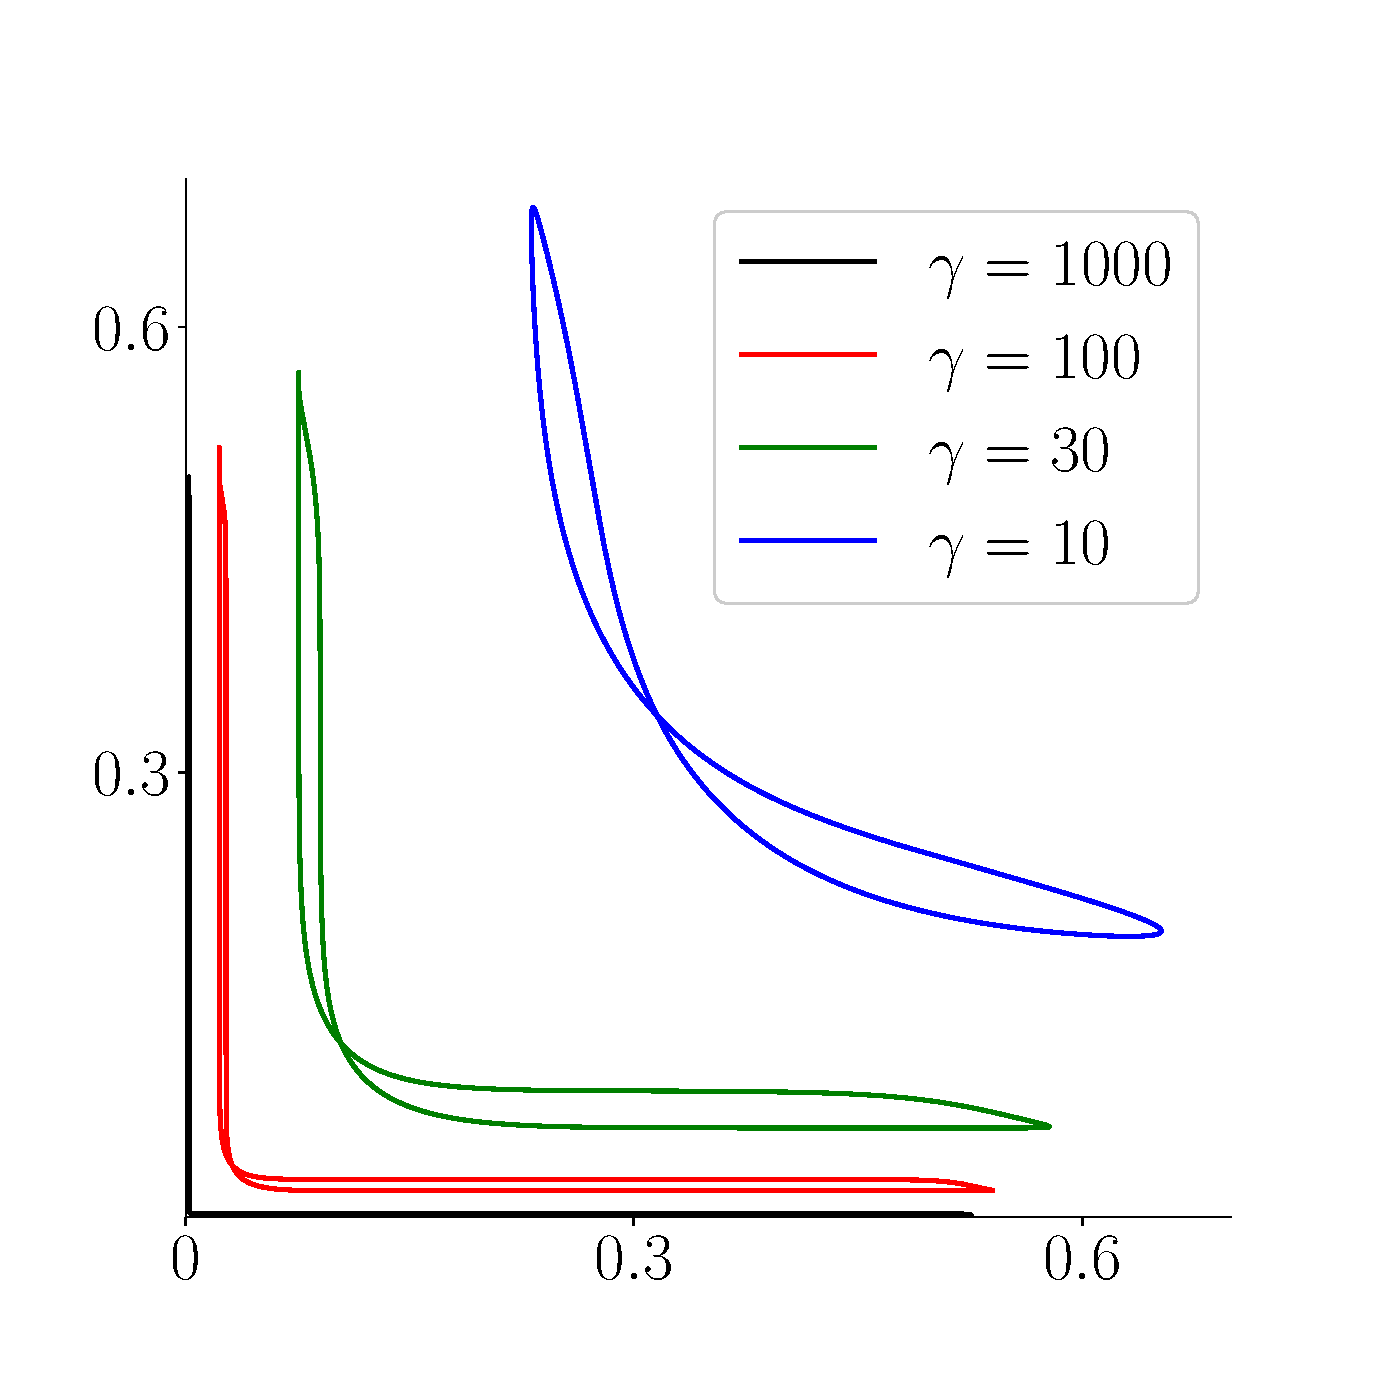
\includegraphics[width=0.5\linewidth]{cluster_phase_portrait.eps}
	\caption{Псевдофазовый портрет периодического решения системы \eqref{eq:system_main} при различных значениях $\gamma$. При $\gamma \gg 1$ портрет <<прижимается>> к координатным осям.}
	\label{fig:phase_portrait}
\end{figure} 

%%%%%%%%%%%%%%%%%%%%%%%%%%%%%%%%%%%%%%%%%%%
\section{Выводы к главе 3}\label{sec:ch3/sect6}
%%%%%%%%%%%%%%%%%%%%%%%%%%%%%%%%%%%%%%%%%%%
В данной главе было показано существование периодических режимов с кластерной синхронизацией в релейной системе генераторов Мэки-Гласса, а также дано их аналитическое описание.

Отметим, что возможно рассмотрение более общего случая: можно опустить требование $t_{i + 1} \in (t_{i} + 1, t_{i} + 2)$, при этом аналитический вид решения также представляется явно. Численное моделирование показывает существование периодических режимов в этом случае, однако доказательство его существования аналогично лемме \ref{lm:convergence_x_star} не обобщается ввиду немонотонности отображения $\Phi$. Также возможно построение решения с другими начальными условиями и ограничениями на параметры. Эти обобщения представляют интерес для дальнейших исследований.
           % Глава 3
\chapter*{Заключение}                       % Заголовок
\addcontentsline{toc}{chapter}{Заключение}  % Добавляем его в оглавление

%% Согласно ГОСТ Р 7.0.11-2011:
%% 5.3.3 В заключении диссертации излагают итоги выполненного исследования, рекомендации, перспективы дальнейшей разработки темы.
%% 9.2.3 В заключении автореферата диссертации излагают итоги данного исследования, рекомендации и перспективы дальнейшей разработки темы.
%% Поэтому имеет смысл сделать эту часть общей и загрузить из одного файла в автореферат и в диссертацию:

Основные результаты работы заключаются в следующем.
%% Согласно ГОСТ Р 7.0.11-2011:
%% 5.3.3 В заключении диссертации излагают итоги выполненного исследования, рекомендации, перспективы дальнейшей разработки темы.
%% 9.2.3 В заключении автореферата диссертации излагают итоги данного исследования, рекомендации и перспективы дальнейшей разработки темы.

\begin{enumerate}
  \item Получены асимптотические формулы периодического решения уравнения Мэки--Гласса для достаточно больших значений коэффициента нелинейности. Показано, что из асимптотических соотношений следует сходимость решения уравнения Мэки--Гласса к решению соответствующего предельного релейного уравнения.
  \item Сформулированы и доказаны достаточные условия существования периодических режимов (а) в виде дискретной бегущей волны, (б) двухкластерной синхронизации в полносвязной цепи релейных генераторов Мэки--Гласса в виде ограничения на параметры соответствующей системы дифференциальных уравнений с запаздыванием. 
  \item Проведено численное моделирование, демонстрирующее устойчивость соответствующих режимов.
\end{enumerate}


В первой главе была построена асимптотика уравнения \eqref{eq:MG_norm} по степеням малого параметра $\gamma^{-1}$, где показатель нелинейности $\gamma$ считается большим параметром. Такое предположение оправдано тем, что в оригинальной статье \cite{Mackey1977} приводятся значения (после нормировки на запаздывание) $\alpha$, $\beta$ порядка единицы и $\gamma = 10$. Численное моделирование показывает, что для таких значений предельный цикл уравнения \eqref{eq:MG_norm} достаточно близок к циклу предельного уравнения \eqref{eq:MG_rele} при $\gamma \to +\infty$. Подобное предположение использовалось в работах \cite{Bartha2021, Krisztin2020}, а также в исследованиях, посвящённых генным сетям (см., например, \cite{Volokitin2004}), где возникает аналогичная нелинейность.

Следует отметить, что схожий подход к построению асимптотики решения применялся в статьях \cite{Kolesov2010, Kolesov1997, Glyzin2013} и других работах тех же авторов.

В работах \cite{Bartha2021, Krisztin2020} также доказывается близость решения уравнения \eqref{eq:MG_norm} и решения его предельной версии при $\gamma \to +\infty$. В статье \cite{Krisztin2020} рассматривается случай близких значений параметров $\alpha$ и $\beta$, а в \cite{Bartha2021} случай большого $\alpha$ по сравнению с $\beta$, а именно случай 
\begin{equation*}
	\label{eq:cond_Bartha}
	\alpha > \max\{\beta e^\beta, e^\beta - e^{-\beta}\}.   
\end{equation*}
%Заметим, что ограничения \eqref{eq:cond_Bartha} и \eqref{} описывают схожие области, однако неравенство \eqref{eq:cond_Bartha} оказывается более сильным. 

В работах \cite{Bartha2021, Krisztin2020} доказывается сходимость решения уравнения \eqref{eq:MG_norm} к решению предельного уравнения при $\gamma \to +\infty$ с использованием общего результата, изложенного в \cite[гл. XIV]{Diekmann1995}.
Отличие результата, полученного в первой главе, от работы \cite{Bartha2021} заключается в точной асимптотической оценке разности решений уравнений \eqref{eq:MG_x} и \eqref{eq:MG_rele} (пара уравнений аналогична уравнениям, рассмотренным в \cite{Bartha2021, Krisztin2020}, но после экспоненциальной замены).

Во второй главе была рассмотрена полносвязная система генераторов Мэки--Гласса \eqref{eq:system_full_generators}. После нормировок и замен она преобразовалась в систему \eqref{eq:mg_full_renormed}, для которой была исследована предельная система \eqref{eq:system_relay}. Для этой предельной системы было установлено существование дискретных бегущих волн \eqref{eq:discrete_wave}, где функция $u(t)$ была найдена как периодическое решение уравнения \eqref{eq:mg_relay_1}, причём это решение содержит наименьшее возможное количество переключений. Результаты численного моделирования показали, что решения системы \eqref{eq:mg_full_renormed} близки к решениям предельной системы \eqref{eq:system_relay} при больших значениях $\gamma$, и для различных начальных условий решение системы стремится к режиму дискретной бегущей волны. Это позволяет предположить глобальную устойчивость найденного режима.

В третьей главе было доказано существование периодических режимов двухкластерной синхронизации в полносвязной системе генераторов Мэки--Гласса, а также приведены явные формулы таких решений. Результаты численного моделирования показали, что решения системы \eqref{eq:system_main} близки к решениям предельной системы при больших значениях $\gamma$, что даёт основание предполагать устойчивость найденных решений.

% Автор благодарит \dots




      % Заключение
%\include{Dissertation/acronyms}        % Список сокращений и условных обозначений
%\include{Dissertation/dictionary}      % Словарь терминов
\clearpage                                  % В том числе гарантирует, что список литературы в оглавлении будет с правильным номером страницы
%\hypersetup{ urlcolor=black }               % Ссылки делаем чёрными
%\providecommand*{\BibDash}{}                % В стилях ugost2008 отключаем использование тире как разделителя
\urlstyle{rm}                               % ссылки URL обычным шрифтом
\ifdefmacro{\microtypesetup}{\microtypesetup{protrusion=false}}{} % не рекомендуется применять пакет микротипографики к автоматически генерируемому списку литературы
%\insertbibliofull                           % Подключаем Bib-базы: все статьи единым списком
% Режим с подсписками
\insertbiblioexternal                      % Подключаем Bib-базы: статьи, не являющиеся статьями автора по теме диссертации
% Для вывода выберите и расскомментируйте одно из двух
%\insertbiblioauthor                        % Подключаем Bib-базы: работы автора единым списком 
\insertbiblioauthorgrouped                 % Подключаем Bib-базы: работы автора сгруппированные (ВАК, WoS, Scopus и т.д.)
\ifdefmacro{\microtypesetup}{\microtypesetup{protrusion=true}}{}
\urlstyle{tt}                               % возвращаем установки шрифта ссылок URL
%\hypersetup{ urlcolor={urlcolor} }          % Восстанавливаем цвет ссылок
      % Список литературы

%\printbibliography[heading=nobibheading]

\clearpage
\ifdefmacro{\microtypesetup}{\microtypesetup{protrusion=false}}{} % не рекомендуется применять пакет микротипографики к автоматически генерируемым спискам
\listoffigures  % Список изображений

%%% Список таблиц %%%
% (ГОСТ Р 7.0.11-2011, 5.3.10)
%\clearpage
%\listoftables   % Список таблиц
%\ifdefmacro{\microtypesetup}{\microtypesetup{protrusion=true}}{}
%\newpage           % Списки таблиц и изображений (иллюстративный материал)

\setcounter{totalchapter}{\value{chapter}} % Подсчёт количества глав

%%% Настройки для приложений
\appendix
% Оформление заголовков приложений ближе к ГОСТ:
\setlength{\midchapskip}{20pt}
\renewcommand*{\afterchapternum}{\par\nobreak\vskip \midchapskip}
\renewcommand\thechapter{\Asbuk{chapter}} % Чтобы приложения русскими буквами нумеровались

%\chapter{Примеры вставки листингов программного кода}\label{app:A}

        % Приложения

\setcounter{totalappendix}{\value{chapter}} % Подсчёт количества приложений


%\setcounter{draft}{0}

\end{document}
